% Options for packages loaded elsewhere
\PassOptionsToPackage{unicode}{hyperref}
\PassOptionsToPackage{hyphens}{url}
\PassOptionsToPackage{dvipsnames,svgnames,x11names}{xcolor}
%
\documentclass[
  letterpaper,
  DIV=11,
  numbers=noendperiod]{scrreprt}

\usepackage{amsmath,amssymb}
\usepackage{iftex}
\ifPDFTeX
  \usepackage[T1]{fontenc}
  \usepackage[utf8]{inputenc}
  \usepackage{textcomp} % provide euro and other symbols
\else % if luatex or xetex
  \usepackage{unicode-math}
  \defaultfontfeatures{Scale=MatchLowercase}
  \defaultfontfeatures[\rmfamily]{Ligatures=TeX,Scale=1}
\fi
\usepackage{lmodern}
\ifPDFTeX\else  
    % xetex/luatex font selection
\fi
% Use upquote if available, for straight quotes in verbatim environments
\IfFileExists{upquote.sty}{\usepackage{upquote}}{}
\IfFileExists{microtype.sty}{% use microtype if available
  \usepackage[]{microtype}
  \UseMicrotypeSet[protrusion]{basicmath} % disable protrusion for tt fonts
}{}
\makeatletter
\@ifundefined{KOMAClassName}{% if non-KOMA class
  \IfFileExists{parskip.sty}{%
    \usepackage{parskip}
  }{% else
    \setlength{\parindent}{0pt}
    \setlength{\parskip}{6pt plus 2pt minus 1pt}}
}{% if KOMA class
  \KOMAoptions{parskip=half}}
\makeatother
\usepackage{xcolor}
\setlength{\emergencystretch}{3em} % prevent overfull lines
\setcounter{secnumdepth}{5}
% Make \paragraph and \subparagraph free-standing
\ifx\paragraph\undefined\else
  \let\oldparagraph\paragraph
  \renewcommand{\paragraph}[1]{\oldparagraph{#1}\mbox{}}
\fi
\ifx\subparagraph\undefined\else
  \let\oldsubparagraph\subparagraph
  \renewcommand{\subparagraph}[1]{\oldsubparagraph{#1}\mbox{}}
\fi

\usepackage{color}
\usepackage{fancyvrb}
\newcommand{\VerbBar}{|}
\newcommand{\VERB}{\Verb[commandchars=\\\{\}]}
\DefineVerbatimEnvironment{Highlighting}{Verbatim}{commandchars=\\\{\}}
% Add ',fontsize=\small' for more characters per line
\usepackage{framed}
\definecolor{shadecolor}{RGB}{241,243,245}
\newenvironment{Shaded}{\begin{snugshade}}{\end{snugshade}}
\newcommand{\AlertTok}[1]{\textcolor[rgb]{0.68,0.00,0.00}{#1}}
\newcommand{\AnnotationTok}[1]{\textcolor[rgb]{0.37,0.37,0.37}{#1}}
\newcommand{\AttributeTok}[1]{\textcolor[rgb]{0.40,0.45,0.13}{#1}}
\newcommand{\BaseNTok}[1]{\textcolor[rgb]{0.68,0.00,0.00}{#1}}
\newcommand{\BuiltInTok}[1]{\textcolor[rgb]{0.00,0.23,0.31}{#1}}
\newcommand{\CharTok}[1]{\textcolor[rgb]{0.13,0.47,0.30}{#1}}
\newcommand{\CommentTok}[1]{\textcolor[rgb]{0.37,0.37,0.37}{#1}}
\newcommand{\CommentVarTok}[1]{\textcolor[rgb]{0.37,0.37,0.37}{\textit{#1}}}
\newcommand{\ConstantTok}[1]{\textcolor[rgb]{0.56,0.35,0.01}{#1}}
\newcommand{\ControlFlowTok}[1]{\textcolor[rgb]{0.00,0.23,0.31}{#1}}
\newcommand{\DataTypeTok}[1]{\textcolor[rgb]{0.68,0.00,0.00}{#1}}
\newcommand{\DecValTok}[1]{\textcolor[rgb]{0.68,0.00,0.00}{#1}}
\newcommand{\DocumentationTok}[1]{\textcolor[rgb]{0.37,0.37,0.37}{\textit{#1}}}
\newcommand{\ErrorTok}[1]{\textcolor[rgb]{0.68,0.00,0.00}{#1}}
\newcommand{\ExtensionTok}[1]{\textcolor[rgb]{0.00,0.23,0.31}{#1}}
\newcommand{\FloatTok}[1]{\textcolor[rgb]{0.68,0.00,0.00}{#1}}
\newcommand{\FunctionTok}[1]{\textcolor[rgb]{0.28,0.35,0.67}{#1}}
\newcommand{\ImportTok}[1]{\textcolor[rgb]{0.00,0.46,0.62}{#1}}
\newcommand{\InformationTok}[1]{\textcolor[rgb]{0.37,0.37,0.37}{#1}}
\newcommand{\KeywordTok}[1]{\textcolor[rgb]{0.00,0.23,0.31}{#1}}
\newcommand{\NormalTok}[1]{\textcolor[rgb]{0.00,0.23,0.31}{#1}}
\newcommand{\OperatorTok}[1]{\textcolor[rgb]{0.37,0.37,0.37}{#1}}
\newcommand{\OtherTok}[1]{\textcolor[rgb]{0.00,0.23,0.31}{#1}}
\newcommand{\PreprocessorTok}[1]{\textcolor[rgb]{0.68,0.00,0.00}{#1}}
\newcommand{\RegionMarkerTok}[1]{\textcolor[rgb]{0.00,0.23,0.31}{#1}}
\newcommand{\SpecialCharTok}[1]{\textcolor[rgb]{0.37,0.37,0.37}{#1}}
\newcommand{\SpecialStringTok}[1]{\textcolor[rgb]{0.13,0.47,0.30}{#1}}
\newcommand{\StringTok}[1]{\textcolor[rgb]{0.13,0.47,0.30}{#1}}
\newcommand{\VariableTok}[1]{\textcolor[rgb]{0.07,0.07,0.07}{#1}}
\newcommand{\VerbatimStringTok}[1]{\textcolor[rgb]{0.13,0.47,0.30}{#1}}
\newcommand{\WarningTok}[1]{\textcolor[rgb]{0.37,0.37,0.37}{\textit{#1}}}

\providecommand{\tightlist}{%
  \setlength{\itemsep}{0pt}\setlength{\parskip}{0pt}}\usepackage{longtable,booktabs,array}
\usepackage{calc} % for calculating minipage widths
% Correct order of tables after \paragraph or \subparagraph
\usepackage{etoolbox}
\makeatletter
\patchcmd\longtable{\par}{\if@noskipsec\mbox{}\fi\par}{}{}
\makeatother
% Allow footnotes in longtable head/foot
\IfFileExists{footnotehyper.sty}{\usepackage{footnotehyper}}{\usepackage{footnote}}
\makesavenoteenv{longtable}
\usepackage{graphicx}
\makeatletter
\def\maxwidth{\ifdim\Gin@nat@width>\linewidth\linewidth\else\Gin@nat@width\fi}
\def\maxheight{\ifdim\Gin@nat@height>\textheight\textheight\else\Gin@nat@height\fi}
\makeatother
% Scale images if necessary, so that they will not overflow the page
% margins by default, and it is still possible to overwrite the defaults
% using explicit options in \includegraphics[width, height, ...]{}
\setkeys{Gin}{width=\maxwidth,height=\maxheight,keepaspectratio}
% Set default figure placement to htbp
\makeatletter
\def\fps@figure{htbp}
\makeatother

\KOMAoption{captions}{tableheading}
\makeatletter
\@ifpackageloaded{bookmark}{}{\usepackage{bookmark}}
\makeatother
\makeatletter
\@ifpackageloaded{caption}{}{\usepackage{caption}}
\AtBeginDocument{%
\ifdefined\contentsname
  \renewcommand*\contentsname{Table of contents}
\else
  \newcommand\contentsname{Table of contents}
\fi
\ifdefined\listfigurename
  \renewcommand*\listfigurename{List of Figures}
\else
  \newcommand\listfigurename{List of Figures}
\fi
\ifdefined\listtablename
  \renewcommand*\listtablename{List of Tables}
\else
  \newcommand\listtablename{List of Tables}
\fi
\ifdefined\figurename
  \renewcommand*\figurename{Figure}
\else
  \newcommand\figurename{Figure}
\fi
\ifdefined\tablename
  \renewcommand*\tablename{Table}
\else
  \newcommand\tablename{Table}
\fi
}
\@ifpackageloaded{float}{}{\usepackage{float}}
\floatstyle{ruled}
\@ifundefined{c@chapter}{\newfloat{codelisting}{h}{lop}}{\newfloat{codelisting}{h}{lop}[chapter]}
\floatname{codelisting}{Listing}
\newcommand*\listoflistings{\listof{codelisting}{List of Listings}}
\makeatother
\makeatletter
\makeatother
\makeatletter
\@ifpackageloaded{caption}{}{\usepackage{caption}}
\@ifpackageloaded{subcaption}{}{\usepackage{subcaption}}
\makeatother
\ifLuaTeX
  \usepackage{selnolig}  % disable illegal ligatures
\fi
\usepackage{bookmark}

\IfFileExists{xurl.sty}{\usepackage{xurl}}{} % add URL line breaks if available
\urlstyle{same} % disable monospaced font for URLs
\hypersetup{
  pdftitle={Detailed Course Notes for ECON 4750},
  pdfauthor={Brantly Callaway},
  colorlinks=true,
  linkcolor={blue},
  filecolor={Maroon},
  citecolor={Blue},
  urlcolor={Blue},
  pdfcreator={LaTeX via pandoc}}

\title{Detailed Course Notes for ECON 4750}
\author{Brantly Callaway}
\date{}

\begin{document}
\maketitle

\renewcommand*\contentsname{Table of contents}
{
\hypersetup{linkcolor=}
\setcounter{tocdepth}{2}
\tableofcontents
}
\bookmarksetup{startatroot}

\chapter{Introduction}\label{introduction}

These are a set of detailed course notes for ECON 4750 at UGA. They
largely come from my personal notes that I have used to teach this
course in previous years, which, in turn, are largely based on the
\href{https://www.amazon.com/Introduction-Econometrics-4th-Pearson-Economics/dp/0134461991/ref=sr_1_1?dchild=1&keywords=stock+and+watson&qid=1618424276&s=books&sr=1-1}{Stock
and Watson} textbook serves as the other main reference for the course.

These notes have improved drastically over the course of several years.
However, they are a work in progress and have not been professionally
edited or anything like that\ldots so it is possible that there are some
mistakes (if you find any, please let me know). That said, I hope you
will find this to be a useful resource this semester.

\section{What is this?}\label{what-is-this}

In previous years, I used to provide these notes as supplementary
material for the textbook. Now, I think that there is enough detail here
that it can be used as a main reference for the course. And, for
example, there are several topics that we will cover in class in
substantially more detail than in the textbook.

The material provided here can also be useful as a quasi-study guide. In
particular, the notes cover pretty much exactly what we will be able to
cover in a one semester course. In some ways, covering less material
relative to the textbook can (in my view) make things easier for
students. The notes also provide cross-references to the corresponding
section in the textbook. For some topics here, I provide substantially
less detail than the book; this may help you when it comes to studying
as it may give you a sense of the material I see as being most
important. In addition, there are additional practice questions (some
with answers) provided at the end of each section.

\section{What is this not?}\label{what-is-this-not}

There are a couple of things that I want to explicitly say that this
material is not. These include:

\begin{itemize}
\item
  A substitute for coming to class --- I will take attendance anyway,
  but not attending class and relying on this material is not a good
  plan. Please do not do this.
\item
  A full substitute for the textbook --- In a number of places, the
  textbook contains substantially more details than I am able to provide
  here. In my experience, it is also useful to have different ``voices''
  that you can refer to (e.g., you may find my explanation unclear but
  may find the textbook much clearer). The textbook also contains
  substantially more material than what I provide in these notes. If
  there are additional topics in the textbook that we do not cover that
  you would like to learn about, these should all be understandable for
  you by the end of this semester.
\item
  Sufficient for making good grades on exams --- I don't suspect that it
  will be a good strategy to rely exclusively on the material provided
  here in order to do well on the exams. I think this material should be
  helpful and perhaps even a good starting point when it comes to
  studying, but it is not sufficient for making a good grade in the
  class.
\end{itemize}

\section{Why did I write this?}\label{why-did-i-write-this}

I have a strong opinion about the best order to teach the material in
ECON 4750. And, although, there are a number of advanced undergraduate
textbooks in Econometrics that I like and reference as I teach the
course, none of them go in the same order that I would like to teach.
Therefore, I think one way that I can both go in the order that I want
to during the semester without confusing you (the student) too much is
to provide a detailed set of references to material that we are covering
throughout the semester.

The book that I strongly suggest for the course is
\href{https://www.amazon.com/Introduction-Econometrics-4th-Pearson-Economics/dp/0134461991/ref=sr_1_1?dchild=1&keywords=stock+and+watson&qid=1618424276&s=books&sr=1-1}{Stock
and Watson}. By the end of the semester, we will have covered in much
detail the first 14 chapters of the textbook (and some topics we will
have covered in substantially more detail than in the textbook). If I
had more time, the next topic that I would cover in this course would be
Time Series Econometrics. I used to cover this material in the current
course, but I have found that I am happier with the tradeoff of
understanding slightly fewer topics better relative to covering more
topics but at a faster pace. Time series is especially important for
students who are interested in macroeconomics or finance. Fortunately,
we offer a time series econometrics course, and, if you take it, you
should be well prepared for it coming out of this course.

\section{Additional References}\label{additional-references}

These are all free to download; they are not main textbooks but I
sometimes consult them for the class and could potentially be useful for
you to consult in the future:

\begin{enumerate}
\def\labelenumi{\arabic{enumi}.}
\item
  For R programming:
  \href{https://www.econometrics-with-r.org/}{Introduction to
  Econometrics} with R, by Cristoph Hanck, Martin Arnold, Alexander
  Gerber, and Martin Schmelzer
\item
  For prediction/machine learning:
  \href{https://faculty.marshall.usc.edu/gareth-james/ISL/}{An
  Introduction to Statistical Learning}, by Gareth James, Daniela
  Witten, Trevor Hastie, and Robert Tibshirani
\item
  For causal inference: \href{http://scunning.com/mixtape.html}{Causal
  Inference: The Mixtape}, by Scott Cunningham
\end{enumerate}

\textbf{Additional R References:}

There are tons of free R resources available online. Here are some that
seem particularly useful to me.

\begin{enumerate}
\def\labelenumi{\arabic{enumi}.}
\item
  Manageable Introduction:
  \href{https://sjspielman.github.io/datascience_for_biologists/tutorials/introduction_to_R.html}{Introduction
  to R and RStudio}, by Stephanie Spielman
\item
  Full length book:
  \href{(https://rafalab.github.io/dsbook/)}{Introduction to Data
  Science: Data Analysis and Prediction Algorithms with R}, by Rafael
  Irizarry (this is way more than you will need for this course, but I
  suggest checking out Chapters 1, 2, 3, and 5, and there's plenty more
  that you might find interesting).
\item
  Full length book: \href{https://stat545.com/}{STAT 545: Data
  Wrangling, exploration, and analysis with R}, by Jenny Bryan
\end{enumerate}

\section{Goals for the Course}\label{goals-for-the-course}

I have three high level goals --- that by the end of the semester,
students should be able to

\begin{enumerate}
\def\labelenumi{\arabic{enumi}.}
\item
  Run regressions and be able to interpret them (this includes even
  complex regressions) and also be able to think through which
  regression you \emph{ought} to run
\item
  Use data in order to be able to predict outcomes of interest
\item
  Be able to think clearly about when statistical results can be
  interpreted as causal effects.
\end{enumerate}

In order to make progress towards these three goals, we also will need
to learn about two additional topics:

\begin{itemize}
\item
  Statistical Programming
\item
  Probability and Statistics
\end{itemize}

We'll start the course off talking about these two topics. Perhaps this
will be review material for some of you, but I have found that it is
worth it to spend several weeks getting everyone on the same page with
respect to these topics.

\section{Studying for the Class}\label{studying-for-the-class}

Students ask me all the time ``How should I study for your class?'' My
advice (and I think this applies to most classes, not just my class) is
for you to start by studying the notes from class. The things that I
have discussed in class are the things that I think are most important
for you learn in this sort of class and are the material that will be
covered on the exam. That said, it may sometimes be the case that you do
not fully understand a lecture or the notes that you took from a lecture
when you are studying (this certainly applied to me when I was a
student). If there are places that you do not understand what the notes
mean, then I think that is the time when you should find the relevant
portion of the textbook (or supplementary notes provided here) in order
to ``supplement'' what the notes say.

\section{Data Used in the Course}\label{data-used-in-the-course}

The following provides the full list of data that we will use this
semester. Some of the links below are to data posted on my website;
others point to data hosted externally (if you notice any broken links,
please let me know).

Note: some of the datasets below require installing an \texttt{R}
package. For example, to access the \texttt{Airq} data, you need to
install the \texttt{Ecdat} package first (i.e., by running
\texttt{install.packages("Ecdat")}) and then run
\texttt{data(Airq,\ package="Ecdat")}.

\begin{itemize}
\item
  \texttt{acs}

  \begin{itemize}
  \item
    Data from the 2019 American Community Survey about Education and
    Earnings
  \item
    Access:
    \href{http://bcallaway11.github.io/Courses/ECON_4750_Fall_2023/}{Course
    Website}
  \item
    Description:
    \href{http://bcallaway11.github.io/Courses/ECON_4750_Fall_2023/}{Course
    Website}
  \end{itemize}
\item
  \texttt{Airq}

  \begin{itemize}
  \item
    Data about air quality in California counties in 1972.
  \item
    Access: \texttt{data(Airq,\ package="Ecdat")}
  \item
    Description: \texttt{?Ecdat::Airq}
  \end{itemize}
\item
  \texttt{AJR}

  \begin{itemize}
  \item
    Data about GDP, institutions, and settler mortality
  \item
    Access: \texttt{data(AJR,\ package="hdm")}
  \item
    Description: \texttt{?hdm::AJR}
  \end{itemize}
\item
  \texttt{banks}

  \begin{itemize}
  \item
    Data about bank closures in Mississippi during the Great Depression
  \item
    Access:
    \href{http://bcallaway11.github.io/Courses/ECON_4750_Fall_2023/}{Course
    Website}
  \item
    Description:
    \href{http://bcallaway11.github.io/Courses/ECON_4750_Fall_2023/}{Course
    Website}
  \end{itemize}
\item
  \texttt{Birthweight\_Smoking}

  \begin{itemize}
  \item
    Data about infant birthweights and mother's smoking from PA 1989
  \item
    Access:
    \href{http://bcallaway11.github.io/Courses/ECON_4750_Fall_2023/}{Course
    Website}
  \item
    Description:
    \href{https://www.princeton.edu/~mwatson/Stock-Watson_3u/Students/EE_Datasets/Birthweight_Smoking_Description.pdf}{Mark
    Watson's website}
  \end{itemize}
\item
  \texttt{Caschool}

  \begin{itemize}
  \item
    School-level test score data from California in 1998-1999
  \item
    Access: \texttt{data(Caschool,\ package="Ecdat")}
  \item
    Description: \texttt{?Ecdat::Caschool}
  \end{itemize}
\item
  \texttt{diamond\_train}

  \begin{itemize}
  \item
    Data about diamond prices. The full version of this data I got from
    Kaggle, and then I split it into training and testing data.
  \item
    Access:
    \href{http://bcallaway11.github.io/Courses/ECON_4750_Fall_2023/}{Course
    Website}
  \item
    Description: A description of each column in the data is available
    under the \texttt{Description} tab on
    \href{https://www.kaggle.com/shivam2503/diamonds/}{Kaggle}
  \end{itemize}
\item
  \texttt{diamond\_test}

  \begin{itemize}
  \item
    Out of sample version of \texttt{diamond\_train} data
  \item
    Access:
    \href{http://bcallaway11.github.io/Courses/ECON_4750_Fall_2023/}{Course
    Website}
  \item
    Description: A description of each column in the data is available
    under the \texttt{Description} tab on
    \href{https://www.kaggle.com/shivam2503/diamonds/}{Kaggle}
  \end{itemize}
\item
  \texttt{Fair}

  \begin{itemize}
  \item
    Individual-level data about affairs in the United States
  \item
    Access: \texttt{data(Fair,\ package="Ecdat")}
  \item
    Description: \texttt{?Ecdat::Fair}
  \end{itemize}
\item
  \texttt{Fatalities}

  \begin{itemize}
  \item
    State-level panel data about drunk driving laws and traffic
    fatalities
  \item
    Access: \texttt{data(Fatality,\ package="AER")}
  \item
    Description: \texttt{?AER::Fatality}
  \end{itemize}
\item
  \texttt{fertilizer\_2000}

  \begin{itemize}
  \item
    Country-level data about fertilizer and crop yields from the year
    2000. See description of \texttt{fertilizer\_panel} below for more
    details
  \item
    Access:
    \href{http://bcallaway11.github.io/Courses/ECON_4750_Fall_2023/}{Course
    Website}
  \item
    Description:
    \href{http://bcallaway11.github.io/Courses/ECON_4750_Fall_2023/}{Course
    Website}
  \end{itemize}
\item
  \texttt{fertilizer\_panel}

  \begin{itemize}
  \item
    Country-level panel data from 1965-2000 (every 5 years) about
    fertilizer and crop yields for 68 developing countries. This data is
    a smaller version of the data used in McArthur, John W., and Gordon
    C. McCord. ``Fertilizing growth: Agricultural inputs and their
    effects in economic development.'' Journal of Development Economics
    127 (2017): 133-152. url:
    \url{https://doi.org/10.1016/j.jdeveco.2017.02.007}.
  \item
    Access:
    \href{http://bcallaway11.github.io/Courses/ECON_4750_Fall_2023/}{Course
    Website}
  \item
    Description:
    \href{http://bcallaway11.github.io/Courses/ECON_4750_Fall_2023/}{Course
    Website}
  \end{itemize}
\item
  \texttt{house}

  \begin{itemize}
  \item
    U.S. House of Representatives elections data from 1946-1998
  \item
    Access:
    \href{http://bcallaway11.github.io/Courses/ECON_4750_Fall_2023/}{Course
    Website}
  \item
    Description:
    \href{http://bcallaway11.github.io/Courses/ECON_4750_Fall_2023/}{Course
    Website}
  \end{itemize}
\item
  \texttt{intergenerational\_mobility}

  \begin{itemize}
  \item
    Intergenerational mobility data from PSID
  \item
    Access:
    \href{http://bcallaway11.github.io/Courses/ECON_4750_Fall_2023/}{Course
    Website}
  \item
    Description:
    \href{http://bcallaway11.github.io/Courses/ECON_4750_Fall_2023/}{Course
    Website}
  \end{itemize}
\item
  \texttt{Lead\_Mortality}

  \begin{itemize}
  \item
    Infant mortality and lead pipes in 1900
  \item
    Access: Access:
    \href{http://bcallaway11.github.io/Courses/ECON_4750_Fall_2023/}{Course
    Website}
  \item
    Description:
    \href{http://www.princeton.edu/~mwatson/Stock-Watson_3u/Students/EE_Datasets/Lead_Mortality_Description.pdf}{Mark
    Watson's website}
  \end{itemize}
\item
  \texttt{mlda}

  \begin{itemize}
  \item
    Car accident deaths by age group
  \item
    Access:
    \href{http://bcallaway11.github.io/Courses/ECON_4750_Fall_2023/}{Course
    Website}
  \item
    Description:
    \href{http://bcallaway11.github.io/Courses/ECON_4750_Fall_2023/}{Course
    Website}
  \end{itemize}
\item
  \texttt{mroz}

  \begin{itemize}
  \item
    Labor force particpation of married women
  \item
    Access: \texttt{data(mroz,\ package="wooldridge")}
  \item
    Description: \texttt{?wooldridge::mroz}
  \end{itemize}
\item
  \texttt{mutual\_funds}

  \begin{itemize}
  \item
    Mutual fund performance data
  \item
    Access:
    \href{http://bcallaway11.github.io/Courses/ECON_4750_Fall_2023/}{Course
    Website}
  \item
    Description:
    \href{http://bcallaway11.github.io/Courses/ECON_4750_Fall_2023/}{Course
    Website}
  \end{itemize}
\item
  \texttt{rand\_hie}

  \begin{itemize}
  \item
    RAND health insurance experiment
  \item
    Access:
    \href{http://bcallaway11.github.io/Courses/ECON_4750_Fall_2023/}{Course
    Website}
  \item
    Description:
    \href{http://bcallaway11.github.io/Courses/ECON_4750_Fall_2023/}{Course
    Website}
  \end{itemize}
\item
  \texttt{Star}

  \begin{itemize}
  \item
    Data from Project STAR that randomly assigned some students to
    smaller class sizes
  \item
    Access: \texttt{data(Star,\ package="Ecdat")}
  \item
    Description: \texttt{?Ecdat::Star}
  \end{itemize}
\item
  \texttt{titanic\_training}

  \begin{itemize}
  \item
    Passenger level data on surviving Titanic. This data is a slightly
    adapted version of the \texttt{titanic} data on
    \href{https://www.kaggle.com/c/titanic}{Kaggle}
  \item
    Access:
    \href{http://bcallaway11.github.io/Courses/ECON_4750_Fall_2023/}{Course
    Website}
  \item
    Description: \href{https://www.kaggle.com/c/titanic/data}{Kaggle}
  \end{itemize}
\item
  \texttt{titanic\_testing}

  \begin{itemize}
  \item
    Out of sample version of \texttt{titanic\_training} data
  \item
    Access:
    \href{http://bcallaway11.github.io/Courses/ECON_4750_Fall_2023/}{Course
    Website}
  \item
    Description: \href{https://www.kaggle.com/c/titanic/data}{Kaggle}
  \end{itemize}
\item
  \texttt{us\_data}

  \begin{itemize}
  \item
    Data from the 2019 American Community Survey via IPUMS
  \item
    Access:
    \href{http://bcallaway11.github.io/Courses/ECON_4750_Fall_2023/}{Course
    Website}
  \item
    Description:
    \href{http://bcallaway11.github.io/Courses/ECON_4750_Fall_2023/}{Course
    Website}
  \end{itemize}
\end{itemize}

\section{First Week of Class}\label{first-week-of-class}

Related Reading: SW All of Chapter 1

In the first few classes, we will talk at very high level about the
objectives of Econometrics.

\part{Start}

\part{Statistical Programming}

\bookmarksetup{startatroot}

\chapter{Introduction to R}\label{introduction-to-r}



We will learn a lot more about statistical programming this semester,
but we'll start with a crash course on \texttt{R} with the idea of
getting you up-and-running.

I listed a few references in the Introduction, but this section will
mostly follow the discussion in
\href{https://rafalab.dfci.harvard.edu/dsbook-part-1/}{Introduction to
Data Science: Data Wrangling and Visualization with R}, by Rafael
Irizarry. I'll abbreviate this reference as IDS throughout this section.

IDS is not specifically geared towards Econometrics, but I think it is a
really fantastic book and resource. In this section, I cover what I
think are the most important basics of R programming and additionally
point you to the references for the material that I cover in class. But
I would strongly recommend reading all of the first 5 chapters of IDS
over the next couple of weeks. We will basically only cover the first 5
chapters in our class, but the course should set you up so that the
remaining 35 chapters of the book can serve as helpful reference
material throughout the rest of the semester.

\section{Setting up R}\label{setting-up-r}

This section covers how to set up R and RStudio and then what RStudio
will look like when you open it up.

\subsection{What is R?}\label{what-is-r}

Related Reading: IDS 1.1

R is a statistical programming language. This is important for two
reasons

\begin{itemize}
\item
  It looks like a ``real'' programming language. In my view, this is a
  big advantage. And many of the programming skills that we will learn
  in this class will be transferable. What I mean is that, if you one
  day want to switch to writing code in Stata or Python, I think the
  switch should be not-too-painful because learning new ``syntax''
  (things like where to put the semi-colons) is usually relatively easy
  compared to the ``way of thinking'' about how to write code. Some
  other statistical programming languages are more ``canned'' than R. In
  some sense, this makes them easier to learn, but this also comes with
  the drawback that whatever skills that you learn are quite specific to
  that one language.
\item
  Even though R is a real programming language, it is geared towards
  statistics. Compared to say, Matlab, a lot of common statistical
  procedures (e.g., running a regression) will be quite easy for you.
\end{itemize}

R is very popular among statisticians, computer scientists, economists.

It is easy to share code across platforms: Linux, Windows, Mac. Besides
that, it is easy to write and contribute extensions. I have 10+ R
packages that you can easily download and immediately use.

There is a large community, and lots of available, helpful resources.

\begin{itemize}
\item
  ChatGPT
\item
  Your favorite search engine
\item
  StackOverflow
\end{itemize}

\subsection{Downloading R}\label{downloading-r}

We will use R (\url{https://www.r-project.org/}) to analyze data. R is
freely available and available across platforms. You should go ahead and
download R for your personal computer as soon as possible --- this
should be relatively straightforward. It is also available at most
computer labs on campus.

\subsection{RStudio}\label{rstudio}

Base \texttt{R} comes with a lightweight development environment (i.e.,
a place to write and execute code), but most folks prefer RStudio as it
has more features. You can download it here:
\url{https://www.rstudio.com/products/rstudio/download/\#download};
choose the free version based on your operating system (Linux, Windows,
Mac, etc.).

\subsection{RStudio Development
Environment}\label{rstudio-development-environment}

Related Reading: IDS 1.4

When you first open Rstudio, it will look something like this

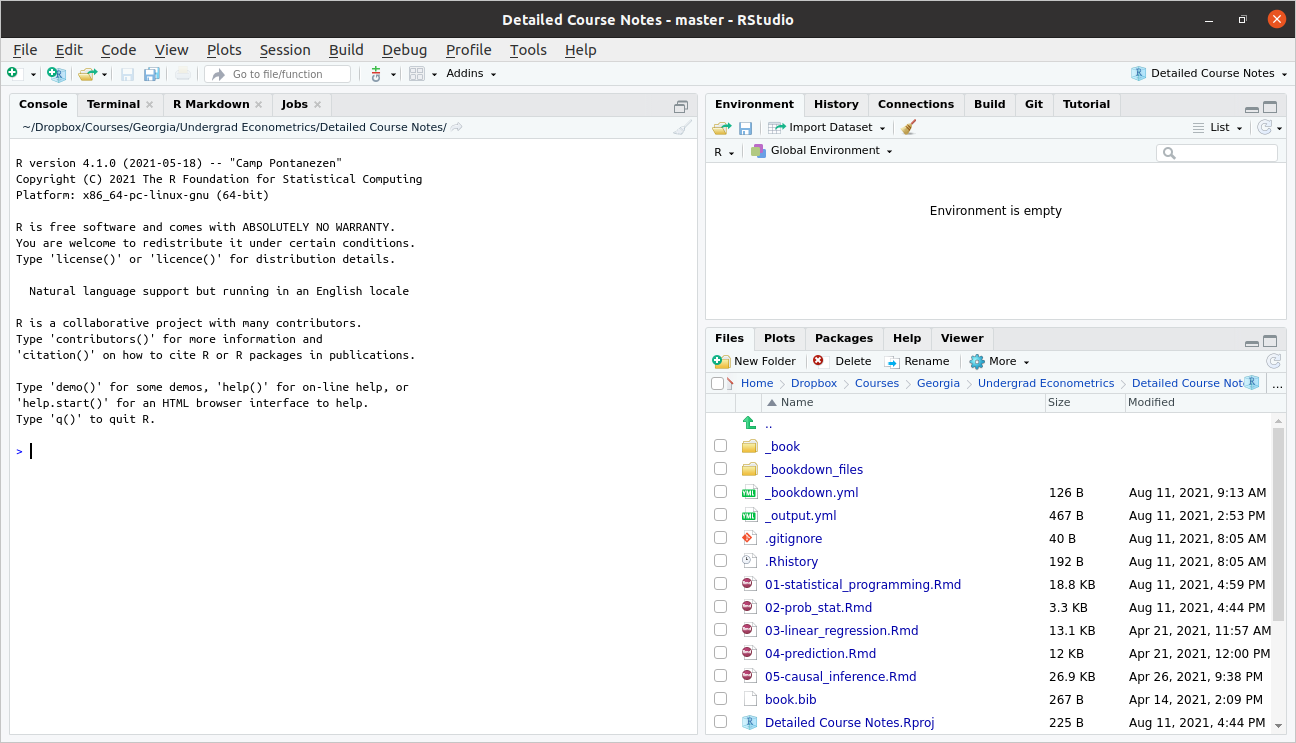
\includegraphics{open_rstudio.png}

Typically, we will write \textbf{scripts}, basically just as a way to
save the code that we have written. Go to
\texttt{File\ -\textgreater{}\ New\ File\ -\textgreater{}\ R\ Script}.
This will open up a new pane, and your screen should look something like
this

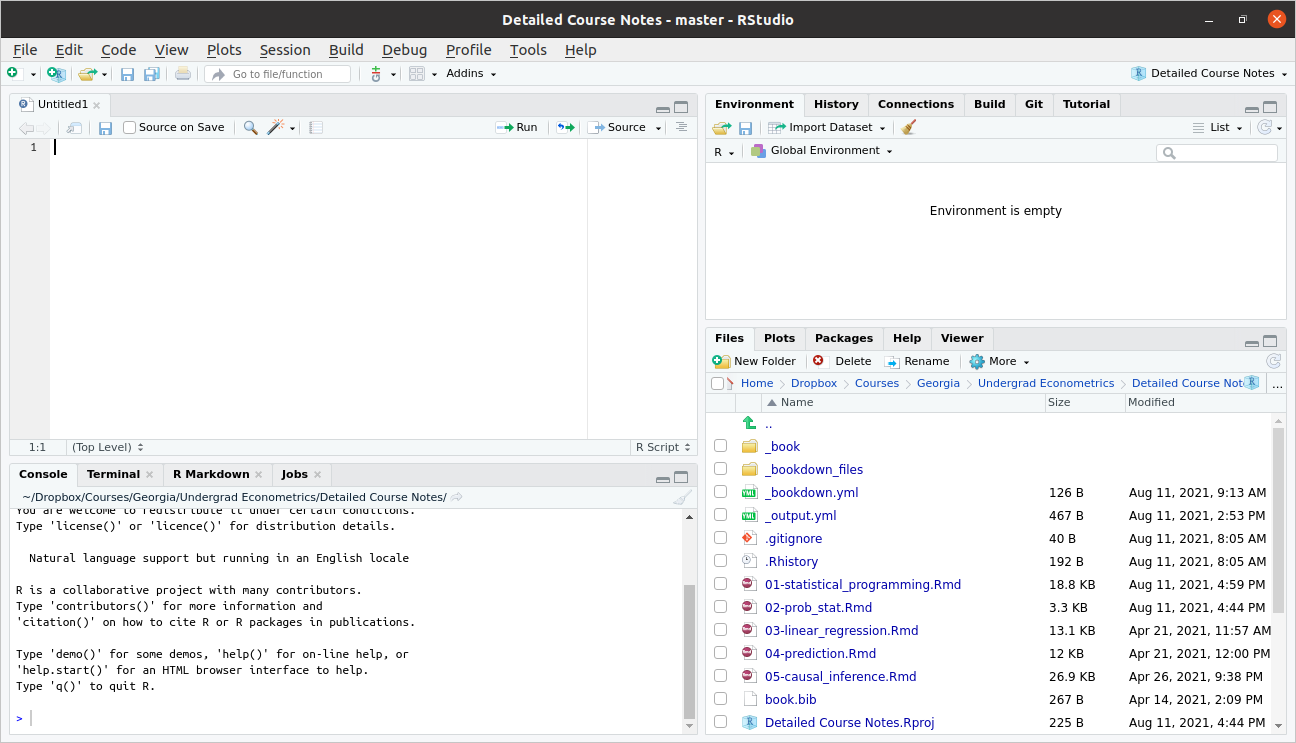
\includegraphics{rstudio_script.png}

Let's look around here. The top left pane is called the ``Source Pane''.
It is where you can write an R script. Try typing

\begin{Shaded}
\begin{Highlighting}[]
\DecValTok{1}\SpecialCharTok{+}\DecValTok{1}
\end{Highlighting}
\end{Shaded}

in that pane. This is a very simple R program. Now, type \texttt{Ctrl+s}
to save the script. This will likely prompt you to provide a name for
the script. You can call it \texttt{first\_script.R} or something like
that. The only thing that really matters is that the file name ends in
``.R'' (although you should at least give the file a reasonably
descriptive name).

Now let's move to the bottom left pane. This is called the ``Console
Pane''. It is where the actual computations happen in R (Notice that,
although we have already saved our first script, we haven't actually run
any code). Beside the blue arrow in that pane, try typing

\begin{Shaded}
\begin{Highlighting}[]
\DecValTok{2}\SpecialCharTok{+}\DecValTok{2}
\end{Highlighting}
\end{Shaded}

and then press \texttt{ENTER}. This time you should actually see the
answer.

Now, let's go back to the Source pane. Often, it is convenient to run R
programs line by line (mainly in order for it to be easy for you to
digest the results). You can do this by pressing \texttt{Ctrl+ENTER} on
any line in your script for it to run next. Try this on the first line
of your script file where we previously typed \texttt{1+1}. This code
should now run, and you should be able to see the result down in the
bottom left Console pane.

We will ignore the two panes on the right for now and come back to them
once we get a little more experience programming in R.

\section{Installing R Packages}\label{installing-r-packages}

Related Reading: IDS 1.5

When you download \texttt{R}, you get ``base'' \texttt{R}. Base R
contains ``basic'' functions that are commonly used by most R users. To
give some examples, base R gives you the ability add, subtract, divide,
or multiply numbers. Base R gives you the ability to calculate the mean
(the function is called \texttt{mean}) or standard deviation (the
function is called \texttt{sd}) of a vector of numbers.

Base R is quite powerful and probably the majority of code you will
write in R will only involve Base R.

That being said, there are many cases where it is useful to expand the
base functionality of \texttt{R}. This is done through
\textbf{packages}. Packages expand the functionality of R. R is open
source so these packages are contributed by users.

It also typically wouldn't make sense for someone to install \emph{all}
available R packages. For example, a geographer might want to install a
much different set of packages relative to an economist. Therefore, we
will typically install only the additional functionality that we
specifically want.

{Example: }In this example, we'll install the \texttt{dslabs} package
(which is from the IDS book) and the \texttt{lubridate} package (which
is a package for working with dates in R).

\begin{Shaded}
\begin{Highlighting}[]
\CommentTok{\# install dslabs package}
\FunctionTok{install.packages}\NormalTok{(}\StringTok{"dslabs"}\NormalTok{)}

\CommentTok{\# install lubridate package}
\FunctionTok{install.packages}\NormalTok{(}\StringTok{"lubridate"}\NormalTok{)}
\end{Highlighting}
\end{Shaded}

Installing a package is only the first step to using a package. You can
think of installing a package like \emph{downloading} a package. To
actually use a package, you need to load it into memory (i.e.,
``attach'' it) or at least be clear about the package where a function
that you are trying to call comes from.

{Example: } Dates can be tricky to work with in R (and in programming
languages generally). For example, they are not exactly numbers, but
they also have more structure than just a character string. The
\texttt{lubridate} package contains functions for converting
numbers/strings into dates.

\begin{Shaded}
\begin{Highlighting}[]
\NormalTok{bday }\OtherTok{\textless{}{-}} \StringTok{"07{-}15{-}1985"}
\FunctionTok{class}\NormalTok{(bday) }\CommentTok{\# R doesn\textquotesingle{}t know this is actually a date yet}
\end{Highlighting}
\end{Shaded}

\begin{verbatim}
[1] "character"
\end{verbatim}

\begin{Shaded}
\begin{Highlighting}[]
\CommentTok{\# load the package}
\FunctionTok{library}\NormalTok{(lubridate)}
\CommentTok{\# mdy stands for "month, day, year"}
\CommentTok{\# if date were in different format, could use ymd, etc.}
\NormalTok{date\_bday }\OtherTok{\textless{}{-}} \FunctionTok{mdy}\NormalTok{(bday)}
\NormalTok{date\_bday}
\end{Highlighting}
\end{Shaded}

\begin{verbatim}
[1] "1985-07-15"
\end{verbatim}

\begin{Shaded}
\begin{Highlighting}[]
\CommentTok{\# now R knows this is a date}
\FunctionTok{class}\NormalTok{(date\_bday)}
\end{Highlighting}
\end{Shaded}

\begin{verbatim}
[1] "Date"
\end{verbatim}

Another (and perhaps better) way to call a function from a package is to
use the \texttt{::} syntax. In this case, you do not need the call to
\texttt{library} from above. Instead, you can try

\begin{Shaded}
\begin{Highlighting}[]
\NormalTok{lubridate}\SpecialCharTok{::}\FunctionTok{mdy}\NormalTok{(bday)}
\end{Highlighting}
\end{Shaded}

\begin{verbatim}
[1] "1985-07-15"
\end{verbatim}

This does exactly the same thing as the code before. What is somewhat
better about this code is that it is easier to tell that the
\texttt{mdy} function came from the \texttt{lubridate} package.

\subsection{A list of useful R
packages}\label{a-list-of-useful-r-packages}

\begin{itemize}
\item
  \texttt{AER} --- package containing data from \emph{Applied
  Econometrics with R}
\item
  \texttt{wooldridge} --- package containing data from Wooldridge's text
  book
\item
  \texttt{ggplot2} --- package to produce sophisticated looking plots
\item
  \texttt{dplyr} --- package containing tools to manipulate data
\item
  \texttt{haven} --- package for loading different types of data files
\item
  \texttt{plm} --- package for working with panel data
\item
  \texttt{fixest} --- another package for working with panel data
\item
  \texttt{ivreg} --- package for IV regressions, diagnostics, etc.
\item
  \texttt{estimatr} --- package that runs regressions but with standard
  errors that economists often like more than the default options in
  \texttt{R}
\item
  \texttt{modelsummary} --- package for producing nice output of more
  than one regression and summary statistics
\end{itemize}

As of this writing, there are currently 18,004 R packages available on
CRAN (R's main repository for contributed packages).

\section{R Basics}\label{r-basics}

Related Reading: IDS 2.1

In this section, we'll start to work towards writing useful R code.

\subsection{Objects}\label{objects}

Related Reading: IDS 2.2

The very first step to writing code that can actually do something is to
able to store things. In R, we store things in \textbf{objects} (perhaps
sometimes I will also use the word variables).

Earlier, we used R to calculate \(1+1\). Let's go back to the Source
pane (top left pane in RStudio) and type

\begin{Shaded}
\begin{Highlighting}[]
\NormalTok{answer }\OtherTok{\textless{}{-}} \DecValTok{1} \SpecialCharTok{+} \DecValTok{1}
\end{Highlighting}
\end{Shaded}

Press \texttt{Ctrl+ENTER} on this line to run it. You should see the
same line down in the Console now.

Let's think carefully about what is happening here

\begin{itemize}
\item
  \texttt{answer} is the name of the variable (or object) that we are
  creating here.
\item
  the \texttt{\textless{}-} is the \textbf{assignment} operator. It
  means that we should \emph{assign} whatever is on the right hand side
  of it to the variable that is on the left hand side of it
\item
  \texttt{1+1} just computes \(1+1\) as we did earlier. Soon we will put
  more complicated expressions here.
\end{itemize}

You can think about the above code as computing \(1+1\) and then
\emph{saving} it in the variable \texttt{answer}.

{Side Comment:} The assignment operator, \texttt{\textless{}-}, is a
``less than sign'' followed by a ``hyphen''. It's often convenient
though to use the keyboard shortcut \texttt{Alt+-} (i.e., hold down
\texttt{Alt} and press the hypen key) to insert it. You can also use an
\texttt{=} for assignment, but this is less commonly done in R.

{Practice:} Try creating variable called \texttt{five\_squared} that is
equal to \(5 \times 5\) (multiplication in R is done using the
\texttt{*} symbol).

There are a number of reasons why you might like to create an object in
R. Perhaps the main one is so that you can reuse it. Let's try
multiplying \texttt{answer} by \(3\).

\begin{Shaded}
\begin{Highlighting}[]
\NormalTok{answer}\SpecialCharTok{*}\DecValTok{3}
\end{Highlighting}
\end{Shaded}

\begin{verbatim}
[1] 6
\end{verbatim}

If you wanted, you could also save this as its own variable too.

\subsection{Workspace}\label{workspace}

Related Reading: IDS 2.2

Before we move on, I just want to show you what my workspace looks like
now.

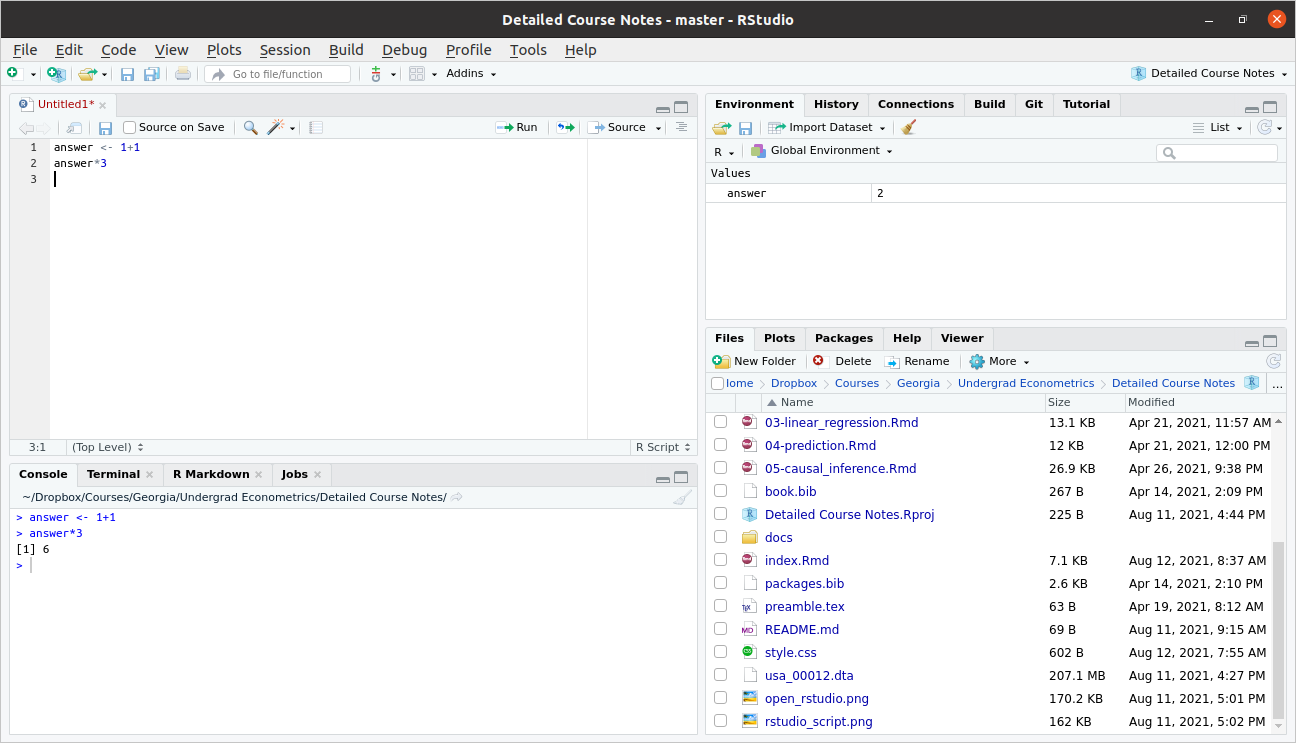
\includegraphics{rstudio_environment.png}

As we talked about above, you can see the code in my script in the
Source pane in the top left. You can also see the code that I actually
ran in the Console pane on the bottom left.

Now, take a look at the top right pane. You will see under the
Environment tab that \texttt{answer} shows up there with a value of
\texttt{2}. The Environment tab keeps track of all the variables that
you have created in your current session. A couple of other things that
might be useful to point out there.

\begin{itemize}
\item
  Later on in the class, we will often import data to work with. You
  will notice the ``Import Dataset'' button that is located in this top
  right pane. I will suggest to you a different way of importing data in
  the next section, but this is also a way to do it.
\item
  Occasionally, you might get into the case where you have saved a bunch
  of variables and it would be helpful to ``start over''. The broom in
  this pane will ``clean'' your workspace (this just means delete
  everything).
\end{itemize}

\subsection{Importing Data}\label{importing-data}

To work with actual data in R, we will need to import it. I mentioned
the ``Import Data'' button above, but let me mention a few other
possibilities here, including how to import data by writing code.

On the course website, I posted three files \texttt{firm.data.csv},
\texttt{firm\_data.RData}, and \texttt{firm\_data.dta}. All three of
these contain exactly the same small, fictitious dataset, but are saved
in different formats.

Probably the easiest way to import data in R is through the Files pane
on the bottom right. But, in order to do this, you may need to change
your \textbf{working directory}. We will do this using RStudio's user
interface in the following steps:

\begin{itemize}
\tightlist
\item
  First navigate to Sessions -\textgreater{} Set Working Directory
  -\textgreater{} Choose Directory. This will open a window that will
  allow you to choose the directory where you saved the data.
\end{itemize}

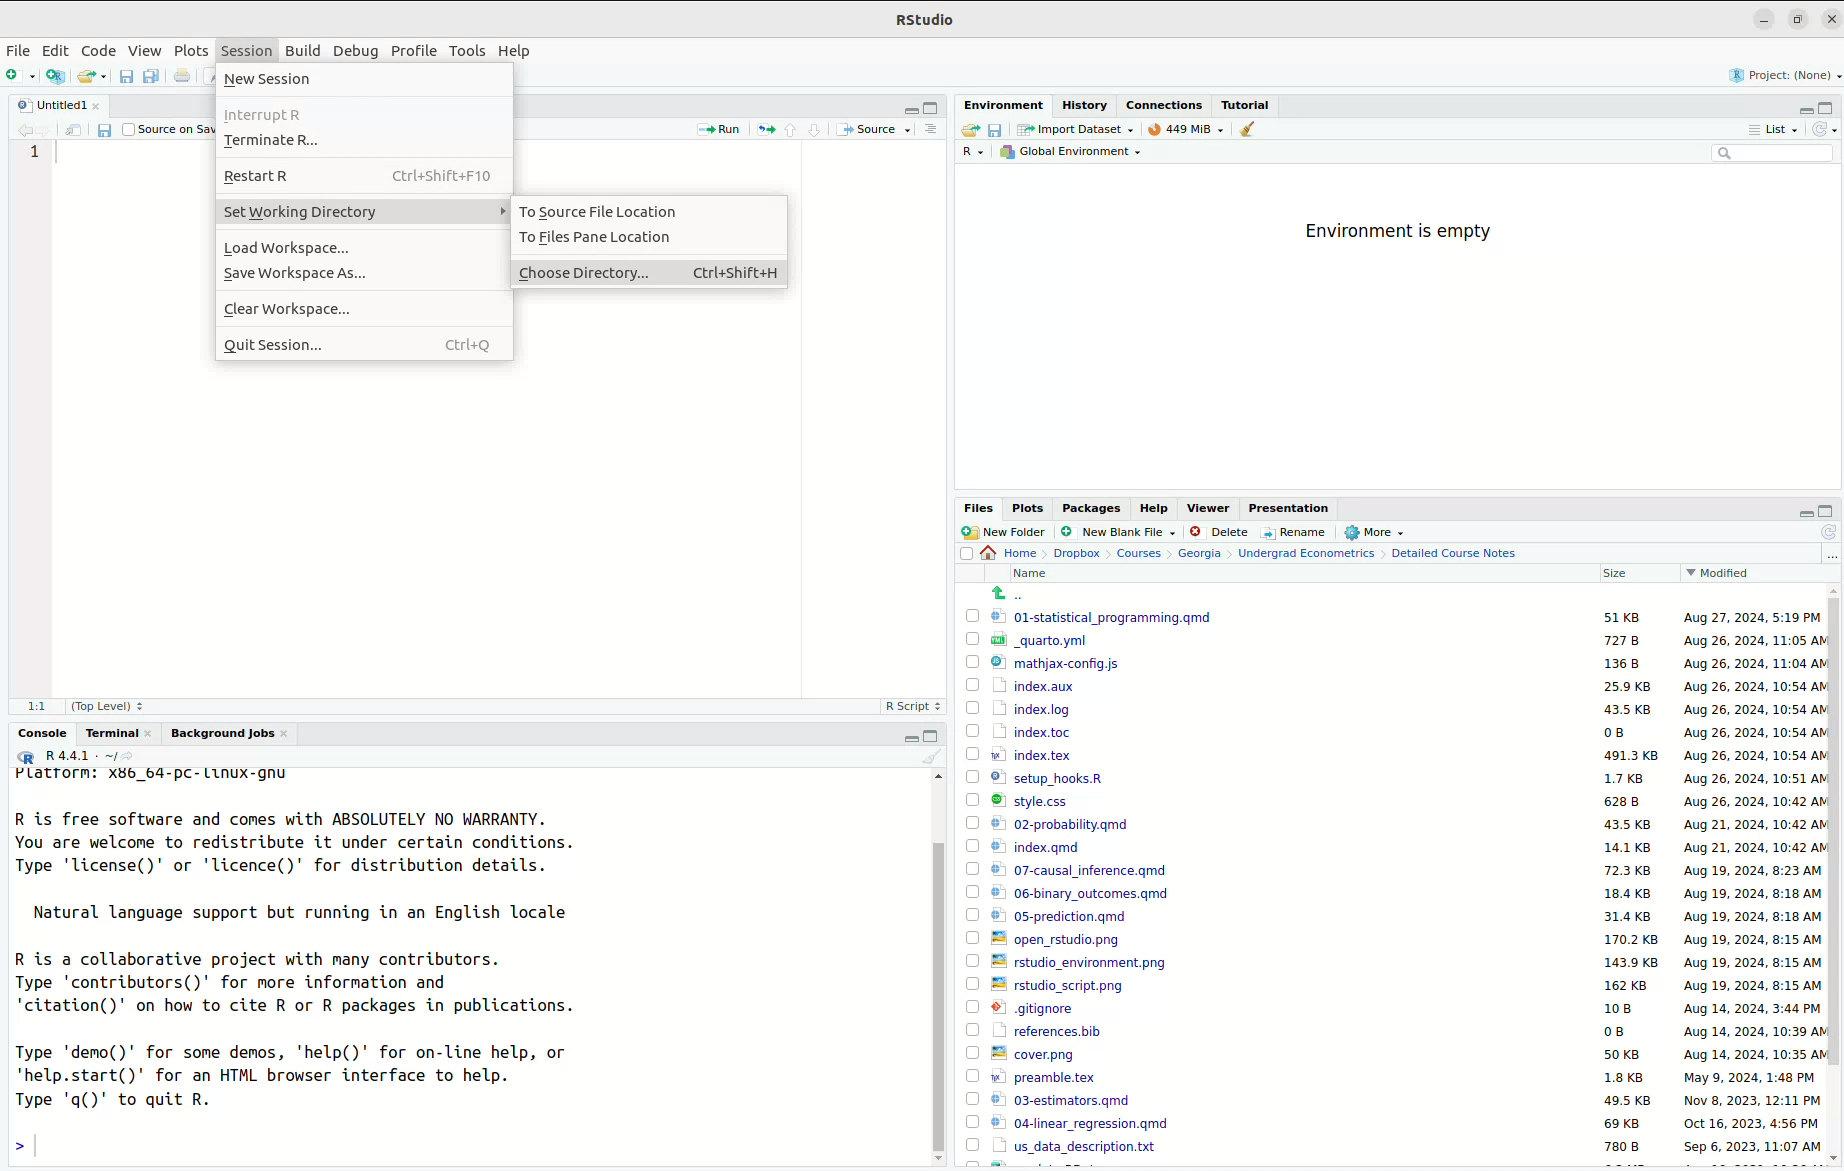
\includegraphics{set_wd.png}

\begin{itemize}
\tightlist
\item
  Next, use the menu to navigate to the place where you saved
  \texttt{firm\_data.csv}. I created a folder
  \texttt{\textasciitilde{}/Dropbox/Courses/Georgia/Undergrad\ Econometrics/24\ Fall/firm\ data/}
  and saved it there.
\end{itemize}

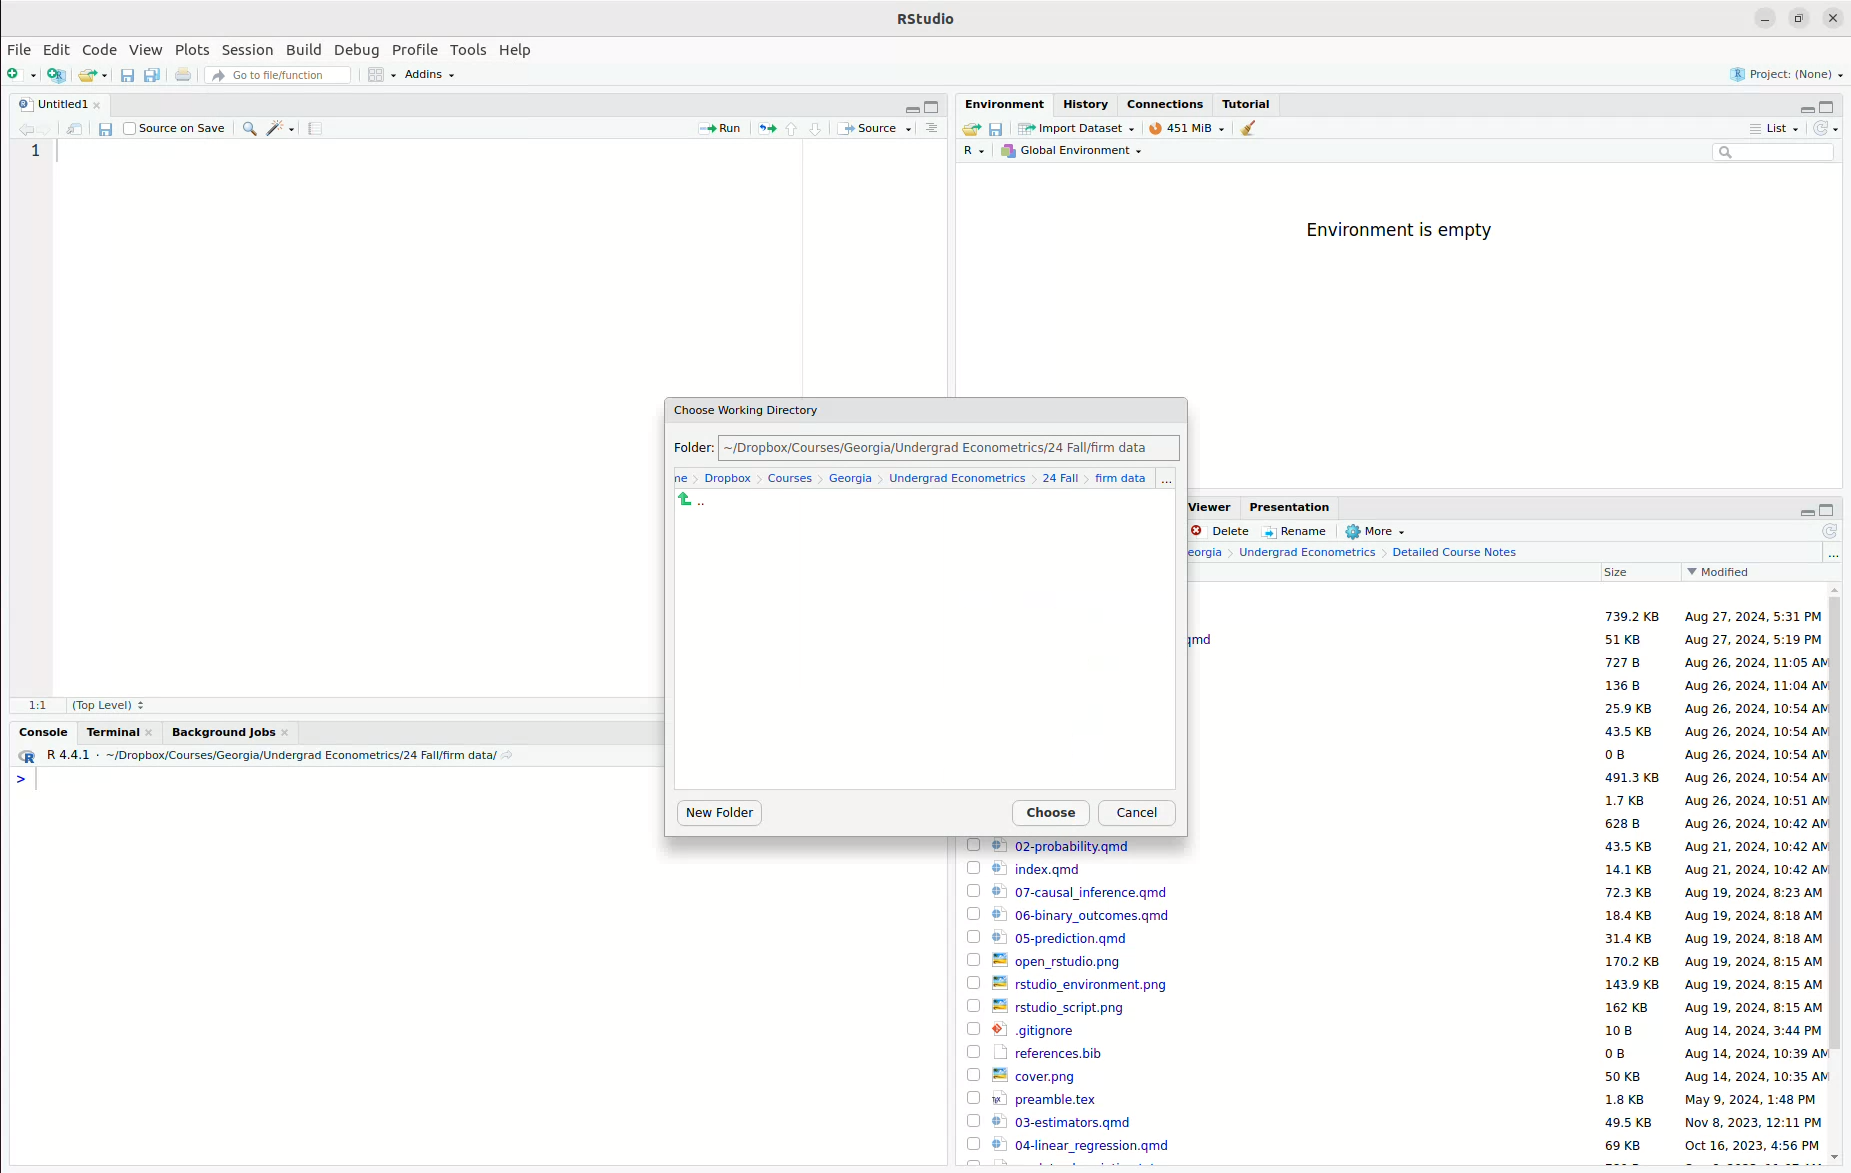
\includegraphics{set_wd2.png}

\begin{itemize}
\tightlist
\item
  Now, we have set the working directory, and this is what RStudio looks
  like for me. Notice that the working directory is now set to the
  folder where I saved the data. You can see the difference in the Files
  pane.
\end{itemize}

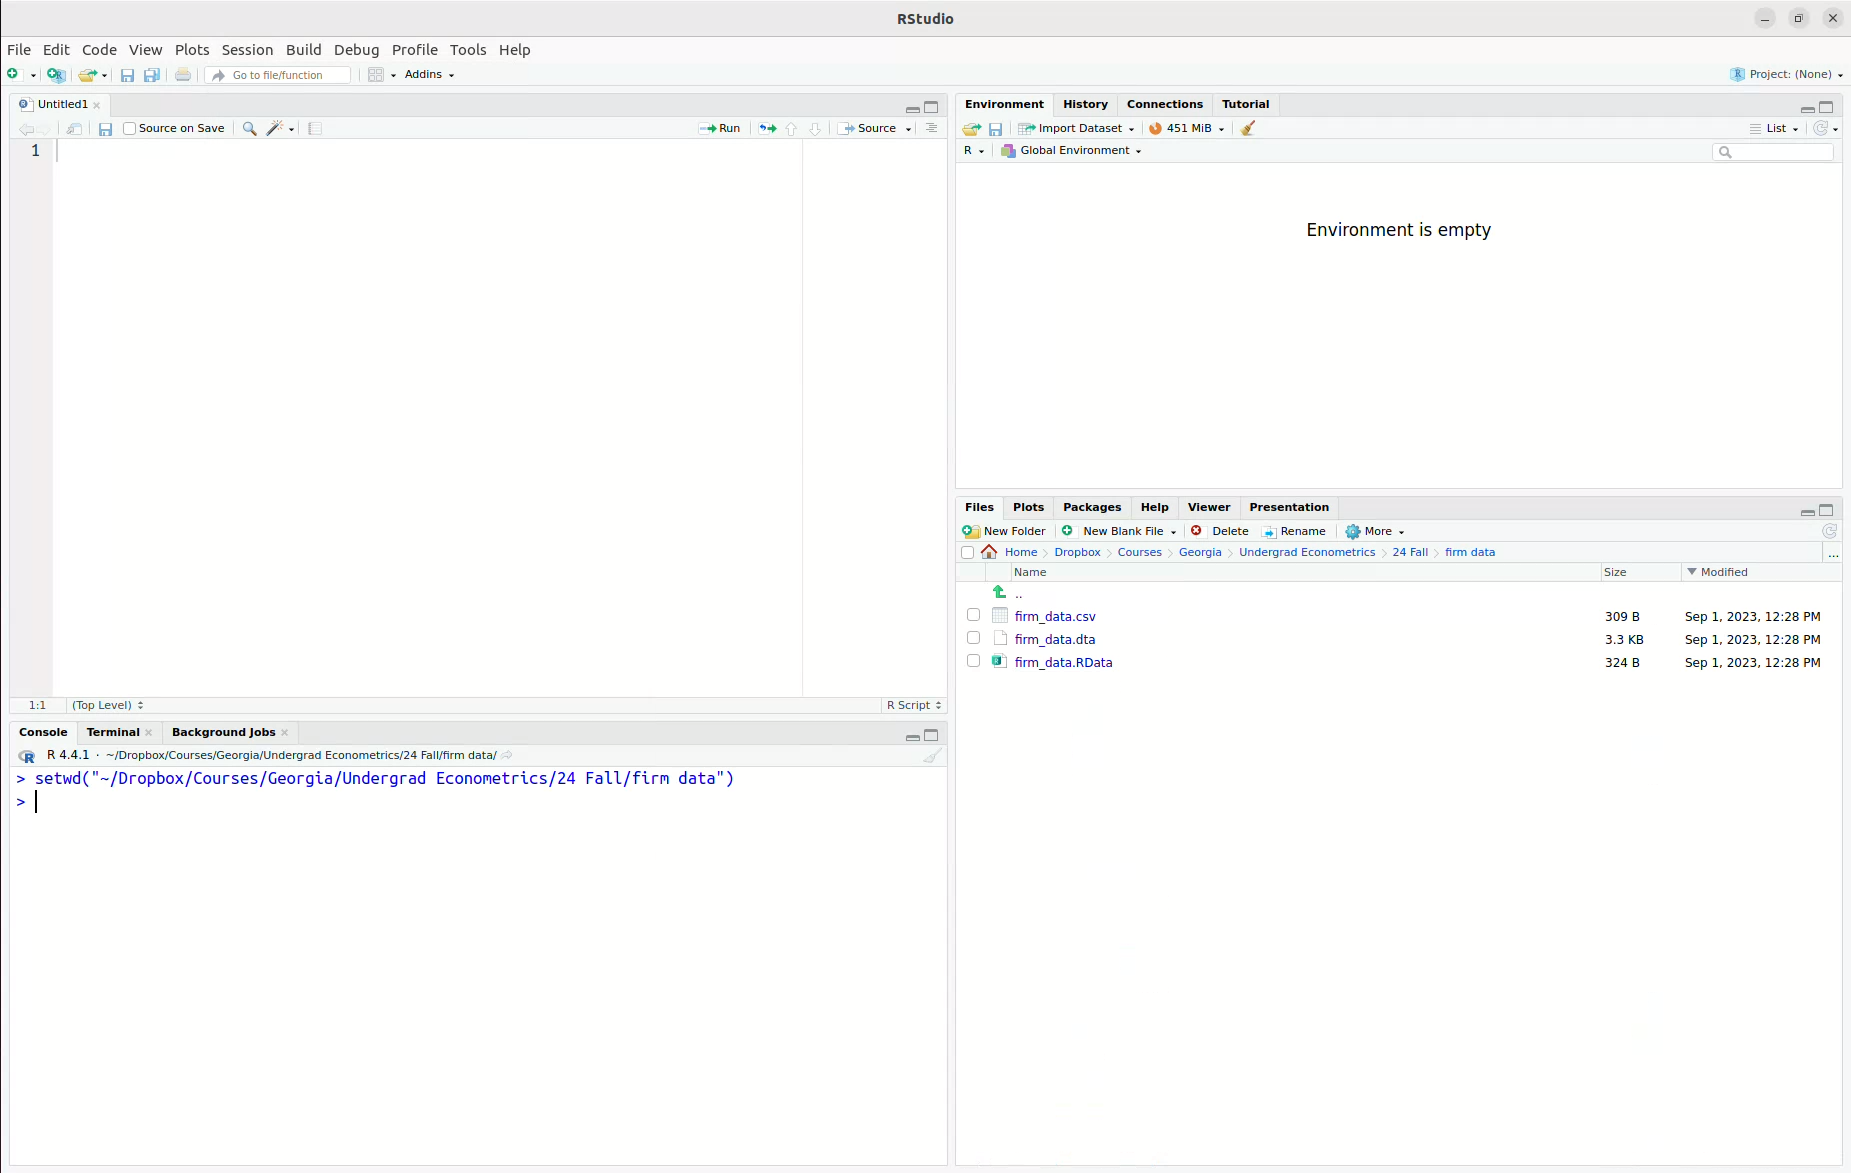
\includegraphics{set_wd3.png}

\begin{itemize}
\tightlist
\item
  Next, we will load the data, just by clicking it in the Files pane. I
  picked \texttt{firm\_data.csv}, but any of the three files will work.
  \texttt{R} is quite good at recognizing different types of data files
  and importing them, so this same procedure will work for
  \texttt{firm\_data.RData} and \texttt{firm\_data.dta} even though they
  are different types of files. Once you click it, you will get a screen
  that should look like this
\end{itemize}

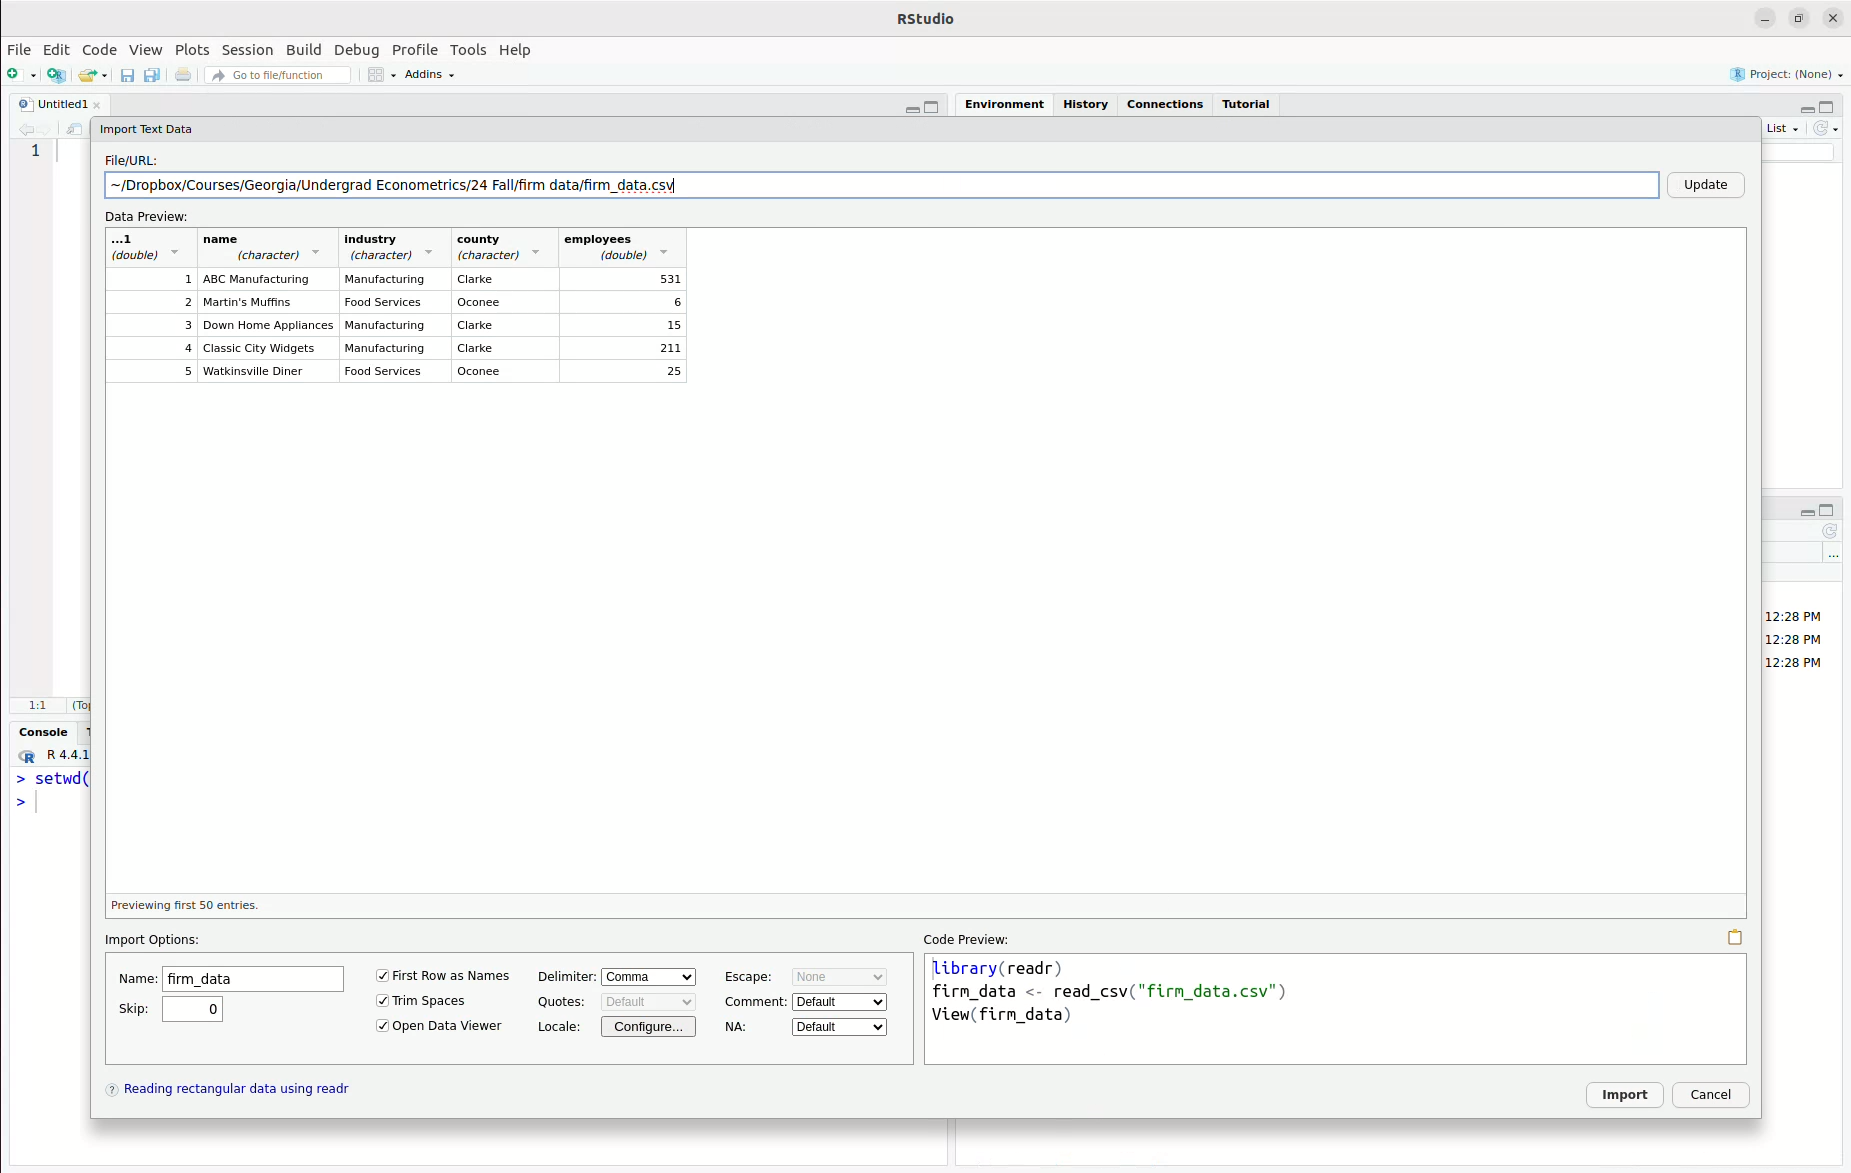
\includegraphics{import_data.png}

\begin{itemize}
\tightlist
\item
  Click ``Import'' and the data should be imported. You can see that it
  is now in the Environment pane.
\end{itemize}

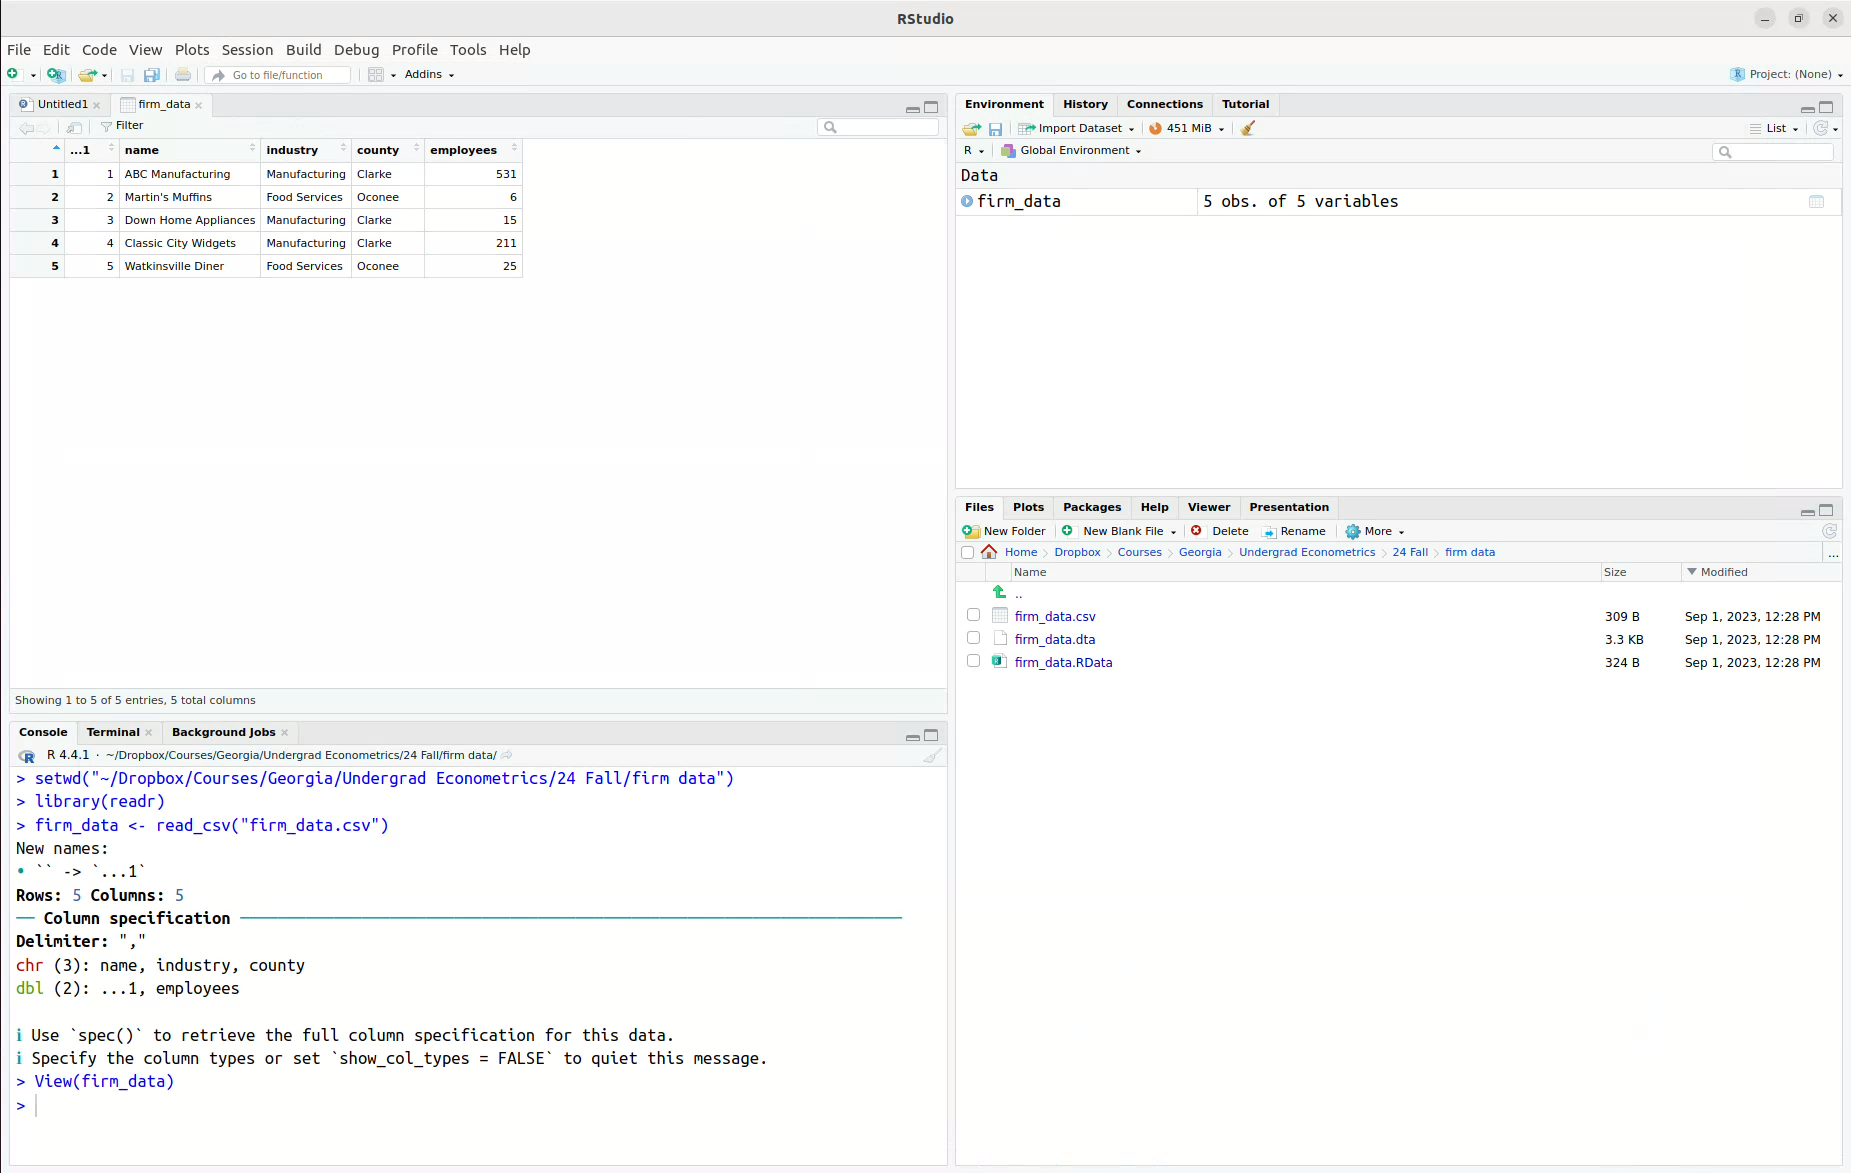
\includegraphics{import_data2.png}

Next, let's discuss how to import data by writing computer code (by the
way, this is actually what is happening behind the scenes when you
import data through the user interface as described above). ``csv''
stands for ``Comma Separated Values''. This is basically a plain text
file (e.g., try opening it in Notepad or Text Editor) where the columns
are separated by commas and the rows are separated by being on different
lines. Most any computer program can read this type of file; that is,
you could easily import this file into, say, R, Excel, or Stata. You can
import a \texttt{.csv} file using \texttt{R} code by

\begin{Shaded}
\begin{Highlighting}[]
\NormalTok{firm\_data }\OtherTok{\textless{}{-}} \FunctionTok{read.csv}\NormalTok{(}\StringTok{"firm\_data.csv"}\NormalTok{)}
\end{Highlighting}
\end{Shaded}

An \texttt{RData} file is the native format for saving data in
\texttt{R}. You can import an \texttt{RData} file using the following
command:

\begin{Shaded}
\begin{Highlighting}[]
\NormalTok{firm\_data }\OtherTok{\textless{}{-}} \FunctionTok{load}\NormalTok{(}\StringTok{"firm\_data.RData"}\NormalTok{)}
\end{Highlighting}
\end{Shaded}

Similarly, a \texttt{dta} file the native format for saving data in
Stata. You can import a \texttt{dta} file using the following command:

\begin{Shaded}
\begin{Highlighting}[]
\FunctionTok{library}\NormalTok{(haven) }\CommentTok{\# external package for reading dta file}
\NormalTok{firm\_data }\OtherTok{\textless{}{-}} \FunctionTok{read\_dta}\NormalTok{(}\StringTok{"firm\_data.dta"}\NormalTok{)}
\end{Highlighting}
\end{Shaded}

In all three cases above, what we have done is to create a new
\texttt{data.frame} (a \texttt{data.frame} is a type of object that
we'll talk about in detail later on in this chapter) called
\texttt{firm\_data} that contains the data that we were trying to load.

\bookmarksetup{startatroot}

\chapter{Programming in R}\label{programming-in-r}

\[
\newcommand{\E}{\mathbb{E}}
\renewcommand{\P}{\textrm{P}}
\let\L\relax
\newcommand{\L}{\textrm{L}} %doesn't work in .qmd, place this command at start of qmd file to use it
\newcommand{\F}{\textrm{F}}
\newcommand{\var}{\textrm{var}}
\newcommand{\cov}{\textrm{cov}}
\newcommand{\corr}{\textrm{corr}}
\newcommand{\Var}{\mathrm{Var}}
\newcommand{\Cov}{\mathrm{Cov}}
\newcommand{\Corr}{\mathrm{Corr}}
\newcommand{\sd}{\mathrm{sd}}
\newcommand{\se}{\mathrm{s.e.}}
\newcommand{\T}{T}
\newcommand{\indicator}[1]{\mathbb{1}\{#1\}}
\newcommand\independent{\perp \!\!\! \perp}
\newcommand{\N}{\mathcal{N}}
\]

\section{Functions in R}\label{functions-in-r}

Related Reading: IDS 2.2

R has a large number of helpful, built-in functions. Let's start with a
pretty representative example: computing logarithms. This can be done
using the R function \texttt{log}.

\begin{Shaded}
\begin{Highlighting}[]
\FunctionTok{log}\NormalTok{(}\DecValTok{5}\NormalTok{)}
\end{Highlighting}
\end{Shaded}

\begin{verbatim}
[1] 1.609438
\end{verbatim}

You can tell this is a function because of the parentheses. The
\texttt{5} inside of the parentheses is called the \textbf{argument} of
the function. As practice, try computing the \(\log\) of 7.

{Side Comment:} As a reminder, the logarithm of some number, let's call
it \(b\), is is the value of \(a\) that solves \(\textrm{base}^a = b\).

The default base in R is \(e \approx 2.718\), so that \texttt{log(5)}
actually computes what you might be more used to calling the ``natural
logarithm''. You can change the default value of the base by adding an
extra argument to the function.

\begin{Shaded}
\begin{Highlighting}[]
\FunctionTok{log}\NormalTok{(}\DecValTok{5}\NormalTok{, }\AttributeTok{base=}\DecValTok{10}\NormalTok{)}
\end{Highlighting}
\end{Shaded}

\begin{verbatim}
[1] 0.69897
\end{verbatim}

In order to learn about what arguments are available (and what they
mean), you can access the help files for a particular function by
running either

\begin{Shaded}
\begin{Highlighting}[]
\FunctionTok{help}\NormalTok{(log)}
\NormalTok{?log}
\end{Highlighting}
\end{Shaded}

and, of course, substituting the name of whatever function you want to
learn about in place of \texttt{log}.

In RStudio, it can also be helpful to press \texttt{Tab} and RStudio
will provide possible completions to the function you are typing as well
as what arguments can be provided to that function.

{Practice:} R has a function for computing absolute value (you'll have
to find the name of it on your own). Try computing the absolute value of
\(5\) and \(-5\). Try creating a variable called
\texttt{negative\_three} that is equal to \(-3\); then, try to compute
the absolute value of \texttt{negative\_three}.

\section{Data types}\label{data-types}

Related Reading: IDS 2.4

\subsection{Numeric Vectors}\label{numeric-vectors}

The most basic data type in \texttt{R} is the vector. In fact, above
when we created variables that were just a single number, they are
actually stored as a numeric vector.

To more explicitly create a vector, you can use the \texttt{c} function
in \texttt{R}. For example, let's create a vector called \texttt{five}
that contains the numbers 1 through 5.

\begin{Shaded}
\begin{Highlighting}[]
\NormalTok{  five }\OtherTok{\textless{}{-}} \FunctionTok{c}\NormalTok{(}\DecValTok{1}\NormalTok{,}\DecValTok{2}\NormalTok{,}\DecValTok{3}\NormalTok{,}\DecValTok{4}\NormalTok{,}\DecValTok{5}\NormalTok{)}
\end{Highlighting}
\end{Shaded}

We can print the contents of the vector \texttt{five} just by typing its
name

\begin{Shaded}
\begin{Highlighting}[]
\NormalTok{five}
\end{Highlighting}
\end{Shaded}

\begin{verbatim}
[1] 1 2 3 4 5
\end{verbatim}

Another common operation on vectors is to get a particular element of a
vector. Let me give an example

\begin{Shaded}
\begin{Highlighting}[]
\NormalTok{five[}\DecValTok{3}\NormalTok{]}
\end{Highlighting}
\end{Shaded}

\begin{verbatim}
[1] 3
\end{verbatim}

This code takes the vector \texttt{five} and returns the third element
in the vector. Notice that the above line contains braces, \texttt{{[}}
and \texttt{{]}} rather than parentheses.

If you want several different elements from a vector, you can do the
following

\begin{Shaded}
\begin{Highlighting}[]
\NormalTok{five[}\FunctionTok{c}\NormalTok{(}\DecValTok{1}\NormalTok{,}\DecValTok{4}\NormalTok{)]}
\end{Highlighting}
\end{Shaded}

\begin{verbatim}
[1] 1 4
\end{verbatim}

This code takes the vector \texttt{five} and returns the first and
fourth element in the vector.

One more useful function for vectors is the function \texttt{length}.
This tells you the number of elements in vector. For example,

\begin{Shaded}
\begin{Highlighting}[]
\FunctionTok{length}\NormalTok{(five)}
\end{Highlighting}
\end{Shaded}

\begin{verbatim}
[1] 5
\end{verbatim}

which means that there are five total elements in the vector
\texttt{five}.

\subsection{Vector arithmetic}\label{vector-arithmetic}

Related Reading: IDS 2.8

The main operations on numeric vectors are \texttt{+}, \texttt{-},
\texttt{*}, \texttt{/} which correspond to addition, subtraction,
multiplication, and division. Often, we would like to carry out these
operations on vectors.

There are two main cases. The first case is when you try to add a single
number (i.e., a scalar) to all the elements in a vector. In this setup,
the operation will happen element-wise which means the same number will
be added to all numbers in the vector. This will be clear with some
examples.

\begin{Shaded}
\begin{Highlighting}[]
\NormalTok{five }\OtherTok{\textless{}{-}} \FunctionTok{c}\NormalTok{(}\DecValTok{1}\NormalTok{,}\DecValTok{2}\NormalTok{,}\DecValTok{3}\NormalTok{,}\DecValTok{4}\NormalTok{,}\DecValTok{5}\NormalTok{)}

\CommentTok{\# adds one to each element in vector}
\NormalTok{five }\SpecialCharTok{+} \DecValTok{1}
\end{Highlighting}
\end{Shaded}

\begin{verbatim}
[1] 2 3 4 5 6
\end{verbatim}

\begin{Shaded}
\begin{Highlighting}[]
\CommentTok{\# also adds one to each element in vector}
\DecValTok{1} \SpecialCharTok{+}\NormalTok{ five}
\end{Highlighting}
\end{Shaded}

\begin{verbatim}
[1] 2 3 4 5 6
\end{verbatim}

Similar things will happen with the other mathematical operations above.
Here are some more examples:

\begin{Shaded}
\begin{Highlighting}[]
\NormalTok{five }\SpecialCharTok{*} \DecValTok{3}
\end{Highlighting}
\end{Shaded}

\begin{verbatim}
[1]  3  6  9 12 15
\end{verbatim}

\begin{Shaded}
\begin{Highlighting}[]
\NormalTok{five }\SpecialCharTok{{-}} \DecValTok{3}
\end{Highlighting}
\end{Shaded}

\begin{verbatim}
[1] -2 -1  0  1  2
\end{verbatim}

\begin{Shaded}
\begin{Highlighting}[]
\NormalTok{five }\SpecialCharTok{/} \DecValTok{3}
\end{Highlighting}
\end{Shaded}

\begin{verbatim}
[1] 0.3333333 0.6666667 1.0000000 1.3333333 1.6666667
\end{verbatim}

The other interesting case is what happens when you try to apply any of
the same mathematical operators to two different vectors.

\begin{Shaded}
\begin{Highlighting}[]
\CommentTok{\# just some random numbers}
\NormalTok{vec2 }\OtherTok{\textless{}{-}} \FunctionTok{c}\NormalTok{(}\DecValTok{8}\NormalTok{,}\SpecialCharTok{{-}}\DecValTok{3}\NormalTok{,}\DecValTok{4}\NormalTok{,}\DecValTok{1}\NormalTok{,}\DecValTok{7}\NormalTok{)}

\NormalTok{five }\SpecialCharTok{+}\NormalTok{ vec2}
\end{Highlighting}
\end{Shaded}

\begin{verbatim}
[1]  9 -1  7  5 12
\end{verbatim}

\begin{Shaded}
\begin{Highlighting}[]
\NormalTok{five }\SpecialCharTok{{-}}\NormalTok{ vec2}
\end{Highlighting}
\end{Shaded}

\begin{verbatim}
[1] -7  5 -1  3 -2
\end{verbatim}

\begin{Shaded}
\begin{Highlighting}[]
\NormalTok{five }\SpecialCharTok{*}\NormalTok{ vec2}
\end{Highlighting}
\end{Shaded}

\begin{verbatim}
[1]  8 -6 12  4 35
\end{verbatim}

\begin{Shaded}
\begin{Highlighting}[]
\NormalTok{five }\SpecialCharTok{/}\NormalTok{ vec2}
\end{Highlighting}
\end{Shaded}

\begin{verbatim}
[1]  0.1250000 -0.6666667  0.7500000  4.0000000  0.7142857
\end{verbatim}

You can immediately see what happens here. For example, for
\texttt{five\ +\ vec2}, the first element of \texttt{five} is added to
the first element of \texttt{vec2}, the second element of \texttt{five}
is added to the second element of \texttt{vec2} and so on. Similar
things happen for each of the other mathematical operations too.

There's one other case that might be interesting to consider too. What
happens if you try to apply these mathematical operations to two vectors
of different lengths? Let's find out

\begin{Shaded}
\begin{Highlighting}[]
\NormalTok{vec3 }\OtherTok{\textless{}{-}} \FunctionTok{c}\NormalTok{(}\DecValTok{2}\NormalTok{,}\DecValTok{6}\NormalTok{)}
\NormalTok{five }\SpecialCharTok{+}\NormalTok{ vec3}
\end{Highlighting}
\end{Shaded}

\begin{verbatim}
Warning in five + vec3: longer object length is not a multiple of shorter
object length
\end{verbatim}

\begin{verbatim}
[1]  3  8  5 10  7
\end{verbatim}

You'll notice that this computes \emph{something} but it also issues a
warning. What happens here is that the result is equal to the first
element of \texttt{five} plus the first element of \texttt{vec3}, the
second of \texttt{five} plus the second element of \texttt{vec3}, the
third element of \texttt{five} plus \emph{the first element of
\texttt{vec3}}, the fourth element of \texttt{five} plus \emph{the
second element of \texttt{vec3}}, and the fifth element of \texttt{five}
plus \emph{the first element of \texttt{vec3}}. What's happening here is
that, since \texttt{vec3} contains fewere elements that \texttt{five},
the elements of \texttt{vec3} are getting \emph{recycled}. In my
experience, this warning often indicates a coding mistake. There are
many cases where I want to add the same number to all elements in a
vector, and many other cases where I want to add two vectors that have
the same length, but I cannot think of any cases where I would want to
add two vectors the way that is being carried out here.

The same sort of things will happen with subtraction, multiplication,
and division (feel free to try it out).

\subsection{More helpful functions in
R}\label{more-helpful-functions-in-r}

This is definitely an incomplete list, but I'll point you here to some
more functions in R that are often helpful along with quick examples of
them.

\begin{itemize}
\item
  \texttt{seq} function --- creates a ``sequence'' of numbers

\begin{Shaded}
\begin{Highlighting}[]
\FunctionTok{seq}\NormalTok{(}\DecValTok{2}\NormalTok{,}\DecValTok{7}\NormalTok{)}
\end{Highlighting}
\end{Shaded}

\begin{verbatim}
[1] 2 3 4 5 6 7
\end{verbatim}
\item
  \texttt{sum} function --- computes the sum of a vector of numbers

\begin{Shaded}
\begin{Highlighting}[]
\FunctionTok{sum}\NormalTok{(}\FunctionTok{c}\NormalTok{(}\DecValTok{1}\NormalTok{,}\DecValTok{5}\NormalTok{,}\DecValTok{8}\NormalTok{))}
\end{Highlighting}
\end{Shaded}

\begin{verbatim}
[1] 14
\end{verbatim}
\item
  \texttt{sort}, \texttt{order}, and \texttt{rev} functions ---
  functions for understanding the order or changing the order of a
  vector

\begin{Shaded}
\begin{Highlighting}[]
\FunctionTok{sort}\NormalTok{(}\FunctionTok{c}\NormalTok{(}\DecValTok{3}\NormalTok{,}\DecValTok{1}\NormalTok{,}\DecValTok{5}\NormalTok{))}
\end{Highlighting}
\end{Shaded}

\begin{verbatim}
[1] 1 3 5
\end{verbatim}

\begin{Shaded}
\begin{Highlighting}[]
\FunctionTok{order}\NormalTok{(}\FunctionTok{c}\NormalTok{(}\DecValTok{3}\NormalTok{,}\DecValTok{1}\NormalTok{,}\DecValTok{5}\NormalTok{))}
\end{Highlighting}
\end{Shaded}

\begin{verbatim}
[1] 2 1 3
\end{verbatim}

\begin{Shaded}
\begin{Highlighting}[]
\FunctionTok{rev}\NormalTok{(}\FunctionTok{c}\NormalTok{(}\DecValTok{3}\NormalTok{,}\DecValTok{1}\NormalTok{,}\DecValTok{5}\NormalTok{))}
\end{Highlighting}
\end{Shaded}

\begin{verbatim}
[1] 5 1 3
\end{verbatim}
\item
  \texttt{\%\%} --- modulo function (i.e., returns the remainder from
  dividing one number by another)

\begin{Shaded}
\begin{Highlighting}[]
\DecValTok{8} \SpecialCharTok{\%\%} \DecValTok{3}
\end{Highlighting}
\end{Shaded}

\begin{verbatim}
[1] 2
\end{verbatim}

\begin{Shaded}
\begin{Highlighting}[]
\DecValTok{1} \SpecialCharTok{\%\%} \DecValTok{3}
\end{Highlighting}
\end{Shaded}

\begin{verbatim}
[1] 1
\end{verbatim}
\end{itemize}

{Practice:} The function \texttt{seq} contains an optional argument
\texttt{length.out}. Try running the following code and seeing if you
can figure out what \texttt{length.out} does.

\begin{Shaded}
\begin{Highlighting}[]
\FunctionTok{seq}\NormalTok{(}\DecValTok{1}\NormalTok{,}\DecValTok{10}\NormalTok{,}\AttributeTok{length.out=}\DecValTok{5}\NormalTok{)}
\FunctionTok{seq}\NormalTok{(}\DecValTok{1}\NormalTok{,}\DecValTok{10}\NormalTok{,}\AttributeTok{length.out=}\DecValTok{10}\NormalTok{)}
\FunctionTok{seq}\NormalTok{(}\FloatTok{1.10}\NormalTok{,}\AttributeTok{length.out=}\DecValTok{20}\NormalTok{)}
\end{Highlighting}
\end{Shaded}

\subsection{Other types of vectors}\label{other-types-of-vectors}

There are other types of vectors in R too. Probably the main two other
types of vectors are \textbf{character vectors} and \textbf{logical
vectors}. We'll talk about character vectors here and defer logical
vectors until later. Character vectors are often referred to as
\textbf{strings}.

We can create a character vector as follows

\begin{Shaded}
\begin{Highlighting}[]
\NormalTok{string1 }\OtherTok{\textless{}{-}} \StringTok{"econometrics"}
\NormalTok{string2 }\OtherTok{\textless{}{-}} \StringTok{"class"}
\NormalTok{string1}
\end{Highlighting}
\end{Shaded}

\begin{verbatim}
[1] "econometrics"
\end{verbatim}

The above code creates two character vectors and then prints the first
one.

{Side Comment} \texttt{c} stands for ``concatenate''. Concatenate is a
computer science word that means to combine two vectors. Probably the
most well known version of this is ``string concatenation'' that
combines two vectors of characters. Here is an example of string
concatenation.

\begin{Shaded}
\begin{Highlighting}[]
\FunctionTok{c}\NormalTok{(string1, string2)}
\end{Highlighting}
\end{Shaded}

\begin{verbatim}
[1] "econometrics" "class"       
\end{verbatim}

Sometimes string concatenation means to put two (or more strings) into
the same string. This can be done using the \texttt{paste} command in R.

\begin{Shaded}
\begin{Highlighting}[]
\FunctionTok{paste}\NormalTok{(string1, string2)}
\end{Highlighting}
\end{Shaded}

\begin{verbatim}
[1] "econometrics class"
\end{verbatim}

Notice that \texttt{paste} puts in a space between \texttt{string1} and
\texttt{string2}. For practice, see if you can find an argument to the
\texttt{paste} function that allows you to remove the space between the
two strings.

\subsection{Data Frames}\label{data-frames}

Another very important type of object in R is the \textbf{data frame}. I
think it is helpful to think of a data frame as being very similar to an
Excel spreadsheet --- sort of like a matrix or a two-dimensional array.
Each row typically corresponds to a particular observation, and each
column typically provides the value of a particular variable for that
observation.

Just to give a simple example, suppose that we had firm-level data about
the name of the firm, what industry a firm was in, what county they were
located in, and their number of employees. I created a data frame like
this (it is totally made up, BTW) and show it to you next

\begin{Shaded}
\begin{Highlighting}[]
\NormalTok{firm\_data}
\end{Highlighting}
\end{Shaded}

\begin{longtable}[]{@{}lllr@{}}
\toprule\noalign{}
name & industry & county & employees \\
\midrule\noalign{}
\endhead
\bottomrule\noalign{}
\endlastfoot
ABC Manufacturing & Manufacturing & Clarke & 531 \\
Martin's Muffins & Food Services & Oconee & 6 \\
Down Home Appliances & Manufacturing & Clarke & 15 \\
Classic City Widgets & Manufacturing & Clarke & 211 \\
Watkinsville Diner & Food Services & Oconee & 25 \\
\end{longtable}

{Side Comment:} If you are following along on R, I created this data
frame using the following code

\begin{Shaded}
\begin{Highlighting}[]
\NormalTok{firm\_data }\OtherTok{\textless{}{-}} \FunctionTok{data.frame}\NormalTok{(}\AttributeTok{name=}\FunctionTok{c}\NormalTok{(}\StringTok{"ABC Manufacturing"}\NormalTok{, }\StringTok{"Martin}\SpecialCharTok{\textbackslash{}\textquotesingle{}}\StringTok{s Muffins"}\NormalTok{, }\StringTok{"Down Home Appliances"}\NormalTok{, }\StringTok{"Classic City Widgets"}\NormalTok{, }\StringTok{"Watkinsville Diner"}\NormalTok{),}
                        \AttributeTok{industry=}\FunctionTok{c}\NormalTok{(}\StringTok{"Manufacturing"}\NormalTok{, }\StringTok{"Food Services"}\NormalTok{, }\StringTok{"Manufacturing"}\NormalTok{, }\StringTok{"Manufacturing"}\NormalTok{, }\StringTok{"Food Services"}\NormalTok{),}
                        \AttributeTok{county=}\FunctionTok{c}\NormalTok{(}\StringTok{"Clarke"}\NormalTok{, }\StringTok{"Oconee"}\NormalTok{, }\StringTok{"Clarke"}\NormalTok{, }\StringTok{"Clarke"}\NormalTok{, }\StringTok{"Oconee"}\NormalTok{),}
                        \AttributeTok{employees=}\FunctionTok{c}\NormalTok{(}\DecValTok{531}\NormalTok{, }\DecValTok{6}\NormalTok{, }\DecValTok{15}\NormalTok{, }\DecValTok{211}\NormalTok{, }\DecValTok{25}\NormalTok{))}
\end{Highlighting}
\end{Shaded}

This is also the same data that we loaded earlier in Section 2.3.

Often, we'll like to access a particular column in a data frame. For
example, you might want to calculate the average number of employees
across all the firms in our data.

Typically, the easiest way to do this, is to use the \textbf{accessor}
symbol, which is \texttt{\$} in R. This will make more sense with an
example:

\begin{Shaded}
\begin{Highlighting}[]
\NormalTok{firm\_data}\SpecialCharTok{$}\NormalTok{employees}
\end{Highlighting}
\end{Shaded}

\begin{verbatim}
[1] 531   6  15 211  25
\end{verbatim}

\texttt{firm\_data\$employees} just provides the column called
``employees'' in the data frame called ``firm\_data''. You can also
notice that \texttt{firm\_data\$employees} is just a numeric vector.
This means that you can apply any of the functions that we have been
covering on it

\begin{Shaded}
\begin{Highlighting}[]
\FunctionTok{mean}\NormalTok{(firm\_data}\SpecialCharTok{$}\NormalTok{employees)}
\end{Highlighting}
\end{Shaded}

\begin{verbatim}
[1] 157.6
\end{verbatim}

\begin{Shaded}
\begin{Highlighting}[]
\FunctionTok{log}\NormalTok{(firm\_data}\SpecialCharTok{$}\NormalTok{employees)}
\end{Highlighting}
\end{Shaded}

\begin{verbatim}
[1] 6.274762 1.791759 2.708050 5.351858 3.218876
\end{verbatim}

{Side Comment:} Notice that the function \texttt{mean} and \texttt{log}
behave differently. \texttt{mean} calculates the average over all the
elements in the vector \texttt{firm\_data\$employees} and therefore
returns a single number. \texttt{log} calculates the logarithm of each
element in the vector \texttt{firm\_data\$employees} and therefore
returns a numeric vector with five elements.

{Side Comment:}

The \texttt{\$} is not the only way to access the elements in a data
frame. You can also access them by their position. For example, if you
want whatever is in the third row and second column of the data frame,
you can get it by

\begin{Shaded}
\begin{Highlighting}[]
\NormalTok{firm\_data[}\DecValTok{3}\NormalTok{,}\DecValTok{2}\NormalTok{]}
\end{Highlighting}
\end{Shaded}

\begin{verbatim}
[1] "Manufacturing"
\end{verbatim}

Sometimes it is also convenient to recover a particular row or column by
its position in the data frame. Here is an example of recovering the
entire fourth row

\begin{Shaded}
\begin{Highlighting}[]
\NormalTok{firm\_data[}\DecValTok{4}\NormalTok{,]}
\end{Highlighting}
\end{Shaded}

\begin{verbatim}
                  name      industry county employees
4 Classic City Widgets Manufacturing Clarke       211
\end{verbatim}

Notice that you just leave the ``column index'' (which is the second
one) blank

{Side Comment:} One other thing that sometimes takes some getting used
to is that, for programming in general, you have to be very precise.
Suppose you were to make a very small typo. R is not going to understand
what you mean. See if you can spot the typo in the next line of code.

\begin{Shaded}
\begin{Highlighting}[]
\NormalTok{firm\_data}\SpecialCharTok{$}\NormalTok{employes}
\end{Highlighting}
\end{Shaded}

\begin{verbatim}
NULL
\end{verbatim}

A few more useful functions for working with data frames are:

\begin{itemize}
\item
  \texttt{nrow} and \texttt{ncol} --- returns the number of rows or
  columns in the data frame
\item
  \texttt{colnames} and \texttt{rownames} --- returns the names of the
  columns or rows
\end{itemize}

\subsection{Lists}\label{lists}

Vectors and data frames are the main two types of objects that we'll use
this semester, but let me give you a quick overview of a few other types
of objects. Let's start with \textbf{lists}. Lists are very generic in
the sense that they can carry around complicated data. If you are
familiar with any object oriented programming language like Java or C++,
they have the flavor of an ``object'', in the object-oriented sense.

I'm not sure if we will see any examples this semester where you
\emph{have} to use a list. But here is an example. Suppose that we
wanted to put the vector that we created earlier \texttt{five} and the
data frame that we created earlier \texttt{firm\_data} into the same
object. We could do it as follows

\begin{Shaded}
\begin{Highlighting}[]
\NormalTok{unusual\_list }\OtherTok{\textless{}{-}} \FunctionTok{list}\NormalTok{(}\AttributeTok{numbers=}\NormalTok{five, }\AttributeTok{df=}\NormalTok{firm\_data)}
\end{Highlighting}
\end{Shaded}

You can access the elements of a list in a few different ways. Sometimes
it is convenient to access them via the \texttt{\$}

\begin{Shaded}
\begin{Highlighting}[]
\NormalTok{unusual\_list}\SpecialCharTok{$}\NormalTok{numbers}
\end{Highlighting}
\end{Shaded}

\begin{verbatim}
[1] 1 2 3 4 5
\end{verbatim}

Other times, it is convenient to access them via their position in the
list

\begin{Shaded}
\begin{Highlighting}[]
\NormalTok{unusual\_list[[}\DecValTok{2}\NormalTok{]] }\CommentTok{\# notice the double brackets}
\end{Highlighting}
\end{Shaded}

\begin{verbatim}
                  name      industry county employees
1    ABC Manufacturing Manufacturing Clarke       531
2     Martin's Muffins Food Services Oconee         6
3 Down Home Appliances Manufacturing Clarke        15
4 Classic City Widgets Manufacturing Clarke       211
5   Watkinsville Diner Food Services Oconee        25
\end{verbatim}

\subsection{Matrices}\label{matrices}

Matrices are very similar to data frames, but the data should all be of
the same type. Matrices are very useful in some numerical calculations
that are beyond the scope of this class. Here is an example of a matrix.

\begin{Shaded}
\begin{Highlighting}[]
\NormalTok{mat }\OtherTok{\textless{}{-}} \FunctionTok{matrix}\NormalTok{(}\FunctionTok{c}\NormalTok{(}\DecValTok{1}\NormalTok{,}\DecValTok{2}\NormalTok{,}\DecValTok{3}\NormalTok{,}\DecValTok{4}\NormalTok{), }\AttributeTok{nrow=}\DecValTok{2}\NormalTok{, }\AttributeTok{byrow=}\ConstantTok{TRUE}\NormalTok{)}
\NormalTok{mat}
\end{Highlighting}
\end{Shaded}

\begin{verbatim}
     [,1] [,2]
[1,]    1    2
[2,]    3    4
\end{verbatim}

You can access elements of a matrix by their position in the matrix,
just like for the data frame above.

\begin{Shaded}
\begin{Highlighting}[]
\CommentTok{\# first row, second column}
\NormalTok{mat[}\DecValTok{1}\NormalTok{,}\DecValTok{2}\NormalTok{]}
\end{Highlighting}
\end{Shaded}

\begin{verbatim}
[1] 2
\end{verbatim}

\begin{Shaded}
\begin{Highlighting}[]
\CommentTok{\# all rows in second column}
\NormalTok{mat[,}\DecValTok{2}\NormalTok{] }
\end{Highlighting}
\end{Shaded}

\begin{verbatim}
[1] 2 4
\end{verbatim}

\subsection{Factors}\label{factors}

Sometimes variables in economics are \textbf{categorical}. This sort of
variable is somewhat between a numeric variable and a string. In
\texttt{R}, categorical variables are called \textbf{factors}.

A good example of a categorical variable is
\texttt{firm\_data\$industry}. It tells you the ``category'' of the
industry that a firm is in.

Oftentimes, we may have to tell R that a variable is a ``factor'' rather
than just a string. Let's create a variable called \texttt{industry}
that contains the industry from \texttt{firm\_data} but as a factor.

\begin{Shaded}
\begin{Highlighting}[]
\NormalTok{industry }\OtherTok{\textless{}{-}} \FunctionTok{as.factor}\NormalTok{(firm\_data}\SpecialCharTok{$}\NormalTok{industry)}
\NormalTok{industry}
\end{Highlighting}
\end{Shaded}

\begin{verbatim}
[1] Manufacturing Food Services Manufacturing Manufacturing Food Services
Levels: Food Services Manufacturing
\end{verbatim}

A useful package for working with factor variables is the
\texttt{forcats} package.

\subsection{Understanding an object in
R}\label{understanding-an-object-in-r}

Sometimes you may be in the case where there is a variable where you
don't know what exactly it contains. Some functions that are helpful in
this case are

\begin{itemize}
\item
  \texttt{class} --- tells you, err, the class of an object (i.e., its
  ``type'')
\item
  \texttt{head} --- shows you the ``beginning'' of an object; this is
  especially helpful for large objects (like some data frames)
\item
  \texttt{str} --- stands for ``structure'' of an object
\end{itemize}

Let's try these out

\begin{Shaded}
\begin{Highlighting}[]
\FunctionTok{class}\NormalTok{(firm\_data)}
\end{Highlighting}
\end{Shaded}

\begin{verbatim}
[1] "data.frame"
\end{verbatim}

\begin{Shaded}
\begin{Highlighting}[]
\CommentTok{\# typically would show the first five rows of a data frame,}
\CommentTok{\# but that is the whole data frame here}
\FunctionTok{head}\NormalTok{(firm\_data) }
\end{Highlighting}
\end{Shaded}

\begin{verbatim}
                  name      industry county employees
1    ABC Manufacturing Manufacturing Clarke       531
2     Martin's Muffins Food Services Oconee         6
3 Down Home Appliances Manufacturing Clarke        15
4 Classic City Widgets Manufacturing Clarke       211
5   Watkinsville Diner Food Services Oconee        25
\end{verbatim}

\begin{Shaded}
\begin{Highlighting}[]
\FunctionTok{str}\NormalTok{(firm\_data)}
\end{Highlighting}
\end{Shaded}

\begin{verbatim}
'data.frame':   5 obs. of  4 variables:
 $ name     : chr  "ABC Manufacturing" "Martin's Muffins" "Down Home Appliances" "Classic City Widgets" ...
 $ industry : chr  "Manufacturing" "Food Services" "Manufacturing" "Manufacturing" ...
 $ county   : chr  "Clarke" "Oconee" "Clarke" "Clarke" ...
 $ employees: num  531 6 15 211 25
\end{verbatim}

{Practice:} Try running \texttt{class}, \texttt{head}, and \texttt{str}
on the vector \texttt{five} that we created earlier.

\section{Logicals}\label{logicals}

Related Reading: IDS 2.9

All programming languages have ways of tracking whether variables meet
certain criteria. These are often called Booleans or Logicals. For us,
this will particularly come up in the context of subsetting data (i.e.,
selecting data based on some condition) and in running particular
portions of code based on some condition.

Some main logical operators are \texttt{==}, \texttt{\textless{}=},
\texttt{\textgreater{}=}, \texttt{\textless{}}, \texttt{\textgreater{}}
corresponding to whether or not two things are equal, less than or equal
to, greater than or equal, strictly less than, and strictly greater
than. These can be applied to vectors. And the comparisons result in
either \texttt{TRUE} or \texttt{FALSE}. Here are some examples

\begin{Shaded}
\begin{Highlighting}[]
\NormalTok{five }\OtherTok{\textless{}{-}} \FunctionTok{c}\NormalTok{(}\DecValTok{1}\NormalTok{,}\DecValTok{2}\NormalTok{,}\DecValTok{3}\NormalTok{,}\DecValTok{4}\NormalTok{,}\DecValTok{5}\NormalTok{)}

\CommentTok{\# only 3 is equal to 3}
\NormalTok{five }\SpecialCharTok{==} \DecValTok{3}
\end{Highlighting}
\end{Shaded}

\begin{verbatim}
[1] FALSE FALSE  TRUE FALSE FALSE
\end{verbatim}

\begin{Shaded}
\begin{Highlighting}[]
\CommentTok{\# 1,2,3 are all less than or equal to 3}
\NormalTok{five }\SpecialCharTok{\textless{}=} \DecValTok{3}
\end{Highlighting}
\end{Shaded}

\begin{verbatim}
[1]  TRUE  TRUE  TRUE FALSE FALSE
\end{verbatim}

\begin{Shaded}
\begin{Highlighting}[]
\CommentTok{\# 3,4,5, are all greater than or equal to 3}
\NormalTok{five }\SpecialCharTok{\textgreater{}=} \DecValTok{3}
\end{Highlighting}
\end{Shaded}

\begin{verbatim}
[1] FALSE FALSE  TRUE  TRUE  TRUE
\end{verbatim}

\begin{Shaded}
\begin{Highlighting}[]
\CommentTok{\# 1,2 are strictly less than 3}
\NormalTok{five }\SpecialCharTok{\textless{}} \DecValTok{3}
\end{Highlighting}
\end{Shaded}

\begin{verbatim}
[1]  TRUE  TRUE FALSE FALSE FALSE
\end{verbatim}

\begin{Shaded}
\begin{Highlighting}[]
\CommentTok{\# 4,5 are strictly greater than 3}
\NormalTok{five }\SpecialCharTok{\textgreater{}} \DecValTok{3}
\end{Highlighting}
\end{Shaded}

\begin{verbatim}
[1] FALSE FALSE FALSE  TRUE  TRUE
\end{verbatim}

{Example: }Often, we might be interested in learning about a subset of
our data. As a simple example, using our \texttt{firm\_data} from
earlier, you could imagine being interested in average employment for
manufacturing firms.

We can do this using the \texttt{subset} function along with the logical
operations we've learned in this section.

\begin{Shaded}
\begin{Highlighting}[]
\NormalTok{manufacturing\_firms }\OtherTok{\textless{}{-}} \FunctionTok{subset}\NormalTok{(firm\_data, industry}\SpecialCharTok{==}\StringTok{"Manufacturing"}\NormalTok{)}
\FunctionTok{mean}\NormalTok{(manufacturing\_firms}\SpecialCharTok{$}\NormalTok{employees)}
\end{Highlighting}
\end{Shaded}

\begin{verbatim}
[1] 252.3333
\end{verbatim}

As practice, try creating a subset of \texttt{firm\_data} based on firms
having more than 100 employees.

\subsection{Additional Logical
Operators}\label{additional-logical-operators}

Related Reading: IDS 2.9

There are a number of additional logical operators that can be useful in
practice. Here, we quickly cover several more.

\begin{itemize}
\item
  \texttt{!=} --- not equal

\begin{Shaded}
\begin{Highlighting}[]
\FunctionTok{c}\NormalTok{(}\DecValTok{1}\NormalTok{,}\DecValTok{2}\NormalTok{,}\DecValTok{3}\NormalTok{) }\SpecialCharTok{!=} \DecValTok{3}
\end{Highlighting}
\end{Shaded}

\begin{verbatim}
[1]  TRUE  TRUE FALSE
\end{verbatim}
\item
  We can link together multiple logical comparisons. If we want to check
  whether multiple conditions hold, we can use ``logical AND''
  \texttt{\&}; if we want to check whether any of multiple conditions
  hold, we can use ``logical OR'' \texttt{\textbar{}}.

\begin{Shaded}
\begin{Highlighting}[]
\CommentTok{\# AND}
\NormalTok{( }\FunctionTok{c}\NormalTok{(}\DecValTok{1}\NormalTok{,}\DecValTok{2}\NormalTok{,}\DecValTok{3}\NormalTok{,}\DecValTok{4}\NormalTok{,}\DecValTok{5}\NormalTok{) }\SpecialCharTok{\textgreater{}=} \DecValTok{3}\NormalTok{ ) }\SpecialCharTok{\&}\NormalTok{ ( }\FunctionTok{c}\NormalTok{(}\DecValTok{1}\NormalTok{,}\DecValTok{2}\NormalTok{,}\DecValTok{3}\NormalTok{,}\DecValTok{4}\NormalTok{,}\DecValTok{5}\NormalTok{) }\SpecialCharTok{\textless{}} \DecValTok{5}\NormalTok{ )}
\end{Highlighting}
\end{Shaded}

\begin{verbatim}
[1] FALSE FALSE  TRUE  TRUE FALSE
\end{verbatim}

\begin{Shaded}
\begin{Highlighting}[]
\CommentTok{\# OR}
\NormalTok{( }\FunctionTok{c}\NormalTok{(}\DecValTok{1}\NormalTok{,}\DecValTok{2}\NormalTok{,}\DecValTok{3}\NormalTok{,}\DecValTok{4}\NormalTok{,}\DecValTok{5}\NormalTok{) }\SpecialCharTok{\textgreater{}=} \DecValTok{4}\NormalTok{ ) }\SpecialCharTok{|}\NormalTok{ ( }\FunctionTok{c}\NormalTok{(}\DecValTok{1}\NormalTok{,}\DecValTok{2}\NormalTok{,}\DecValTok{3}\NormalTok{,}\DecValTok{4}\NormalTok{,}\DecValTok{5}\NormalTok{) }\SpecialCharTok{\textless{}} \DecValTok{2}\NormalTok{ )}
\end{Highlighting}
\end{Shaded}

\begin{verbatim}
[1]  TRUE FALSE FALSE  TRUE  TRUE
\end{verbatim}
\item
  \texttt{\%in\%} --- checks whether the elements of one vector show up
  \emph{in} another vector

\begin{Shaded}
\begin{Highlighting}[]
\CommentTok{\# 1 is in the 2nd vector, but 7 is not}
\FunctionTok{c}\NormalTok{(}\DecValTok{1}\NormalTok{,}\DecValTok{7}\NormalTok{) }\SpecialCharTok{\%in\%} \FunctionTok{c}\NormalTok{(}\DecValTok{1}\NormalTok{,}\DecValTok{2}\NormalTok{,}\DecValTok{3}\NormalTok{,}\DecValTok{4}\NormalTok{,}\DecValTok{5}\NormalTok{)}
\end{Highlighting}
\end{Shaded}

\begin{verbatim}
[1]  TRUE FALSE
\end{verbatim}
\item
  Often it is useful to check whether any logical conditions are true or
  all logical conditions are true. This can be done as follows

\begin{Shaded}
\begin{Highlighting}[]
\CommentTok{\# this one is TRUE because 1 is in the 2nd vector  }
\FunctionTok{any}\NormalTok{(}\FunctionTok{c}\NormalTok{(}\DecValTok{1}\NormalTok{,}\DecValTok{7}\NormalTok{) }\SpecialCharTok{\%in\%} \FunctionTok{c}\NormalTok{(}\DecValTok{1}\NormalTok{,}\DecValTok{2}\NormalTok{,}\DecValTok{3}\NormalTok{,}\DecValTok{4}\NormalTok{,}\DecValTok{5}\NormalTok{))}
\end{Highlighting}
\end{Shaded}

\begin{verbatim}
[1] TRUE
\end{verbatim}

\begin{Shaded}
\begin{Highlighting}[]
\CommentTok{\# this one is FALSE because 7 is not in the 2nd vector}
\FunctionTok{all}\NormalTok{(}\FunctionTok{c}\NormalTok{(}\DecValTok{1}\NormalTok{,}\DecValTok{7}\NormalTok{) }\SpecialCharTok{\%in\%} \FunctionTok{c}\NormalTok{(}\DecValTok{1}\NormalTok{,}\DecValTok{2}\NormalTok{,}\DecValTok{3}\NormalTok{,}\DecValTok{4}\NormalTok{,}\DecValTok{5}\NormalTok{))}
\end{Highlighting}
\end{Shaded}

\begin{verbatim}
[1] FALSE
\end{verbatim}
\end{itemize}

\section{Programming basics}\label{programming-basics}

\subsection{Writing functions}\label{writing-functions}

Related Reading: IDS 3.2

It is often helpful to write your own functions in R. If you ever find
yourself repeating the same code over and over, this suggests that you
should write this code as a function and repeatedly call the function.

Suppose we are interesting in solving the quadratic equation \[
  ax^2 + bx + c = 0
\] If you remember the quadratic formula, the solution to this equation
is \[
  x = \frac{-b \pm \sqrt{b^2-4ac}}{2a}
\] It would be tedious to calculate this by hand (especially if we
wanted to calculate it for many different values of \(a\), \(b\), and
\(c\)), so let's write a function to do it.

\begin{Shaded}
\begin{Highlighting}[]
\NormalTok{quadratic\_solver }\OtherTok{\textless{}{-}} \ControlFlowTok{function}\NormalTok{(a, b, c) \{}
\NormalTok{  root1 }\OtherTok{\textless{}{-}}\NormalTok{ ( }\SpecialCharTok{{-}}\NormalTok{b }\SpecialCharTok{+} \FunctionTok{sqrt}\NormalTok{(b}\SpecialCharTok{\^{}}\DecValTok{2} \SpecialCharTok{{-}} \DecValTok{4}\SpecialCharTok{*}\NormalTok{a}\SpecialCharTok{*}\NormalTok{c) ) }\SpecialCharTok{/} \DecValTok{2}\SpecialCharTok{*}\NormalTok{a}
\NormalTok{  root1}
\NormalTok{\}}
\end{Highlighting}
\end{Shaded}

Before we try this out, let's notice a few things. First, while this
particular function is for solving the quadratic equation, this is quite
representative of what a function looks like in R.

\begin{itemize}
\item
  \texttt{quadratic\_solver} --- This is the name of the function. It's
  good to give your function a descriptive name related to what it does.
  But you could call it anything you want. If you wanted to call this
  function \texttt{uga}, it would still work.
\item
  the part \texttt{\textless{}-\ function} finishes off assigning the
  function the name \texttt{quadratic\_solver} and implies that we are
  writing down a function rather than a \texttt{vector} or
  \texttt{data.frame} or something else. This part will show up in all
  function definitions.
\item
  the part \texttt{(a,\ b,\ c)}, \texttt{a}, \texttt{b}, and \texttt{c}
  are the names of the \emph{arguments} to the function. In a minute
  when we call the function, we need to tell the function the particular
  values of \texttt{a}, \texttt{b}, and \texttt{c} for which to solve
  the quadratic equation. We could name these whatever we want, but,
  again, it is good to have descriptive names. When you write a
  different function, it can have as many arguments as you want it to
  have.
\item
  the part \texttt{\{\ ...\ \}} everything that the function does should
  go between the curly brackets
\item
  the line
  \texttt{root1\ \textless{}-\ (\ -b\ +\ sqrt(b\^{}2\ -\ 4*a*c)\ )\ /\ 2*a}
  contains the main thing that is calculated by our function. Notice
  that we only calculate one of the ``roots'' (i.e., solutions to the
  quadratic equation) because of the \(+\) in this expression.
\item
  the line \texttt{root1} R returns whatever variable is on the last
  line of the function. It might be somewhat more clear to write
  \texttt{return(root1)}. The behavior of the code would be exactly the
  same, but it is just the more common ``style'' in R programming to not
  include the explicit \texttt{return}.
\end{itemize}

Now let's try out our function

\begin{Shaded}
\begin{Highlighting}[]
\CommentTok{\# solves quadratic equation for a=1, b=4, c=3}
\FunctionTok{quadratic\_solver}\NormalTok{(}\DecValTok{1}\NormalTok{,}\DecValTok{4}\NormalTok{,}\DecValTok{3}\NormalTok{)}
\end{Highlighting}
\end{Shaded}

\begin{verbatim}
[1] -1
\end{verbatim}

\begin{Shaded}
\begin{Highlighting}[]
\CommentTok{\# solves quadratic equation for a={-}1, b=5, c=10}
\FunctionTok{quadratic\_solver}\NormalTok{(}\SpecialCharTok{{-}}\DecValTok{1}\NormalTok{,}\DecValTok{5}\NormalTok{,}\DecValTok{10}\NormalTok{)}
\end{Highlighting}
\end{Shaded}

\begin{verbatim}
[1] -1.531129
\end{verbatim}

Two last things that are worth pointing out about functions:

\begin{itemize}
\item
  Functions in R can be set up to take default values for some of their
  arguments
\item
  Because the arguments have names, if you are explicit about the name
  of the argument, then the order of the argument does not matter.
\end{itemize}

To give examples, let's write a slightly modified version of our
function to solve quadratic equations.

\begin{Shaded}
\begin{Highlighting}[]
\NormalTok{quadratic\_solver2 }\OtherTok{\textless{}{-}} \ControlFlowTok{function}\NormalTok{(}\AttributeTok{a=}\DecValTok{1}\NormalTok{, b, c) \{}
\NormalTok{  root1 }\OtherTok{\textless{}{-}}\NormalTok{ ( }\SpecialCharTok{{-}}\NormalTok{b }\SpecialCharTok{+} \FunctionTok{sqrt}\NormalTok{(b}\SpecialCharTok{\^{}}\DecValTok{2} \SpecialCharTok{{-}} \DecValTok{4}\SpecialCharTok{*}\NormalTok{a}\SpecialCharTok{*}\NormalTok{c) ) }\SpecialCharTok{/} \DecValTok{2}\SpecialCharTok{*}\NormalTok{a}
\NormalTok{  root1}
\NormalTok{\}}
\end{Highlighting}
\end{Shaded}

The only thing different here is that \texttt{a} takes the default value
of 1. Now let's try some different calls to \texttt{quadratic\_solver}
and \texttt{quadratic\_solver2}

\begin{Shaded}
\begin{Highlighting}[]
\CommentTok{\# solve again for a=1,b=4,c=3}
\FunctionTok{quadratic\_solver2}\NormalTok{(}\AttributeTok{b=}\DecValTok{4}\NormalTok{,}\AttributeTok{c=}\DecValTok{3}\NormalTok{)}
\end{Highlighting}
\end{Shaded}

\begin{verbatim}
[1] -1
\end{verbatim}

\begin{Shaded}
\begin{Highlighting}[]
\CommentTok{\# replace default and change order}
\FunctionTok{quadratic\_solver2}\NormalTok{(}\AttributeTok{c=}\DecValTok{10}\NormalTok{,}\AttributeTok{b=}\DecValTok{5}\NormalTok{,}\AttributeTok{a=}\SpecialCharTok{{-}}\DecValTok{1}\NormalTok{)}
\end{Highlighting}
\end{Shaded}

\begin{verbatim}
[1] -1.531129
\end{verbatim}

\begin{Shaded}
\begin{Highlighting}[]
\CommentTok{\# no default set for quadratic\_solver so it will crash if a not provided}
\FunctionTok{quadratic\_solver}\NormalTok{(}\AttributeTok{b=}\DecValTok{4}\NormalTok{,}\AttributeTok{c=}\DecValTok{3}\NormalTok{)}
\end{Highlighting}
\end{Shaded}

\begin{verbatim}
Error in quadratic_solver(b = 4, c = 3): argument "a" is missing, with no default
\end{verbatim}

\subsection{if/else}\label{ifelse}

Related Reading: IDS 3.1

Often when writing code, you will want to do different things depending
on some condition. Let's write a function that takes in the number of
employees that are in a firm and prints ``large'' if the firm has more
than 100 employees and ``small'' otherwise.

\begin{Shaded}
\begin{Highlighting}[]
\NormalTok{large\_or\_small }\OtherTok{\textless{}{-}} \ControlFlowTok{function}\NormalTok{(employees) \{}
  \ControlFlowTok{if}\NormalTok{ (employees }\SpecialCharTok{\textgreater{}} \DecValTok{100}\NormalTok{) \{}
    \FunctionTok{print}\NormalTok{(}\StringTok{"large"}\NormalTok{)}
\NormalTok{  \} }\ControlFlowTok{else}\NormalTok{ \{}
    \FunctionTok{print}\NormalTok{(}\StringTok{"small"}\NormalTok{)}
\NormalTok{  \}}
\NormalTok{\}}
\end{Highlighting}
\end{Shaded}

I think, at this point, this code should make sense to you. The only new
thing is the if/else. The following is not code that will actually run
but is just to help understand the logic of if/else.

\begin{Shaded}
\begin{Highlighting}[]
\ControlFlowTok{if}\NormalTok{ (condition) \{}
  \CommentTok{\# do something}
\NormalTok{\} }\ControlFlowTok{else}\NormalTok{ \{}
  \CommentTok{\# do something else}
\NormalTok{\}}
\end{Highlighting}
\end{Shaded}

All that happens with if/else is that we check whether
\texttt{condition} evaluate to \texttt{TRUE} or \texttt{FALSE}. If it is
\texttt{TRUE}, the code will do whatever is inside the first set of
brackets; if it is \texttt{FALSE}, the code will do whatever is in the
set of brackets following \texttt{else}.

\subsection{for loops}\label{for-loops}

Related Reading: IDS 3.4

Often, we need to run the same code over and over again. A \texttt{for}
loop is a main programming tool for this case (\texttt{for} loops show
up in pretty much all programming languages).

We'll have more realistic examples later on in the semester, but we'll
do something trivial for now.

\begin{Shaded}
\begin{Highlighting}[]
\NormalTok{out }\OtherTok{\textless{}{-}} \FunctionTok{c}\NormalTok{()}
\ControlFlowTok{for}\NormalTok{ (i }\ControlFlowTok{in} \DecValTok{1}\SpecialCharTok{:}\DecValTok{10}\NormalTok{) \{}
\NormalTok{  out[i] }\OtherTok{\textless{}{-}}\NormalTok{ i}\SpecialCharTok{*}\DecValTok{3}
\NormalTok{\}}
\NormalTok{out}
\end{Highlighting}
\end{Shaded}

\begin{verbatim}
 [1]  3  6  9 12 15 18 21 24 27 30
\end{verbatim}

The above code, starts with \(i=1\), calculates \(i*3\) (which is 3),
and then stores that result in the first element of the vector
\texttt{out}, then \(i\) increases to 2, the code calculates \(i*3\)
(which is now 6), and stores this result in the second element of
\texttt{out}, and so on through \(i=10\).

\subsection{Vectorization}\label{vectorization}

Related Reading: IDS 3.5

Vectorizing functions is a relatively advanced topic in R programming,
but it is an important one, so I am including it here.

Because we will often be working with data, we will often be performing
the same operation on all of the observations in the data. For example,
suppose that you wanted to take the logarithm of the number of employees
for all the firms in \texttt{firm\_data}. One way to do this is to use a
\texttt{for} loop, but this code would be a bit of a mess. Instead, the
function \texttt{log} is \textbf{vectorized} --- this means that if we
apply it to a vector, it will calculate the logarithm of each element in
the vector. Besides this, vectorized functions are often faster than
\texttt{for} loops.

Not all functions are vectorized though. Let's go back to our function
earlier called \texttt{large\_or\_small}. This took in the number of
employees at a firm and then printed ``large'' if the firm had more than
100 employees and ``small'' otherwise. Let's see what happens if we call
this function on a vector of employees (Ideally, we'd like the function
to be applied to each element in the vector).

\begin{Shaded}
\begin{Highlighting}[]
\NormalTok{employees }\OtherTok{\textless{}{-}}\NormalTok{ firm\_data}\SpecialCharTok{$}\NormalTok{employees}
\NormalTok{employees}
\end{Highlighting}
\end{Shaded}

\begin{verbatim}
[1] 531   6  15 211  25
\end{verbatim}

\begin{Shaded}
\begin{Highlighting}[]
\FunctionTok{large\_or\_small}\NormalTok{(employees)}
\end{Highlighting}
\end{Shaded}

\begin{verbatim}
Error in if (employees > 100) {: the condition has length > 1
\end{verbatim}

This is not what we wanted to have happen. Instead of determining
whether each firm was large or small, we get an error basically said
that something may be going wrong here. What's going on here is that the
function \texttt{large\_or\_small} is not vectorized.

In order to vectorize a function, we can use one of a number of
``apply'' functions in R. I'll list them here

\begin{itemize}
\item
  \texttt{sapply} --- this stands for ``simplify'' apply; it ``applies''
  the function to all the elements in the vector or list that you pass
  in and then tries to ``simplify'' the result
\item
  \texttt{lapply} --- stands for ``list'' apply; applies a function to
  all elements in a vector or list and then returns a list
\item
  \texttt{vapply} --- stands for ``vector'' apply; applies a function to
  all elements in a vector or list and then returns a vector
\item
  \texttt{apply} --- applies a function to either the rows or columns of
  a matrix-like object (i.e., a matrix or a data frame) depending on the
  value of the argument \texttt{MARGIN}
\end{itemize}

Let's use \texttt{sapply} to vectorize \texttt{large\_or\_small}.

\begin{Shaded}
\begin{Highlighting}[]
\NormalTok{large\_or\_small\_vectorized }\OtherTok{\textless{}{-}} \ControlFlowTok{function}\NormalTok{(employees\_vec) \{}
  \FunctionTok{sapply}\NormalTok{(employees\_vec, }\AttributeTok{FUN =}\NormalTok{ large\_or\_small)}
\NormalTok{\}}
\end{Highlighting}
\end{Shaded}

All that this will do is call the function \texttt{large\_or\_small} for
each element in the vector \texttt{employees}. Let's see it in action

\begin{Shaded}
\begin{Highlighting}[]
\FunctionTok{large\_or\_small\_vectorized}\NormalTok{(employees)}
\end{Highlighting}
\end{Shaded}

\begin{verbatim}
[1] "large"
[1] "small"
[1] "small"
[1] "large"
[1] "small"
\end{verbatim}

\begin{verbatim}
[1] "large" "small" "small" "large" "small"
\end{verbatim}

This is what we were hoping for.

{Side Comment:} I also typically replace most all \texttt{for} loops
with an \texttt{apply} function. In most cases, I don't think there is
much of a performance gain, but the code seems easier to read (or at
least more concise).

Earlier we wrote a function to take a vector of numbers from 1 to 10 and
multiply all of them by 3. Here's how you could do this using
\texttt{sapply}

\begin{Shaded}
\begin{Highlighting}[]
\FunctionTok{sapply}\NormalTok{(}\DecValTok{1}\SpecialCharTok{:}\DecValTok{10}\NormalTok{, }\ControlFlowTok{function}\NormalTok{(i) i}\SpecialCharTok{*}\DecValTok{3}\NormalTok{)}
\end{Highlighting}
\end{Shaded}

\begin{verbatim}
 [1]  3  6  9 12 15 18 21 24 27 30
\end{verbatim}

which is considerably shorter.

One last thing worth pointing out though is that multiplication is
already vectorized, so you don't actually need to do \texttt{sapply} or
the \texttt{for} loop; a better way is just

\begin{Shaded}
\begin{Highlighting}[]
\NormalTok{(}\DecValTok{1}\SpecialCharTok{:}\DecValTok{10}\NormalTok{)}\SpecialCharTok{*}\DecValTok{3}
\end{Highlighting}
\end{Shaded}

\begin{verbatim}
 [1]  3  6  9 12 15 18 21 24 27 30
\end{verbatim}

{Side Comment:} A relatively popular alternative to \texttt{apply}
functions are \texttt{map} functions provided in the \texttt{purrr}
package.

{Side Comment:} It's often helpful to have a vectorized version of
if/else. In \texttt{R}, this is available in the function
\texttt{ifelse}. Here is an alternative way to vectorize the function
\texttt{large\_or\_small}:

\begin{Shaded}
\begin{Highlighting}[]
\NormalTok{large\_or\_small\_vectorized2 }\OtherTok{\textless{}{-}} \ControlFlowTok{function}\NormalTok{(employees\_vec) \{}
  \FunctionTok{ifelse}\NormalTok{(employees\_vec }\SpecialCharTok{\textgreater{}} \DecValTok{100}\NormalTok{, }\StringTok{"large"}\NormalTok{, }\StringTok{"small"}\NormalTok{)}
\NormalTok{\}}
\FunctionTok{large\_or\_small\_vectorized2}\NormalTok{(firm\_data}\SpecialCharTok{$}\NormalTok{employees)}
\end{Highlighting}
\end{Shaded}

\begin{verbatim}
[1] "large" "small" "small" "large" "small"
\end{verbatim}

Here you can see that \texttt{ifelse} makes every comparison in its
first argument, and then returns the second element for every
\texttt{TRUE} coming from the first argument, and returns the third
element for every \texttt{FALSE} coming from the first argument.

\texttt{ifelse} also works with vectors in the second and third element.
For example:

\begin{Shaded}
\begin{Highlighting}[]
  \FunctionTok{ifelse}\NormalTok{(}\FunctionTok{c}\NormalTok{(}\DecValTok{1}\NormalTok{,}\DecValTok{3}\NormalTok{,}\DecValTok{5}\NormalTok{) }\SpecialCharTok{\textless{}} \DecValTok{4}\NormalTok{, }\AttributeTok{yes=}\FunctionTok{c}\NormalTok{(}\DecValTok{1}\NormalTok{,}\DecValTok{2}\NormalTok{,}\DecValTok{3}\NormalTok{), }\AttributeTok{no=}\FunctionTok{c}\NormalTok{(}\DecValTok{4}\NormalTok{,}\DecValTok{5}\NormalTok{,}\DecValTok{6}\NormalTok{))}
\end{Highlighting}
\end{Shaded}

\begin{verbatim}
[1] 1 2 6
\end{verbatim}

which picks up 1 and 2 from the second (\texttt{yes}) argument and 6
from the third (\texttt{no}) argument.

\section{Reproducible Research}\label{reproducible-research}

Related Reading: IDS Ch. 20

R has very useful tools for mix code and writing to produce reports (or,
for our purpose, homeworks and project).

As of this writing, the most common way to do this seems to be switching
from Rmarkdown to Quarto. I am going to explain how to create a Quarto
document below, but, if you are familiar with Rmarkdown, the workflow is
going to be very similar.

To create a new Quaro document, click
\texttt{File\ -\textgreater{}\ New\ File\ -\textgreater{}\ Quarto\ Document}.
That will open up a menu that looks like the following

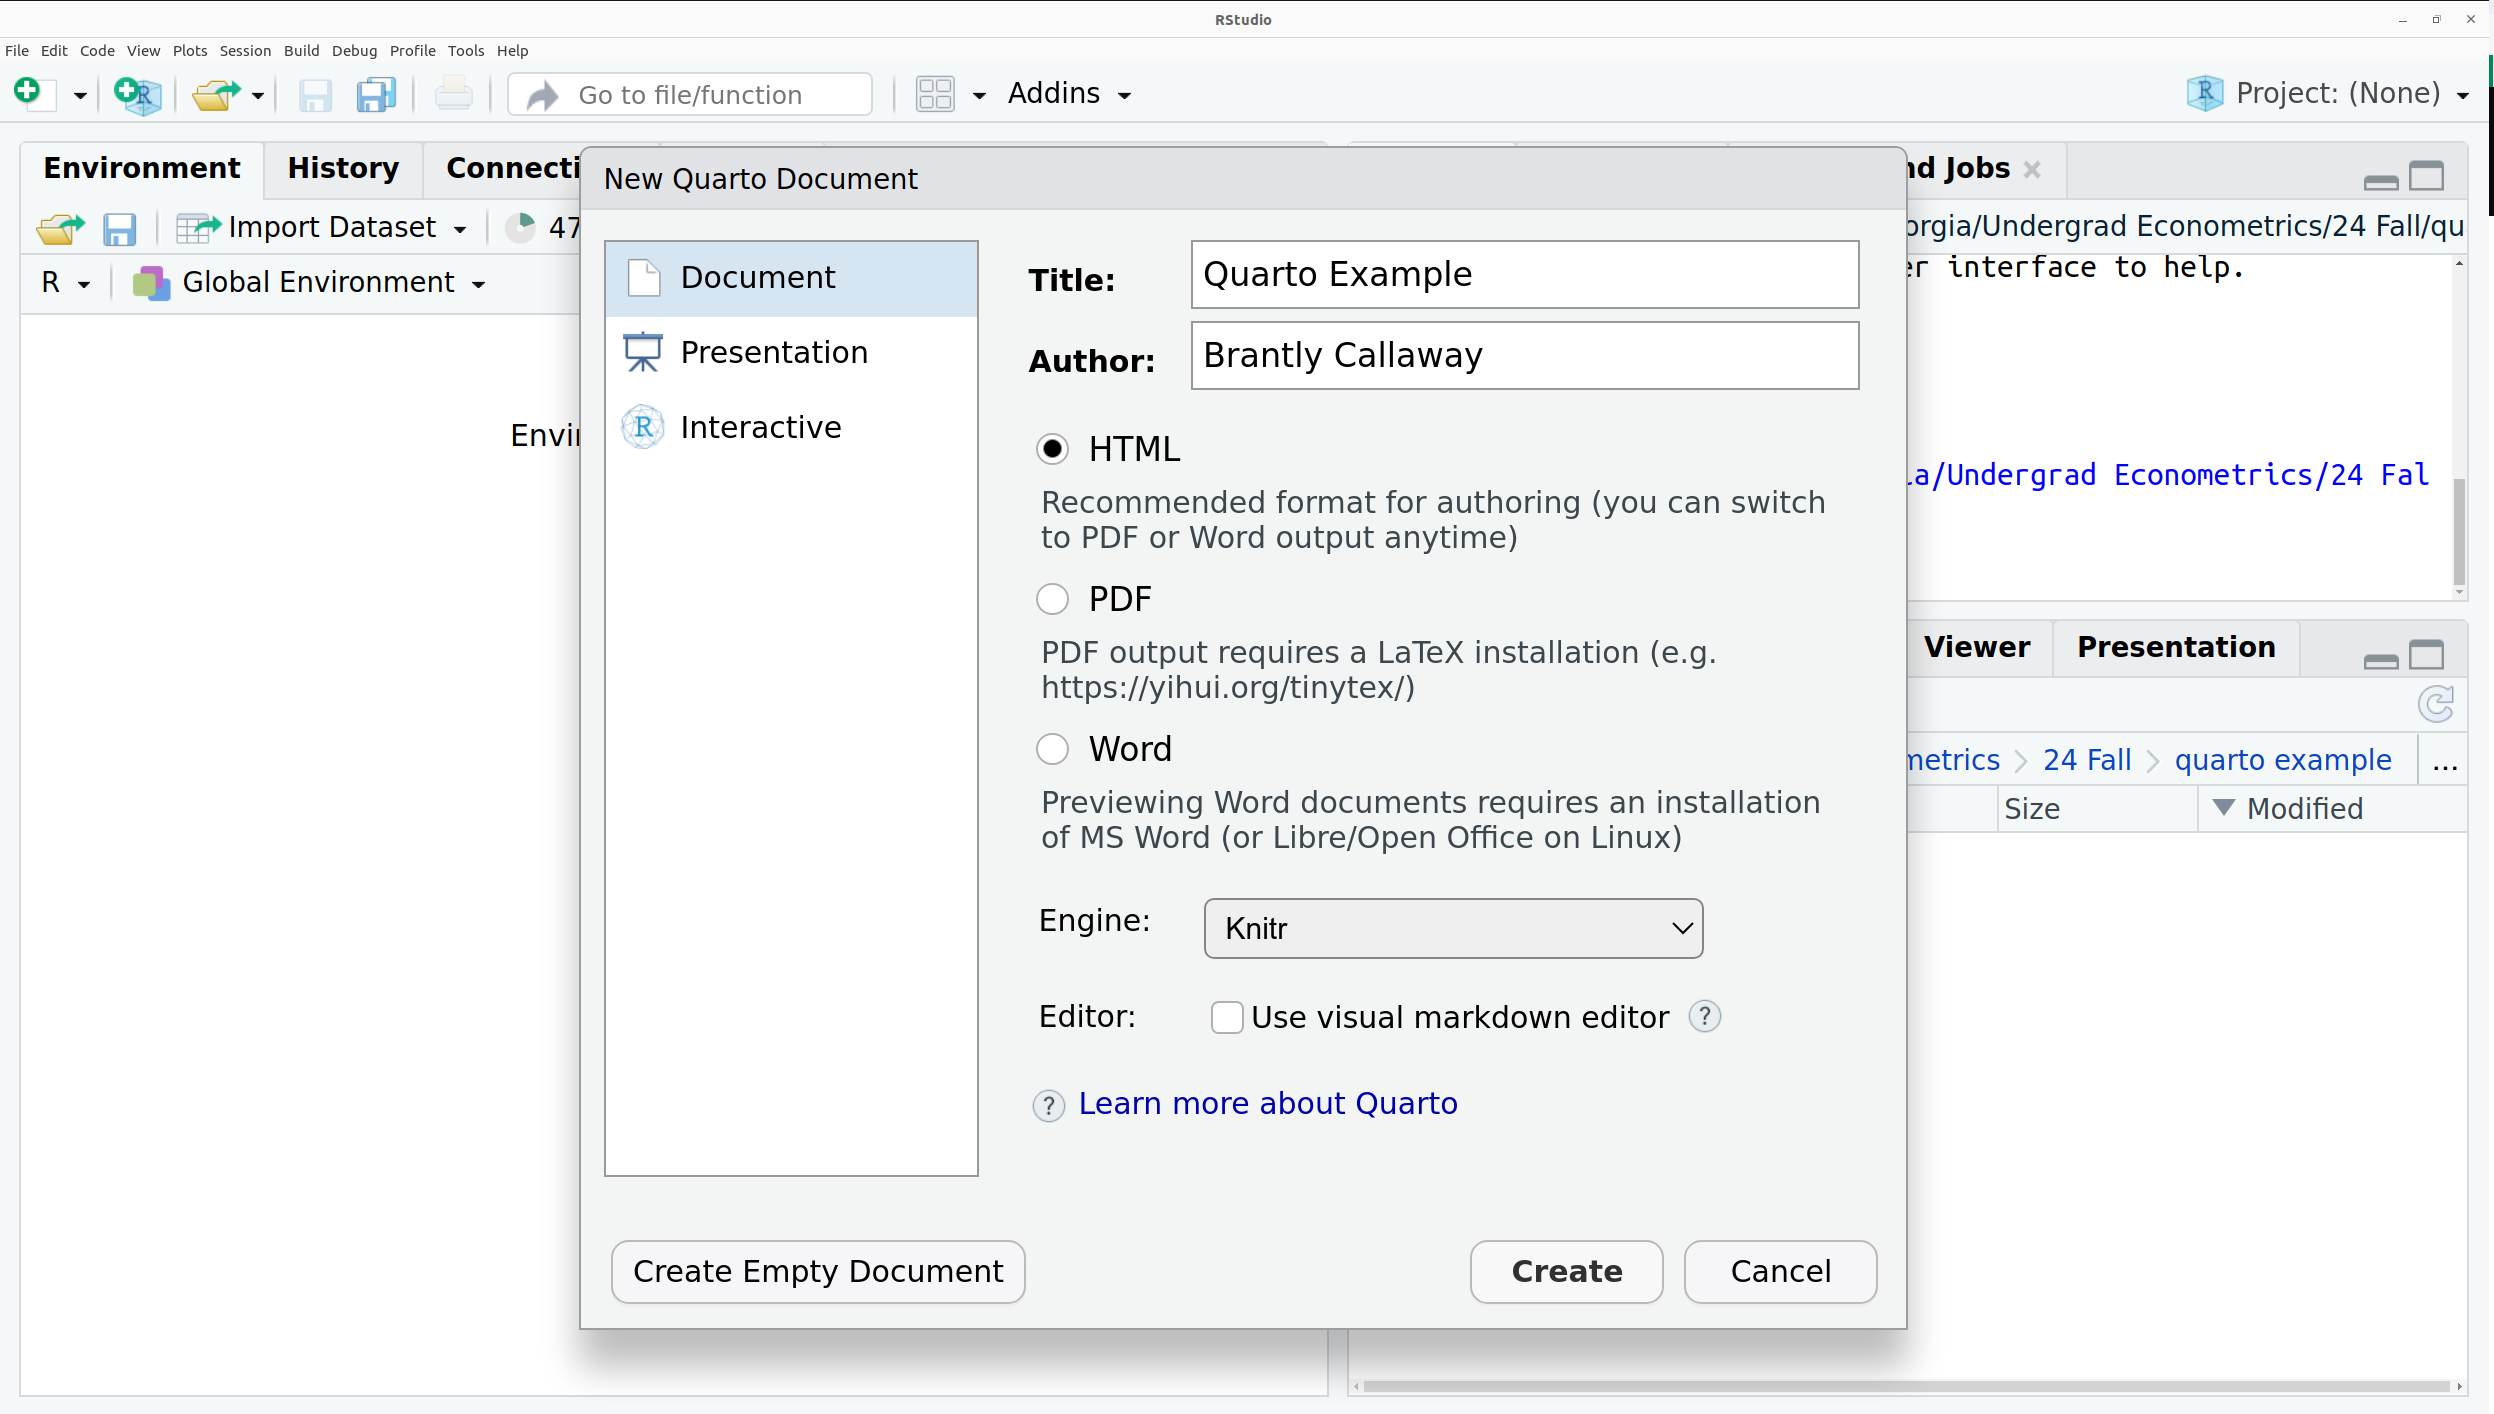
\includegraphics{quarto_setup.png}

You will need to set a few options. I set the title to be
\texttt{Quarto\ Example} and author to be \texttt{Brantly\ Callaway}. I
also unchecked the box at the bottom that says ``Use visual markdown
editor'' {[}I prefer this setting to be unchecked, but you can try it
both ways and see what you like.{]} Now click ``Create'' and your screen
will look something like this

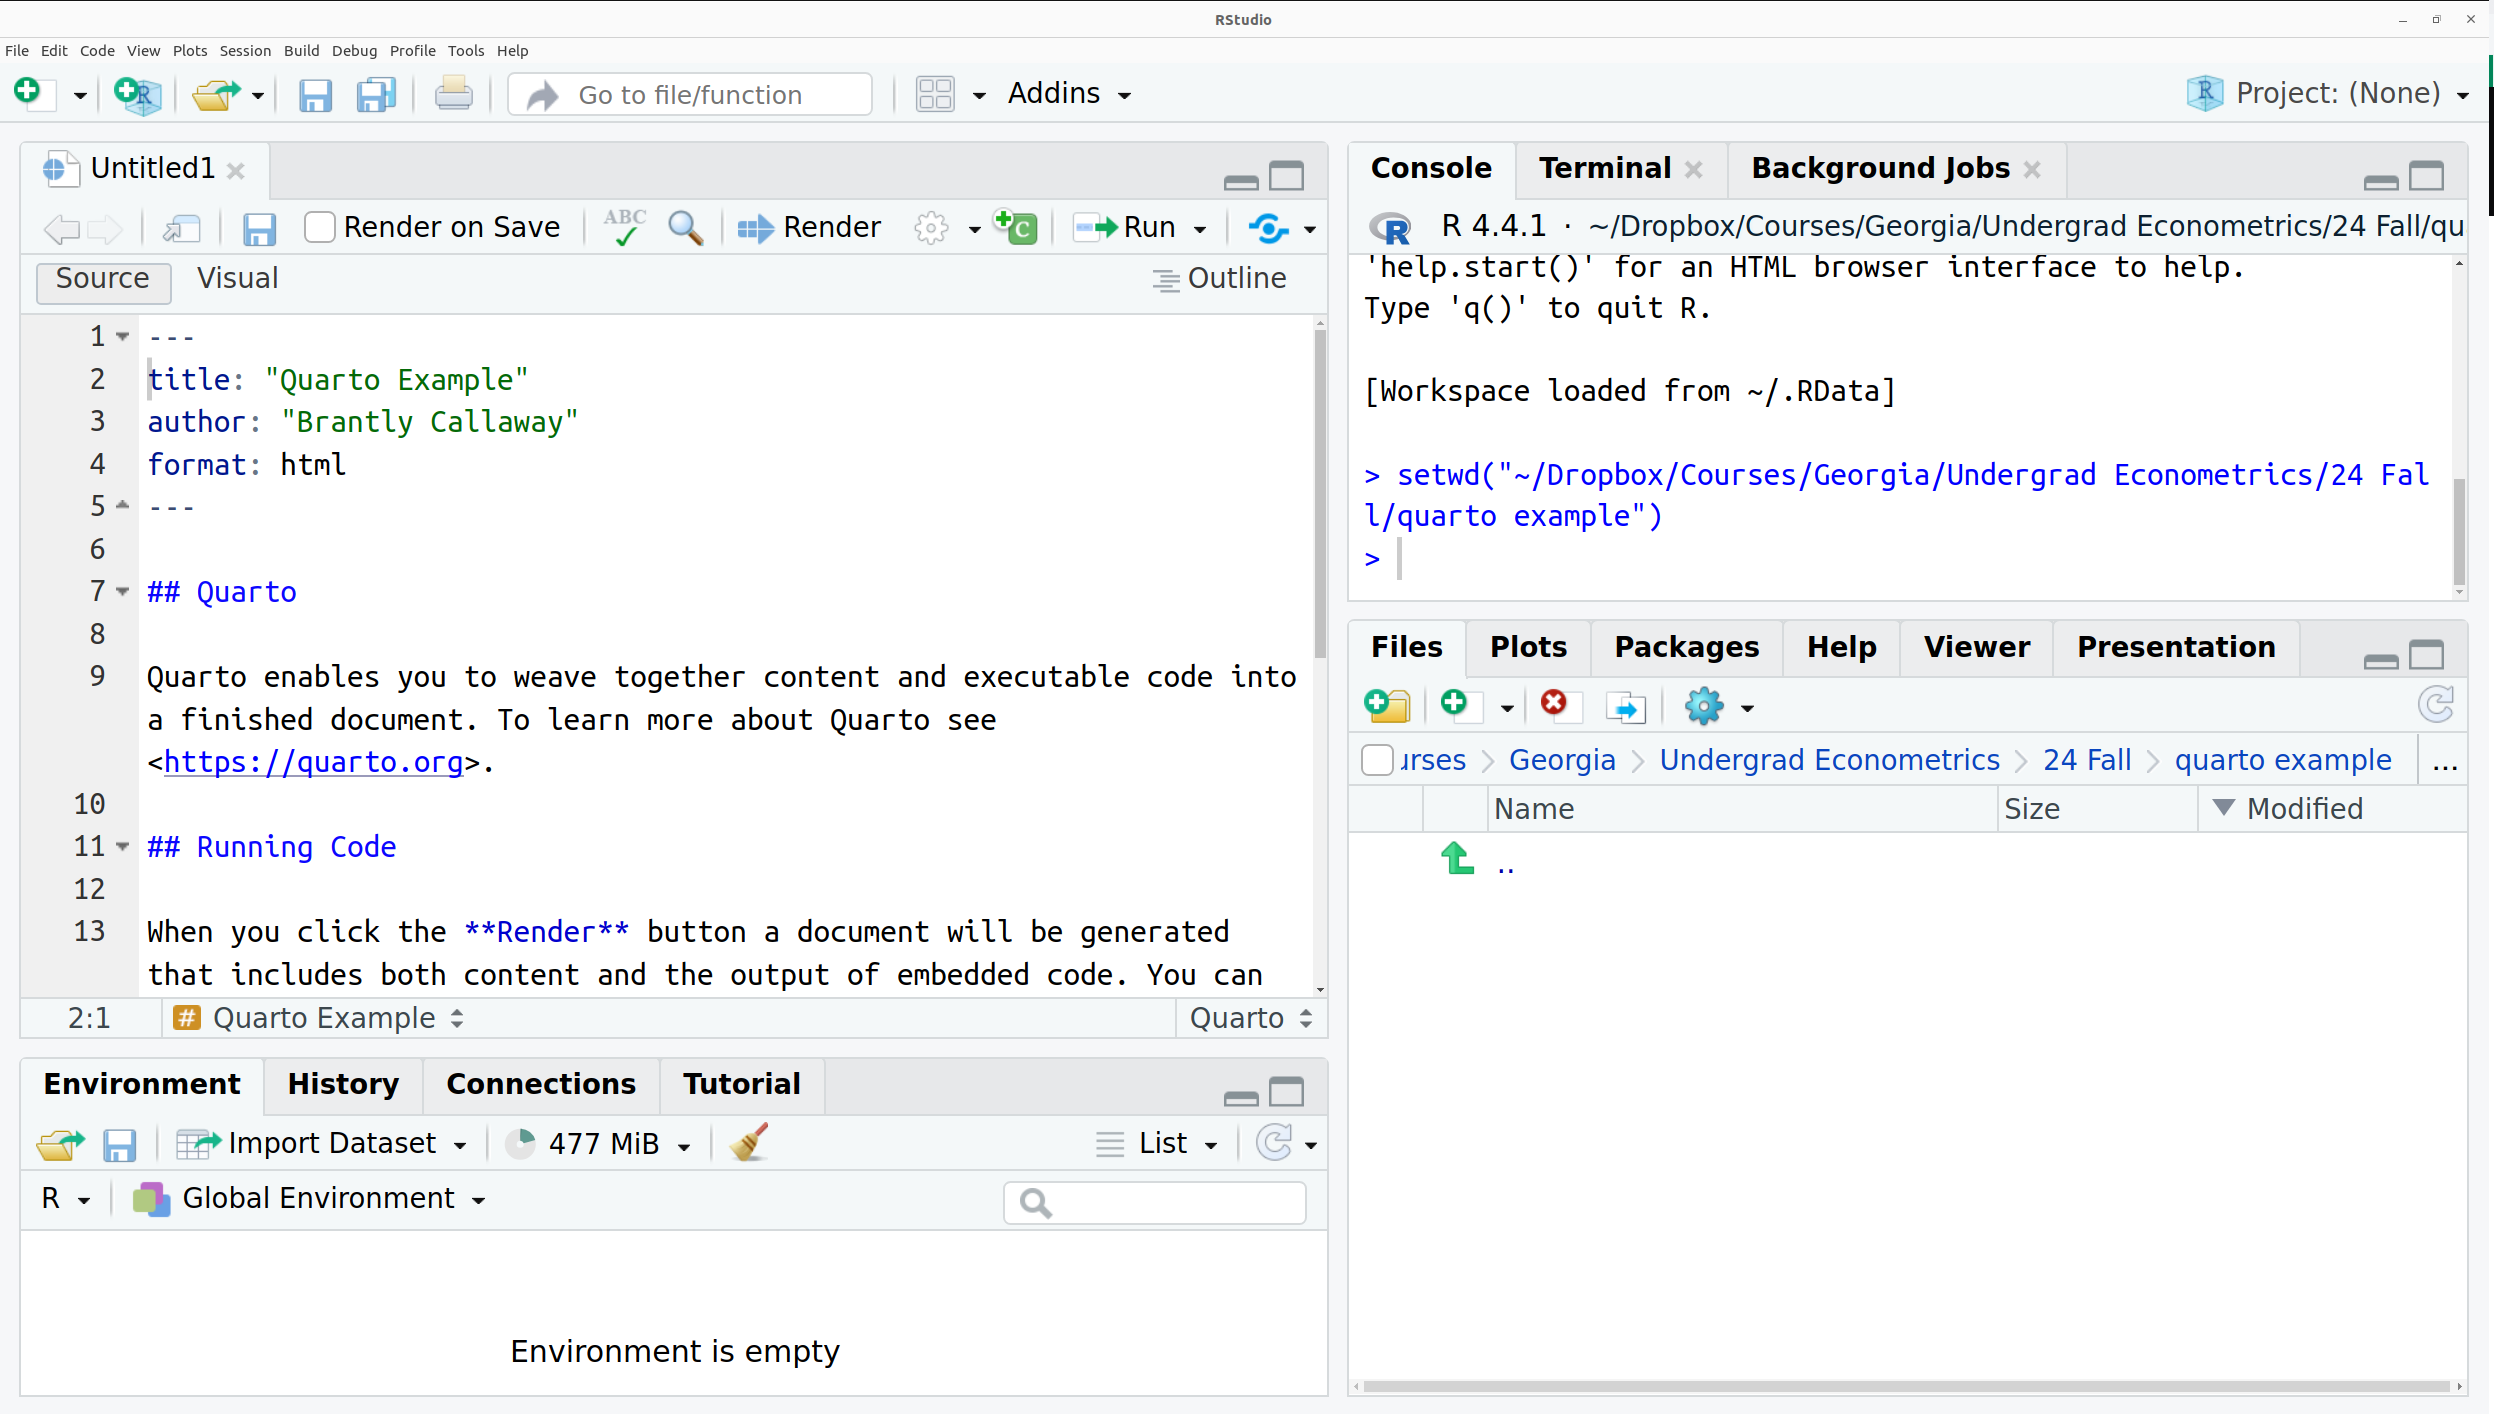
\includegraphics{quarto_file.png}

When you save a Quarto file, you should save it with a \texttt{.qmd}
extension.

Here is a quick example of how you could use Quarto to write homework
solutions. Suppose the first homework of the semester asked you to write
a function called \texttt{sum10} that took in a vector of numbers and
calculated the sum of the first 10 numbers in the vector. Then, report
\texttt{sum10(1:100)}.

\begin{Shaded}
\begin{Highlighting}[]
\SpecialCharTok{{-}{-}{-}}
\NormalTok{title}\SpecialCharTok{:} \StringTok{"Homework 1"}
\NormalTok{author}\SpecialCharTok{:} \StringTok{"Brantly Callaway"}
\NormalTok{format}\SpecialCharTok{:}\NormalTok{ html}
\SpecialCharTok{{-}{-}{-}}

\DocumentationTok{\#\# Question 1}

\NormalTok{To calculate the sum of the first ten numbers }\ControlFlowTok{in}\NormalTok{ a vector, }
\NormalTok{I wrote the following }\ControlFlowTok{function}\SpecialCharTok{:}

\StringTok{\textasciigrave{}\textasciigrave{}\textasciigrave{}}\AttributeTok{\{r\}}
\AttributeTok{sum10 \textless{}{-} function(x) \{}
\AttributeTok{  \# get first 10 elements of x}
\AttributeTok{  x10 \textless{}{-} x[1:10] }
\AttributeTok{  \# calculate their sum and return it}
\AttributeTok{  sum(x10) }
\AttributeTok{\}}

\AttributeTok{sum10(1:100)}
\StringTok{\textasciigrave{}\textasciigrave{}\textasciigrave{}}
\end{Highlighting}
\end{Shaded}

A few last comments for you:

\begin{itemize}
\item
  These notes are written in Quarto, and I write homework solutions in
  Quarto too.
\item
  If you are interested, you can view the source for this book at
  \url{http://github.com/bcallaway11/econ_4750_notes}. The source code
  for this chapter is in the file \texttt{02-programming\_in\_R.qmd}.
\end{itemize}

\section{Advanced Topics}\label{advanced-topics}

To conclude this section, I want to briefly point you towards some
advanced material. We will probably brush up against some of this
material this semester. That being said, R has some very advanced
capabilities related to data science, data manipulation, and data
visualization. If you have time/interest you might push further in all
of these directions. By the end of the semester, we may not have
mastered these topics, but they should at least be accessible to you.

\subsection{Tidyverse}\label{tidyverse}

Related Reading: IDS Chapter 4 --- strongly recommend that you read this

• R has very good data cleaning / manipulating tools

\begin{itemize}
\item
  Many of them are in the
  \href{https://www.tidyverse.org/}{``tidyverse''}
\item
  Mostly this semester, I'll just give you a data set that is ready to
  be worked with. But as you move to your own research projects or do
  work for a company one day, you will realize that a major step in
  analyzing data is organizing (``cleaning'') the data in a way that you
  can analyze it
\end{itemize}

• Main packages

\begin{itemize}
\item
  \texttt{ggplot2} -- see below
\item
  \texttt{dplyr} --- package to manipulate data
\item
  \texttt{tidyr} --- more ways to manipulate data
\item
  \texttt{readr} --- read in data
\item
  \texttt{purrr} --- alternative versions of \texttt{apply} functions
  and \texttt{for} loops
\item
  \texttt{tibble} --- alternative versions of \texttt{data.frame}
\item
  \texttt{stringr} --- tools for working with strings
\item
  \texttt{forcats} --- tools for working with factors
\end{itemize}

• If you see code that uses the pipe operator
\texttt{\%\textgreater{}\%}, it is tidyverse-style code. {[}You need to
load a package to get access to the pipe function. I think this was
introduced in the \texttt{magrittr} package, but you can also load it
with the \texttt{dplyr} package, which is one of the main tidyverse
packages.{]} This is unusual syntax for most programming languages, but
it is (arguably) easier to read. Basically the pipe operator takes the
result from one line of code and ``pipes'' it into the first argument of
the next function. Here is an example

\begin{Shaded}
\begin{Highlighting}[]
\FunctionTok{library}\NormalTok{(dplyr) }\CommentTok{\# or library(magrittr)}
\NormalTok{firm\_data }\SpecialCharTok{\%\textgreater{}\%}
  \FunctionTok{subset}\NormalTok{(employees }\SpecialCharTok{\textgreater{}} \DecValTok{100}\NormalTok{) }\SpecialCharTok{\%\textgreater{}\%}
  \FunctionTok{nrow}\NormalTok{()}
\end{Highlighting}
\end{Shaded}

\begin{verbatim}
[1] 2
\end{verbatim}

What the above code does is it takes the data frame \texttt{firm\_data},
subsets it to firms that have more than 100 rows, and calculates the
number of rows in this subset (i.e., the number of large firms).

It is equivalent to the following, more traditional-looking code:

\begin{Shaded}
\begin{Highlighting}[]
\NormalTok{large\_firms }\OtherTok{\textless{}{-}} \FunctionTok{subset}\NormalTok{(firm\_data, employees }\SpecialCharTok{\textgreater{}} \DecValTok{100}\NormalTok{)}
\FunctionTok{nrow}\NormalTok{(large\_firms)}
\end{Highlighting}
\end{Shaded}

\begin{verbatim}
[1] 2
\end{verbatim}

• I won't emphasize the tidyverse too much as I prefer (at least to some
extent) writing code with a more traditional syntax. That said,
tidyverse packages are really quite useful for data cleaning /
wrangling. And, if you are interested, these are good (and marketable)
skills to have.

\subsection{Data Visualization}\label{data-visualization}

Related Reading: IDS Ch. 6-10 --- \texttt{R} has very good data
visualization tools. I strongly recommend that you read this.

\begin{itemize}
\item
  Another very strong point of \texttt{R}
\item
  Base \texttt{R} comes with the \texttt{plot} command, but the
  \texttt{ggplot2} package provides cutting edge plotting tools. These
  tools will be somewhat harder to learn, but we'll use \texttt{ggplot2}
  this semester as I think it is worth it.
\item
  You can produce professional quality plots in \texttt{R} that are
  publication ready
\end{itemize}

We will use \texttt{ggplot2} this semester, but I will save a longer
discussion for later.

\subsection{Version Control}\label{version-control}

Related Reading: IDS Ch. 19

If you are interested, \href{http://github.com}{GitHub} is a very useful
version control tool (i.e., keeps track of the version of your project,
useful for merging projects, and sharing or co-authoring code) and
\href{http://dropbox.com}{Dropbox} (also useful for sharing code). I use
both of these extensively --- in general, I use GitHub relatively more
for bigger projects and more public projects and Dropbox more for
smaller projects and early versions of projects.

\subsection{RStudio Projects}\label{rstudio-projects}

Related Reading: IDS 20.1

You can create a new project by navigating to
\texttt{File\ -\textgreater{}\ New\ Project}. Projects in RStudio give a
way to organize your, well\ldots{} projects. For this course, you don't
necessarily need to use projects, but you could, for example, create
separate projects for each of your homeworks. This would give you
separate environments for each homework (so you don't have to worry
about accidentally using the same variable name across homeworks leading
to any issues) and a separate set of tabs for scripts in each project.
Your current project is listed in the very top right corner of the
RStudio workspace.

\subsection{Technical Writing Tools}\label{technical-writing-tools}

This is starting to get beyond the scope of the course, but, especially
for students in ECON 6750, I recommend that you look up LaTeX. This is a
markup language mainly for technical, academic writing. The big payoff
is on writing mathematical equations. The equations in the Course Notes
are written in LaTeX. For example, the LaTeX code for the solution to
the quadratic equation written above is

\begin{verbatim}
$$
  x = \frac{-b \pm \sqrt{b^2-4ac}}{2a}
$$
\end{verbatim}

where the \texttt{\$\$} is a delimiter that tells LaTeX to render the
text between the delimiters as an equation,
\texttt{\textbackslash{}frac} is a command that tells LaTeX to render
the text as a fraction, and \texttt{\textbackslash{}pm} is a command
that tells LaTeX to render the text as a plus or minus sign.

As I mentioned above, the course notes are written in \texttt{quarto},
but it is possible to write entire documents in LaTeX. For example, all
of my academic papers are written in pure LaTeX. An easy way to get
started is to use the website \href{http://www.overleaf.com}{Overleaf}.
This is a website that allows you to write LaTeX documents in your web
browser. Writing homework solutions fully in LaTex would be overkill for
this course, but (especially if you are thinking about doing a Ph.D.~in
economics), it would be a good thing to poke around with as you have
time.

\section{Lab 1: Introduction to R
Programming}\label{lab-1-introduction-to-r-programming}

For this lab, we will do several practice problems related to
programming in R.

\begin{enumerate}
\def\labelenumi{\arabic{enumi}.}
\item
  Create two vectors as follows

\begin{Shaded}
\begin{Highlighting}[]
\NormalTok{x }\OtherTok{\textless{}{-}} \FunctionTok{seq}\NormalTok{(}\DecValTok{2}\NormalTok{,}\DecValTok{10}\NormalTok{,}\AttributeTok{by=}\DecValTok{2}\NormalTok{)}
\NormalTok{y }\OtherTok{\textless{}{-}} \FunctionTok{c}\NormalTok{(}\DecValTok{3}\NormalTok{,}\DecValTok{5}\NormalTok{,}\DecValTok{7}\NormalTok{,}\DecValTok{11}\NormalTok{,}\DecValTok{13}\NormalTok{)}
\end{Highlighting}
\end{Shaded}

  Add \texttt{x} and \texttt{y}, subtract \texttt{y} from \texttt{x},
  multiply \texttt{x} and \texttt{y}, and divide \texttt{x} by
  \texttt{y} and report your results.
\item
  The geometric mean of a set of numbers is an alternative measure of
  central tendency to the more common ``arithmetic mean'' (this is the
  mean that we are used to). For a set of \(J\) numbers,
  \(x_1,x_2,\ldots,x_J\), the geometric mean is defined as

  \[
     (x_1 \cdot x_2 \cdot \cdots \cdot x_J)^{1/J}
   \]

  Write a function called \texttt{geometric\_mean} that takes in a
  vector of numbers and computes their geometric mean. Compute the
  geometric mean of \texttt{c(10,8,13)}
\item
  Use the \texttt{lubridate} package to figure out how many days elapsed
  between Jan.~1, 1981 and Jan.~10, 2022.
\item
  \texttt{mtcars} is one of the data frames that comes packaged with
  base R.

  \begin{enumerate}
  \def\labelenumii{\alph{enumii})}
  \item
    How many observations does \texttt{mtcars} have?
  \item
    How many columns does \texttt{mtcars} have?
  \item
    What are the names of the columns of \texttt{mtcars}?
  \item
    Print only the rows of \texttt{mtcars} for cars that get at least 20
    mpg
  \item
    Print only the rows of \texttt{mtcars} that get at least 20 mpg and
    have at least 100 horsepower (it is in the column called
    \texttt{hp})
  \item
    Print only the rows of \texttt{mtcars} that have 6 or more cylinders
    (it is in the column labeld \texttt{cyl}) or at least 100 horsepower
  \item
    Recover the 10th row of \texttt{mtcars}
  \item
    Sort the rows of \texttt{mtcars} by mpg (from highest to lowest)
  \end{enumerate}
\end{enumerate}

\section{Lab 1: Solutions}\label{lab-1-solutions}

1.

\begin{Shaded}
\begin{Highlighting}[]
\NormalTok{x }\OtherTok{\textless{}{-}} \FunctionTok{seq}\NormalTok{(}\DecValTok{2}\NormalTok{,}\DecValTok{10}\NormalTok{,}\AttributeTok{by=}\DecValTok{2}\NormalTok{)}
\NormalTok{y }\OtherTok{\textless{}{-}} \FunctionTok{c}\NormalTok{(}\DecValTok{3}\NormalTok{,}\DecValTok{5}\NormalTok{,}\DecValTok{7}\NormalTok{,}\DecValTok{11}\NormalTok{,}\DecValTok{13}\NormalTok{)}

\NormalTok{x}\SpecialCharTok{+}\NormalTok{y}
\end{Highlighting}
\end{Shaded}

\begin{verbatim}
[1]  5  9 13 19 23
\end{verbatim}

\begin{Shaded}
\begin{Highlighting}[]
\NormalTok{x}\SpecialCharTok{{-}}\NormalTok{y}
\end{Highlighting}
\end{Shaded}

\begin{verbatim}
[1] -1 -1 -1 -3 -3
\end{verbatim}

\begin{Shaded}
\begin{Highlighting}[]
\NormalTok{x}\SpecialCharTok{*}\NormalTok{y}
\end{Highlighting}
\end{Shaded}

\begin{verbatim}
[1]   6  20  42  88 130
\end{verbatim}

\begin{Shaded}
\begin{Highlighting}[]
\NormalTok{x}\SpecialCharTok{/}\NormalTok{y}
\end{Highlighting}
\end{Shaded}

\begin{verbatim}
[1] 0.6666667 0.8000000 0.8571429 0.7272727 0.7692308
\end{verbatim}

2.

\begin{Shaded}
\begin{Highlighting}[]
\NormalTok{geometric\_mean }\OtherTok{\textless{}{-}} \ControlFlowTok{function}\NormalTok{(x) \{}
\NormalTok{  J }\OtherTok{\textless{}{-}} \FunctionTok{length}\NormalTok{(x)}
\NormalTok{  res }\OtherTok{\textless{}{-}} \FunctionTok{prod}\NormalTok{(x)}\SpecialCharTok{\^{}}\NormalTok{(}\DecValTok{1}\SpecialCharTok{/}\NormalTok{J)}
\NormalTok{  res}
\NormalTok{\}}

\FunctionTok{geometric\_mean}\NormalTok{(}\FunctionTok{c}\NormalTok{(}\DecValTok{10}\NormalTok{,}\DecValTok{8}\NormalTok{,}\DecValTok{13}\NormalTok{))}
\end{Highlighting}
\end{Shaded}

\begin{verbatim}
[1] 10.13159
\end{verbatim}

3.

\begin{Shaded}
\begin{Highlighting}[]
\NormalTok{first\_date }\OtherTok{\textless{}{-}}\NormalTok{ lubridate}\SpecialCharTok{::}\FunctionTok{mdy}\NormalTok{(}\StringTok{"01{-}01{-}1981"}\NormalTok{)}
\NormalTok{second\_date }\OtherTok{\textless{}{-}}\NormalTok{ lubridate}\SpecialCharTok{::}\FunctionTok{mdy}\NormalTok{(}\StringTok{"01{-}10{-}2022"}\NormalTok{)}
\NormalTok{second\_date }\SpecialCharTok{{-}}\NormalTok{ first\_date}
\end{Highlighting}
\end{Shaded}

\begin{verbatim}
Time difference of 14984 days
\end{verbatim}

4.

\begin{enumerate}
\def\labelenumi{\alph{enumi})}
\tightlist
\item
\end{enumerate}

\begin{Shaded}
\begin{Highlighting}[]
\FunctionTok{nrow}\NormalTok{(mtcars)}
\end{Highlighting}
\end{Shaded}

\begin{verbatim}
[1] 32
\end{verbatim}

\begin{enumerate}
\def\labelenumi{\alph{enumi})}
\setcounter{enumi}{1}
\tightlist
\item
\end{enumerate}

\begin{Shaded}
\begin{Highlighting}[]
\FunctionTok{ncol}\NormalTok{(mtcars)}
\end{Highlighting}
\end{Shaded}

\begin{verbatim}
[1] 11
\end{verbatim}

\begin{enumerate}
\def\labelenumi{\alph{enumi})}
\setcounter{enumi}{2}
\tightlist
\item
\end{enumerate}

\begin{Shaded}
\begin{Highlighting}[]
\FunctionTok{colnames}\NormalTok{(mtcars)}
\end{Highlighting}
\end{Shaded}

\begin{verbatim}
 [1] "mpg"  "cyl"  "disp" "hp"   "drat" "wt"   "qsec" "vs"   "am"   "gear"
[11] "carb"
\end{verbatim}

\begin{enumerate}
\def\labelenumi{\alph{enumi})}
\setcounter{enumi}{3}
\tightlist
\item
\end{enumerate}

\begin{Shaded}
\begin{Highlighting}[]
\FunctionTok{subset}\NormalTok{(mtcars, mpg }\SpecialCharTok{\textgreater{}=} \DecValTok{20}\NormalTok{)}
\end{Highlighting}
\end{Shaded}

\begin{verbatim}
                mpg cyl  disp  hp drat    wt  qsec vs am gear carb
Mazda RX4      21.0   6 160.0 110 3.90 2.620 16.46  0  1    4    4
Mazda RX4 Wag  21.0   6 160.0 110 3.90 2.875 17.02  0  1    4    4
Datsun 710     22.8   4 108.0  93 3.85 2.320 18.61  1  1    4    1
Hornet 4 Drive 21.4   6 258.0 110 3.08 3.215 19.44  1  0    3    1
Merc 240D      24.4   4 146.7  62 3.69 3.190 20.00  1  0    4    2
Merc 230       22.8   4 140.8  95 3.92 3.150 22.90  1  0    4    2
Fiat 128       32.4   4  78.7  66 4.08 2.200 19.47  1  1    4    1
Honda Civic    30.4   4  75.7  52 4.93 1.615 18.52  1  1    4    2
Toyota Corolla 33.9   4  71.1  65 4.22 1.835 19.90  1  1    4    1
Toyota Corona  21.5   4 120.1  97 3.70 2.465 20.01  1  0    3    1
Fiat X1-9      27.3   4  79.0  66 4.08 1.935 18.90  1  1    4    1
Porsche 914-2  26.0   4 120.3  91 4.43 2.140 16.70  0  1    5    2
Lotus Europa   30.4   4  95.1 113 3.77 1.513 16.90  1  1    5    2
Volvo 142E     21.4   4 121.0 109 4.11 2.780 18.60  1  1    4    2
\end{verbatim}

\begin{enumerate}
\def\labelenumi{\alph{enumi})}
\setcounter{enumi}{4}
\tightlist
\item
\end{enumerate}

\begin{Shaded}
\begin{Highlighting}[]
\FunctionTok{subset}\NormalTok{(mtcars, (mpg }\SpecialCharTok{\textgreater{}=} \DecValTok{20}\NormalTok{) }\SpecialCharTok{\&}\NormalTok{ (hp }\SpecialCharTok{\textgreater{}=} \DecValTok{100}\NormalTok{))}
\end{Highlighting}
\end{Shaded}

\begin{verbatim}
                mpg cyl  disp  hp drat    wt  qsec vs am gear carb
Mazda RX4      21.0   6 160.0 110 3.90 2.620 16.46  0  1    4    4
Mazda RX4 Wag  21.0   6 160.0 110 3.90 2.875 17.02  0  1    4    4
Hornet 4 Drive 21.4   6 258.0 110 3.08 3.215 19.44  1  0    3    1
Lotus Europa   30.4   4  95.1 113 3.77 1.513 16.90  1  1    5    2
Volvo 142E     21.4   4 121.0 109 4.11 2.780 18.60  1  1    4    2
\end{verbatim}

\begin{enumerate}
\def\labelenumi{\alph{enumi})}
\setcounter{enumi}{5}
\tightlist
\item
\end{enumerate}

\begin{Shaded}
\begin{Highlighting}[]
\FunctionTok{subset}\NormalTok{(mtcars, (cyl }\SpecialCharTok{\textgreater{}=} \DecValTok{6}\NormalTok{) }\SpecialCharTok{|}\NormalTok{ (hp }\SpecialCharTok{\textgreater{}=} \DecValTok{100}\NormalTok{))}
\end{Highlighting}
\end{Shaded}

\begin{verbatim}
                     mpg cyl  disp  hp drat    wt  qsec vs am gear carb
Mazda RX4           21.0   6 160.0 110 3.90 2.620 16.46  0  1    4    4
Mazda RX4 Wag       21.0   6 160.0 110 3.90 2.875 17.02  0  1    4    4
Hornet 4 Drive      21.4   6 258.0 110 3.08 3.215 19.44  1  0    3    1
Hornet Sportabout   18.7   8 360.0 175 3.15 3.440 17.02  0  0    3    2
Valiant             18.1   6 225.0 105 2.76 3.460 20.22  1  0    3    1
Duster 360          14.3   8 360.0 245 3.21 3.570 15.84  0  0    3    4
Merc 280            19.2   6 167.6 123 3.92 3.440 18.30  1  0    4    4
Merc 280C           17.8   6 167.6 123 3.92 3.440 18.90  1  0    4    4
Merc 450SE          16.4   8 275.8 180 3.07 4.070 17.40  0  0    3    3
Merc 450SL          17.3   8 275.8 180 3.07 3.730 17.60  0  0    3    3
Merc 450SLC         15.2   8 275.8 180 3.07 3.780 18.00  0  0    3    3
Cadillac Fleetwood  10.4   8 472.0 205 2.93 5.250 17.98  0  0    3    4
Lincoln Continental 10.4   8 460.0 215 3.00 5.424 17.82  0  0    3    4
Chrysler Imperial   14.7   8 440.0 230 3.23 5.345 17.42  0  0    3    4
Dodge Challenger    15.5   8 318.0 150 2.76 3.520 16.87  0  0    3    2
AMC Javelin         15.2   8 304.0 150 3.15 3.435 17.30  0  0    3    2
Camaro Z28          13.3   8 350.0 245 3.73 3.840 15.41  0  0    3    4
Pontiac Firebird    19.2   8 400.0 175 3.08 3.845 17.05  0  0    3    2
Lotus Europa        30.4   4  95.1 113 3.77 1.513 16.90  1  1    5    2
Ford Pantera L      15.8   8 351.0 264 4.22 3.170 14.50  0  1    5    4
Ferrari Dino        19.7   6 145.0 175 3.62 2.770 15.50  0  1    5    6
Maserati Bora       15.0   8 301.0 335 3.54 3.570 14.60  0  1    5    8
Volvo 142E          21.4   4 121.0 109 4.11 2.780 18.60  1  1    4    2
\end{verbatim}

\begin{enumerate}
\def\labelenumi{\alph{enumi})}
\setcounter{enumi}{6}
\tightlist
\item
\end{enumerate}

\begin{Shaded}
\begin{Highlighting}[]
\NormalTok{mtcars[}\DecValTok{10}\NormalTok{,]}
\end{Highlighting}
\end{Shaded}

\begin{verbatim}
          mpg cyl  disp  hp drat   wt qsec vs am gear carb
Merc 280 19.2   6 167.6 123 3.92 3.44 18.3  1  0    4    4
\end{verbatim}

\begin{enumerate}
\def\labelenumi{\alph{enumi})}
\setcounter{enumi}{7}
\tightlist
\item
\end{enumerate}

\begin{Shaded}
\begin{Highlighting}[]
\CommentTok{\# without reversing the order, we would order from lowest to smallest}
\NormalTok{mtcars[}\FunctionTok{rev}\NormalTok{(}\FunctionTok{order}\NormalTok{(mtcars}\SpecialCharTok{$}\NormalTok{mpg)),]}
\end{Highlighting}
\end{Shaded}

\begin{verbatim}
                     mpg cyl  disp  hp drat    wt  qsec vs am gear carb
Toyota Corolla      33.9   4  71.1  65 4.22 1.835 19.90  1  1    4    1
Fiat 128            32.4   4  78.7  66 4.08 2.200 19.47  1  1    4    1
Lotus Europa        30.4   4  95.1 113 3.77 1.513 16.90  1  1    5    2
Honda Civic         30.4   4  75.7  52 4.93 1.615 18.52  1  1    4    2
Fiat X1-9           27.3   4  79.0  66 4.08 1.935 18.90  1  1    4    1
Porsche 914-2       26.0   4 120.3  91 4.43 2.140 16.70  0  1    5    2
Merc 240D           24.4   4 146.7  62 3.69 3.190 20.00  1  0    4    2
Merc 230            22.8   4 140.8  95 3.92 3.150 22.90  1  0    4    2
Datsun 710          22.8   4 108.0  93 3.85 2.320 18.61  1  1    4    1
Toyota Corona       21.5   4 120.1  97 3.70 2.465 20.01  1  0    3    1
Volvo 142E          21.4   4 121.0 109 4.11 2.780 18.60  1  1    4    2
Hornet 4 Drive      21.4   6 258.0 110 3.08 3.215 19.44  1  0    3    1
Mazda RX4 Wag       21.0   6 160.0 110 3.90 2.875 17.02  0  1    4    4
Mazda RX4           21.0   6 160.0 110 3.90 2.620 16.46  0  1    4    4
Ferrari Dino        19.7   6 145.0 175 3.62 2.770 15.50  0  1    5    6
Pontiac Firebird    19.2   8 400.0 175 3.08 3.845 17.05  0  0    3    2
Merc 280            19.2   6 167.6 123 3.92 3.440 18.30  1  0    4    4
Hornet Sportabout   18.7   8 360.0 175 3.15 3.440 17.02  0  0    3    2
Valiant             18.1   6 225.0 105 2.76 3.460 20.22  1  0    3    1
Merc 280C           17.8   6 167.6 123 3.92 3.440 18.90  1  0    4    4
Merc 450SL          17.3   8 275.8 180 3.07 3.730 17.60  0  0    3    3
Merc 450SE          16.4   8 275.8 180 3.07 4.070 17.40  0  0    3    3
Ford Pantera L      15.8   8 351.0 264 4.22 3.170 14.50  0  1    5    4
Dodge Challenger    15.5   8 318.0 150 2.76 3.520 16.87  0  0    3    2
AMC Javelin         15.2   8 304.0 150 3.15 3.435 17.30  0  0    3    2
Merc 450SLC         15.2   8 275.8 180 3.07 3.780 18.00  0  0    3    3
Maserati Bora       15.0   8 301.0 335 3.54 3.570 14.60  0  1    5    8
Chrysler Imperial   14.7   8 440.0 230 3.23 5.345 17.42  0  0    3    4
Duster 360          14.3   8 360.0 245 3.21 3.570 15.84  0  0    3    4
Camaro Z28          13.3   8 350.0 245 3.73 3.840 15.41  0  0    3    4
Lincoln Continental 10.4   8 460.0 215 3.00 5.424 17.82  0  0    3    4
Cadillac Fleetwood  10.4   8 472.0 205 2.93 5.250 17.98  0  0    3    4
\end{verbatim}

\section{Coding Exercises}\label{coding-exercises}

\begin{enumerate}
\def\labelenumi{\arabic{enumi}.}
\item
  The \texttt{stringr} package contains a number of functions for
  working with strings. For this problem create the following character
  vector in R

\begin{Shaded}
\begin{Highlighting}[]
\NormalTok{x }\OtherTok{\textless{}{-}} \FunctionTok{c}\NormalTok{(}\StringTok{"economics"}\NormalTok{, }\StringTok{"econometrics"}\NormalTok{, }\StringTok{"ECON 4750"}\NormalTok{)}
\end{Highlighting}
\end{Shaded}

  Install the \texttt{stringr} package and use the \texttt{str\_length}
  function in the package in order to calculate the length (number of
  characters) in each element of \texttt{x}.
\item
  For this problem, we are going to write a function to calculate the
  sum of the numbers from 1 to \(n\) where \(n\) is some positive
  integer. There are actually a lot of different ways to do this.

  \begin{itemize}
  \item
    Approach 1: write a function called \texttt{sum\_one\_to\_n\_1} that
    uses the R functions \texttt{seq} to create a list of numbers from 1
    to \(n\) and then the function \texttt{sum} to sum over that list.
  \item
    Approach 2: The sum of numbers from 1 to \(n\) is equal to
    \(n(n+1)/2\). Use this expression to write a function called
    \texttt{sum\_one\_to\_n\_2} to calculate the sum from 1 to \(n\).\\
  \item
    Approach 3: A more brute force approach is to create a list of
    numbers from 1 to \(n\) (you can use \texttt{seq} here) and add them
    up using a \texttt{for} loop --- basically, just keep track of what
    the current total is and add the next number to the total in each
    iteration of the for loop. Write a function called
    \texttt{sum\_one\_to\_n\_3} that does this.
  \end{itemize}

  \textbf{Hint:} All of the functions should look like

\begin{Shaded}
\begin{Highlighting}[]
\NormalTok{sum\_one\_to\_n }\OtherTok{\textless{}{-}} \ControlFlowTok{function}\NormalTok{(n) \{}
  \CommentTok{\# do something}
\NormalTok{\}}
\end{Highlighting}
\end{Shaded}

  Try out all three approaches that you came up with above for
  \(n=100\). What is the answer? Do you get the same answer using all
  three approaches?
\item
  The Fibonacci sequence is the sequence of numbers
  \(0,1,1,2,3,5,8,13,21,34,55,\ldots\) that comes from starting with
  \(0\) and \(1\) and where each subsequent number is the sum of the
  previous two. For example, the 5 in the sequence comes from adding 2
  and 3; the 55 in the sequence comes from adding 21 and 34.

  \begin{enumerate}
  \def\labelenumii{\alph{enumii})}
  \item
    Write a function called \texttt{fibonacci} that takes in a number
    \texttt{n} and computes the nth element in the Fibonacci sequence.
    For example \texttt{fibonacci(5)} should return \texttt{3} and
    \texttt{fibonacci(8)} should return \texttt{13}.
  \item
    Consider an alternative sequence where, starting with the third
    element, each element is computed as the sum of the previous two
    elements (the same as with the Fibonacci sequence) but where the
    first two elements can be arbitrary. Write a function
    \texttt{alt\_seq(a,b,n)} where \texttt{a} is the first element in
    the sequence, \texttt{b} is the second element in the sequence, and
    \texttt{n} is which element in the sequence to return. For example,
    if \(a=3\) and \(b=7\), then the sequence would be
    \(3,7,10,17,27,44,71,\ldots\) and
    \texttt{alt\_seq(a=3,b=7,n=4)\ =\ 17}.
  \end{enumerate}
\item
  This problem involves writing functions related to computing prime
  numbers. Recall that a prime number is a positive integer whose only
  (integer) factors are 1 and itself (e.g., \(6\) is not prime because
  it factors into \(2\times 3\), but \(5\) is a prime number because its
  only factors are \(1\) and \(5\)).

  For this problem, you cannot use any built-in functions in \texttt{R}
  for computing prime numbers or checking whether or not a number is a
  prime number. However, a helpful function for this problem is the
  \emph{modulo} function, \texttt{\%\%} discussed earlier in the notes.
  \textbf{Hint:} Notice that \texttt{6\ \%\%\ 2\ =\ 0} indicates that
  \texttt{2} is a factor of \texttt{6}; on the other hand, if you divide
  \(5\) by any integer small than itself (except for \(1\)), the
  remainder will always be non-zero.

  \begin{enumerate}
  \def\labelenumii{\alph{enumii})}
  \item
    Write a function \texttt{is\_prime} that takes \texttt{x} as an
    argument and returns \texttt{TRUE} if \texttt{x} is a prime number
    and returns \texttt{FALSE} if \texttt{x} is not a prime number.
  \item
    Write a function \texttt{prime} that takes \texttt{n} as an argument
    and returns a vector of all the prime numbers from \(1\) to \(n\).
    If it is helpful, \texttt{prime} can call the function
    \texttt{is\_prime} that you wrote for part (a).
  \end{enumerate}
\item
  Base \texttt{R} includes a data frame called \texttt{iris}. This is
  data about iris flowers (you can read the details by running
  \texttt{?iris}).

  \begin{enumerate}
  \def\labelenumii{\alph{enumii})}
  \item
    How many observations are there in the entire data frame?
  \item
    Calculate the average \texttt{Sepal.Length} across all observations
    in \texttt{iris}.
  \item
    Calculate the average \texttt{Sepal.Width} among the \texttt{setosa}
    iris species.
  \item
    Sort \texttt{iris} by \texttt{Petal.Length} and print the first 10
    rows.
  \end{enumerate}
\item
  One of the examples that we gave above was about writing a function to
  solve quadratic equations, but, in the code presented above, we only
  returned one solution to the quadratic equation. Write a function
  \texttt{quadratic\_solver} that takes in \texttt{a}, \texttt{b}, and
  \texttt{c} as arguments and returns both solutions to the quadratic
  equation in a list. For example, \texttt{quadratic\_solver(1,4,3)}
  should return a list with two elements, \texttt{-1} and \texttt{-3}.
\end{enumerate}

\part{Probability}

\bookmarksetup{startatroot}

\chapter{Random Variables}\label{random-variables}

\[
\newcommand{\E}{\mathbb{E}}
\renewcommand{\P}{\textrm{P}}
\let\L\relax
\newcommand{\L}{\textrm{L}} %doesn't work in .qmd, place this command at start of qmd file to use it
\newcommand{\F}{\textrm{F}}
\newcommand{\var}{\textrm{var}}
\newcommand{\cov}{\textrm{cov}}
\newcommand{\corr}{\textrm{corr}}
\newcommand{\Var}{\mathrm{Var}}
\newcommand{\Cov}{\mathrm{Cov}}
\newcommand{\Corr}{\mathrm{Corr}}
\newcommand{\sd}{\mathrm{sd}}
\newcommand{\se}{\mathrm{s.e.}}
\newcommand{\T}{T}
\newcommand{\indicator}[1]{\mathbb{1}\{#1\}}
\newcommand\independent{\perp \!\!\! \perp}
\newcommand{\N}{\mathcal{N}}
\]

This section contains our crash course review of topics in probability.
The discussion mostly follows Chapter 2 in the Stock and Watson
textbook, and I have cross-listed the relevant sections in the textbook
here.

At a very high level, probability is the set of mathematical tools that
allow us to think about \textbf{random} events.

Just to be clear, random means \emph{uncertain}, not 50:50.

A simple example of a random event is the outcome from rolling a die.

Eventually, we will treat data as being random draws from some
population. Examples of things that we will treat as random draws are
things like a person's hair color, height, income, etc. We will think of
all of these as being random draws because \emph{ex ante} we don't know
what they will be.

\section{Data for this chapter}\label{data-for-this-chapter}

For this chapter, we'll use data from the U.S. Census Bureau from 2019.
It is not quite a full census, but we'll treat it as the population
throughout this chapter.

\section{Random Variables}\label{random-variables-1}

SW 2.1

A \textbf{random variable} is a numerical summary of some random event.

Some examples:

\begin{itemize}
\item
  Outcome of roll of a die
\item
  A person's height in inches
\item
  A firm's profits in a particular year
\item
  Creating a random variable sometime involves ``coding'' non-numeric
  outcomes, e.g., setting \texttt{hair=1} if a person's hair color is
  black, \texttt{hair=2} if a person's hair is blonde, etc.
\end{itemize}

We'll generally classify random variables into one of two categories

\begin{itemize}
\item
  \textbf{Discrete} --- A random variable that takes on discrete values
  such as 0, 1, 2
\item
  \textbf{Continuous} --- Takes on a continuum of values
\end{itemize}

These are broad categories because a lot of random variables in
economics sit in between these two.

\section{pdfs, pmfs, and cdfs}\label{pdfs-pmfs-and-cdfs}

SW 2.1

The \textbf{distribution} of a random variable describes how likely it
is take on certain values.

A random variable's distribution is fully summarized by its:

\begin{itemize}
\item
  \textbf{probability mass function (pmf)} if the random variable is
  discrete
\item
  \textbf{probability density function (pdf)} if the random variable is
  continuous
\end{itemize}

The pmf is somewhat easier to explain, so let's start there. For some
discrete random variable \(X\), its pmf is given by

\[
  f_X(x) = \P(X=x)
\] That is, the probability that \(X\) takes on some particular value
\(x\).

{Example: } Suppose that \(X\) denotes the outcome of a roll of a die.
Then, \(f_X(1)\) is the probability of rolling a one. And, in
particular,

\[
  f_X(1) = \P(X=1) = \frac{1}{6}
\]

{Example: } Let's do a bit more realistic example where we look at the
pmf of education in the U.S. Suppose that \(X\) denotes the years of
education that a person has. Then, \(f_X(x)\) is the probability that a
person has exactly \(x\) years of education. We can set \(x\) to
different values and calculate the probabilities of a person having
different amounts of education. That's what we do in the following
figure:

\begin{figure}[H]

{\centering 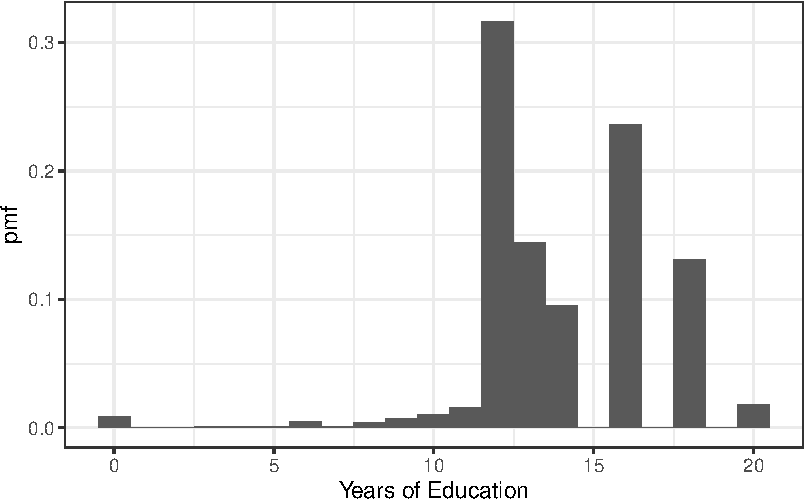
\includegraphics{03-random_variables_files/figure-pdf/unnamed-chunk-3-1.pdf}

}

\caption{pmf of U.S. education}

\end{figure}%

There are some things that are perhaps worth pointing out here. The most
common amount of education in the U.S. appears to be exactly 12 years
--- corresponding to graduating from high school; about 32\% of the
population has that level of education. The next most common number of
years of education is 16 --- corresponding to graduating from college;
about 24\% of individuals have this level of education. Other relatively
common values of education are 13 years (14\% of individuals) and 18
(13\% of individuals). About 1\% of individuals report 0 years of
education. It's not clear to me whether or not that is actually true or
reflects some individuals mis-reporting their education.

Before going back to the pdf, let me describe another way to fully
summarize the distribution of a random variable.

\begin{itemize}
\tightlist
\item
  \textbf{Cumulative distribution function (cdf)} - The cdf of some
  random variable \(X\) is defined as
\end{itemize}

\[
  F_X(x) = \P(X \leq x)
\] In words, this cdf is the probability that the random \(X\) takes a
value less than or equal to \(x\).

{Example: } Suppose \(X\) is the outcome of a roll of a die. Then,
\(F_X(3) = \P(X \leq 3)\) is the probability of rolling 3 or lower.
Thus,

\[
  F_X(3) = \P(X \leq 3) = \frac{1}{2}
\]

{Example: } Let's go back to our example of years of education in the
U.S. In this case, \(F_X(x)\) is the fraction of the population that has
less than \(x\) years of education. We can calculate this for different
values of \(x\). That's what we do in the following figure:

\begin{figure}[H]

{\centering 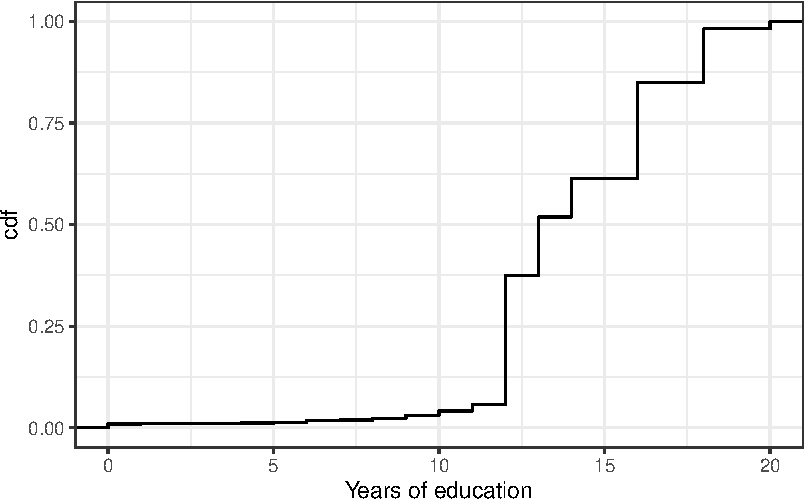
\includegraphics{03-random_variables_files/figure-pdf/unnamed-chunk-4-1.pdf}

}

\caption{cdf of U.S. educ}

\end{figure}%

You can see that the cdf is increasing in the years of education. And
there are big ``jumps'' in the cdf at values of years of education that
are common such as 12 and 16.

We'll go over some properties of pmfs and cdfs momentarily (perhaps you
can already deduce some of them from the above figures), but before we
do that, we need to go over some (perhaps new) tools.

\section{Summation operator}\label{summation-operator}

It will be convenient for us to have a notation that allows us to add up
many numbers/variables at the same time. To do this, we'll introduce the
\(\sum\) operation.

As a simple example, suppose that we have three variables (it doesn't
matter if they are random or not): \(x_1,x_2,x_3\) and we want to add
them up. Then, we can write \[
  \sum_{i=1}^3 x_i := x_1 + x_2 + x_3
\] Many times, once we have data, there will be n ``observations'' and
we can add them up by: \[
  \sum_{i=1}^n x_i = x_1 + x_2 + \cdots + x_n
\] \textbf{Properties:}

\begin{enumerate}
\def\labelenumi{\arabic{enumi}.}
\item
  For any constant \(c\),

  \[
   \sum_{i=1}^n c = n \cdot c
   \]

  {[}This is just the definition of multiplication{]}
\item
  For any constant c,

  \[
     \sum_{i=1}^n c x_i = c \sum_{i=1}^n x_i
   \]

  In words: constants can be moved out of the summation.

  We will use the property often throughout the semester.

  As an example,

  \[
     \begin{aligned}
     \sum_{i=1}^3 7 x_i &= 7x_1 + 7x_2 + 7x_3 \\
     &= 7(x_1 + x_2 + x_3) \\
     &= 7 \sum_{i=1}^3 x_i
     \end{aligned}
   \]

  where the first line is just the definition of the summation, the
  second equality factors out the 7, and the last equality writes the
  part about adding up the \(x\)'s using summation notation.
\end{enumerate}

\section{Properties of pmfs and cdfs}\label{properties-of-pmfs-and-cdfs}

Let's define the \textbf{support} of a random variable \(X\) --- this is
the set of all possible values that \(X\) can possibly take. We'll use
the notation \(\mathcal{X}\) to denote the support of \(X\).

{Example: }Suppose \(X\) is the outcome from a roll of a die. Then, the
support of \(X\) is given by \(\mathcal{X} = \{1,2,3,4,5,6\}\). In other
words, the only possible values for \(X\) are from \(1,\ldots,6\).

{Example: }Suppose \(X\) is the number of years of education that a
person has. The support of \(X\) is given by
\(\mathcal{X} = \{0, 1, 2, \ldots, 20\}\). Perhaps I should have chosen
a larger number than 20 to be the maximum possible value that \(X\)
could take, but you will get the idea --- a person's years of education
can be 0 or 1 or 2 or up to some maximum value.

\textbf{Properties of pmfs}

\begin{enumerate}
\def\labelenumi{\arabic{enumi}.}
\item
  For any \(x\), \(0 \leq f_X(x) \leq 1\)

  In words: the probability of \(X\) taking some particular value can't
  be less than 0 or greater than 1 (neither of those would make any
  sense)
\item
  \(\sum_{x \in \mathcal{X}} f_X(x) = 1\)

  In words: if you add up \(\P(X=x)\) across all possible values that
  \(X\) could take, they sum to 1.
\end{enumerate}

\textbf{Properties of cdfs for discrete random variables}

\begin{enumerate}
\def\labelenumi{\arabic{enumi}.}
\item
  For any \(x\), \(0 \leq F_X(x) \leq 1\)

  In words: the probability that \(X\) is less than or equal to some
  particular value \(x\) has to be between 0 and 1.
\item
  If \(x_1 < x_2\), then \(F_X(x_1) \leq F_X(x_2)\)

  In words: the cdf is increasing in \(x\) (e.g., it will always be the
  case that \(\P(X \leq 3) \leq \P(X \leq 4)\)).
\item
  \(F_X(-\infty)=0\) and \(F_X(\infty)=1\)

  In words: if you choose small enough values of \(x\), the probability
  that \(X\) will be less than that is 0; similar (but opposite) logic
  applies for big values of \(x\).
\end{enumerate}

\textbf{Connection between pmfs and cdfs}

\begin{enumerate}
\def\labelenumi{\arabic{enumi}.}
\item
  \(F_X(x) = \displaystyle \sum_{z \in \mathcal{X} \\ z \leq x} f_X(z)\)

  In words: you can ``recover'' the cdf from the pmf by adding up the
  pmf across all possible values that the random variable could take
  that are less than or equal to \(x\). This will be clearer with an
  example:
\end{enumerate}

{Example: }Suppose that \(X\) is the outcome of a roll of a die. Earlier
we showed that \(F_X(3) = 1/2\). We can calculate this by

\[
  \begin{aligned}
  F_X(3) &= \sum_{\substack{z \in \mathcal{X} \\ z \leq 3}} f_X(z) \\
  &= \sum_{z=1}^3 f_X(z) \\
  &= f_X(1) + f_X(2) + f_X(3) \\
  &= \frac{1}{6} + \frac{1}{6} + \frac{1}{6} \\
  &= \frac{1}{2}
  \end{aligned}
\]

\section{Continuous Random Variables}\label{continuous-random-variables}

SW 2.1

For continuous random variables, you can define the cdf in exactly the
same way as we did for discrete random variables. That is, if \(X\) is a
continuous random variable,

\[
  F_X(x) = \P(X \leq x)
\]

{Example: } Suppose \(X\) denotes an individual's yearly wage income.
The cdf of \(X\) looks like

\begin{figure}[H]

{\centering 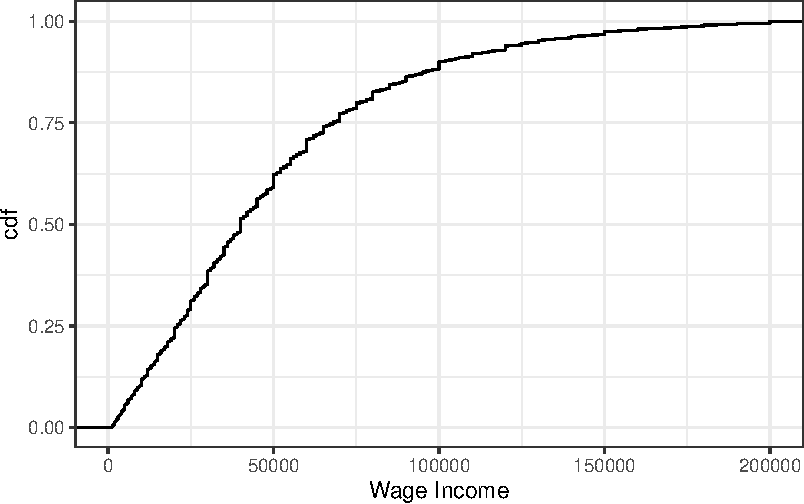
\includegraphics{03-random_variables_files/figure-pdf/unnamed-chunk-5-1.pdf}

}

\caption{cdf of U.S. wage income}

\end{figure}%

From the figure, we can see that about 24\% of working individuals in
the U.S. each \$20,000 or less per year, 61\% of working individuals
earn \$50,000 or less, and 88\% earn \$100,000 or less.

It's trickier to define an analogue to the pmf for a continuous random
variable (in fact, this is the main reason for our separate treatment of
discrete and continuous random variables). For example, suppose \(X\)
denotes the length of a phone conversation. As long as we can measure
time finely enough, the probability that a phone conversation lasts
exactly 1189.23975381 seconds (this is about 20 minutes) is 0. Instead,
for a continuous random variable, we'll define its probability density
function (pdf) as the derivative of its cdf, that is,

\[
  f_X(x) := \frac{d \, F_X(x)}{d \, x}
\] Recall that the slope of the cdf will be larger in places where
\(F_X(x)\) is ``steeper''.

Regions where the pdf is larger correspond to more likely values of
\(X\) --- in this sense the pdf is very similar to the pmf.

We can also write the cdf as an integral over the pdf. That is,

\[
  F_X(x) = \int_{-\infty}^x f_X(z) \, dz
\] Integration is roughly the continuous version of a summation ---
thus, this expression is very similar to the expression above for the
cdf in terms of the pmf when \(X\) is discrete.

\textbf{More properties of cdfs}

\begin{enumerate}
\def\labelenumi{\arabic{enumi}.}
\setcounter{enumi}{3}
\item
  \(\P(X > x) = 1 - \P(X \leq x) = 1-F_X(x)\)

  In words, if you want to calculate the probability that \(X\) \emph{is
  greater than} some particular value \(x\), you can do that by
  calculating \(1-F_X(x)\).
\item
  \(\P(a \leq X \leq b) = F_X(b) - F_X(a)\)

  In words: you can also calculate the probability that \(X\) falls in
  some range using the cdf.
\end{enumerate}

{Example: } Suppose \(X\) denotes an individual's yearly wage income.
The pdf of \(X\) looks like

\begin{figure}[H]

{\centering 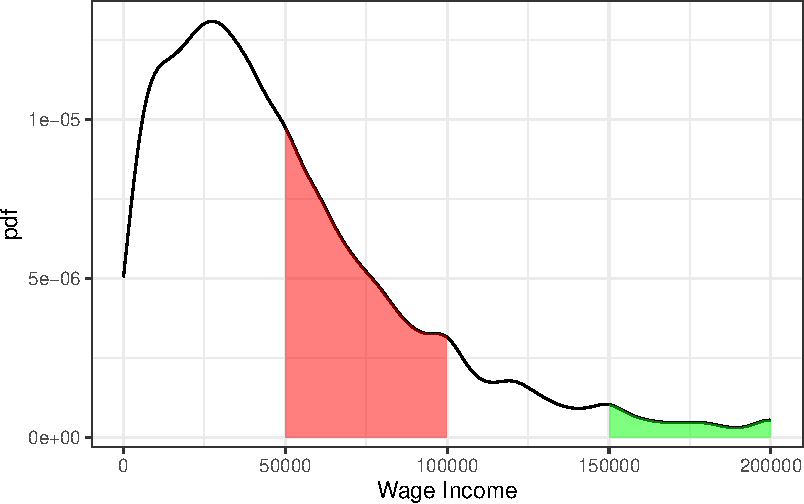
\includegraphics{03-random_variables_files/figure-pdf/unnamed-chunk-6-1.pdf}

}

\caption{pdf of U.S. wage income}

\end{figure}%

From the figure, we can see that the most common values of yearly income
are around \$25-30,000 per year. Notice that this corresponds to the
steepest part of the cdf from the previous figure. The right tail of the
distribution is also long. This means that, while incomes of \$150,000+
are not common, there are some individuals who have incomes that high.

Moreover, we can use the properties of pdfs/cdfs above to calculate some
specific probabilities. In particular, we can calculating probabilities
by calculating integrals (i.e., regions under the curve) / relating the
pdf to the cdf. First, the red region above corresponds to the
probability of a person's income being between \$50,000 and \$100,000.
This is given by \(F(100,000) - F(50000)\). We can compute this in
\texttt{R} using the \texttt{ecdf} function. In particular,

\begin{Shaded}
\begin{Highlighting}[]
\NormalTok{incwage\_cdf }\OtherTok{\textless{}{-}} \FunctionTok{ecdf}\NormalTok{(us\_data}\SpecialCharTok{$}\NormalTok{incwage)}
\FunctionTok{round}\NormalTok{(}\FunctionTok{incwage\_cdf}\NormalTok{(}\DecValTok{100000}\NormalTok{) }\SpecialCharTok{{-}} \FunctionTok{incwage\_cdf}\NormalTok{(}\DecValTok{50000}\NormalTok{),}\DecValTok{3}\NormalTok{)}
\end{Highlighting}
\end{Shaded}

\begin{verbatim}
[1] 0.27
\end{verbatim}

The green region in the figure is the probability of a person's income
being above \$150,000. Using the above properties of cdfs, we can
calculate it as \(1-F(150000)\) which is

\begin{Shaded}
\begin{Highlighting}[]
\FunctionTok{round}\NormalTok{(}\DecValTok{1}\SpecialCharTok{{-}}\FunctionTok{incwage\_cdf}\NormalTok{(}\DecValTok{150000}\NormalTok{), }\DecValTok{3}\NormalTok{)}
\end{Highlighting}
\end{Shaded}

\begin{verbatim}
[1] 0.052
\end{verbatim}

\section{Multiple Random Variables}\label{multiple-random-variables}

SW 2.3

Most often in economics, we want to consider two (or more) random
variables jointly rather than just a single random variable. For
example, mean income is interesting, but mean income as a function of
education is more interesting.

When there is more than one random variable, you can define
\textbf{joint pmfs}, \textbf{joint pdfs}, and \textbf{joint cdfs}.

Let's quickly go over these for the case where \(X\) and \(Y\) are two
discrete random variables.

\textbf{Joint pmf:} \(f_{X,Y}(x,y) := \P(X=x, Y=y)\)

\textbf{Joint cdf:} \(F_{X,Y}(x,y) := \P(X \leq x, Y \leq y)\)

\textbf{Conditional pmf:} \(f_{Y|X}(y|x) := \P(Y=y | X=x)\)

\textbf{Properties}

We use the notation that \(\mathcal{X}\) denotes the support of \(X\)
and \(\mathcal{Y}\) denotes the support of \(Y\).

\begin{enumerate}
\def\labelenumi{\arabic{enumi}.}
\item
  \(0 \leq f_{X,Y}(x,y) \leq 1\) for all \(x,y\)

  In words: the probability of \(X\) and \(Y\) taking any particular
  values can't be less than 0 or greater than 1 (because these are
  probabilities)
\item
  \(\displaystyle \sum_{x \in \mathcal{X}} \sum_{y \in \mathcal{Y}} f_{X,Y}(x,y) = 1\)

  In words: If you add up \(\P(X=x, Y=y)\) across all possible values of
  \(x\) and \(y\), they sum up to 1 (again, this is just a property of
  probabilities)
\item
  If you know the joint pmf, then you can recover the \textbf{marginal
  pmf}, that is,

  \[
   f_Y(y) = \sum_{x \in \mathcal{X}} f_{X,Y}(x,y)
   \]

  This amounts to just adding up the joint pmf across all values of
  \(x\) while holding \(y\) fixed. A main takeaway from this property is
  the following: if you know the joint pmf of two random variables, then
  it implies that you know the pmf of each random variable individuals.
  Thus, if you know the joint pmf, it implies that you know more than if
  you only knew the marginal pmfs.
\end{enumerate}

{Example: }Suppose that you roll a die, and based on this roll, you
create the following random variables.

\[
  X = \begin{cases} 0 \quad \textrm{if roll is 3 or lower} \\
  1 \quad \textrm{if roll is greater than 3} \end{cases} \qquad Y = \begin{cases} 0 \quad \textrm{if roll is odd} \\
  1 \quad \textrm{if roll is even} \end{cases}
\]

Let's consider what values \(X\) and \(Y\) take for different rolls:

\begin{longtable}[]{@{}ccc@{}}
\toprule\noalign{}
\textbf{roll} & \textbf{X} & \textbf{Y} \\
\midrule\noalign{}
\endhead
\bottomrule\noalign{}
\endlastfoot
1 & 0 & 0 \\
2 & 0 & 1 \\
3 & 0 & 0 \\
4 & 1 & 1 \\
5 & 1 & 0 \\
6 & 1 & 1 \\
\end{longtable}

Thus,

\[
\begin{aligned}
  f_{X,Y}(0, 0) = \frac{2}{6} \qquad \qquad f_{X,Y}(0,1) = \frac{1}{6} \\
  f_{X,Y}(1, 0) = \frac{1}{6} \qquad \qquad f_{X,Y}(1,1) = \frac{2}{6}
\end{aligned}
\] and you can immediately see that the first two properties hold here.
For the third property, suppose that we want to calculate \(f_Y(1)\)
(i.e., the probability that we roll an even number). The property says
that we can calculate it \[
  \begin{aligned}
  f_Y(1) &= \sum_{x=0}^1 f_{X,Y}(x,1) \\
  &= f_{X,Y}(0,1) + f_{X,Y}(1,1) = \frac{1}{6} + \frac{2}{6} = \frac{1}{2}
  \end{aligned}
\] which, as we know, is the right answer.

\(X\) and \(Y\) are said to be \textbf{independent} if
\(f_{Y|X}(y|x) = f_Y(y)\). In other words, if knowing the value of \(X\)
doesn't provide any information about the distribution \(Y\).

\bookmarksetup{startatroot}

\chapter{Expectation, Variance, and
More}\label{expectation-variance-and-more}

\[
\newcommand{\E}{\mathbb{E}}
\renewcommand{\P}{\textrm{P}}
\let\L\relax
\newcommand{\L}{\textrm{L}} %doesn't work in .qmd, place this command at start of qmd file to use it
\newcommand{\F}{\textrm{F}}
\newcommand{\var}{\textrm{var}}
\newcommand{\cov}{\textrm{cov}}
\newcommand{\corr}{\textrm{corr}}
\newcommand{\Var}{\mathrm{Var}}
\newcommand{\Cov}{\mathrm{Cov}}
\newcommand{\Corr}{\mathrm{Corr}}
\newcommand{\sd}{\mathrm{sd}}
\newcommand{\se}{\mathrm{s.e.}}
\newcommand{\T}{T}
\newcommand{\indicator}[1]{\mathbb{1}\{#1\}}
\newcommand\independent{\perp \!\!\! \perp}
\newcommand{\N}{\mathcal{N}}
\]

\section{Expected Values}\label{expected-values}

SW 2.2

The \textbf{expected value} of some random variable \(X\) is its
(population) mean and is written as \(\E[X]\). {[}I tend to write
\(\E[X]\) for the expected value, but you might also see notation like
\(\mu\) or \(\mu_X\) for the expected value.{]}

The expected value of a random variable is a \emph{feature} of its
distribution. In other words, if you know the distribution of a random
variable, then you also know its mean.

The expected value is a measure of \textbf{central tendency}
(alternative measures of central tendency are the \textbf{median} and
\textbf{mode}).

Expected values are a main concept in the course (and in
statistics/econometrics more generally). I think there are two main
reasons for this:

\begin{itemize}
\item
  Unlike a cdf, pdf, or pmf, the expected value is a single number. This
  means that it is easy to report. And, if you only knew one feature (at
  least a feature that that only involves a single number) of the
  distribution of some random variable, probably the feature that would
  be most useful to know would be the mean of the random variable.
\item
  Besides that, there are some computational reasons (we will see these
  later) that the mean can be easier to estimate than, say, the median
  of a random variable
\end{itemize}

If \(X\) is a discrete random variable, then the expected value is
defined as

\[
  \E[X] = \sum_{x \in \mathcal{X}} x f_X(x)
\]

If \(X\) is a continuous random variable, then the expected value is
defined as

\[
  \E[X] = \int_{\mathcal{X}} x f_X(x) \, dx
\] Either way, you can think of these as a weighted average of all
possible realizations of the random variable \(X\) where the weights are
given by the probability of \(X\) taking that particular value. This may
be more clear with an example\ldots{}

{Example: }Suppose that \(X\) is the outcome from a roll of a die. Then,
its expected value is given by

\[
  \begin{aligned}
  \E[X] &= \sum_{x=1}^6 x f_X(x) \\
  &= 1\left(\frac{1}{6}\right) + 2\left(\frac{1}{6}\right) + \cdots + 6\left(\frac{1}{6}\right) \\
  &= 3.5
  \end{aligned}
\]

{Side-Comment:} When we start to consider more realistic/interesting
applications, we typically won't know (or be able to easily figure out)
\(\E[X]\). Instead, we'll try to estimate it using available data. We'll
carefully distinguish between \textbf{population quantities} like
\(\E[X]\) and \textbf{sample quantities} like an estimate of \(\E[X]\)
soon.

\section{Variance}\label{variance}

SW 2.2

The next most important feature of the distribution of a random variable
is its \textbf{variance}. The variance of a random variable \(X\) is a
measure of its ``spread'', and we will denote it \(\Var(X)\) {[}You
might also sometimes see the notation \(\sigma^2\) or \(\sigma_X^2\) for
the variance.{]} The variance is defined as

\[
  \Var(X) := \E\left[ (X - \E[X])^2 \right]
\] Before we move forward, let's think about why this is a measure of
the spread of a random variable.

\begin{itemize}
\item
  \((X-\E[X])^2\) is a common way to measure the ``distance'' between
  \(X\) and \(\E[X]\). It is always positive (whether \((X - \E[X])\) is
  positive or negative) which is a good feature for a measure of
  distance to have. It is also increasing in \(|X-\E[X]|\) which also
  seems a requirement for a reasonable measure of distance.
\item
  Then, the outer expectation averages the above distance across the
  distribution of \(X\).
\end{itemize}

An alternative expression for \(\Var(X)\) that is often useful in
calculations is

\[
  \Var(X) = \E[X^2] - \E[X]^2
\]

Sometimes, we will also consider the \textbf{standard deviation} of a
random variable. The standard deviation is defined as

\[
  \textrm{sd}(X) := \sqrt{\Var(X)}
\] You might also see the notation \(\sigma\) or \(\sigma_X\) for the
standard deviation.

The standard deviation is often easier to interpret than the variance
because it has the same ``units'' as \(X\). Variance ``units'' are
squared units of \(X\).

That said, variances more often show up in formulas/derivations this
semester.

\section{Mean and Variance of Linear
Functions}\label{mean-and-variance-of-linear-functions}

SW 2.2

For this part, suppose that \(Y=a + bX\) where \(Y\) and \(X\) are
random variables while \(a\) and \(b\) are fixed constants.

\textbf{Properties of Expectations}

\begin{enumerate}
\def\labelenumi{\arabic{enumi}.}
\item
  \(\E[a] = a\) {[}In words: the expected value of a constant is just
  the constant. This holds because there is nothing random about \(a\)
  --- we just know what it is.{]}
\item
  \(\E[bX] = b\E[X]\) {[}In words: the expected value of a constant
  times a random variable is equal to the constant times the expected
  value of the random variable. We will use this property often this
  semester.{]}
\item
  \(\E[a + bX] = a + b\E[X]\) {[}In words: expected values ``pass
  through'' sums. We will use this property often this semester.{]}
\end{enumerate}

You'll also notice the similarity between the properties of summations
and expectations. This is not a coincidence --- it holds because
expectations are defined as summations (or very closely related, as
integrals).

\textbf{Properties of Variance}

\begin{enumerate}
\def\labelenumi{\arabic{enumi}.}
\item
  \(\Var(a) = 0\) {[}In words: the variance of a constant is equal to
  0.{]}
\item
  \(\Var(bX) = b^2 \Var(X)\) {[}In words: A constant can come out of the
  variance, but it needs to be squared first.{]}
\item
  \(\Var(a + bX) = \Var(bX) = b^2 \Var(X)\)
\end{enumerate}

{Example: }Later on in the semester, it will sometimes be convenient for
us to ``standardize'' some random variables. We'll talk more about the
reason to do this later, but for now, I'll just give the typical formula
for standardizing a random variable and we'll see if we can figure out
what the mean and variance of the standardized random variable are.

\[
  Y = \frac{ X - \E[X]}{\sqrt{\Var(X)}}
\] Just to be clear here, we are standardizing the random variable \(X\)
and calling its standardized version \(Y\). Let's calculate its mean

\[
  \begin{aligned}
    \E[Y] &= \E\left[ \frac{X - \E[X]}{\sqrt{\Var(X)}} \right] \\
    &= \frac{1}{\sqrt{\Var(X)}} \E\big[ X - \E[X] \big] \\
    &= \frac{1}{\sqrt{\Var(X)}} \left( \E[X] - \E\big[\E[X]\big] \right) \\
    &= \frac{1}{\sqrt{\Var(X)}} \left( \E[X] - \E[X] \right) \\
    &= 0
  \end{aligned}
\] where the first equality just comes from the definition of \(Y\), the
second equality holds because \(1/\sqrt{\Var(X)}\) is a constant and can
therefore come out of the expectation, the third equality holds because
the expectation can pass through the difference, the fourth equality
holds because \(\E[X]\) is a constant and therefore
\(\E\big[\E[X]\big] = \E[X]\), and the last equality holds because the
term in parentheses is equal to 0. Thus, the mean of \(Y\) is equal to
0. Now let's calculate the variance.

\[
  \begin{aligned}
  \Var(Y) &= \Var\left( \frac{X}{\sqrt{\Var(X)}} - \frac{\E[X]}{\sqrt{\Var(X)}} \right) \\
  &= \Var\left( \frac{X}{\sqrt{\Var(X)}}\right) \\
  &= \left( \frac{1}{\sqrt{\Var(X)}} \right)^2 \Var(X) \\
  &= \frac{\Var(X)}{\Var(X)} \\
  &= 1
  \end{aligned}
\] where the first equality holds by the definition of \(Y\), the second
equality holds because the second term is a constant and by Variance
Property 3 above, the third equality holds because
\((1/\sqrt{\Var(X)})\) is a constant and can come out of the variance
but needs to be squared, the fourth equality holds by squaring the term
on the left, and the last equality holds by cancelling the numerator and
denominator.

Therefore, we have showed that the mean of the standardized random
variable is 0 and its variance is 1. This is, in fact, the goal of
standardizing a random variable --- to transform it so that it has mean
0 and variance 1 and the particular transformation given in this example
is one that delivers a new random variable with these properties.

\section{Conditional Expectations}\label{conditional-expectations}

SW 2.3

As we discussed earlier, in economics, we often want to learn about the
relationship between several different variables. Previously, we had
discussed joint pmfs/pdfs/cdfs, and these are useful to know about.
However, they are often hard to work with in practice. For example, if
you have two random variables, visualizing their joint distribution
would involve interpreting a 3D plot which is often challenging in
practice. If you had more than two random variables, then fully
visualizing their joint distribution would not be possible. Therefore,
we will typically look at summaries of the joint distribution. Probably
the most useful one is the conditional expectation that we study in this
section; in fact, we will spend much of the semester trying to estimate
conditional expectations.

For two random variables, \(Y\) and \(X\), the \textbf{conditional
expectation} of \(Y\) given \(X=x\) is the mean value of \(Y\)
conditional on \(X\) taking the particular value \(x\). In math, this is
written

\[
  \E[Y|X=x]
\]

One useful way to think of a conditional expectation is as a
\emph{function} of \(x\). For example, suppose that \(Y\) is a person's
yearly income and \(X\) is a person's years of education. Clearly, mean
income can change for different values of education.

Conditional expectations will be a main focus of ours throughout the
semester

An extremely useful property of conditional expectations is that they
generalize from the case with two variables to the case with multiple
variables. For example, suppose that we have four random variables
\(Y\), \(X_1\), \(X_2\), and \(X_3\). It makes sense to think about \[
  \E[Y|X_1=x_1, X_2=x_2, X_3=x_3]
\] which is the expected value of \(Y\) conditional on \(X_1\) taking
the particular value \(x_1\), \(X_2\) taking the particular value
\(x_2\), and \(X_3\) taking the particular value \(x_3\). Just like
before, you can think of this as a function, in the sense that changing
any of \(x_1\), \(x_2\), and/or \(x_3\) gives a new conditional mean.

\section{Law of Iterated
Expectations}\label{law-of-iterated-expectations}

SW 2.3

Another important property of conditional expectations is called the
\textbf{law of iterated expectations}. It says that

\[
  \E[Y] = \E\big[ \E[Y|X] \big]
\] In words: The expected value of \(Y\) is equal to the expected value
(this expectation is with respect to \(X\)) of the conditional
expectation of \(Y\) given \(X\).

This may seem like a technical property, but I think the right way to
think about the law of iterated expectations is that there is an
inherent relationship between unconditional expectations and conditional
expectations. In other words, although conditional expectations can vary
arbitrarily for different values of \(X\), if you know what the
conditional expectations are, the overall expected value of \(Y\) is
fully determined.

A simple example is one where \(X\) takes only two values. Suppose we
are interested in mean birthweight (\(Y\)) for children of mother's who
either drank alcohol during their pregnancy (\(X=1\)) or who didn't
drink alcohol during their pregnancy (\(X=0\)). Suppose the following
(just to be clear, these are completely made up numbers),
\(\E[Y|X=1] = 7\), \(\E[Y|X=0]=8\) \(\P(X=1) = 0.1\) and
\(\P(X=0)=0.9\). The law of iterated expectation says that \[
  \begin{aligned}
  \E[Y] &= \E\big[ \E[Y|X] \big] \\
  &= \sum_{x \in \mathcal{X}} \E[Y|X=x] \P(X=x) \\
  &= \E[Y|X=0]\P(X=0) + \E[Y|X=1]\P(X=1) \\
  &= (8)(0.9) + (7)(0.1) \\
  &= 7.9
  \end{aligned}
\]

The law of iterated expectations still applies in more complicated cases
(e.g., \(X\) takes more than two values, \(X\) is continuous, or
\(X_1\),\(X_2\),\(X_3\)) but the intuition is still the same.

\section{Covariance}\label{covariance}

SW 2.3

The \textbf{covariance} between two random variables \(X\) and \(Y\) is
a masure of the extent to which they ``move together''. It is defined as

\[
  \Cov(X,Y) := \E[(X-\E[X])(Y-\E[Y])]
\] A natural first question to ask is: why does this measure how \(X\)
and \(Y\) move together. Notice that covariance can be positive or
negative. It will tend to be negative if big values of \(X\) (so that
\(X\) is above its mean) tend to happen at the same time as big values
of \(Y\) (so that \(Y\) is above its mean) while small values of \(X\)
(so that \(X\) is below its mean) tend to happen at the same time as
small values of \(Y\) (so that \(Y\) is below its mean).

An alternative and useful expression for covariance is \[
  \Cov(X,Y) = \E[XY] - \E[X]\E[Y]
\] Relative to the first expression, this one is probably less of a
natural definition but often more useful in mathematical problems.

One more thing to notice, if \(X\) and \(Y\) are independent, then
\(\Cov(X,Y) = 0\).

\section{Correlation}\label{correlation}

SW 2.3

It's often hard to interpret covariances directly (the ``units'' are
whatever the units of \(X\) are times the units of \(Y\)), so it is
common to scale the covariance to get the \textbf{correlation} between
two random variables:

\[
  \Corr(X,Y) := \frac{\Cov(X,Y)}{\sqrt{\Var(X)} \sqrt{\Var(Y)}}
\] The correlation has the property that it is always between \(-1\) and
\(1\).

If \(\Corr(X,Y) = 0\), then \(X\) and \(Y\) are said to be
\textbf{uncorrelated}.

\section{Properties of Expectations/Variances of Sums of
RVs}\label{properties-of-expectationsvariances-of-sums-of-rvs}

SW 2.3

Here are some more properties of expectations and variances when there
are multiple random variables. For two random variables \(X\) and \(Y\)

\begin{enumerate}
\def\labelenumi{\arabic{enumi}.}
\item
  \(\E[X+Y] = \E[X] + \E[Y]\)
\item
  \(\Var(X+Y) = \Var(X) + \Var(Y) + 2\Cov(X,Y)\)
\end{enumerate}

The first property is probably not surprising --- expectations continue
to pass through sums. The second property, particularly the covariance
term, needs more explanation. To start with, you can just plug \(X+Y\)
into the definition of variance and (with a few lines of algebra) show
that the second property is true. But, for the intuition, let me explain
with an example. Suppose that \(X\) and \(Y\) are rolls of two dice, but
\emph{somehow} these dice are positively correlated with each other ---
i.e., both rolls coming up with high numbers (and low numbers) are more
likely than with regular dice. Now, think about what the sum of two dice
rolls can be: the smallest possible sum is 2 and other values are
possible up to 12. Moreover, the smallest and largest possible sum of
the rolls (2 and 12), which are farthest away from the mean value of 7,
are relatively uncommon. You have to roll either \((1,1)\) or \((6,6)\)
to get either of these and the probability of each of those rolls is
just \(1/36\). However, when the dice are positively correlated, the
probability of both rolls being very high or very low becomes more
likely --- thus, since outcomes far away from the mean become more
likely, the variance increases.

One last comment here is that, when \(X\) and \(Y\) are independent (or
even just uncorrelated), the formula for the variance does not involve
the extra covariance term because it is equal to 0.

These properties for sums of random variables generalize to the case
with more than two random variables. For example, suppose that
\(Y_1, \ldots, Y_n\) are random variables, then

\begin{enumerate}
\def\labelenumi{\arabic{enumi}.}
\item
  \(\E\left[ \displaystyle \sum_{i=1}^n Y_i \right] = \displaystyle \sum_{i=1}^n \E[Y_i]\)
\item
  If \(Y_i\) are mutually independent, then
  \(\Var\left( \displaystyle \sum_{i=1}^n Y_i \right) = \displaystyle \sum_{i=1}^n \Var(Y_i)\)
\end{enumerate}

Notice that the last line does not involve any covariance terms, but
this is only because of the caveat that the \(Y_i\) are mutually
independent. Otherwise, there would actually be \emph{tons} of
covariance terms that would need to be accounted for.

\section{Normal Distribution}\label{normal-distribution}

SW 2.4

You probably learned about a lot of particular distributions of random
variables in your Stats class. There are a number of important
distributions:

\begin{itemize}
\item
  Normal
\item
  Binomial
\item
  t-distribution
\item
  F-distribution
\item
  Chi-squared distribution
\item
  others
\end{itemize}

SW discusses a number of these distributions, and I recommend that you
read/review those distributions. For us, the most important distribution
is the Normal distribution {[}we'll see why a few classes from now{]}.

If a random variable \(X\) follows a \textbf{normal distribution} with
mean \(\mu\) and variance \(\sigma^2\), we write

\[
  X \sim N(\mu, \sigma^2)
\] where \(\mu = \E[X]\) and \(\sigma^2 = \Var(X)\).

Importantly, if we know that \(X\) follows a normal distribution, its
entire distribution is fully characterized by its mean and variance. In
other words, if \(X\) is normally distributed, and we also know its mean
and variance, then we know everything about its distribution. {[}Notice
that this is not generally true --- if we did not know the distribution
of \(X\) but knew its mean and variance, we would know two important
features of the distribution of \(X\), but we would not know everything
about its distribution.{]}

You are probably familiar with the pdf of a normal distribution --- it
is ``bell-shaped''.

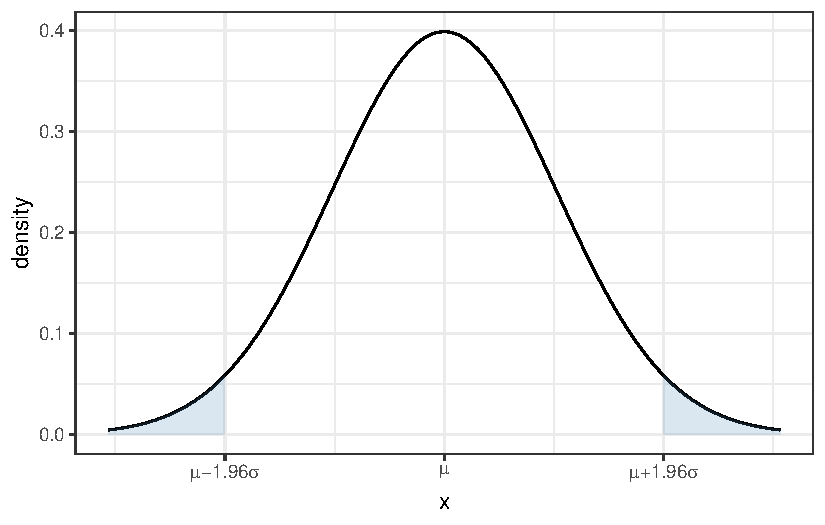
\includegraphics{04-expectations_files/figure-pdf/unnamed-chunk-2-1.pdf}

From the figure, you can see that a normal distribution is unimodal
(there is just one ``peak'') and symmetric (the pdf is the same if you
move the same distance above \(\mu\) as when you move the same distance
below \(\mu\)). This means that, for a random variable that follows a
normal distribution, its median and mode are also equal to \(\mu\).

From the plot of the pdf, we can also tell that, if you make a draw from
\(X \sim N(\mu,\sigma^2)\), the most likely values are near the mean. As
you move further away from \(\mu\), it becomes less likely (though not
impossible) for a draw of \(X\) to take that value.

Recall that we can calculate the probability that \(X\) takes on a value
in a range by calculating the area under the curve of the pdf. For each
shaded region in the figure, there is a 2.5\% chance that \(X\) falls
into that region (so the probability of \(X\) falling into either region
is 5\%). Another way to think about this is that there is a 95\%
probability that a draw of \(X\) will be in the region
\([\mu-1.96\sigma, \mu+1.96\sigma]\). Later, we we talk about hypothesis
testing, this will be an important property.

Earlier, we talked about standardizing random variables. If you know
that a random variable follows a normal distribution, it is very common
to standardize it. In particular notice that, if you create the
standardized random variable

\[
  Z := \frac{X - \mu}{\sigma} \quad \textrm{then} \quad Z \sim N(0,1)
\] If you think back to your probability and statistics class, you may
have done things like calculating a p-value by looking at a ``Z-table''
in the back of a textbook (I'm actually not sure if this is still
commonly done because it is often easier to just do this on a computer,
but, back in ``my day'' this was a very common exercise in statistics
classes). Standardizing allows you to look at just one table for any
normally distributed random variable that you could encounter rather
than requiring you to have different Z table for each value of \(\mu\)
and \(\sigma^2\).

\section{Coding}\label{coding}

To conclude this section, we'll use R to compute the features of the
joint distribution of income and education that we have discussed above.

\begin{Shaded}
\begin{Highlighting}[]
\CommentTok{\# create vectors of income and educ}
\NormalTok{income }\OtherTok{\textless{}{-}}\NormalTok{ us\_data}\SpecialCharTok{$}\NormalTok{incwage}
\NormalTok{educ }\OtherTok{\textless{}{-}}\NormalTok{ us\_data}\SpecialCharTok{$}\NormalTok{educ}

\CommentTok{\# mean of income}
\FunctionTok{mean}\NormalTok{(income)}
\end{Highlighting}
\end{Shaded}

\begin{verbatim}
[1] 58605.75
\end{verbatim}

\begin{Shaded}
\begin{Highlighting}[]
\CommentTok{\# mean of education}
\FunctionTok{mean}\NormalTok{(educ)}
\end{Highlighting}
\end{Shaded}

\begin{verbatim}
[1] 13.96299
\end{verbatim}

\begin{Shaded}
\begin{Highlighting}[]
\CommentTok{\# variance}
\FunctionTok{var}\NormalTok{(income)}
\end{Highlighting}
\end{Shaded}

\begin{verbatim}
[1] 4776264026
\end{verbatim}

\begin{Shaded}
\begin{Highlighting}[]
\FunctionTok{var}\NormalTok{(educ)}
\end{Highlighting}
\end{Shaded}

\begin{verbatim}
[1] 8.345015
\end{verbatim}

\begin{Shaded}
\begin{Highlighting}[]
\CommentTok{\# standard deviation}
\FunctionTok{sd}\NormalTok{(income)}
\end{Highlighting}
\end{Shaded}

\begin{verbatim}
[1] 69110.52
\end{verbatim}

\begin{Shaded}
\begin{Highlighting}[]
\FunctionTok{sd}\NormalTok{(educ)}
\end{Highlighting}
\end{Shaded}

\begin{verbatim}
[1] 2.888774
\end{verbatim}

\begin{Shaded}
\begin{Highlighting}[]
\CommentTok{\# covariance}
\FunctionTok{cov}\NormalTok{(income,educ)}
\end{Highlighting}
\end{Shaded}

\begin{verbatim}
[1] 63766.72
\end{verbatim}

\begin{Shaded}
\begin{Highlighting}[]
\CommentTok{\# correlation}
\FunctionTok{cor}\NormalTok{(income, educ)}
\end{Highlighting}
\end{Shaded}

\begin{verbatim}
[1] 0.3194011
\end{verbatim}

\section{Lab 2: Basic Plots}\label{lab-2-basic-plots}

Related Reading: IDS 9.4 (if you are interested, you can read IDS
Chapters 6-10 for much more information about plotting in \texttt{R})

In this lab, I'll introduce you to some basic plotting. Probably the
most common type of plot that I use is a line plot. We'll go for trying
to make a line plot of average income as a function of education.

To start with, I'll introduce you to R's \texttt{ggplot2} package. This
is one of the most famous plot-producing packages (not just in R, but
for any programming language). The syntax may be somewhat challenging to
learn, but I think it is worth it to exert some effort here.

{Side Comment:} Base \texttt{R} has several plotting functions (e.g.,
\texttt{plot}). Check IDS 2.15 for an introduction to these functions.
These are generally easier to learn but less beautiful than plots coming
from \texttt{ggplot2}.

\begin{Shaded}
\begin{Highlighting}[]
\CommentTok{\# load ggplot2 package}
\CommentTok{\# (if you haven\textquotesingle{}t installed it, you would need to do that first)}
\FunctionTok{library}\NormalTok{(ggplot2)}

\CommentTok{\# load dplyr package for "wrangling" data}
\FunctionTok{library}\NormalTok{(dplyr)}
\end{Highlighting}
\end{Shaded}

\begin{Shaded}
\begin{Highlighting}[]
\CommentTok{\# arrange data}
\NormalTok{plot\_data }\OtherTok{\textless{}{-}}\NormalTok{ us\_data }\SpecialCharTok{\%\textgreater{}\%}
    \FunctionTok{group\_by}\NormalTok{(educ) }\SpecialCharTok{\%\textgreater{}\%}
    \FunctionTok{summarize}\NormalTok{(}\AttributeTok{income=}\FunctionTok{mean}\NormalTok{(incwage))}

\CommentTok{\# make the plot}
\FunctionTok{ggplot}\NormalTok{(}\AttributeTok{data=}\NormalTok{plot\_data,}
       \AttributeTok{mapping=}\FunctionTok{aes}\NormalTok{(}\AttributeTok{x=}\NormalTok{educ,}\AttributeTok{y=}\NormalTok{income)) }\SpecialCharTok{+}
    \FunctionTok{geom\_line}\NormalTok{() }\SpecialCharTok{+}
    \FunctionTok{geom\_point}\NormalTok{(}\AttributeTok{size=}\DecValTok{3}\NormalTok{) }\SpecialCharTok{+}
    \FunctionTok{theme\_bw}\NormalTok{()}
\end{Highlighting}
\end{Shaded}

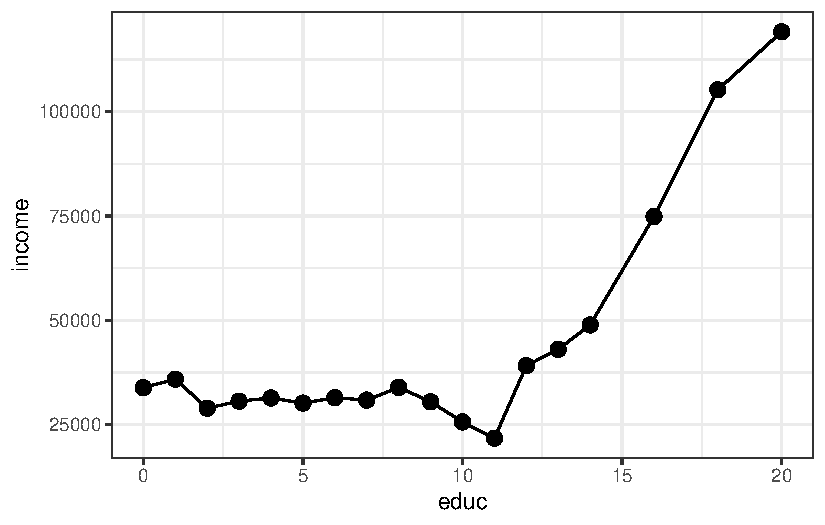
\includegraphics{04-expectations_files/figure-pdf/unnamed-chunk-5-1.pdf}

Let me explain what's going on here piece-by-piece. Let's start with
this code

\begin{Shaded}
\begin{Highlighting}[]
\CommentTok{\# arrange data}
\NormalTok{plot\_data }\OtherTok{\textless{}{-}}\NormalTok{ us\_data }\SpecialCharTok{\%\textgreater{}\%}
    \FunctionTok{group\_by}\NormalTok{(educ) }\SpecialCharTok{\%\textgreater{}\%}
    \FunctionTok{summarize}\NormalTok{(}\AttributeTok{income=}\FunctionTok{mean}\NormalTok{(incwage))}
\end{Highlighting}
\end{Shaded}

At a high-level, making plots often involves two steps --- first
arranging the data in the ``appropriate'' way (that's this step) and
then actually making the plot.

This is ``tidyverse-style'' code too --- in my view, it is a little
awkward, but it is also common so I think it is worth explaining here a
bit.

First, the \textbf{pipe operator}, \texttt{\%\textgreater{}\%} takes the
thing on the left of it and applies the function to the right of it. So,
the line \texttt{us\_data\ \%\textgreater{}\%\ group\_by(educ)} takes
\texttt{us\_data} and applies the function \texttt{group\_by} to it, and
what we group by is \texttt{educ}. That creates a new data frame (you
could just run that code and see what you get). The next line takes that
new data frame and applies the function \texttt{summarize} to it. In
this case, \texttt{summarize} creates a new variable called
\texttt{income} that is the mean of the column \texttt{incwage} and it
is the mean by \texttt{educ} (since we grouped by education in the
previous step).

Take a second and look through what has actually been created here.
\texttt{plot\_data} is a new data frame, but it only has 18 observations
--- corresponding to each distinct value of education in the data. It
also has two columns, the first one is \texttt{educ} which is the years
of education, and the second one is \texttt{income} which is the average
income among individuals that have that amount of education.

An alternative way of writing the exact same code (that seems more
natural to me) is

\begin{Shaded}
\begin{Highlighting}[]
\CommentTok{\# arrange data}
\NormalTok{grouped\_data }\OtherTok{\textless{}{-}} \FunctionTok{group\_by}\NormalTok{(us\_data, educ)}
\NormalTok{plot\_data }\OtherTok{\textless{}{-}} \FunctionTok{summarize}\NormalTok{(grouped\_data, }\AttributeTok{income=}\FunctionTok{mean}\NormalTok{(incwage))}
\end{Highlighting}
\end{Shaded}

If you're familiar with other programming languages, the second version
of the code probably seems more familiar. Either way is fine with me ---
tidyverse-style seems to be trendy in R programming these days, but (for
me) I think the second version is a little easier to understand. You can
find long ``debates'' about these two styles of writing code if you
happen to be interested\ldots{}

Before moving on, let me mention a few other \texttt{dplyr} functions
that you might find useful

\begin{itemize}
\item
  \texttt{filter} --- this is tidy version of \texttt{subset}
\item
  \texttt{select} --- selects particular columns of interest from your
  data
\item
  \texttt{mutate} --- creates a new variable from existing columns in
  your data
\item
  \texttt{arrange} --- useful for sorting your data
\end{itemize}

Next, let's consider the second part of the code.

\begin{Shaded}
\begin{Highlighting}[]
\CommentTok{\# make the plot}
\FunctionTok{ggplot}\NormalTok{(}\AttributeTok{data=}\NormalTok{plot\_data,}
       \AttributeTok{mapping=}\FunctionTok{aes}\NormalTok{(}\AttributeTok{x=}\NormalTok{educ,}\AttributeTok{y=}\NormalTok{income)) }\SpecialCharTok{+}
    \FunctionTok{geom\_line}\NormalTok{() }\SpecialCharTok{+}
    \FunctionTok{geom\_point}\NormalTok{(}\AttributeTok{size=}\DecValTok{3}\NormalTok{) }\SpecialCharTok{+}
    \FunctionTok{theme\_bw}\NormalTok{()}
\end{Highlighting}
\end{Shaded}

The main function here is \texttt{ggplot}. It takes in two main
arguments: \texttt{data} and \texttt{mapping}. Notice that we set
\texttt{data} to be equal to \texttt{plot\_data} which is the data frame
that we just created. The \texttt{mapping} is set equal to
\texttt{aes(x=educ,y=income)}. \texttt{aes} stands for ``aesthetic'',
and here you are just telling \texttt{ggplot} the names of the columns
in the data frame that should be on the x-axis (here: \texttt{educ}) and
on the y-axis (here: \texttt{income}) in the plot. Also, notice the
\texttt{+} at the end of the line; you can interpret this as saying
``keep going'' to the next line before executing.

If we just stopped there, we actually wouldn't plot anything. We still
need to tell \texttt{ggplot} what kind of plot we want to make. That's
where the line \texttt{geom\_line} comes in. It tells \texttt{ggplot}
that we want to plot a line. Try running the code with just those two
lines --- you will see that you will get a similar (but not exactly the
same) plot.

\texttt{geom\_point} adds the dots in the figure. \texttt{size=3}
controls the size of the points. I didn't add this argument originally,
but the dots were hard to see so I made them bigger.

\texttt{theme\_bw} changes the color scheme of the plot. It stands for
``theme black white''.

There is a ton of flexibility with \texttt{ggplot} --- way more than I
could list here. But let me give you some extras that I tend to use
quite frequently.

\begin{itemize}
\item
  In \texttt{geom\_line} and \texttt{geom\_point}, you can add the extra
  argument \texttt{color}; for example, you could try
  \texttt{geom\_line(color="blue")} and it would change the color of the
  line to blue.
\item
  In \texttt{geom\_line}, you can change the ``type'' of the line by
  using the argument \texttt{linetype}; for example,
  \texttt{geom\_line(linetype="dashed")} would change the line from
  being solid to being dashed.
\item
  In \texttt{geom\_line}, the argument \texttt{size} controls the
  thickness of the line.
\item
  The functions \texttt{ylab} and \texttt{xlab} control the labels on
  the y-axis and x-axis
\item
  The functions \texttt{ylim} and \texttt{xlim} control the ``limits''
  of the y-axis and x-axis. Here's how you can use these:

\begin{Shaded}
\begin{Highlighting}[]
\CommentTok{\# make the plot}
\FunctionTok{ggplot}\NormalTok{(}\AttributeTok{data=}\NormalTok{plot\_data,}
     \AttributeTok{mapping=}\FunctionTok{aes}\NormalTok{(}\AttributeTok{x=}\NormalTok{educ,}\AttributeTok{y=}\NormalTok{income)) }\SpecialCharTok{+}
  \FunctionTok{geom\_line}\NormalTok{() }\SpecialCharTok{+}
  \FunctionTok{geom\_point}\NormalTok{(}\AttributeTok{size=}\DecValTok{3}\NormalTok{) }\SpecialCharTok{+}
  \FunctionTok{theme\_bw}\NormalTok{() }\SpecialCharTok{+}
\NormalTok{  ylim}\OtherTok{=}\FunctionTok{c}\NormalTok{(}\DecValTok{0}\NormalTok{,}\DecValTok{150000}\NormalTok{) }\SpecialCharTok{+}
  \FunctionTok{ylab}\NormalTok{(}\StringTok{"Income"}\NormalTok{) }\SpecialCharTok{+}
  \FunctionTok{xlab}\NormalTok{(}\StringTok{"Education"}\NormalTok{)}
\end{Highlighting}
\end{Shaded}

  which will adjust the y-axis and change the labels on each axis.
\end{itemize}

Besides the line plot (using \texttt{geom\_line}) and the scatter plot
(using \texttt{geom\_point}), probably two other types of plots that I
make the most are

\begin{itemize}
\item
  Histogram (using \texttt{geom\_histogram}) --- this is how I made the
  plot of the pmf of education earlier in this chapter
\item
  Adding a straight line to a plot (using \texttt{geom\_abline} which
  takes in \texttt{slope} and \texttt{intercept} arguments) --- we
  haven't used this yet, but we will win once we start talking about
  regressions
\item
  If you're interested, here is a to a large number of different types
  of plots that are available using \texttt{ggplot}:
  \url{http://r-statistics.co/Top50-Ggplot2-Visualizations-MasterList-R-Code.html}
\end{itemize}

\section{In Case You're Interested: Chebyshev's
Inequality}\label{in-case-youre-interested-chebyshevs-inequality}

As discussed above, the standard deviation is a measure of the spread of
a random variable that is in units that are easy to understand. But what
exactly does it tell us about the spread of a random variable? One way
to think about the spread of a random variable is to think about the
probability that a random variable will take a value within a certain
range. For example, when we talked about the normal distribution, we
said that there is a 95\% chance that a draw of a normally distributed
random variable will be within 1.96 standard deviations of the mean.
This is a very specific statement about the spread of a random variable.

But the claim that there is a 95\% chance that a random variable will be
within 1.96 standard deviations of its mean only holds for normally
distributed random variables. \textbf{Chebyshev's Inequality} provides a
way to relate the standard deviation of a random variable to the
probability that it will take a value within a certain range, for any
random variable (i.e., the variable can follow essentially any
distribution). Chebyshev's Inequality says that, for any random variable
\(X\) and any \(k > 0\), \begin{align*}
  \P\Big(\big|X - \E[X]\big| \geq k \cdot \sd(X) \Big) \leq \frac{1}{k^2}
\end{align*} This holds for any \(k\), so let's pick an interesting
value and be a bit more specific. Suppose that \(k=2\). Then,
Chebyshev's Inequality says that the probability that a random variable
will be more than 2 standard deviations away from its mean is less than
or equal to \(1/4\). Let's compare this to the case where we know that
\(X\) follows a normal distribution. In that case, there's a 95\% chance
that \(X\) will be within (essentially) 2 standard deviations of its
mean; if we don't know that \(X\) follows a normal distribution, then we
can't make as strong a statement, but we can say that at least 75\% of
the time, \(X\) will be within 2 standard deviations of its mean. You
can try other values of \(k\) too.

\section{Coding Questions}\label{coding-questions}

\begin{enumerate}
\def\labelenumi{\arabic{enumi}.}
\item
  Run the following code to create the data that we will use in the
  problem

\begin{Shaded}
\begin{Highlighting}[]
\FunctionTok{set.seed}\NormalTok{(}\DecValTok{1234}\NormalTok{) }\CommentTok{\# setting the seed means that we will get the same results}
\NormalTok{x }\OtherTok{\textless{}{-}} \FunctionTok{rexp}\NormalTok{(}\DecValTok{100}\NormalTok{) }\CommentTok{\# make 100 draws from an exponential distribution}
\end{Highlighting}
\end{Shaded}

  Use the \texttt{ggplot2} package to plot a histogram of \texttt{x}.
\item
  For this question, we'll use the data \texttt{fertilizer\_2000}. A
  scatter plot is a useful way to visualize 2-dimensional data. Use the
  \texttt{ggplot2} package to make a scatter plot with crop yield
  (\texttt{avyield}) on the y-axis and fertilizer (\texttt{avfert}) on
  the x-axis. Label the y-axis ``Crop Yield'' and the x-axis
  ``Fertilizer''. Do you notice any pattern from the scatter plot?
\end{enumerate}

\section{Extra Questions}\label{extra-questions}

\begin{enumerate}
\def\labelenumi{\arabic{enumi}.}
\item
  Suppose that \(\E[X] = 10\) and \(\var(X) = 2\). Also, suppose that
  \(Y=5 + 9 X\).

  \begin{enumerate}
  \def\labelenumii{\alph{enumii})}
  \item
    What is \(\E[Y]\)?
  \item
    What is \(\var(Y)\)?
  \end{enumerate}
\item
  Use the definition of variance to show that \(\Var(bX) = b^2 \Var(X)\)
  (where \(b\) is a constant and \(X\) is some random variable).
\item
  Suppose you are interested in average height of students at UGA. Let
  \(Y\) denote a student's height; also let \(X\) denote a binary
  variable that is equal to 1 if a student is female. Suppose that you
  know that \(\E[Y|X=1] = 5' \,4''\) and that \(\E[Y|X=0] = 5' \,9''\)
  (and that \(\P(X=1) = 0.5\)).

  \begin{enumerate}
  \def\labelenumii{\alph{enumii})}
  \item
    What is \(\E[Y]\)?
  \item
    Explain how the answer to part (a) is related to the Law of Iterated
    Expectations.
  \end{enumerate}
\item
  Consider a random variable \(X\) with support
  \(\mathcal{X} = \{2,7,13,21\}\). Suppose that it has the following
  pmf:

  \[
      \begin{aligned}
       f_X(2) &= 0.5 \\
       f_X(7) &= 0.25 \\
       f_X(13) &= 0.15 \\
       f_X(21) &= ??
     \end{aligned}
   \]

  \begin{enumerate}
  \def\labelenumii{\alph{enumii})}
  \item
    What is \(f_X(21)\)? How do you know?
  \item
    What is the expected value of \(X\)? {[}Show your calculation.{]}
  \item
    What is the variance of \(X\)? {[}Show your calculation.{]}
  \item
    Calculate \(F_X(x)\) for \(x=1\), \(x=7\), \(x=8\), and \(x=25\).
  \end{enumerate}
\end{enumerate}

\part{Properties of Estimators}

\bookmarksetup{startatroot}

\chapter{Finite Sample Properties}\label{finite-sample-properties}

\[
\newcommand{\E}{\mathbb{E}}
\renewcommand{\P}{\textrm{P}}
\let\L\relax
\newcommand{\L}{\textrm{L}} %doesn't work in .qmd, place this command at start of qmd file to use it
\newcommand{\F}{\textrm{F}}
\newcommand{\var}{\textrm{var}}
\newcommand{\cov}{\textrm{cov}}
\newcommand{\corr}{\textrm{corr}}
\newcommand{\Var}{\mathrm{Var}}
\newcommand{\Cov}{\mathrm{Cov}}
\newcommand{\Corr}{\mathrm{Corr}}
\newcommand{\sd}{\mathrm{sd}}
\newcommand{\se}{\mathrm{s.e.}}
\newcommand{\T}{T}
\newcommand{\indicator}[1]{\mathbb{1}\{#1\}}
\newcommand\independent{\perp \!\!\! \perp}
\newcommand{\N}{\mathcal{N}}
\]

So far, we have been talking about \textbf{population quantities} such
as \(f_{Y|X}\) (conditional pdf/pmf), \(\E[Y]\) (expected value of
\(Y\)), or \(\E[Y|X]\) (expected value of \(Y\) given \(X\)).

In practice, most often we do not know what these population quantities
are equal to (with the exception of some trivial cases like flipping a
coin or rolling a die).

A fundamental challenge is that it is uncommon that we observe the
entire population.

Instead, we will take the approach that we have access to a
\textbf{sample} of data from the original population. We'll use the
sample to try to \textbf{estimate} whatever population quantities we are
interested in as well as develop the tools to \textbf{conduct
inference}, paying particular interest to questions like: how precisely
can we estimate particular population quantities of interest?

The topics considered in this section fall broadly under the topic of
\textbf{statistics} (a reasonable definition of statistics is that it is
the set of tools to learn about population quantities using data). Some
of this material may be familiar from courses that you have taken
before, but this section provides a fairly advanced discussion of these
issues with a particular eye towards (i) inference issues that are
important econometrics and (ii) prediction problems. Many of the tools
that we cover in this section will be used throughout the rest of the
course.

\section{Simple Random Sample}\label{simple-random-sample}

SW 2.5

Let's start by talking about how the data that we have access to is
collected. There are several possibilities here, but let us start with
the most straightforward case (which is also a very common case) called
a \textbf{simple random sample}.

In math: \(\{Y_i\}_{i=1}^n\) is called a simple random sample if
\(Y_1, Y_2, \ldots, Y_n\) are independent random variables with a common
probability distribution \(f_Y\). The two key conditions here are (i)
independence and (ii) from a common distribution. For this reason, you
may sometimes see a random sample called an iid sample which stands for
independent and identically distributed.

In words: We have access to \(n\) observations that are drawn at random
from some underlying population and each observation is equally likely
to be drawn.

\section{\texorpdfstring{Estimating
\(\E[Y]\)}{Estimating \textbackslash E{[}Y{]}}}\label{estimating-ey}

SW 2.5, 3.1

Let's start with trying to estimate \(\E[Y]\) as this is probably the
simplest, non-trivial thing that we can estimate.

A natural way to estimate population quantities is with their sample
analogue. This is called the \textbf{analogy principle}. This is perhaps
technical jargon, but it is the way you would immediately think to
estimate \(\E[Y]\):

\[
  \hat{\E}[Y] = \frac{1}{n} \sum_{i=1}^n Y_i = \bar{Y}
\] In this course, we will typically put a ``hat'' on estimated
quantities. The expression \(\displaystyle \frac{1}{n}\sum_{i=1}^n Y_i\)
is just the average value of \(Y\) in our sample. Since we will
calculate a ton of averages like this one over the course of the rest of
the semester, it's also convenient to give it a shorthand notation,
which is what \(\bar{Y}\) means --- it is just the sample average of
\(Y\).

One thing that is important to be clear about at this point is that, in
general, \(\E[Y] \neq \bar{Y}\). \(\E[Y]\) is a population quantity
while \(\bar{Y}\) is a sample quantity. We will hope (and provide some
related conditions/discussions below) that \(\bar{Y}\) would be close to
\(\E[Y]\), but, in general, they will not be exactly the same.

\section{\texorpdfstring{Mean of
\(\bar{Y}\)}{Mean of \textbackslash bar\{Y\}}}\label{mean-of-bary}

SW 2.5, 3.1

Another important thing to notice about \(\bar{Y}\) is that it is a
random variable (as it is the average of random variables). This is in
sharp contrast to \(\E[Y]\) which is non-random.

One related thought experiment is the following: if we could repeatedly
collect new samples of size \(n\) from the same population and each time
were able to estimate \(\bar{Y}\), these estimates would be different
from each other.

In fact, this means that \(\bar{Y}\) has a distribution. The
distribution of a statistic, like \(\bar{Y}\), is called its
\textbf{sampling distribution}. We'd like to know about the features of
the sampling distribution. Let's start with its mean. That is, let's
calculate

\[
  \begin{aligned}
    \E[\bar{Y}] &= \E\left[ \frac{1}{n} \sum_{i=1}^n Y_i \right] \\
    &= \frac{1}{n} \E\left[ \sum_{i=1}^n Y_i \right] \\
    &= \frac{1}{n} \sum_{i=1}^n \E[Y_i] \\
    &= \frac{1}{n} \sum_{i=1}^n \E[Y] \\
    &= \frac{1}{n} n \E[Y] \\
    &= \E[Y]
  \end{aligned}
\] Let's think carefully about each step here --- the arguments rely
heavily on the properties of expectations and summations that we have
learned earlier. The first equality holds from the definition of
\(\bar{Y}\). The second equality holds because \(1/n\) is a constant and
can therefore come out of the expectation. The third equality holds
because the expectation can pass through the sum. The fourth equality
holds because \(Y_i\) are all from the same distribution which implies
that they all of the same mean and that it is equal to \(\E[Y]\). The
fifth equality holds because \(\E[Y]\) is a constant and we add it up
\(n\) times. And the last equality just cancels the \(n\) in the
numerator with the \(n\) in the denominator.

Before moving on, let me make an additional comment:

\begin{itemize}
\tightlist
\item
  The fourth equality might be a little confusing. Certainly it is not
  saying that all the \(Y_i\)'s are equal to each other. Rather, they
  come from the same distribution. For example, if you roll a die \(n\)
  times, you get different outcomes on different rolls, but they are all
  from the same distribution so that the population expectation of each
  roll is always 3.5, but you get different realizations on different
  particular rolls. Another example is if \(Y\) is a person's income.
  Again, we are not saying that everyone has the same income, but just
  that we are thinking of income as being a draw from some distribution
  --- sometimes you get a draw of a person with a very high income;
  other times you get a draw of a person with a low income, but
  \(\E[Y]\) is a feature of the underlying distribution itself where
  these draws come from.
\end{itemize}

How should interpret the above result? It says that,
\(\E[\bar{Y}] = \E[Y]\). This doesn't mean that \(\bar{Y}\) itself is
equal to \(\E[Y]\). Rather, it means that, if we could repeatedly obtain
(a huge number of times) new samples of size \(n\) and compute
\(\bar{Y}\) each time, the average of \(\bar{Y}\) across repeated
samples would be equal to \(\E[Y]\).

\section{\texorpdfstring{Variance of
\(\bar{Y}\)}{Variance of \textbackslash bar\{Y\}}}\label{variance-of-bary}

SW 2.5, 3.1

Next, let's calculate the variance of \(\bar{Y}\). As before, we are
continuing with the thought experiment of being able to repeatedly draw
new samples of size \(n\), and, therefore, we call this variance the
\textbf{sampling variance}.

\[
  \begin{aligned}
    \Var(\bar{Y}) &= \Var\left(\frac{1}{n} \sum_{i=1}^n Y_i\right) \\
    &= \frac{1}{n^2} \Var\left(\sum_{i=1}^n Y_i\right) \\
    &= \frac{1}{n^2} \left( \sum_{i=1}^n \Var(Y_i) + \textrm{lots of covariance terms} \right) \\
    &= \frac{1}{n^2} \left( \sum_{i=1}^n \Var(Y_i) \right) \\
    &= \frac{1}{n^2} \sum_{i=1}^n \Var(Y) \\
    &= \frac{1}{n^2} n \Var(Y) \\
    &= \frac{\Var(Y)}{n}
  \end{aligned}
\] Let's go carefully through each step --- these arguments rely heavily
on the properties of variance that we talked about earlier. The first
equality holds by the definition of \(\bar{Y}\). The second equality
holds because \(1/n\) is a constant and can come out of the variance
after squaring it. The third equality holds because the variance of the
sum of random variables is equal to the sum of the variances plus all
the covariances between the random variables. In the fourth equality,
all of the covariance terms go away --- this holds because of random
sampling which implies that the \(Y_i\) are all independent which
implies that their covariances are equal to 0. The fifth equality holds
because all \(Y_i\) are identically distributed so their variances are
all the same and equal to \(\Var(Y)\). The sixth equality holds by
adding up \(\Var(Y)\) \(n\) times. The last equality holds by canceling
the \(n\) in the numerator with one of the \(n\)'s in the denominator.

Interestingly, the variance of \(\bar{Y}\) depends not just on
\(\Var(Y)\) but also on \(n\) --- the number of observations in the
sample. Notice that \(n\) is in the denominator, so the variance of
\(\bar{Y}\) will be lower for large values of \(n\). Here is an example
that may be helpful for understanding this. Suppose that you are rolling
a die. If \(n=1\), then clearly, the variance of \(\bar{Y}\) is just
equal to the variance of \(Y\) --- sometimes you roll extreme values
like \(1\) or \(6\). Now, when you increase \(n\), say, to 10, then
these extreme values of \(\bar{Y}\) are substantially less common. For
\(\bar{Y}\) to be equal to \(6\) in this case, you'd need to roll 10
\(6\)'s in a row. This illustrates that the sampling variance of
\(\bar{Y}\) is decreasing in \(n\). If this is not perfectly clear, we
will look at some data soon, and I think that should confirm to you that
the variance of \(\bar{Y}\) is decreasing in the sample size.

\section{Properties of Estimators}\label{properties-of-estimators-1}

SW 2.5, 3.1

Suppose we are interested in some population parameter \(\theta\) ---
we'll write this pretty generically now, but it could be \(\E[Y]\) or
\(\E[Y|X]\) or really any other population quantity that you'd like to
estimate.

Also, suppose that we have access to a random sample of size \(n\) and
we have some estimate of \(\theta\) that we'll call \(\hat{\theta}\).

As before, we are going to consider the repeated sampling thought
experiment where we imagine that we could repeatedly obtain new samples
of size \(n\) and with each new sample calculate a new \(\hat{\theta}\).
Under this thought experiment, \(\hat{\theta}\) would have a sampling
distribution. One possibility for what it could look like is the
following

\includegraphics{05-finite_sample_properties_files/figure-pdf/unnamed-chunk-1-1.pdf}

In this case, values of \(\hat{\theta}\) are more common around 3 and 4,
but it is not highly unusual to get a value of \(\hat{\theta}\) that is
around 1 or 2 or 5 or 6 either.

The first property of an estimator that we will take about is called
\textbf{unbiasedness}. An estimator \(\hat{\theta}\) is said to be
unbiased if \(\E[\hat{\theta}] = \theta\). Alternatively, we can define
the \textbf{bias} of an estimator as

\[
  \textrm{Bias}(\hat{\theta}) = \E[\hat{\theta}] - \theta
\] For example, if \(\textrm{Bias}(\hat{\theta}) > 0\), it means that,
on average (in the repeated sampling thought experiment), our estimates
of \(\theta\) would be greater than the actual value of \(\theta\).

In general, unbiasedness is a good property for an estimator to have.
That being said, we can come up with examples of not-very-good unbiased
estimators and good biased estimators, but all-else-equal, it is better
for an estimator to be unbiased.

The next property of estimators that we will talk about is their
\textbf{sampling variance}. This is just \(\Var(\hat{\theta})\). In
general, we would like estimators with low (or 0) bias and low sampling
variance. Let me give an example

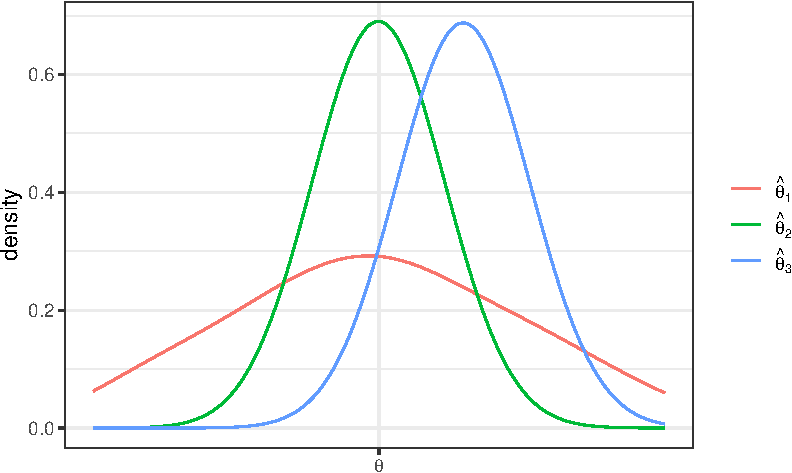
\includegraphics{05-finite_sample_properties_files/figure-pdf/unnamed-chunk-2-1.pdf}

This is a helpful figure for thinking about the properties of
estimators. In this case, \(\hat{\theta}_1\) and \(\hat{\theta}_2\) are
both unbiased (because their means are \(\theta\)) while
\(\hat{\theta}_3\) is biased --- it's mean is greater than \(\theta\).
On the other hand the sampling variance of \(\hat{\theta}_2\) and
\(\hat{\theta}_3\) are about the same and both substantially smaller
than for \(\hat{\theta}_1\). Clearly, \(\hat{\theta}_2\) is the best
estimator of \(\theta\) out of the three. But which is the second best?
It is not clear. \(\hat{\theta}_3\) systematically over-estimates
\(\theta\), but since the variance is relatively small, the misses are
systematic but tend to be relatively small. On the other hand,
\(\hat{\theta}_1\) is, on average, equal to \(\theta\), but sometimes
the estimate of \(\theta\) could be quite poor due to the large sampling
variance.

\section{Relative Efficiency}\label{relative-efficiency}

SW 3.1

If \(\hat{\theta}_1\) and \(\hat{\theta}_2\) are two unbiased estimators
of \(\theta\), then \(\hat{\theta}_1\) is \textbf{more efficient} than
\(\hat{\theta}_2\) if \(\Var(\hat{\theta}_1) < \Var(\hat{\theta}_2)\).

Relative efficiency gives us a way to rank unbiased estimators.

\section{Mean Squared Error}\label{mean-squared-error}

More generally, two estimators can be compared by their \textbf{mean
squared error} which is defined as

\[
  \textrm{MSE}(\hat{\theta}) := \E\left[ (\hat{\theta} - \theta)^2\right]
\]

The mean squared error of \(\hat{\theta}\) is the average ``distance''
between \(\hat{\theta}\) and \(\theta\) in the thought experiment of
having repeated samples of size \(n\).

Another equivalent expression for the mean squared error is

\[
  \textrm{MSE}(\hat{\theta}) = \textrm{Bias}(\hat{\theta})^2 + \Var(\hat{\theta})
\] In other words, if we can figure out the bias and variance of
\(\hat{\theta}\), then we can recover mean squared error.

{Side-Comment:} I think it is worth quickly explaining where the second
expression for \(\textrm{MSE}(\hat{\theta})\) comes from. Starting from
the definition of \(\textrm{MSE}(\hat{\theta})\),

\[
  \begin{aligned}
    \textrm{MSE}(\hat{\theta}) &= \E\left[ (\hat{\theta} - \theta)^2\right] \\
    &= \E\left[ \left( (\hat{\theta} - \E[\hat{\theta}]) + (\E[\hat{\theta}] - \theta)\right)^2 \right] \\
    &= \E\left[ (\hat{\theta} - \E[\hat{\theta}])^2 \right] + \E\left[ (\E[\hat{\theta}] - \theta)^2\right] + 2 \E\left[ (\hat{\theta} - \E[\hat{\theta}])(\E[\hat{\theta}] - \theta) \right] \\
    &= \Var(\hat{\theta}) + \textrm{Bias}(\hat{\theta})^2 
  \end{aligned}
\] where the first equality is just the definition of
\(\textrm{MSE}(\hat{\theta})\), the second equality adds and subtracts
\(\E[\hat{\theta}]\), the third equality squares everything in
parentheses from the previous line and pushes the expectation through
the sum. For the last equality, the first term in the previous line
corresponds to the definition of \(\Var(\hat{\theta})\); for the second
term, recall that
\(\textrm{Bias}(\hat{\theta}) = \E[\hat{\theta}-\theta]\) (and this is
non-random so the outside expectation just goes away); the last term is
equal to 0 which just holds by the properties of expectations after
noticing that \((\E[\hat{\theta}] - \theta)\) is non-random and can
therefore come out of the expectation.

Generally, we would like to choose estimators that have low mean squared
error (this essentially means that they have low bias and variance).
Moreover, mean squared error gives us a way to compare estimators that
are potentially biased. {[}Also, notice that for unbiased estimators,
comparing mean squared errors of different estimators just compares
their variance (because the bias term is equal to 0), so this is a
\emph{generalization} of relative efficiency from the previous
section.{]}

{Example: }Let's compare three estimators of \(\E[Y]\) based on their
mean squared error. Let's consider the three following estimators

\[
  \begin{aligned}
    \hat{\mu} &:= \frac{1}{n} \sum_{i=1}^n Y_i \\
    \hat{\mu}_1 &:= Y_1 \\
    \hat{\mu}_\lambda &:= \lambda \bar{Y} \quad \textrm{for some } \lambda > 0 
  \end{aligned}
\] \(\hat{\mu}\) is just the sample average of \(Y\)'s that we have
already discussed. \(\hat{\mu}_1\) is the (somewhat strange) estimator
of \(\E[Y]\) that just uses the first observation in the data
(regardless of the sample size). \(\hat{\mu}_\lambda\) is an estimator
of \(\E[Y]\) that multiplies \(\bar{Y}\) by some positive constant
\(\lambda\).

To calculate the mean squared error of each of these estimators, let's
calculate their means and their variances.

\[
  \begin{aligned}
    \E[\hat{\mu}] &= \E[Y] \\
    \E[\hat{\mu}_1] &= \E[Y_1] = \E[Y] \\
    \E[\hat{\mu}_\lambda] &= \lambda \E[\bar{Y}] = \lambda \E[Y]
  \end{aligned}
\] This means that \(\hat{\mu}\) and \(\hat{\mu}_1\) are both unbiased.
\(\hat{\mu}_\lambda\) is biased (unless \(\lambda=1\) though this is a
relatively uninteresting case as it would mean that
\(\hat{\mu}_\lambda\) is exactly the same as \(\hat{\mu}\)) with
\(\textrm{Bias}(\hat{\mu}_\lambda) = (\lambda - 1) \E[Y]\).

Next, let's calculate the variance for each estimator

\[
  \begin{aligned}
  \Var(\hat{\mu}) &= \frac{\Var(Y)}{n} \\
  \Var(\hat{\mu}_1) &= \Var(Y_1) = \Var(Y) \\
  \Var(\hat{\mu}_\lambda) &= \lambda^2 \Var(\bar{Y}) = \lambda^2 \frac{\Var(Y)}{n}
  \end{aligned}
\] This means that we can now calculate mean squared error for each
estimator.

\[
  \begin{aligned}
    \textrm{MSE}(\hat{\mu}) &= \frac{\Var{Y}}{n} \\
    \textrm{MSE}(\hat{\mu}_1) &= \Var(Y) \\
    \textrm{MSE}(\hat{\mu}_\lambda) &= (\lambda-1)^2\E[Y]^2 + \lambda^2 \frac{\Var(Y)}{n}
  \end{aligned}
\] The first thing to notice is that \(\hat{\mu}\) \emph{dominates}
\(\hat{\mu}_1\) (where dominates means that there isn't any scenario
where you could make a reasonable case that \(\hat{\mu}_1\) is a better
estimator) because its MSE is strictly lower (they tie only if \(n=1\)
when they become the same estimator). This is probably not surprising
--- \(\hat{\mu}_1\) just throws away a lot of potentially useful
information.

The more interesting case is \(\hat{\mu}_\lambda\). The first term is
the bias term --- it is greater than the bias from \(\hat{\mu}\) or
\(\hat{\mu}_1\) because the bias of both of these is equal to 0.
However, relative to \(\hat{\mu}\), the variance of
\(\hat{\mu}_\lambda\) can be smaller when \(\lambda\) is less than 1. In
fact, you can show that there are estimators that have smaller mean
squared error than \(\hat{\mu}\) by choosing a \(\lambda\) that is
smaller than (usually just slightly smaller than) 1. This sort of
estimator would be biased, but are able to compensate introducing some
bias by having smaller variance. For now, we won't talk much about this
sort of estimator (and stick to \(\bar{Y}\)), but this sort of estimator
has the ``flavor'' of modern machine learning estimators that typically
introduce some bias while reducing variance. One last comment: if you
were to make a ``bad'' choice of \(\lambda\), \(\hat{\mu}_\lambda\)
could have higher mean squared error than even \(\hat{\mu}_1\), so if
you wanted to proceed this way, you'd have to choose \(\lambda\) with
some care.

\bookmarksetup{startatroot}

\chapter{Asymptotic Properties}\label{asymptotic-properties}

\[
\newcommand{\E}{\mathbb{E}}
\renewcommand{\P}{\textrm{P}}
\let\L\relax
\newcommand{\L}{\textrm{L}} %doesn't work in .qmd, place this command at start of qmd file to use it
\newcommand{\F}{\textrm{F}}
\newcommand{\var}{\textrm{var}}
\newcommand{\cov}{\textrm{cov}}
\newcommand{\corr}{\textrm{corr}}
\newcommand{\Var}{\mathrm{Var}}
\newcommand{\Cov}{\mathrm{Cov}}
\newcommand{\Corr}{\mathrm{Corr}}
\newcommand{\sd}{\mathrm{sd}}
\newcommand{\se}{\mathrm{s.e.}}
\newcommand{\T}{T}
\newcommand{\indicator}[1]{\mathbb{1}\{#1\}}
\newcommand\independent{\perp \!\!\! \perp}
\newcommand{\N}{\mathcal{N}}
\]

\section{Large Sample Properties of
Estimators}\label{large-sample-properties-of-estimators}

SW 2.6

Statistics/Econometrics often relies on ``large sample'' (meaning: the
number of observations, \(n\), is large) properties of estimators.

Intuition: We generally expect that estimators that use a large number
of observations will perform better than in the case with only a few
observations.

The second goal of this section will be to introduce an approach to
conduct hypothesis testing. In particular, we may have some theory and
want a way to test whether or not the data that we have ``is consistent
with'' the theory or not. These arguments typically involve either
making strong assumptions or having a large sample --- we'll mainly
study the large sample case as I think this is more useful.

\section{Consistency}\label{consistency}

An estimator \(\hat{\theta}\) of \(\theta\) is said to be
\textbf{consistent} if \(\hat{\theta}\) gets close to \(\theta\) for
large values of \(n\).

The main tool for studying consistency is the \textbf{law of large
numbers}. The law of large numbers says that sample averages converge to
population averages as the sample size gets large. In math, this is

\[
  \frac{1}{n} \sum_{i=1}^n Y_i \rightarrow \E[Y] \quad \textrm{as } n \rightarrow \infty
\] In my view, the law of large numbers is very intuitive. If you have a
large sample and calculate a sample average, it should be close to the
population average.

{Example: }Let's consider the same three estimators as before and
whether or not they are consistent. First, the LLN implies that

\[
  \hat{\mu} = \frac{1}{n} \sum_{i=1}^n Y_i \rightarrow \E[Y]
\] This implies that \(\hat{\mu}\) is consistent. Next,

\[
  \hat{\mu}_1 = Y_1
\] doesn't change depending on the size of the sample (you just use the
first observation), so this is not consistent. This is an example of an
unbiased estimator that is not consistent. Next,

\[
  \hat{\mu}_\lambda = \lambda \bar{Y} \rightarrow \lambda \E[Y] \neq \E[Y]
\] which implies that (as long as \(\lambda\) doesn't change with
\(n\)), \(\hat{\mu}_{\lambda}\) is not consistent. Let's give one more
example. Consider the estimator

\[
  \hat{\mu}_c := \bar{Y} + \frac{c}{n}
\] where \(c\) is some constant (this is a strange estimate of \(\E[Y]\)
where we take \(\bar{Y}\) and add a constant divided by the sample
size). In this case,

\[
  \hat{\mu}_c \rightarrow \E[Y] + 0 = \E[Y]
\]

which implies that it is consistent. It is interesting to note that

\[
  \E[\hat{\mu}_c] = \E[Y] + \frac{c}{n}
\] which implies that it is biased. This is an example of a biased
estimator that is consistent.

\section{Asymptotic Normality}\label{asymptotic-normality}

The next large sample property that we'll talk about is
\textbf{asymptotic normality}. This is a hard one to wrap your mind
around, but I'll try to explain as clearly as possible. We'll start by
talking about what it is, and then we'll move to why it's useful.

Most of the estimators that we will talk about this semester have the
following property

\[
  \sqrt{n}\left( \hat{\theta} - \theta \right) \rightarrow N(0,V) \quad \textrm{as } n \rightarrow \infty
\] In words, what this says is that we can learn something about the
sampling distribution of \(\hat{\theta}\) as long as we have a large
enough sample. More specifically, if \(\hat{\theta}\) is asymptotically
normal, it means that if we take \(\hat{\theta}\) subtract the true
value of the parameter \(\theta\) (this is often referred to as
``centering'') and multiply by \(\sqrt{n}\), then that object (as long
as the sample size is large enough) will \emph{seem like} a draw from a
normal distribution with mean 0 and variance \(V\). Since we know lots
about normal distributions, we'll be able to exploit this in very useful
ways in the next section.

An equivalent, alternative expression that is sometimes useful is

\[
  \frac{\sqrt{n}\left( \hat{\theta} - \theta\right)}{\sqrt{V}} \rightarrow N(0,1) \quad \textrm{as } n \rightarrow \infty
\]

To establish asymptotic normality of a particular estimator, the main
tool is the \textbf{central limit theorem}. The central limit theorem
(sometimes abbreviated CLT) says that

\[
  \sqrt{n}\left( \frac{1}{n} \sum_{i=1}^n Y_i - \E[Y]\right) \rightarrow N(0,V) \quad \textrm{as } n \rightarrow \infty
\] where \(V = \Var(Y)\).

In words, the CLT says that if you take the difference between
\(\bar{Y}\) and \(\E[Y]\) (which, by the LLN converges to 0 as
\(n \rightarrow \infty\)) and ``scale it up'' by \(\sqrt{n}\) (which
goes to \(\infty\) as \(n \rightarrow \infty\)), then
\(\sqrt{n}(\bar{Y} - \E[Y])\) will act like a draw from a normal
distribution with variance \(\Var(Y)\).

There are a few things to point out:

\begin{itemize}
\item
  Just to start with, this is not nearly as ``natural'' a result as the
  LLN. The LLN basically makes perfect sense. For me, I know how to
  prove the CLT (though we are not going to do it in class), but I don't
  think that I would have ever been able to come up with this on my own.
\item
  Notice that the CLT does not rely on any distributional assumptions.
  We do not need to assume that \(Y\) follows a normal distribution and
  it will apply when \(Y\) follows any distribution (up to some
  relatively minor technical conditions that we will not worry about).
\item
  It is also quite remarkable. We usually have the sense that as the
  sample size gets large that things will converge to something (e.g.,
  LLN saying that sample averages converge to population averages) or
  that they will diverge (i.e., go off to positive or negative infinity
  themselves). The CLT provides an intermediate case ---
  \(\sqrt{n}(\bar{Y} - \E[Y])\) is neither converging to a particular
  value or diverging to infinity. Instead, it is \emph{converging in
  distribution} --- meaning: it is settling down to something that looks
  like a draw from some distribution rather than converging to a
  particular number.
\item
  In some sense, you can think of this ``convergence in distribution''
  as a ``tie'' between the part \((\bar{Y}-\E[Y])\) which, by itself, is
  converging to 0, and \(\sqrt{n}\) which, by itself, is diverging to
  infinity. In particular, notice that \begin{align*}
  \Var\Big( \sqrt{n} (\bar{Y} - \E[Y]) \Big) &= n \times \Var(\bar{Y}) \\
  &= n \times \frac{\Var(Y)}{n} \\
  &= \Var(Y)
  \end{align*} where this argument just holds by the properties of
  variance that we have used many times before. This means that the
  variance of \(\sqrt{n}(\bar{Y}-\E[Y])\) does not go to 0 (which would
  suggest that the whole term converges to 0) nor does it go to
  \(\infty\) (which would suggest that the term diverges). Moreover, if
  you multiplied \((\bar{Y}-E[Y])\) instead by something somewhat
  smaller, say, \(n^{1/3}\), then the term \((\bar{Y}-\E[Y])\) would
  ``win'' and the whole expression would converge to 0 (to see this, try
  calculating \(\Var\Big(n^{1/3}(\bar{Y} - \E[Y]\Big)\)). On the other
  hand, if you multiplied by something somewhat larger, say, \(n\), then
  the \(n\) part would ``win'' and the whole thing would diverge (to see
  this, try calculating \(\Var\Big(n(\bar{Y}-\E[Y])\Big)\)).
  \(\sqrt{n}\) turns out to be ``just right'' so that there is
  essentially a ``tie'' and this term neither converges to a particular
  number nor diverges.
\item
  A very common question for students is: ``how large does \(n\) need to
  be for the central limit theorem to apply?'' Unfortunately, there is a
  not a great answer to this (though some textbooks have sometimes given
  explicit numbers here). Here is a basic explanation for why it is hard
  to give a definite number. Suppose \(Y\) follows a normal
  distribution, then it will not take many observations for the normal
  approximation to hold. On the other hand, if \(Y\) were to come from a
  discrete distribution or just a generally complicated distribution,
  then it might take many more observations for the normal approximation
  to hold.
\end{itemize}

All that to say, I know that the CLT is hard to understand, but the
flip-side of that is that it really is a fascinating result. We'll see
how its useful next.

\bookmarksetup{startatroot}

\chapter{Inference}\label{inference}

\[
\newcommand{\E}{\mathbb{E}}
\renewcommand{\P}{\textrm{P}}
\let\L\relax
\newcommand{\L}{\textrm{L}} %doesn't work in .qmd, place this command at start of qmd file to use it
\newcommand{\F}{\textrm{F}}
\newcommand{\var}{\textrm{var}}
\newcommand{\cov}{\textrm{cov}}
\newcommand{\corr}{\textrm{corr}}
\newcommand{\Var}{\mathrm{Var}}
\newcommand{\Cov}{\mathrm{Cov}}
\newcommand{\Corr}{\mathrm{Corr}}
\newcommand{\sd}{\mathrm{sd}}
\newcommand{\se}{\mathrm{s.e.}}
\newcommand{\T}{T}
\newcommand{\indicator}[1]{\mathbb{1}\{#1\}}
\newcommand\independent{\perp \!\!\! \perp}
\newcommand{\N}{\mathcal{N}}
\]

\section{Inference / Hypothesis
Testing}\label{inference-hypothesis-testing}

SW 3.2, 3.3

Often in statistics/econometrics, we have some theory that we would like
to test. Pretty soon, we will be interested in testing a theory like:
some economic policy had no effect on some outcome of interest.

In this section, we'll focus on the relatively simple case of conducting
inference on \(\E[Y]\), but very similar arguments will apply when we
try to start estimating more complicated things soon. Because we're just
focusing on \(\E[Y]\), the examples in this section may be a somewhat
trivial/uninteresting, but I want us to learn some mechanics, and then
we'll be able to apply these in more complicated situations.

Let's start with defining some terms.

\textbf{Null Hypothesis} This is the hypothesis (or theory) that we want
to test. We'll often write it in the following way

\[
  H_0 : \E[Y] = \mu_0
\] where \(\mu_0\) is some actual number (e.g., 0 or 10 or just whatever
coincides with the theory you want to test).

\textbf{Alternative Hypothesis} This is what is true if \(H_0\) is not.
There are other possibilities, but I think the only alternative
hypothesis that we will consider this semester is

\[
  H_1 : \E[Y] \neq \mu_0
\] i.e., that \(\E[Y]\) is not equal to the particular value \(\mu_0\).

The key conceptual issue is that, even if the null hypothesis is true,
because we estimate \(\E[Y]\) with a sample, it will generally be the
case that \(\bar{Y} \neq \mu_0\). This is just the nature of trying to
estimate things with a sample.

What we are going to go for is essentially trying to tell the difference
(or at least be able to weigh the evidence) regarding whether the
difference between \(\bar{Y}\) and \(\mu_0\) can be fully explained by
sampling variation or that the difference is ``too big'' to be explained
by sampling variation. Things will start to get ``mathy'' in this
section, but I think it is helpful to just hold this high-level idea in
your head as we go along.

Next, let's define the \textbf{standard error} of an estimator. Suppose
that we know that our estimator is asymptotically normal so that

\[
  \sqrt{n}(\hat{\theta} - \theta) \rightarrow N(0,V) \quad \textrm{as } n \rightarrow \infty
\] Then, we define the standard error of \(\hat{\theta}\) as

\[
  \textrm{s.e.}(\hat{\theta}) := \frac{\sqrt{\hat{V}}}{\sqrt{n}}
\] which is just the square root of the estimate of the asymptotic
variance \(V\) divided by the square root of the sample size. For
example, in the case where we are trying to estimate \(\E[Y]\), recall
that, by the CLT, \(\sqrt{n}(\bar{Y} - \E[Y]) \rightarrow N(0,V)\) where
\(V=\Var(Y)\), so that

\[
  \textrm{s.e.}(\bar{Y}) = \frac{\sqrt{\widehat{\Var}(Y)}}{\sqrt{n}}
\] where \(\widehat{\Var}(Y)\) is just an estimate of the variance of
\(Y\), i.e., just run \texttt{var(Y)} in \texttt{R}.

Over the next few sections, we are going to consider several different
way to conduct inference (i.e., weigh the evidence) about some theory
(i.e., the null hypothesis) using the data that we have. For all of the
approaches that we consider below, the key ingredients are going to an
estimate of the parameter of interest (e.g., \(\bar{Y}\)), the value of
\(\mu_0\) coming from the null hypothesis, and the standard error of the
estimator.

\section{t-statistics}\label{t-statistics}

A \textbf{t-statistic} is given by

\[
  t = \frac{\sqrt{n} (\bar{Y} - \mu_0)}{\sqrt{\hat{V}}}
\] Alternatively (from the definition of standard error), we can write

\[
  t = \frac{(\bar{Y} - \mu_0)}{\textrm{s.e.}(\bar{Y})}
\] though I'll tend to use the first expression, just because I think it
makes the arguments below slightly more clear.

Notice that \(t\) is something that we can calculate with our available
data. \(\sqrt{n}\) is the square root of the sample size, \(\bar{Y}\) is
the sample average of \(Y\), \(\mu_0\) is a number (that we have picked)
coming from the null hypothesis, and \(\hat{V}\) is the sample variance
of \(Y\) (e.g., computed with \texttt{var(Y)} in \texttt{R}).

Now, here is the interesting thing about t-statistics. If the null
hypothesis is true, then

\[
  t = \frac{\sqrt{n} (\bar{Y} - \E[Y])}{\sqrt{\hat{V}}} \approx \frac{\sqrt{n} (\bar{Y} - \E[Y])}{\sqrt{V}}
\]

where we have substituted in \(\E[Y]\) for \(\mu_0\) (due to \(H_0\)
being true) and then replaced \(\hat{V}\) with \(V\) (which holds under
the law of large numbers). This is something that we can apply the CLT
to, and, in particular, if \(H_0\) holds, then \[
  t \rightarrow N(0,1)
\] That is, if \(H_0\) is true, then \(t\) should look like a draw from
a normal distribution.

Now, let's think about what happens when the null hypothesis isn't true.
Then, we can write

\[
  t = \frac{\sqrt{n} (\bar{Y} - \mu_0)}{\sqrt{\hat{V}}}
\] which is just the definition of \(t\), but something different will
happen here. In order for \(t\) to follow a normal distribution, we need
\((\bar{Y} - \mu_0)\) to converge to 0. But \(\bar{Y}\) converges to
\(\E[Y]\), and if the null hypothesis does not hold, then
\(\E[Y] \neq \mu_0\) which implies that
\((\bar{Y} - \mu_0) \rightarrow (\E[Y] - \mu_0) \neq 0\) as
\(n \rightarrow \infty\). It's still the case that
\(\sqrt{n} \rightarrow \infty\). Thus, if \(H_0\) is not true, then
\(t\) will diverge (recall: this means that it will either go to
positive infinity or negative infinity depending on the sign of
\((\E[Y] - \mu_0)\)).

This gives us a very good way to start to think about whether or not the
data is compatible with our theory. For example, suppose that you
calculate \(t\) (using your data and under your null hypothesis) and
that it is equal to 1. 1 is not an ``unusual'' looking draw from a
standard normal distribution --- this suggests that you at least do not
have strong evidence from data against your theory. Alternatively,
suppose that you calculate that \(t=-24\). While its technically
possible that you could draw \(-24\) from a standard normal distribution
--- it is exceedingly unlikely. We would interpret this as strong
evidence against the null hypothesis, and it should probably lead you to
``reject'' the null hypothesis.

We have talked about some clear cases, but what about the ``close
calls''? Suppose you calculate that \(t=2\). Under the null hypothesis,
there is about a 4.6\% chance of getting a t-statistic at least this
large (in absolute value). So\ldots if \(H_0\) is true, this is a fairly
unusual t-statistic, but it is not extremely unusual. What should you
do?

Before we decide what to do, let's introduce a little more terminology
regarding what could go wrong with hypothesis testing. There are two
ways that we could go wrong:

\textbf{Type I Error} --- This would be to reject \(H_0\) when \(H_0\)
is true

\textbf{Type II Error} --- This would be to fail to reject \(H_0\) when
\(H_0\) is false

Clearly, there is a tradeoff here. If you are really concerned with type
I errors, you can be very cautious about rejecting \(H_0\). If you are
very concerned about type II errors, you could aggressively reject
\(H_0\). The traditional approach to trading these off in statistics is
to pre-specify a \textbf{significance level} indicating what percentage
of the time you are willing to commit a type I error. Usually the
significance level is denoted by \(\alpha\) and the most common choice
of \(\alpha\) is 0.05 and other common choices are \(\alpha=0.1\) or
\(\alpha=0.01\). Then, good statistical tests try to make as few type II
errors as possible subject to the constraint on the rate of type I
errors.

Often, once you have specified a significance level, it comes with a
\textbf{critical value}. The critical value is the value of a test
statistic for which the test just rejects \(H_0\).

In practice, this leads to the following decision rule:

\begin{itemize}
\item
  Reject \(H_0\) if \(|t| > c_{1-\alpha}\) where \(c_{1-\alpha}\) is the
  critical value corresponding to the significance level \(\alpha\).
\item
  Fail to reject \(H_0\) if \(|t| < c_{1-\alpha}\)
\end{itemize}

In our case, since \(t\) follows a normal distribution under \(H_0\),
the corresponding critical value (when \(\alpha=0.05\)) is 1.96. In
particular, recall what the pdf of a standard normal random variable
looks like

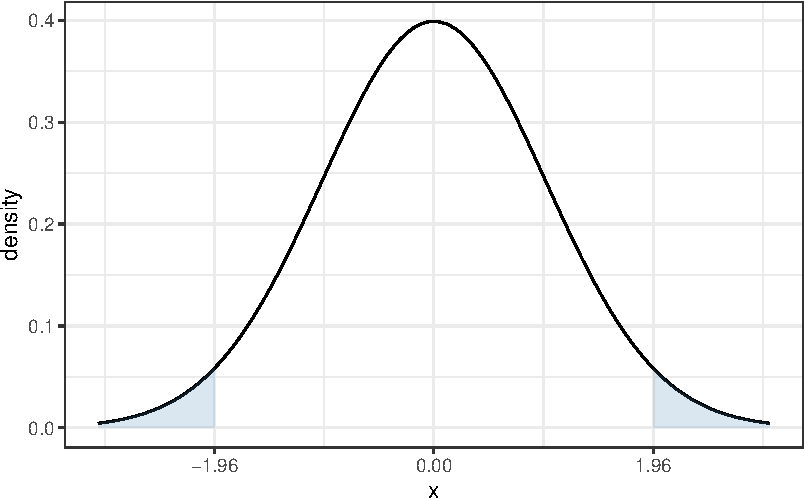
\includegraphics{07-inference_files/figure-pdf/unnamed-chunk-2-1.pdf}

The sum of the two blue, shaded areas is 0.05. In other words, under
\(H_0\), there is a 5\% chance that, by chance, \(t\) would fall in the
shaded areas. If you want to change the significance level, it would
result in a corresponding change in the critical value so that the area
in the new shaded region would adjust too. For example, if you set the
significance level to be \(\alpha=0.1\), then you would need to adjust
the critical value to be 1.64, and if you set \(\alpha=0.01\), then you
would need to adjust the critical value to be 2.58.

\section{P-values}\label{p-values}

Choosing a significance level is somewhat arbitrary. What did we choose
5\%?

Perhaps more importantly, we are essentially throwing away a lot of
information if we are to reduce the information from standard
errors/t-statistics to a binary ``reject'' or ``fail to reject''.

One alternative is to report a \textbf{p-value}. A p-value is the
probability of observing a t-statistic as ``extreme'' as we did if
\(H_0\) were true.

Here is an example of how to calculate a p-value. Suppose we calculate
\(t=1.85\). Then,

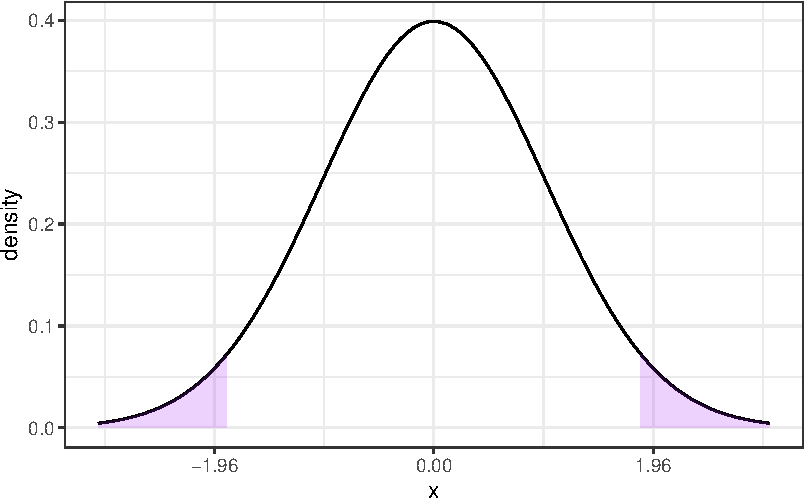
\includegraphics{07-inference_files/figure-pdf/unnamed-chunk-3-1.pdf}

Then, under \(H_0\), the probability of getting a t-statistic ``as
extreme'' as 1.85 corresponds to the area of the two shaded regions
above. In other words, we need to to compute

\[
  \textrm{p-value} = \P(Z \leq -1.85) + \P(Z \geq 1.85)
\] where \(Z \sim N(0,1)\). One thing that is helpful to notice here is
that, a standard normal random variable is symmetric. This means that
\(\P(Z \leq -1.85) = \P(Z \geq 1.85)\). We also typically denote the cdf
of a standard normal random variable with the symbol \(\Phi\). Thus,

\[
  \textrm{p-value} = 2 \Phi(-1.85)
\] I don't know what this is off the top of my head, but it is easy to
compute from a table or using \texttt{R}. In \texttt{R}, you can use the
function \texttt{pnorm} --- here, the p-value is given by
\texttt{2*pnorm(-1.85)} which is equal to 0.064.

More generally, if you calculate a t-statistic, \(t\), using your data
and under \(H_0\), then,

\[
  \textrm{p-value} = 2 \Phi(-|t|)
\]

\section{Confidence Interval}\label{confidence-interval}

Another idea is to report a \((1-\alpha)\%\) (e.g., 95\%) confidence
interval.

The interpretation of a confidence interval is a bit subtle. It is this:
if we collected a large number of samples, and computed a confidence
interval each time, 95\% of these would contain the true value. This is
subtly different than: there is a 95\% probability that \(\theta\) (the
population parameter of interest) falls within the confidence interval
--- this second interpretation doesn't make sense because \(\theta\) is
non-random.

A 95\% confidence interval is given by

\[
  CI_{95\%} = \left[\hat{\theta} - 1.96 \ \textrm{s.e.}(\hat{\theta}), \hat{\theta} + 1.96 \  \textrm{s.e.}(\hat{\theta})\right]
\]

For the particular case where we are interested in \(\E[Y]\), this
becomes

\[
  CI_{95\%} = \left[ \bar{Y} - 1.96 \ \textrm{s.e.}(\bar{Y}), \bar{Y} + 1.96 \ \textrm{s.e.}(\bar{Y}) \right]
\]

\section{Inference in Practice}\label{inference-in-practice}

I have covered the main approaches to inference in this section. I'd
like to make a couple of concluding comments. First, all of the
approaches discussed here (standard errors, t-statistics, p-values, and
confidence intervals) are very closely related (in some sense, they are
just alternative ways to report the same information). They all rely
heavily on establishing asymptotic normality of the estimate of the
parameter of interest --- in fact, this is why we were interested in
asymptotic normality in the first place. My sense is that the most
common thing to report (at least in economics) is an estimate of the
parameter of interest (e.g., \(\hat{\theta}\) or \(\bar{Y}\)) along with
its standard error. If you know this information, you (or your reader)
can easily compute any of the other expressions that we've considered in
this section.

Another important thing to mention is that there is often a distinction
between \textbf{statistical significance} and \textbf{economic
significance}.

In the next chapter, we'll start to think about the \emph{effect} of one
variable on another (e.g., the effect of some economic policy on some
outcome of interest). By far the most common null hypothesis in this
case is that ``the effect'' is equal to 0. However, in economics/social
sciences/business applications, there probably aren't too many cases
where (i) it would be interesting enough to consider the effect of one
variable on another (ii) while simultaneously the effect is literally
equal to 0. Since, all else equal, standard errors get smaller with more
observations, as datasets in economics tend to get larger over time, we
tend to find more statistically significant effects. This doesn't mean
that effects are getting bigger or more important --- just that we are
able to detect smaller and smaller effects if we have enough data. And
most questions in economics involve more than just answering the binary
question: does variable \(X\) have any effect at all on variable \(Y\)?
For example, if you are trying to evaluate the effect of some economic
policy, it is usually more helpful to think in terms of a cost-benefit
analysis --- what are the benefits or the policy relative to the costs
and these sorts of comparisons inherently involve thinking about
magnitudes of effects.

A more succinct way to say all this is: the effect of one variable on
another can be both ``statistically significant'' and ``economically''
small at the same time. Alternatively, if you do not have much data or
the data is very ``noisy'', it may be possible that there are relatively
large effects, but that the estimates are not statistically significant
(i.e., you are not able to detect them very well with the data that you
have). Therefore, it is important to not become too fixated on
statistical significance and to additionally think carefully about the
magnitudes of estimates.

\section{Coding}\label{coding-1}

In this section, we'll use the \texttt{acs} data to calculate an
estimate of average wage/salary income among employed individuals in the
United States. We'll test the null hypothesis that the mean income in
the United States is \$50,000 as well as report the standard error of
our estimate of mean income, as well as corresponding p-values,
t-statistics, and 95\% confidence interval. Finally, we'll report a
table of summary statistics using the \texttt{modelsummary} package
separately by college graduates relative to non-college graduates.

\begin{Shaded}
\begin{Highlighting}[]
\FunctionTok{load}\NormalTok{(}\StringTok{"data/acs.RData"}\NormalTok{)}

\CommentTok{\# estimate of mean income}
\NormalTok{ybar }\OtherTok{\textless{}{-}} \FunctionTok{mean}\NormalTok{(acs}\SpecialCharTok{$}\NormalTok{incwage)}
\NormalTok{ybar}
\end{Highlighting}
\end{Shaded}

\begin{verbatim}
[1] 59263.46
\end{verbatim}

\begin{Shaded}
\begin{Highlighting}[]
\CommentTok{\# calculate standard error}
\NormalTok{V }\OtherTok{\textless{}{-}} \FunctionTok{var}\NormalTok{(acs}\SpecialCharTok{$}\NormalTok{incwage)}
\NormalTok{n }\OtherTok{\textless{}{-}} \FunctionTok{nrow}\NormalTok{(acs)}
\NormalTok{se }\OtherTok{\textless{}{-}} \FunctionTok{sqrt}\NormalTok{(V) }\SpecialCharTok{/} \FunctionTok{sqrt}\NormalTok{(n)}
\NormalTok{se}
\end{Highlighting}
\end{Shaded}

\begin{verbatim}
[1] 713.8138
\end{verbatim}

\begin{Shaded}
\begin{Highlighting}[]
\CommentTok{\# calculate t{-}statistic}
\NormalTok{t\_stat }\OtherTok{\textless{}{-}}\NormalTok{ (ybar }\SpecialCharTok{{-}} \DecValTok{50000}\NormalTok{) }\SpecialCharTok{/}\NormalTok{ se}
\NormalTok{t\_stat}
\end{Highlighting}
\end{Shaded}

\begin{verbatim}
[1] 12.97742
\end{verbatim}

This clearly exceeds 1.96 (or any common critical value) which implies
that we would reject the null hypothesis that mean income is equal to
\$50,000.

\begin{Shaded}
\begin{Highlighting}[]
\CommentTok{\# calculate p{-}value}
\NormalTok{p\_val }\OtherTok{\textless{}{-}} \DecValTok{2}\SpecialCharTok{*}\FunctionTok{pnorm}\NormalTok{(}\SpecialCharTok{{-}}\FunctionTok{abs}\NormalTok{(t\_stat))}
\end{Highlighting}
\end{Shaded}

The p-value is essentially equal to 0. This is expected given the value
of the t-statistic that we calculated earlier.

\begin{Shaded}
\begin{Highlighting}[]
\CommentTok{\# 95\% confidence interval}
\NormalTok{ci\_L }\OtherTok{\textless{}{-}}\NormalTok{ ybar }\SpecialCharTok{{-}} \FloatTok{1.96}\SpecialCharTok{*}\NormalTok{se}
\NormalTok{ci\_U }\OtherTok{\textless{}{-}}\NormalTok{ ybar }\SpecialCharTok{+} \FloatTok{1.96}\SpecialCharTok{*}\NormalTok{se}
\FunctionTok{paste0}\NormalTok{(}\StringTok{"["}\NormalTok{,}\FunctionTok{round}\NormalTok{(ci\_L,}\DecValTok{1}\NormalTok{),}\StringTok{","}\NormalTok{,}\FunctionTok{round}\NormalTok{(ci\_U,}\DecValTok{1}\NormalTok{),}\StringTok{"]"}\NormalTok{)}
\end{Highlighting}
\end{Shaded}

\begin{verbatim}
[1] "[57864.4,60662.5]"
\end{verbatim}

\begin{Shaded}
\begin{Highlighting}[]
\FunctionTok{library}\NormalTok{(modelsummary)}
\end{Highlighting}
\end{Shaded}

\begin{verbatim}
`modelsummary` 2.0.0 now uses `tinytable` as its default table-drawing
  backend. Learn more at: https://vincentarelbundock.github.io/tinytable/

Revert to `kableExtra` for one session:

  options(modelsummary_factory_default = 'kableExtra')
  options(modelsummary_factory_latex = 'kableExtra')
  options(modelsummary_factory_html = 'kableExtra')

Silence this message forever:

  config_modelsummary(startup_message = FALSE)
\end{verbatim}

\begin{Shaded}
\begin{Highlighting}[]
\FunctionTok{library}\NormalTok{(dplyr)}
\end{Highlighting}
\end{Shaded}

\begin{verbatim}

Attaching package: 'dplyr'
\end{verbatim}

\begin{verbatim}
The following objects are masked from 'package:stats':

    filter, lag
\end{verbatim}

\begin{verbatim}
The following objects are masked from 'package:base':

    intersect, setdiff, setequal, union
\end{verbatim}

\begin{Shaded}
\begin{Highlighting}[]
\CommentTok{\# create a factor variable for going to college}
\NormalTok{acs}\SpecialCharTok{$}\NormalTok{col }\OtherTok{\textless{}{-}} \FunctionTok{ifelse}\NormalTok{(acs}\SpecialCharTok{$}\NormalTok{educ }\SpecialCharTok{\textgreater{}=} \DecValTok{16}\NormalTok{, }\StringTok{"college"}\NormalTok{, }\StringTok{"non{-}college"}\NormalTok{)}
\NormalTok{acs}\SpecialCharTok{$}\NormalTok{col }\OtherTok{\textless{}{-}} \FunctionTok{as.factor}\NormalTok{(acs}\SpecialCharTok{$}\NormalTok{col)}
\NormalTok{acs}\SpecialCharTok{$}\NormalTok{female }\OtherTok{\textless{}{-}} \DecValTok{1}\SpecialCharTok{*}\NormalTok{(acs}\SpecialCharTok{$}\NormalTok{sex}\SpecialCharTok{==}\DecValTok{2}\NormalTok{)}
\NormalTok{acs}\SpecialCharTok{$}\NormalTok{incwage }\OtherTok{\textless{}{-}}\NormalTok{ acs}\SpecialCharTok{$}\NormalTok{incwage}\SpecialCharTok{/}\DecValTok{1000}
\FunctionTok{datasummary\_balance}\NormalTok{(}\SpecialCharTok{\textasciitilde{}}\NormalTok{ col, }\AttributeTok{data=}\NormalTok{dplyr}\SpecialCharTok{::}\FunctionTok{select}\NormalTok{(acs, incwage, female, age, col),}
                    \AttributeTok{fmt=}\DecValTok{2}\NormalTok{)}
\end{Highlighting}
\end{Shaded}

\begin{table}
\centering
\begin{tblr}[         %% tabularray outer open
]                     %% tabularray outer close
{                     %% tabularray inner open
colspec={Q[]Q[]Q[]Q[]Q[]Q[]Q[]},
cell{1}{2}={c=2,}{halign=c,},
cell{1}{4}={c=2,}{halign=c,},
column{1}={halign=l,},
column{2}={halign=r,},
column{3}={halign=r,},
column{4}={halign=r,},
column{5}={halign=r,},
column{6}={halign=r,},
column{7}={halign=r,},
row{1}={halign=c,},
}                     %% tabularray inner close
\toprule
& college (N=3871) &  & non-college (N=6129) &  &  &  \\ \cmidrule[lr]{2-3}\cmidrule[lr]{4-5}
& Mean & Std. Dev. & Mean & Std. Dev. & Diff. in Means & Std. Error \\ \midrule %% TinyTableHeader
incwage & \num{89.69} & \num{96.15} & \num{40.05} & \num{39.01} & \num{-49.65} & \num{1.62} \\
female  & \num{0.51}  & \num{0.50}  & \num{0.46}  & \num{0.50}  & \num{-0.04}  & \num{0.01} \\
age     & \num{44.38} & \num{13.43} & \num{42.80} & \num{15.71} & \num{-1.58}  & \num{0.29} \\
\bottomrule
\end{tblr}
\end{table}

\section{Lab 3: Monte Carlo
Simulations}\label{lab-3-monte-carlo-simulations}

In this lab, we will study the theoretical properties of the estimators
that we have been discussing in this chapter.

\textbf{Monte Carlo simulations} are a useful way to study/understand
the properties of an estimation procedure. The basic idea is that,
instead of using real data, we are going to use simulated data where we
control the data generating process. This will be useful for two
reasons. First, we will \emph{know} what \textbf{the truth} is and
compare results coming from our estimation procedure to the truth.
Second, because we are simulating data, we can actually carry out our
thought experiment of repeatedly drawing a sample of some particular
size.

For this lab, we are going to make simulated coin flips.

\begin{enumerate}
\def\labelenumi{\arabic{enumi}.}
\item
  Write a function called \texttt{flip} that takes in an argument
  \texttt{p} where \texttt{p} stands for the probability of flipping a
  heads (you can code this as a \texttt{1} and \texttt{0} for tails) and
  outputs either \texttt{1} or \texttt{0}. Run the code

\begin{verbatim}
flip(0.5)
\end{verbatim}

  \textbf{Hint:} It may be helpful to use the \texttt{R} function
  \texttt{sample}.
\item
  Write a function called \texttt{generate\_sample} that takes in the
  arguments \texttt{n} and \texttt{p} and generates a sample of
  \texttt{n} coin flips where the probability of flipping heads is
  \texttt{p}. Run the code

\begin{verbatim}
generate_sample(10,0.5)
\end{verbatim}
\item
  Next, over 1000 Monte Carlo simulations (i.e., do the following 1000
  times),

  \begin{enumerate}
  \def\labelenumii{(\roman{enumii})}
  \item
    generate a new sample with 10 observations
  \item
    calculate an estimate of \(p\)
  \end{enumerate}

  (\textbf{Hint:} you can estimate \(p\) by just calculating the average
  number of heads flipped in a particular simulation)

  \begin{enumerate}
  \def\labelenumii{(\roman{enumii})}
  \setcounter{enumii}{2}
  \item
    a t-statistic for the null hypothesis that \(p=0.5\)
  \item
    and record whether or not you reject the null hypothesis that
    \(p=0.5\) in that simulation
  \end{enumerate}
\end{enumerate}

Then, using all 1000 Monte Carlo simulations, report (i) an estimate of
the bias of your estimator, (ii) an estimate of the variance of your
estimator, (iii) an estimate of the mean squared error of your
estimator, (iv) plot a histogram of the t-statistics across iterations,
and (v) report the fraction of times that you reject \(H_0\).

\begin{enumerate}
\def\labelenumi{\arabic{enumi}.}
\setcounter{enumi}{3}
\item
  Same as \#3, but with 50 observations in each simulation. What
  differences do you notice?
\item
  Same as \#3, but with 50 observations and test \(H_0:p=0.6\). What
  differences do you notice?
\item
  Same as \#3, but with 50 observations and test \(H_0:p=0.9\). What
  differences do you notice?
\item
  Same as \#3, but with 1000 observations and test \(H_0:p=0.6\). What
  differences do you notice?
\item
  Same as \#3, but now set \(p=0.95\) (so that this is an unfair coin
  that flips heads 95\% of the time) and with 10 observations and test
  \(H_0:p=0.95\). What differences do you notice?
\item
  Same as \#8, but with 50 observations. What differences do you notice?
\item
  Same as \#8, but with 1000 observations. What differences do you
  notice?
\end{enumerate}

\textbf{Hint:} Since problems 3-10 ask you to do roughly the same thing
over and over, it is probably useful to try to write a function to do
all of these but with arguments that allow you to change the number of
observations per simulation, the true value of \(p\), and the null
hypothesis that you are testing.

\section{Lab 3 Solutions}\label{lab-3-solutions}

\begin{enumerate}
\def\labelenumi{\arabic{enumi}.}
\tightlist
\item
\end{enumerate}

\begin{Shaded}
\begin{Highlighting}[]
\CommentTok{\# function to flip a coin with probability p}
\NormalTok{flip }\OtherTok{\textless{}{-}} \ControlFlowTok{function}\NormalTok{(p) \{}
  \FunctionTok{sample}\NormalTok{(}\FunctionTok{c}\NormalTok{(}\DecValTok{0}\NormalTok{,}\DecValTok{1}\NormalTok{), }\AttributeTok{size=}\DecValTok{1}\NormalTok{, }\AttributeTok{prob=}\NormalTok{(}\FunctionTok{c}\NormalTok{(}\DecValTok{1}\SpecialCharTok{{-}}\NormalTok{p,p)))}
\NormalTok{\}}

\CommentTok{\# test out flip function}
\FunctionTok{flip}\NormalTok{(}\FloatTok{0.5}\NormalTok{)}
\end{Highlighting}
\end{Shaded}

\begin{verbatim}
[1] 0
\end{verbatim}

\begin{enumerate}
\def\labelenumi{\arabic{enumi}.}
\setcounter{enumi}{1}
\tightlist
\item
\end{enumerate}

\begin{Shaded}
\begin{Highlighting}[]
\CommentTok{\# function to generate a sample of size n}
\NormalTok{generate\_sample }\OtherTok{\textless{}{-}} \ControlFlowTok{function}\NormalTok{(n,p) \{}
\NormalTok{  Y }\OtherTok{\textless{}{-}} \FunctionTok{c}\NormalTok{()}
  \ControlFlowTok{for}\NormalTok{ (i }\ControlFlowTok{in} \DecValTok{1}\SpecialCharTok{:}\NormalTok{n) \{}
\NormalTok{    Y[i] }\OtherTok{\textless{}{-}} \FunctionTok{flip}\NormalTok{(p)}
\NormalTok{  \}}
\NormalTok{  Y}
\NormalTok{\}}

\CommentTok{\# test out generate\_sample function}
\FunctionTok{generate\_sample}\NormalTok{(}\DecValTok{10}\NormalTok{,}\FloatTok{0.5}\NormalTok{)}
\end{Highlighting}
\end{Shaded}

\begin{verbatim}
 [1] 1 0 0 1 0 0 0 0 0 0
\end{verbatim}

\begin{enumerate}
\def\labelenumi{\arabic{enumi}.}
\setcounter{enumi}{2}
\tightlist
\item
\end{enumerate}

\begin{Shaded}
\begin{Highlighting}[]
\CommentTok{\# carry out monte carlo simulations}
\NormalTok{n }\OtherTok{\textless{}{-}} \DecValTok{10}
\NormalTok{p }\OtherTok{\textless{}{-}} \FloatTok{0.5}
\NormalTok{nsims }\OtherTok{\textless{}{-}} \DecValTok{1000}  \CommentTok{\# need to pick large number of monte carlo simulations}
\NormalTok{mc\_est }\OtherTok{\textless{}{-}} \FunctionTok{c}\NormalTok{()  }\CommentTok{\# vector to hold estimation results}
\NormalTok{mc\_var }\OtherTok{\textless{}{-}} \FunctionTok{c}\NormalTok{()  }\CommentTok{\# vector to hold estimated variance}

\ControlFlowTok{for}\NormalTok{ (i }\ControlFlowTok{in} \DecValTok{1}\SpecialCharTok{:}\NormalTok{nsims) \{}
\NormalTok{  Y }\OtherTok{\textless{}{-}} \FunctionTok{generate\_sample}\NormalTok{(n,p)}
\NormalTok{  mc\_est[i] }\OtherTok{\textless{}{-}} \FunctionTok{mean}\NormalTok{(Y)}
\NormalTok{  mc\_var[i] }\OtherTok{\textless{}{-}} \FunctionTok{var}\NormalTok{(Y)}
\NormalTok{\}}

\CommentTok{\# compute bias}
\NormalTok{bias }\OtherTok{\textless{}{-}} \FunctionTok{mean}\NormalTok{(mc\_est) }\SpecialCharTok{{-}}\NormalTok{ p}
\NormalTok{bias}
\end{Highlighting}
\end{Shaded}

\begin{verbatim}
[1] -0.0086
\end{verbatim}

\begin{Shaded}
\begin{Highlighting}[]
\CommentTok{\# compute sampling variance}
\NormalTok{var }\OtherTok{\textless{}{-}} \FunctionTok{var}\NormalTok{(mc\_est)}
\NormalTok{var}
\end{Highlighting}
\end{Shaded}

\begin{verbatim}
[1] 0.02575179
\end{verbatim}

\begin{Shaded}
\begin{Highlighting}[]
\CommentTok{\# compute mean squared error}
\NormalTok{mse }\OtherTok{\textless{}{-}}\NormalTok{ bias}\SpecialCharTok{\^{}}\DecValTok{2} \SpecialCharTok{+}\NormalTok{ var}
\NormalTok{mse}
\end{Highlighting}
\end{Shaded}

\begin{verbatim}
[1] 0.02582575
\end{verbatim}

\begin{Shaded}
\begin{Highlighting}[]
\NormalTok{H0 }\OtherTok{\textless{}{-}}\NormalTok{ p}
\NormalTok{t }\OtherTok{\textless{}{-}} \FunctionTok{sqrt}\NormalTok{(n)}\SpecialCharTok{*}\NormalTok{(mc\_est }\SpecialCharTok{{-}}\NormalTok{ H0) }\SpecialCharTok{/} \FunctionTok{sqrt}\NormalTok{(mc\_var)}
\FunctionTok{ggplot}\NormalTok{(}\FunctionTok{data.frame}\NormalTok{(}\AttributeTok{t=}\NormalTok{t), }\FunctionTok{aes}\NormalTok{(}\AttributeTok{x=}\NormalTok{t)) }\SpecialCharTok{+}
  \FunctionTok{geom\_histogram}\NormalTok{(}\AttributeTok{bins=}\DecValTok{30}\NormalTok{) }\SpecialCharTok{+}
  \FunctionTok{theme\_bw}\NormalTok{()}
\end{Highlighting}
\end{Shaded}

\begin{verbatim}
Warning: Removed 1 row containing non-finite outside the scale range
(`stat_bin()`).
\end{verbatim}

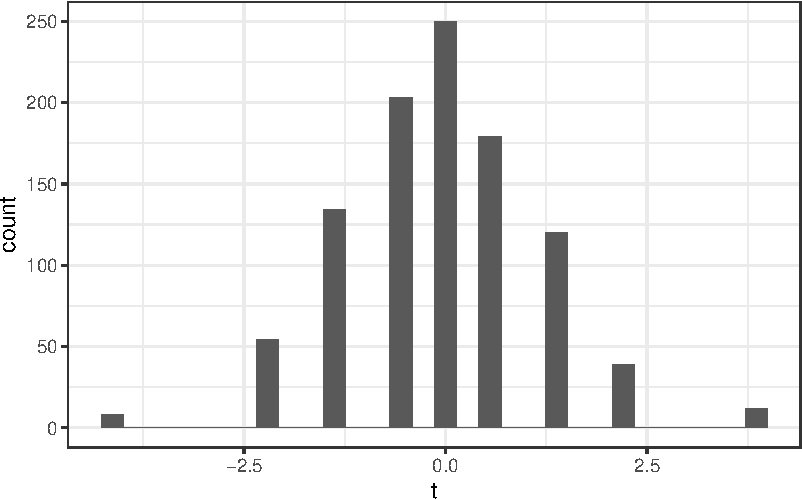
\includegraphics{07-inference_files/figure-pdf/unnamed-chunk-10-1.pdf}

\begin{Shaded}
\begin{Highlighting}[]
\NormalTok{rej }\OtherTok{\textless{}{-}} \FunctionTok{mean}\NormalTok{(}\DecValTok{1}\SpecialCharTok{*}\NormalTok{(}\FunctionTok{abs}\NormalTok{(t) }\SpecialCharTok{\textgreater{}=} \FloatTok{1.96}\NormalTok{))}
\NormalTok{rej}
\end{Highlighting}
\end{Shaded}

\begin{verbatim}
[1] 0.114
\end{verbatim}

\begin{enumerate}
\def\labelenumi{\arabic{enumi}.}
\setcounter{enumi}{3}
\tightlist
\item
\end{enumerate}

\begin{Shaded}
\begin{Highlighting}[]
\CommentTok{\# since we are going to do this over and over, let\textquotesingle{}s write a function to do it}
\NormalTok{mc\_sim }\OtherTok{\textless{}{-}} \ControlFlowTok{function}\NormalTok{(n, p, H0) \{}
\NormalTok{  mc\_est }\OtherTok{\textless{}{-}} \FunctionTok{c}\NormalTok{()  }\CommentTok{\# vector to hold estimation results}
\NormalTok{  mc\_var }\OtherTok{\textless{}{-}} \FunctionTok{c}\NormalTok{()  }\CommentTok{\# vector to hold estimated variance}

  \ControlFlowTok{for}\NormalTok{ (i }\ControlFlowTok{in} \DecValTok{1}\SpecialCharTok{:}\NormalTok{nsims) \{}
\NormalTok{    Y }\OtherTok{\textless{}{-}} \FunctionTok{generate\_sample}\NormalTok{(n,p)}
\NormalTok{    mc\_est[i] }\OtherTok{\textless{}{-}} \FunctionTok{mean}\NormalTok{(Y)}
\NormalTok{    mc\_var[i] }\OtherTok{\textless{}{-}} \FunctionTok{var}\NormalTok{(Y)}
\NormalTok{  \}}

  \CommentTok{\# compute bias}
\NormalTok{  bias }\OtherTok{\textless{}{-}} \FunctionTok{mean}\NormalTok{(mc\_est) }\SpecialCharTok{{-}}\NormalTok{ p}

  \CommentTok{\# compute sampling variance}
\NormalTok{  var }\OtherTok{\textless{}{-}} \FunctionTok{var}\NormalTok{(mc\_est)}

  \CommentTok{\# compute mean squared error}
\NormalTok{  mse }\OtherTok{\textless{}{-}}\NormalTok{ bias}\SpecialCharTok{\^{}}\DecValTok{2} \SpecialCharTok{+}\NormalTok{ var}
  
\NormalTok{  t }\OtherTok{\textless{}{-}} \FunctionTok{sqrt}\NormalTok{(n)}\SpecialCharTok{*}\NormalTok{(mc\_est }\SpecialCharTok{{-}}\NormalTok{ H0) }\SpecialCharTok{/} \FunctionTok{sqrt}\NormalTok{(mc\_var)}
\NormalTok{  hist\_plot }\OtherTok{\textless{}{-}} \FunctionTok{ggplot}\NormalTok{(}\FunctionTok{data.frame}\NormalTok{(}\AttributeTok{t=}\NormalTok{t), }\FunctionTok{aes}\NormalTok{(}\AttributeTok{x=}\NormalTok{t)) }\SpecialCharTok{+}
    \FunctionTok{geom\_histogram}\NormalTok{(}\AttributeTok{bins=}\DecValTok{30}\NormalTok{) }\SpecialCharTok{+} 
    \FunctionTok{theme\_bw}\NormalTok{()}

\NormalTok{  rej }\OtherTok{\textless{}{-}} \FunctionTok{mean}\NormalTok{(}\DecValTok{1}\SpecialCharTok{*}\NormalTok{(}\FunctionTok{abs}\NormalTok{(t) }\SpecialCharTok{\textgreater{}=} \FloatTok{1.96}\NormalTok{))}
  
  \CommentTok{\# print results}
  \FunctionTok{print}\NormalTok{(}\FunctionTok{paste0}\NormalTok{(}\StringTok{"bias: "}\NormalTok{, }\FunctionTok{round}\NormalTok{(bias,}\DecValTok{4}\NormalTok{)))}
  \FunctionTok{print}\NormalTok{(}\FunctionTok{paste0}\NormalTok{(}\StringTok{"var : "}\NormalTok{, }\FunctionTok{round}\NormalTok{(var,}\DecValTok{4}\NormalTok{)))}
  \FunctionTok{print}\NormalTok{(}\FunctionTok{paste0}\NormalTok{(}\StringTok{"mse : "}\NormalTok{, }\FunctionTok{round}\NormalTok{(mse,}\DecValTok{4}\NormalTok{)))}
  \FunctionTok{print}\NormalTok{(hist\_plot)}
  \FunctionTok{print}\NormalTok{(}\FunctionTok{paste0}\NormalTok{(}\StringTok{"rej : "}\NormalTok{, }\FunctionTok{round}\NormalTok{(rej,}\DecValTok{4}\NormalTok{)))}
\NormalTok{\}}
\FunctionTok{mc\_sim}\NormalTok{(}\DecValTok{50}\NormalTok{, }\FloatTok{0.5}\NormalTok{, }\FloatTok{0.5}\NormalTok{)}
\end{Highlighting}
\end{Shaded}

\begin{verbatim}
[1] "bias: 0.0028"
[1] "var : 0.0052"
[1] "mse : 0.0053"
\end{verbatim}

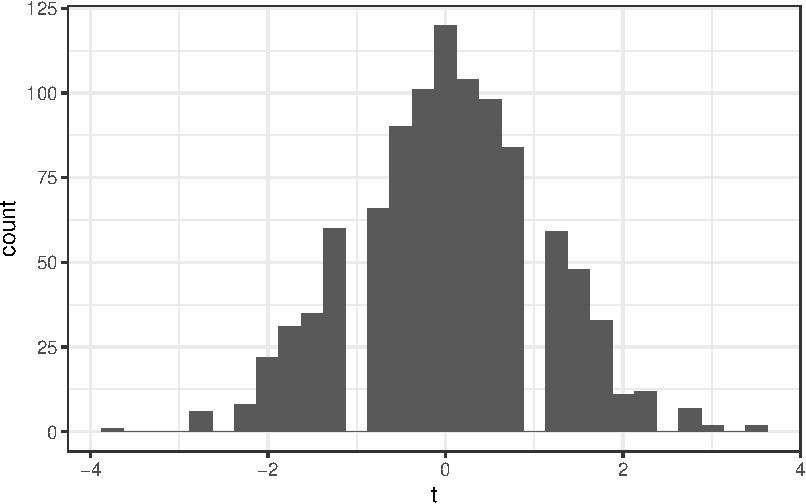
\includegraphics{07-inference_files/figure-pdf/unnamed-chunk-11-1.pdf}

\begin{verbatim}
[1] "rej : 0.071"
\end{verbatim}

\begin{enumerate}
\def\labelenumi{\arabic{enumi}.}
\setcounter{enumi}{4}
\tightlist
\item
\end{enumerate}

\begin{Shaded}
\begin{Highlighting}[]
\FunctionTok{mc\_sim}\NormalTok{(}\DecValTok{50}\NormalTok{, }\FloatTok{0.5}\NormalTok{, }\FloatTok{0.6}\NormalTok{)}
\end{Highlighting}
\end{Shaded}

\begin{verbatim}
[1] "bias: -0.0018"
[1] "var : 0.005"
[1] "mse : 0.005"
\end{verbatim}

\includegraphics{07-inference_files/figure-pdf/unnamed-chunk-12-1.pdf}

\begin{verbatim}
[1] "rej : 0.362"
\end{verbatim}

\begin{enumerate}
\def\labelenumi{\arabic{enumi}.}
\setcounter{enumi}{5}
\tightlist
\item
\end{enumerate}

\begin{Shaded}
\begin{Highlighting}[]
\FunctionTok{mc\_sim}\NormalTok{(}\DecValTok{50}\NormalTok{, }\FloatTok{0.5}\NormalTok{, }\FloatTok{0.9}\NormalTok{)}
\end{Highlighting}
\end{Shaded}

\begin{verbatim}
[1] "bias: 0.004"
[1] "var : 0.0048"
[1] "mse : 0.0048"
\end{verbatim}

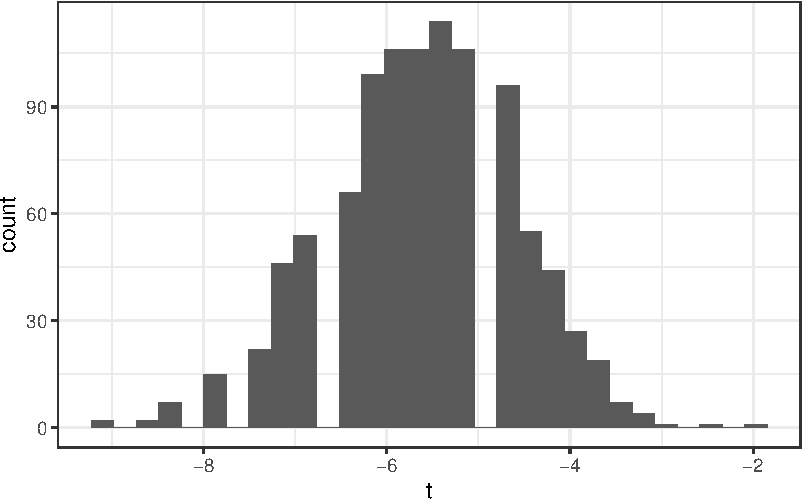
\includegraphics{07-inference_files/figure-pdf/unnamed-chunk-13-1.pdf}

\begin{verbatim}
[1] "rej : 1"
\end{verbatim}

\begin{enumerate}
\def\labelenumi{\arabic{enumi}.}
\setcounter{enumi}{6}
\tightlist
\item
\end{enumerate}

\begin{Shaded}
\begin{Highlighting}[]
\FunctionTok{mc\_sim}\NormalTok{(}\DecValTok{1000}\NormalTok{, }\FloatTok{0.5}\NormalTok{, }\FloatTok{0.6}\NormalTok{)}
\end{Highlighting}
\end{Shaded}

\begin{verbatim}
[1] "bias: -5e-04"
[1] "var : 3e-04"
[1] "mse : 3e-04"
\end{verbatim}

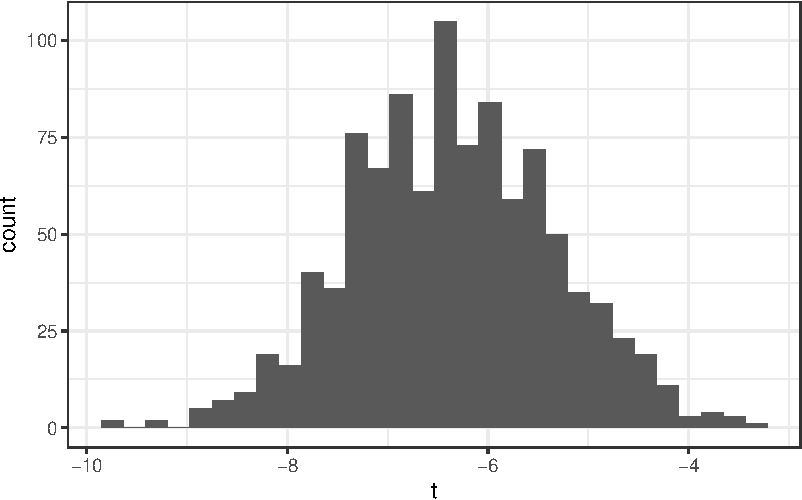
\includegraphics{07-inference_files/figure-pdf/unnamed-chunk-14-1.pdf}

\begin{verbatim}
[1] "rej : 1"
\end{verbatim}

\begin{enumerate}
\def\labelenumi{\arabic{enumi}.}
\setcounter{enumi}{7}
\tightlist
\item
\end{enumerate}

\begin{Shaded}
\begin{Highlighting}[]
\FunctionTok{mc\_sim}\NormalTok{(}\DecValTok{10}\NormalTok{, }\FloatTok{0.95}\NormalTok{, }\FloatTok{0.95}\NormalTok{)}
\end{Highlighting}
\end{Shaded}

\begin{verbatim}
[1] "bias: 0.002"
[1] "var : 0.0044"
[1] "mse : 0.0044"
\end{verbatim}

\begin{verbatim}
Warning: Removed 606 rows containing non-finite outside the scale range
(`stat_bin()`).
\end{verbatim}

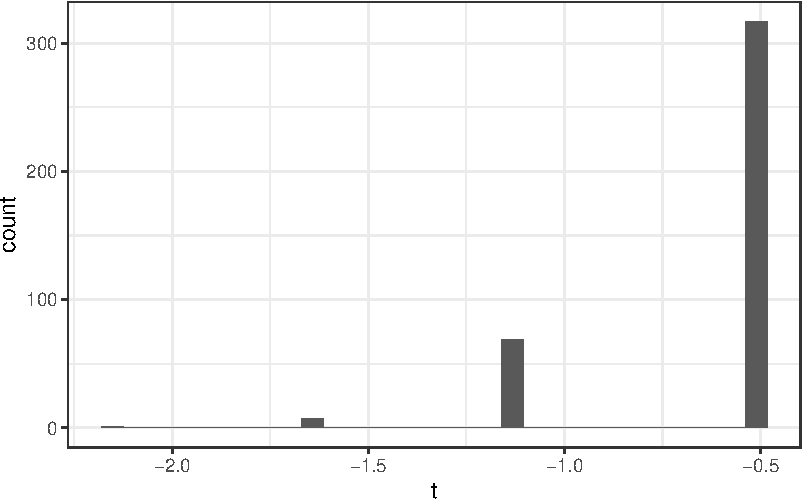
\includegraphics{07-inference_files/figure-pdf/unnamed-chunk-15-1.pdf}

\begin{verbatim}
[1] "rej : 0.607"
\end{verbatim}

\begin{enumerate}
\def\labelenumi{\arabic{enumi}.}
\setcounter{enumi}{8}
\tightlist
\item
\end{enumerate}

\begin{Shaded}
\begin{Highlighting}[]
\FunctionTok{mc\_sim}\NormalTok{(}\DecValTok{50}\NormalTok{, }\FloatTok{0.95}\NormalTok{, }\FloatTok{0.95}\NormalTok{)}
\end{Highlighting}
\end{Shaded}

\begin{verbatim}
[1] "bias: -5e-04"
[1] "var : 9e-04"
[1] "mse : 9e-04"
\end{verbatim}

\begin{verbatim}
Warning: Removed 70 rows containing non-finite outside the scale range
(`stat_bin()`).
\end{verbatim}

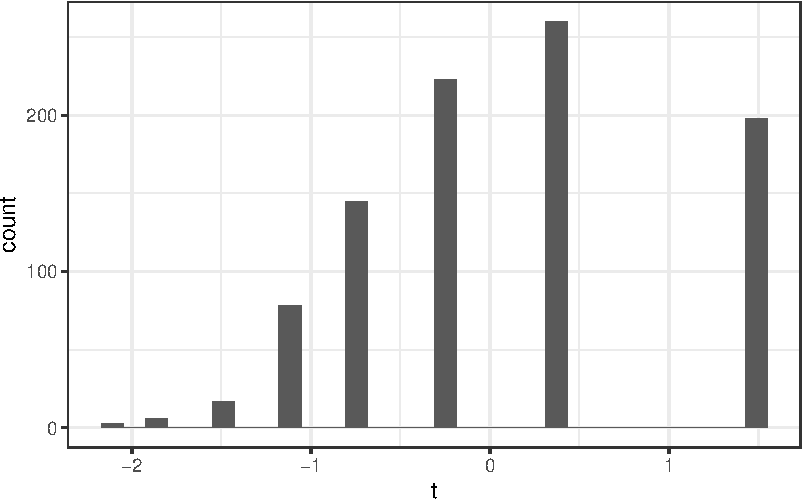
\includegraphics{07-inference_files/figure-pdf/unnamed-chunk-16-1.pdf}

\begin{verbatim}
[1] "rej : 0.073"
\end{verbatim}

\begin{enumerate}
\def\labelenumi{\arabic{enumi}.}
\setcounter{enumi}{9}
\tightlist
\item
\end{enumerate}

\begin{Shaded}
\begin{Highlighting}[]
\FunctionTok{mc\_sim}\NormalTok{(}\DecValTok{1000}\NormalTok{, }\FloatTok{0.95}\NormalTok{, }\FloatTok{0.95}\NormalTok{)}
\end{Highlighting}
\end{Shaded}

\begin{verbatim}
[1] "bias: -2e-04"
[1] "var : 0"
[1] "mse : 0"
\end{verbatim}

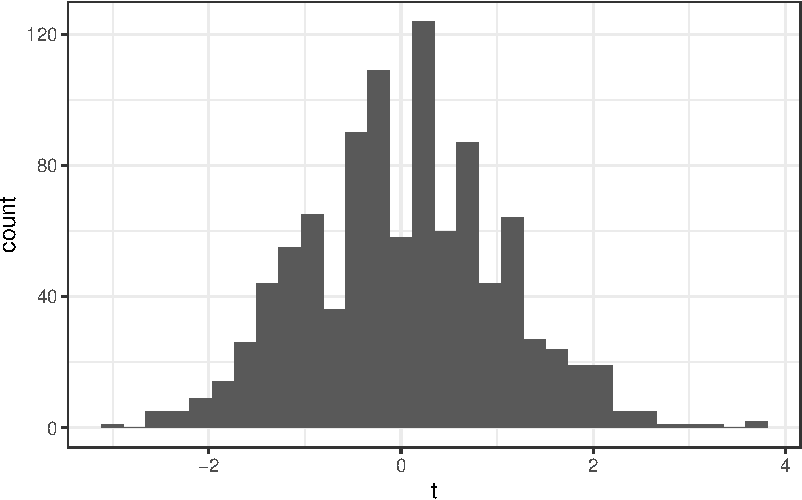
\includegraphics{07-inference_files/figure-pdf/unnamed-chunk-17-1.pdf}

\begin{verbatim}
[1] "rej : 0.054"
\end{verbatim}

\section{Coding Questions}\label{coding-questions-1}

\begin{enumerate}
\def\labelenumi{\arabic{enumi}.}
\item
  For this question, we'll use the data \texttt{Airq}. The variable
  \texttt{rain} contains the amount of rainfall in the county in a year
  (in inches). For this question, we'll be interested in testing whether
  or not the mean rainfall across counties in California is 25 inches.

  \begin{enumerate}
  \def\labelenumii{\alph{enumii})}
  \item
    Estimate the mean rainfall across counties.
  \item
    Calculate the standard error of your estimate of rainfall.
  \item
    Calculate a t-statistic for \(H_0 : \E[Y] = 25\) where \(Y\) denotes
    rainfall. Do you reject \(H_0\) at a 5\% significance level?
    Explain.
  \item
    Calculate a p-value for \(H_0: \E[Y] = 25\). How should you
    interpret this?
  \item
    Calculate a 95\% confidence interval for average rainfall.
  \item
    Use the \texttt{datasummary\_balance} function from the
    \texttt{modelsummary} package to report average air quality, value
    added, rain, population density, and average income, separately by
    whether or not the county is located in a coastal area.
  \end{enumerate}
\end{enumerate}

\section{Extra Questions}\label{extra-questions-1}

\begin{enumerate}
\def\labelenumi{\arabic{enumi}.}
\item
  What is the difference between consistency and unbiasedness?
\item
  Suppose you have an estimator that is unbiased. Will it necessarily be
  consistent? If not, provide an example of an unbiased estimator that
  is not consistent.
\item
  Suppose you have an estimator that is consistent. Will it necessarily
  be unbiased? If not, provide an example of a consistent estimator that
  is not unbiased.
\item
  The Central Limit Theorem says that,
  \(\sqrt{n}\left(\frac{1}{n} \sum_{i=1}^n (Y_i - \E[Y])\right) \rightarrow N(0,V)\)
  as \(n \rightarrow \infty\) where \(V = \var(Y)\).

  \begin{enumerate}
  \def\labelenumii{\alph{enumii})}
  \item
    What happens to
    \(n \left(\frac{1}{n} \sum_{i=1}^n (Y_i - \E[Y])\right)\) as
    \(n \rightarrow \infty\)? Explain.
  \item
    What happens to
    \(n^{1/3} \left(\frac{1}{n} \sum_{i=1}^n (Y_i - \E[Y])\right)\) as
    \(n \rightarrow \infty\)? Explain.
  \end{enumerate}
\end{enumerate}

\part{Regression}

\bookmarksetup{startatroot}

\chapter{Interpreting Regressions}\label{interpreting-regressions}

\[
\newcommand{\E}{\mathbb{E}}
\renewcommand{\P}{\textrm{P}}
\let\L\relax
\newcommand{\L}{\textrm{L}} %doesn't work in .qmd, place this command at start of qmd file to use it
\newcommand{\F}{\textrm{F}}
\newcommand{\var}{\textrm{var}}
\newcommand{\cov}{\textrm{cov}}
\newcommand{\corr}{\textrm{corr}}
\newcommand{\Var}{\mathrm{Var}}
\newcommand{\Cov}{\mathrm{Cov}}
\newcommand{\Corr}{\mathrm{Corr}}
\newcommand{\sd}{\mathrm{sd}}
\newcommand{\se}{\mathrm{s.e.}}
\newcommand{\T}{T}
\newcommand{\indicator}[1]{\mathbb{1}\{#1\}}
\newcommand\independent{\perp \!\!\! \perp}
\newcommand{\N}{\mathcal{N}}
\]

In this chapter, our interest will shift to conditional expectations,
such as \(\E[Y|X_1,X_2,X_3]\) (I'll write \(X_1\), \(X_2\), and \(X_3\)
in a lot of examples in this chapter, but you can think of there being
an arbitrary number of \(X\)'s).

I'll refer to \(Y\) as the \textbf{outcome}. You might also sometimes
heae it called the \textbf{dependent variable}.

I'll refer to the \(X\)'s as either \textbf{covariates} or
\textbf{regressors} or \textbf{characteristics}. You might also hear
them called \textbf{independent variables} sometimes.

Before we start to get into the details, let us first discuss why we're
interested in conditional expectations. First, if we are interested in
\emph{making predictions}, it will often be the case that the ``best''
prediction that one can make is the conditional expectation. This should
make sense to you --- if you want to make a reasonable prediction about
what the outcome will be for a new observation that has characteristics
\(x_1\), \(x_2\), and \(x_3\), a good way to do it would be to predict
that their outcome would be the same as the mean outcome in the
population among those that have the same characteristics; that is,
\(\E[Y|X_1=x_1, X_2=x_2, X_3=x_3]\).

Next, in economics, we are often interested in how much some outcome of
interest changes when a particular covariate changes, holding other
covariates constants. To give some examples, we might be interested in
the average return of actively managed mutual funds relative to
passively managed mutual funds conditional on investing in assets in the
same class (e.g., large cap stocks or international bonds). As another
example, we might be interested in the effect of an increase in the
amount of fertilizer on average crop yield but while holding constant
the temperature and precipitation.

How much the outcome, \(Y\), changes on average when one of the
covariates, \(X_1\), changes by 1 unit and holding other covariates
constant is what we'll call the \textbf{partial effect} of \(X_1\) on
\(Y\). Suppose \(X_1\) is binary, then it is given by

\[
  PE(x_2,x_3) = \E[Y | X_1=1, X_2=x_2, X_3=x_3] - \E[Y | X_1=0,X_2=x_2,X_3=x_3]
\] Notice that the partial effect can depend on \(x_2\) and \(x_3\). For
example, it could be that the effect of active management relative to
passive management could be different across different asset classes.

Slightly more generally, if \(X_1\) is discrete, so that it can take on
several different discrete values, then we define the partial effect as

\[
  PE(x_1,x_2,x_3) = \E[Y | X_1=x_1+1, X_2=x_2, X_3=x_3] - \E[Y | X_1=x_1,X_2=x_2,X_3=x_3]
\] which now can depend on \(x_1\), \(x_2\), and \(x_3\). This is the
average effect of going from \(X_1=x_1\) to \(X_1=x_1+1\) holding
\(x_2\) and \(x_3\) constant.

Finally, consider the case where we are interested in the partial effect
of \(X_1\) which is continuous (for example, the partial effect of
fertilizer input on crop yield). In this case the partial effect is
given by the \emph{partial derivative} of \(\E[Y|X_1,X_2,X_3]\) with
respect to \(X_1\).

\[
  PE(x_1,x_2,x_3) = \frac{\partial \, \E[Y|X_1=x_1, X_2=x_2, X_3=x_3]}{\partial \, x_1}
\] This partial derivative is analogous to what we have been doing
before --- we are making a small change of \(X_1\) while holding \(X_2\)
and \(X_3\) constant at \(x_2\) and \(x_3\).

{Side-Comment:} This is probably the part of the class where we will
jump around in the book the most this semester.

The pedagogical approach of the textbook is to introduce the notion of
causality very early and to emphasize the requirements on linear
regression models in order to deliver causality, while increasing the
complexity of the models over several chapters.

This is totally reasonable, but I prefer to start by teaching the
mechanics of regressions: how to compute them, how to interpret them
(even if you are not able to meet the requirements of causality), and
how to use them to make predictions. Then, we'll have a serious
discussion about causality over the last few weeks of the semester.

In practice, this means we'll cover parts Chapters 4-8 in the textbook
now, and then we'll circle back to some of the issues covered in these
chapters again towards the end of the semester.

\section{Nonparametric Regression / Curse of
Dimensionality}\label{nonparametric-regression-curse-of-dimensionality}

If you knew nothing about regressions, it would seem natural to try to
estimate \(\E[Y|X_1=x_1,X_2=x_2,X_3=x_3]\) by just calculating the
average of \(Y\) among observations that have values of the regressors
equal to \(x_1\), \(x_2\), and \(x_3\) (if these are discrete) or that
are, in some sense, close to \(x_1\), \(x_2\), and \(x_3\) (if these are
continuous).

This is actually a pretty attractive idea.

However, you run into the issue that it is practically challenging to do
this when the number of regressors starts to get large (i.e., if you
have 10 regressors, generally, you would need tons of data to be able to
find a suitable number of observations that are ``close'' to any
particular value of the regressors).

Let me give a more concrete example. Suppose that you were trying to
estimate mean house price as a function of a house's characteristics. If
the only characteristic of the house that you knew was the number of
bedrooms, then it would be pretty easy to just calculate the average
house price among houses with 2, 3, 4, etc. bedrooms. Now suppose that
you knew both the number of bedrooms and the number of square feet. In
this case, if we wanted to estimate mean house prices as a function of
these characteristics, we would need to find houses that have the same
number of bedrooms and (at least) a similar number of square feet. This
starts to ``slice'' the data that you have more thinly. If you continue
with this idea (suppose that you want to estimate mean house price as a
function of number of bedrooms, number of bathrooms, number of square
feet, what year the house was built in, whether or not it has a
basement, what zip code it is located in, etc.) then you will start to
stretch your data extremely thin to the point that you may have very few
relevant observations (or perhaps no relevant observations) for
particular values of the characteristics.

This issue is called the ``curse of dimensionality''.

We will focus on linear models for \(\E[Y|X_1,X_2,X_3]\) largely to get
around the curse of dimensionality.

This idea of using observations that are very close in terms of
characteristics in order to estimate a conditional expectation is called
\textbf{nonparametric} econometrics/statistics. You can take entire
courses (typically graduate-level) on this topic if you were interested.
The reason that it is is called nonparametric is that it doesn't involve
making any functional form assumptions (like linearity) but the cost is
that it would typically require many more observations (due to the curse
of dimensionality).

\section{Linear Regression Models}\label{linear-regression-models}

SW 4.1

In order to get around the curse of dimensionality that we discussed in
the previous section, we will often an impose a \textbf{linear model}
for the conditional expectation. For example,

\[
  \E[Y|X] = \beta_0 + \beta_1 X
\] or

\[
  \E[Y|X_1,X_2,X_3] = \beta_0 + \beta_1 X_1 + \beta_2 X_2 + \beta_3 X_3
\] If we know the values of \(\beta_0\), \(\beta_1\), \(\beta_2\), and
\(\beta_3\), then it is straighforward for us to make predictions. In
particular, suppose that we want to predict the outcome for a new
observation with characteristics \(x_1\), \(x_2\), and \(x_3\). Our
prediction would be

\[
  \beta_0 + \beta_1 x_1 + \beta_2 x_2 + \beta_3 x_3
\]

{Example: }Suppose that you are studying intergenerational income
mobility and that you are interested in predicting a child's income
whose parents' income was \$50,000 and whose mother had 12 years of
education. Let \(Y\) denote child's income, \(X_1\) denote parents'
income, and \(X_2\) denote mother's education. Further, suppose that
\(\E[Y|X_1,X_2] = 20,000 + 0.5 X_1 + 1000 X_2\).

In this case, you would predict child's income to be

\[
  20,000 + 0.5 (50,000) + 1000(12) = 57,000
\]

{Side-Comment:}

The above model can be equivalently written as \begin{align*}
  Y = \beta_0 + \beta_1 X_1 + \beta_2 X_2 + \beta_3 X_3 + U
\end{align*} where \(U\) is called the \textbf{error term} and satisfies
\(\E[U|X_1,X_2,X_3] = 0\). There will be a few times where this
formulation will be useful for us.

\section{Computation}\label{computation}

Even if we know that
\(\E[Y|X_1,X_2,X_3] = \beta_0 + \beta_1 X_1 + \beta_2 X_2 + \beta_3 X_3\),
in general, we do not know the values of the population parameters (the
\(\beta\)'s). This is analogous to the framework in the previous chapter
where we were interested in the population parameter \(\E[Y]\) and
estimated it by \(\bar{Y}\).

In this section, we'll discuss how to estimate
\((\beta_0,\beta_1,\beta_2,\beta_3)\) using \texttt{R}. We'll refer to
the estimated values of the parameters as
\((\hat{\beta}_0, \hat{\beta}_1, \hat{\beta}_2, \hat{\beta}_3)\). As in
the previous section, it will not be the case that the estimated
\(\hat{\beta}\)'s are exactly equal to the population \(\beta\)'s. Later
on in this chapter, we will establish properties like consistency (so
that, as long as we have a large sample, the estimated \(\hat{\beta}\)'s
should be ``close'' to the population \(\beta\)'s) and asymptotic
normality (so that we can conduct inference).

Also later on in this chapter, we'll talk about how \texttt{R} itself
actually makes these computations.

The main function in \texttt{R} for estimating linear regressions is the
\texttt{lm} function (\texttt{lm} stands for linear model). The key
things to specify for running a regression in \texttt{R} are a
\texttt{formula} argument which tells \texttt{lm} which variables are
the outcome and which variables are the regressors and a \texttt{data}
argument which tells the \texttt{lm} command what data we are using to
estimate the regression. Let's give an example using the \texttt{mtcars}
data.

\begin{Shaded}
\begin{Highlighting}[]
\NormalTok{reg }\OtherTok{\textless{}{-}} \FunctionTok{lm}\NormalTok{(mpg }\SpecialCharTok{\textasciitilde{}}\NormalTok{ hp }\SpecialCharTok{+}\NormalTok{ wt, }\AttributeTok{data=}\NormalTok{mtcars)}
\end{Highlighting}
\end{Shaded}

What this line of code does is to run a regression. The formula is
\texttt{mpg\ \textasciitilde{}\ hp\ +\ wt}. In other words \texttt{mpg}
(standing for miles per gallon) is the outcome, and we are running a
regression on \texttt{hp} (horse power) and \texttt{wt} (weight). The
\texttt{\textasciitilde{}} symbol is a ``tilde''. In order to add
regressors, we separate them with a \texttt{+}. The second argument
\texttt{data=mtcars} says to use the \texttt{mtcars} data. All of the
variables in the formula need to correspond to column names in the data.
We saved the results of the regression in a variable called
\texttt{reg}. It's most common to report the results of the regression
using the \texttt{summary} command.

\begin{Shaded}
\begin{Highlighting}[]
\FunctionTok{summary}\NormalTok{(reg)}
\end{Highlighting}
\end{Shaded}

\begin{verbatim}

Call:
lm(formula = mpg ~ hp + wt, data = mtcars)

Residuals:
   Min     1Q Median     3Q    Max 
-3.941 -1.600 -0.182  1.050  5.854 

Coefficients:
            Estimate Std. Error t value Pr(>|t|)    
(Intercept) 37.22727    1.59879  23.285  < 2e-16 ***
hp          -0.03177    0.00903  -3.519  0.00145 ** 
wt          -3.87783    0.63273  -6.129 1.12e-06 ***
---
Signif. codes:  0 '***' 0.001 '**' 0.01 '*' 0.05 '.' 0.1 ' ' 1

Residual standard error: 2.593 on 29 degrees of freedom
Multiple R-squared:  0.8268,    Adjusted R-squared:  0.8148 
F-statistic: 69.21 on 2 and 29 DF,  p-value: 9.109e-12
\end{verbatim}

The main thing that this reports is the estimated parameters. Our
estimate of the ``Intercept'' (i.e., this is \(\hat{\beta}_0\)) is in
the first row of the table; our estimate is \texttt{37.227}. The
estimated coefficient on \texttt{hp} is \texttt{-0.0318}, and the
estimated coefficient on \texttt{wt} is \texttt{-3.878}.

You can also see standard errors for each estimated parameter, a
t-statistic, and a p-value in the other columns. We will talk about
these in more detail in the next section.

For now, we'll also ignore the information provided at the bottom of the
summary.

Now that we have estimated the parameters, we can use these to predict
\(mpg\) given a value of \(hp\) and \(wt\). For example, suppose that
you wanted to predict the \(mpg\) of a 2500 pound car (note: weight in
\(mtcars\) is in 1000s of pounds) and 120 horsepower car, you could
compute

\[
  37.227 - 0.0318(120) - 3.878(2.5) = 23.716
\] Alternatively, there is a built-in function in \texttt{R} called
\texttt{predict} that can be used to generate predicted values. We just
need to specify the values that we would like to get predicted values
for by passing in a data frame with the relevant columns though the
\texttt{newdata} argument. For example,

\begin{Shaded}
\begin{Highlighting}[]
\NormalTok{pred }\OtherTok{\textless{}{-}} \FunctionTok{predict}\NormalTok{(reg, }\AttributeTok{newdata=}\FunctionTok{data.frame}\NormalTok{(}\AttributeTok{hp=}\DecValTok{120}\NormalTok{,}\AttributeTok{wt=}\FloatTok{2.5}\NormalTok{))}
\FunctionTok{round}\NormalTok{(pred,}\DecValTok{3}\NormalTok{)}
\end{Highlighting}
\end{Shaded}

\begin{verbatim}
    1 
23.72 
\end{verbatim}

A popular alternative to \texttt{R}'s \texttt{lm} function is the
\texttt{lm\_robust} function from the \texttt{estimatr} package. This
provides different standard errors from the default standard errors
provided by \texttt{lm} that are, at least in most applications in
economics, typically a better choice --- we'll have a further discussion
on this topic when we talk about inference later on in this chapter.

\section{Partial Effects}\label{partial-effects}

As we discussed in the beginning of this chapter, besides predicting
outcomes, a second main goal for us is to think about partial effects of
a regressor on the outcome. We'll consider partial effects over the next
few sections.

In the model, \begin{align*}
  \E[Y | X_1, X_2, X_3]  &= \beta_0 + \beta_1 X_1 + \beta_2 X_2 + \beta_3 X_3
\end{align*}

If \(X_1\) is continuous, then \begin{align*}
  \beta_1 = \frac{\partial \E[Y|X_1,X_2,X_3]}{\partial X_1}
\end{align*}

Thus, \(\beta_1\) is the partial effect of \(X_1\) on \(Y\). In other
words, \(\beta_1\) should be interpreted as how much \(Y\) increases, on
average, when \(X_1\) increases by one unit holding \(X_2\) and \(X_3\)
constant. \emph{Make sure to get this interpretation right!}

{Example: }Continuing the same example as above about intergenerational
income mobility and where \(Y\) denotes child's income, \(X_1\) denotes
parents' income, \(X_2\) denotes mother's education, and

\[
  \E[Y|X_1,X_2] = 20,000 + 0.5 X_1 + 1000 X_2
\] The partial effect of parents' income on child's income is 0.5. This
means that, for every one dollar increase in parents' income, child's
income is 0.5 dollars higher on average holding mother's education
constant.

\subsection{Computation}\label{computation-1}

Let's run the same regression as in the previous section, but think
about partial effects in this case.

\begin{Shaded}
\begin{Highlighting}[]
\NormalTok{reg1 }\OtherTok{\textless{}{-}} \FunctionTok{lm}\NormalTok{(mpg }\SpecialCharTok{\textasciitilde{}}\NormalTok{ hp }\SpecialCharTok{+}\NormalTok{ wt, }\AttributeTok{data=}\NormalTok{mtcars)}
\FunctionTok{summary}\NormalTok{(reg1)}
\end{Highlighting}
\end{Shaded}

\begin{verbatim}

Call:
lm(formula = mpg ~ hp + wt, data = mtcars)

Residuals:
   Min     1Q Median     3Q    Max 
-3.941 -1.600 -0.182  1.050  5.854 

Coefficients:
            Estimate Std. Error t value Pr(>|t|)    
(Intercept) 37.22727    1.59879  23.285  < 2e-16 ***
hp          -0.03177    0.00903  -3.519  0.00145 ** 
wt          -3.87783    0.63273  -6.129 1.12e-06 ***
---
Signif. codes:  0 '***' 0.001 '**' 0.01 '*' 0.05 '.' 0.1 ' ' 1

Residual standard error: 2.593 on 29 degrees of freedom
Multiple R-squared:  0.8268,    Adjusted R-squared:  0.8148 
F-statistic: 69.21 on 2 and 29 DF,  p-value: 9.109e-12
\end{verbatim}

The partial effect of horsepower on miles per gallon is -0.032. In other
words, we estimate that if horsepower increases by one then, on average,
miles per gallon decreases by 0.032 holding weight constant.

The t-statistic and p-value are computed for the null hypothesis that
the corresponding coefficient is equal to 0. For example, for
\texttt{hp} the t-statistic is equal to \texttt{-3.519} which is greater
than 1.96 and indicates that the partial effect of \texttt{hp} is
statistically significant at a 5\% significance level. The corresponding
p-value for \texttt{hp} is \texttt{0.0145} indicating that there is only
about a 1.5\% chance of getting a t-statistic this extreme if the
partial effect of \texttt{hp} were actually 0 (i.e., under
\(H_0 : \beta_1=0\)).

{Practice: }What is the partial effect of \texttt{wt} in the previous
example? Provide a careful interpretation. Is the partial effect of
\texttt{wt} statistically significant? Explain. What is the p-value for
\texttt{wt}? How do you interpret the p-value?

{Side-Comment:} One horsepower is a very small increase in horsepower,
so it might be a good idea to multiply the coefficient by some larger
number, say 50. In this case, we could say that we estimate that if
horsepower increases by 50 then, on average, miles per gallon decreases
by 1.59 (\(=50 \times 0.03177\)) holding weight constant. From the above
discussion, we know that this effect is statistically different from 0.
That said, it is not clear to me if we should interpret this as a large
partial effect; I do not know too much about cars, but a 50 horsepower
increase seems rather large while a 1.59 decrease in miles per gallon
seems relatively small (at least to me).

\section{Binary Regressors}\label{binary-regressors}

SW 5.3

Let's continue with the same model as above

\[
  \E[Y|X_1,X_2,X_3] = \beta_0 + \beta_1 X_1 + \beta_2 X_2 + \beta_3 X_3
\]

If \(X_1\) is discrete (let's say binary): \begin{align*}
  \beta_1 = \E[Y|X_1=1,X_2,X_3] - \E[Y|X_1=0,X_2,X_3]
\end{align*} \(\beta_1\) is still the partial effect of \(X_1\) on \(Y\)
and should be interpreted as how much \(Y\) increases, on average, when
\(X_1\) changes from 0 to 1, holding \(X_2\) and \(X_3\) constant.

If \(X_1\) can take more than just the values 0 and 1, but is still
discrete (an example is a person's years of education), then

\[
  \beta_1 = \E[Y | X_1=x_1+1, X_2, X_3] - \E[Y|X_1=x_1, X_2, X_3]
\] which holds for any possible value that \(X_1\) could take, so that
\(\beta_1\) is the effect of a 1 unit increase in \(X_1\) on \(Y\), on
average, holding constant \(X_2\) and \(X_3\).

{Example: }Suppose that you work for an airline and you are interested
in predicting the number of passengers for a Saturday morning flight
from Atlanta to Memphis. Let \(Y\) denote the number of passengers,
\(X_1\) be equal to 1 for a morning flight and 0 otherwise, and let
\(X_2\) be equal to 1 for a weekday flight and 0 otherwise. Further
suppose that \(\E[Y|X_1,X_2] = 80 + 20 X_1 - 15 X_2\).

In this case, you would predict,

\[
  80 + 20 (1) - 15 (0) = 100
\] passengers on the flight.

In addition, the partial effect of being morning flight is equal to 20.
This indicates that, on average, morning flights have 20 more passengers
than non-morning flights holding whether or not the flight occurs on a
weekday constant.

\subsection{Computation}\label{computation-2}

In order to include a binary or discrete covariate in a regression in
\texttt{R} is straightforward. The following regression uses the
\texttt{mtcars} data and adds a binary regressor, \texttt{am},
indicating whether or not a car has an automatic transmission.

\begin{Shaded}
\begin{Highlighting}[]
\NormalTok{reg2 }\OtherTok{\textless{}{-}} \FunctionTok{lm}\NormalTok{(mpg }\SpecialCharTok{\textasciitilde{}}\NormalTok{ hp }\SpecialCharTok{+}\NormalTok{ wt }\SpecialCharTok{+}\NormalTok{ am, }\AttributeTok{data=}\NormalTok{mtcars)}
\FunctionTok{summary}\NormalTok{(reg2)}
\end{Highlighting}
\end{Shaded}

\begin{verbatim}

Call:
lm(formula = mpg ~ hp + wt + am, data = mtcars)

Residuals:
    Min      1Q  Median      3Q     Max 
-3.4221 -1.7924 -0.3788  1.2249  5.5317 

Coefficients:
             Estimate Std. Error t value Pr(>|t|)    
(Intercept) 34.002875   2.642659  12.867 2.82e-13 ***
hp          -0.037479   0.009605  -3.902 0.000546 ***
wt          -2.878575   0.904971  -3.181 0.003574 ** 
am           2.083710   1.376420   1.514 0.141268    
---
Signif. codes:  0 '***' 0.001 '**' 0.01 '*' 0.05 '.' 0.1 ' ' 1

Residual standard error: 2.538 on 28 degrees of freedom
Multiple R-squared:  0.8399,    Adjusted R-squared:  0.8227 
F-statistic: 48.96 on 3 and 28 DF,  p-value: 2.908e-11
\end{verbatim}

In this example, cars that had an automatic transmission got about 2
more miles per gallon than cars that had an automatic transmission on
average, holding horsepower and weight constant (though the p-value is
only 0.14).

\section{Nonlinear Regression
Functions}\label{nonlinear-regression-functions}

SW 8.1, 8.2

Also, please read all of SW Ch. 8

So far, the the partial effects that we have been interested in have
corresponded to a particular parameter in the regression, usually
\(\beta_1\). I think this can sometimes be a source of confusion as, at
least in my view, we are not typically interested in the parameters for
their own sake, but rather are interested in partial effects. It just so
happens that in some leading cases, they coincide.

In addition, while the \(\beta\)'s in the sort of models we have
considered so far are easy to interpret, in some cases, it might be
\emph{restrictive} to think that the partial effects are the same across
different values of the covariates.

In this section, we'll see the first of several cases where partial
effects do not coincide with a particular parameter.

Suppose that

\[ 
  \E[Y|X_1,X_2,X_3] = \beta_0 + \beta_1 X_1 + \beta_2 X_1^2 + \beta_3 X_2 + \beta_4 X_3
\]

Let's start with making predictions using this model. If you know the
values of \(\beta_0,\beta_1,\beta_2,\beta_3,\) and \(\beta_4\), then to
get a prediction, you would still just plug in the values of the
regressors that you'd like to get a prediction for (including
\(x_1^2\)).

Next, in this model, the partial effect of \(X_1\) is given by

\[
  \frac{\partial \, \E[Y|X_1,X_2,X_3]}{\partial \, X_1} = \beta_1 + 2\beta_2 X_1
\] In other words, the partial effect of \(X_1\) depends on the value
that \(X_1\) takes.

In this case, it is sometimes useful to report the partial effect for
some different values of \(X_1\). In other cases, it is useful to report
the \textbf{average partial effect} (APE) which is the mean of the
partial effects across the distribution of the covariates. In this case,
the APE is given by

\[
  APE = \beta_1 + 2 \beta_2 \E[X_1]
\] and, once you have estimated the regression, you can compute an
estimate of \(APE\) by

\[
  \widehat{APE} = \hat{\beta}_1 + 2 \hat{\beta}_2 \bar{X}_1
\]

{Example: }Let's continue our example on intergenerational income
mobility where \(Y\) denotes child's income, \(X_1\) denotes parents'
income, and \(X_2\) denotes mother's education. Now, suppose that

\[
  \E[Y|X_1,X_2] = 15,000 + 0.7 X_1 - 0.000002 X_1^2 + 800 X_2
\] Then, predicted child's income when parents' income is equal to
\$50,000 is given by

\[
  15,000 + 0.7 (50,000) - 0.000002 (50,000)^2 + 800 (12) = 54,600
\] In addition, the partial effect of parents' income is given by

\[
  0.7 - 0.000004 X_1 
\] Let's compute a few different partial effects for different values of
parents' income

\begin{longtable}[]{@{}cc@{}}
\toprule\noalign{}
\(X_1\) & PE \\
\midrule\noalign{}
\endhead
\bottomrule\noalign{}
\endlastfoot
20,000 & 0.62 \\
50,000 & 0.50 \\
100,000 & 0.30 \\
\end{longtable}

which indicates that the partial effect of parents' income is decreasing
--- i.e., the effect of additional parents' income is largest for
children whose parents have the lowest income and gets smaller for those
whose parents have high incomes.

Finally, if you wanted to compute the \(APE\), you would just plug in
\(\E[X_1]\) (or \(\bar{X}_1\)) into the expression for the partial
effect.

\subsection{Computation}\label{computation-3}

Including a quadratic (or other higher order term) in \texttt{R} is
relatively straightforward. Let's just do an example.

\begin{Shaded}
\begin{Highlighting}[]
\NormalTok{reg3 }\OtherTok{\textless{}{-}} \FunctionTok{lm}\NormalTok{(mpg }\SpecialCharTok{\textasciitilde{}}\NormalTok{ hp }\SpecialCharTok{+} \FunctionTok{I}\NormalTok{(hp}\SpecialCharTok{\^{}}\DecValTok{2}\NormalTok{), }\AttributeTok{data=}\NormalTok{mtcars)}
\FunctionTok{summary}\NormalTok{(reg3)}
\end{Highlighting}
\end{Shaded}

\begin{verbatim}

Call:
lm(formula = mpg ~ hp + I(hp^2), data = mtcars)

Residuals:
    Min      1Q  Median      3Q     Max 
-4.5512 -1.6027 -0.6977  1.5509  8.7213 

Coefficients:
              Estimate Std. Error t value Pr(>|t|)    
(Intercept)  4.041e+01  2.741e+00  14.744 5.23e-15 ***
hp          -2.133e-01  3.488e-02  -6.115 1.16e-06 ***
I(hp^2)      4.208e-04  9.844e-05   4.275 0.000189 ***
---
Signif. codes:  0 '***' 0.001 '**' 0.01 '*' 0.05 '.' 0.1 ' ' 1

Residual standard error: 3.077 on 29 degrees of freedom
Multiple R-squared:  0.7561,    Adjusted R-squared:  0.7393 
F-statistic: 44.95 on 2 and 29 DF,  p-value: 1.301e-09
\end{verbatim}

The only thing that is new here is \texttt{I(hp\^{}2)}. The \texttt{I}
function stands for inhibit (you can read the documentation using
\texttt{?I}). For us, this is not too important. You can understand it
like this: there is no variable names \texttt{hp\^{}2} in the data, but
if we put the name of a variable that is in the data (here: \texttt{hp})
then we can apply a function to it (here: squaring it) before including
it as a regressor.

Interestingly, here it seems there are nonlinear effects of horsepower
on miles per gallon. Let's just quickly report the estimated partial
effects for a few different values of horsepower.

\begin{Shaded}
\begin{Highlighting}[]
\NormalTok{hp\_vec }\OtherTok{\textless{}{-}} \FunctionTok{c}\NormalTok{(}\DecValTok{100}\NormalTok{,}\DecValTok{200}\NormalTok{,}\DecValTok{300}\NormalTok{)}
\CommentTok{\# there might be a native function in r}
\CommentTok{\# to compute these partial effects; I just}
\CommentTok{\# don\textquotesingle{}t know it.}
\NormalTok{pe }\OtherTok{\textless{}{-}} \ControlFlowTok{function}\NormalTok{(hp) \{}
  \CommentTok{\# partial effect is b1 + 2b2*hp}
\NormalTok{  pes }\OtherTok{\textless{}{-}} \FunctionTok{coef}\NormalTok{(reg3)[}\DecValTok{2}\NormalTok{] }\SpecialCharTok{+} \DecValTok{2}\SpecialCharTok{*}\FunctionTok{coef}\NormalTok{(reg3)[}\DecValTok{3}\NormalTok{]}\SpecialCharTok{*}\NormalTok{hp}
  \CommentTok{\# print using a data frame}
  \FunctionTok{data.frame}\NormalTok{(}\AttributeTok{hp=}\NormalTok{hp, }\AttributeTok{pe=}\FunctionTok{round}\NormalTok{(pes,}\DecValTok{3}\NormalTok{))}
\NormalTok{\}}
\FunctionTok{pe}\NormalTok{(hp\_vec)}
\end{Highlighting}
\end{Shaded}

\begin{verbatim}
   hp     pe
1 100 -0.129
2 200 -0.045
3 300  0.039
\end{verbatim}

which suggests that the partial effect of horsepower on miles per gallon
is large (though negative) at small values of horsepower and decreasing
up to essentially no effect at larger values of horsepower.

\section{Interpreting Interaction
Terms}\label{interpreting-interaction-terms}

SW 8.3

Another way to allow for partial effects that vary across different
values of the regressors is to include \textbf{interaction terms}.

Consider the following regression model

\[
  \E[Y|X_1,X_2,X_3] = \beta_0 + \beta_1 X_1 + \beta_2 X_2 + \beta_3 X_1 X_2 + \beta_4 X_3
\]

The term \(X_1 X_2\) is called the interaction term. In this model, the
partial effect of \(X_1\) is given by

\[
  \frac{\partial \, \E[Y|X_1,X_2,X_3]}{\partial \, X_1} = \beta_1 + \beta_3 X_2
\]

In this model, the effect of \(X_1\) varies with \(X_2\). As in the
previous section, you could report the partial effect for different
values of \(X_2\) or consider \(APE = \beta_1 + \beta_3 \E[X_2]\).

There are a couple of other things worth pointing out for interaction
terms

\begin{itemize}
\item
  It is very common for one of the interaction terms, say, \(X_2\) to be
  a binary variable. This gives a way to easily test if the effect of
  \(X_1\) is the same across the two ``groups'' defined by \(X_2\). For
  example, suppose you wanted to check if the partial effect of
  education was the same for men and women. You could run a regression
  like

  \[
      Wage = \beta_0 + \beta_1 Education + \beta_2 Female + \beta_3 Education \cdot Female + U
    \]

  From the previous discussion, the partial effect of education is given
  by

  \[
      \beta_1 + \beta_3 Female
    \]

  Thus, the partial effect education for men is given by \(\beta_1\),
  and the partial effect of education for women is given by
  \(\beta_1 + \beta_3\). Thus, if you want to test if the partial effect
  of education differs for men and women, you can just test if
  \(\beta_3=0\). If \(\beta_3>0\), it suggests a higher partial effect
  of education for women, and if \(\beta_3 < 0\), it suggests a lower
  partial effect of education for women.
\item
  Another interesting case is when \(X_1\) and \(X_2\) are both binary.
  In this case, a model that includes an interaction term is called a
  \textbf{saturated model}. It is called this because it is actually
  nonparametric. In particular, notice that in the model
  \(\E[Y|X_1,X_2] = \beta_0 + \beta_1 X_1 + \beta_2 X_2 + \beta_3 X_1 X_2\),

  \[
    \begin{aligned}
      \E[Y|X_1=0,X_2=0] &= \beta_0 \\
      \E[Y|X_1=1,X_2=0] &= \beta_0 + \beta_1 \\
      \E[Y|X_1=0,X_2=1] &= \beta_0 + \beta_2 \\
      \E[Y|X_1=1,X_2=1] &= \beta_0 + \beta_1 + \beta_2 + \beta_3
    \end{aligned}
    \]

  This exhausts all possible combinations of the regressors and means
  that you can recover each possible value of the conditional
  expectation from the parameters of the model.

  It would be possible to write down a saturated model in cases with
  more than two binary regressors (or even discrete regressors) --- you
  would just need to include more interaction terms. The key thing is
  that there be no continuous regressors. That said, as you start to add
  more and more discrete regressors and their interactions, you will
  effectively start to run into the curse of dimensionality issues that
  we discussed earlier.

  As an example, consider our earlier example of flights from Atlanta to
  Memphis where \(Y\) denoted the number of passengers, \(X_1\) was
  equal to 1 for a a morning flight and 0 otherwise, and \(X_2\) was
  equal to one for a weekday flight and 0 otherwise. Suppose that
  \(\E[Y|X_1,X_2] = 90 - 15 X_1 - 5 X_2 + 25 X_1 X_2\). Then,

  \[
    \begin{aligned}
      \E[Y|X_1=0,X_2=0] &= 90 \quad & \textrm{non-morning, weekend} \\
      \E[Y|X_1=1,X_2=0] &= 90 - 15 = 75 \quad & \textrm{morning, weekend} \\
      \E[Y|X_1=0,X_2=1] &= 90 - 5 = 85 \quad  & \textrm{non-morning, weekday} \\
      \E[Y|X_1=1,X_2=1] &= 90 - 15 - 5 + 25 = 100 \quad & \textrm{morning, weekend}
    \end{aligned}
    \]
\end{itemize}

\subsection{Computation}\label{computation-4}

Including interaction terms in regressions in \texttt{R} is
straightforward. Using the \texttt{mtcars} data, we can do it as follows

\begin{Shaded}
\begin{Highlighting}[]
\NormalTok{reg4 }\OtherTok{\textless{}{-}} \FunctionTok{lm}\NormalTok{(mpg }\SpecialCharTok{\textasciitilde{}}\NormalTok{ hp }\SpecialCharTok{+}\NormalTok{ wt }\SpecialCharTok{+}\NormalTok{ am }\SpecialCharTok{+}\NormalTok{ hp}\SpecialCharTok{*}\NormalTok{am, }\AttributeTok{data=}\NormalTok{mtcars)}
\FunctionTok{summary}\NormalTok{(reg4)}
\end{Highlighting}
\end{Shaded}

\begin{verbatim}

Call:
lm(formula = mpg ~ hp + wt + am + hp * am, data = mtcars)

Residuals:
   Min     1Q Median     3Q    Max 
-3.435 -1.510 -0.697  1.284  5.245 

Coefficients:
            Estimate Std. Error t value Pr(>|t|)    
(Intercept) 33.34196    2.79711  11.920 2.89e-12 ***
hp          -0.02918    0.01449  -2.014  0.05407 .  
wt          -3.05617    0.94036  -3.250  0.00309 ** 
am           3.55141    2.35742   1.506  0.14355    
hp:am       -0.01129    0.01466  -0.770  0.44809    
---
Signif. codes:  0 '***' 0.001 '**' 0.01 '*' 0.05 '.' 0.1 ' ' 1

Residual standard error: 2.556 on 27 degrees of freedom
Multiple R-squared:  0.8433,    Adjusted R-squared:  0.8201 
F-statistic: 36.33 on 4 and 27 DF,  p-value: 1.68e-10
\end{verbatim}

The interaction term in the results is in the row that starts with
\texttt{hp:am}. These estimates suggest that, while horsepower does seem
to decrease miles per gallon controlling for weight and whether or not
the car has an automatic transmission, the effect of horsepower does not
seem to vary much by whether or not the car has an automatic
transmission (at least not in a big enough way that we can detect it
with the data that we have).

\section{Elasticities}\label{elasticities}

SW 8.2

Economists are often interested in \textbf{elasticities}, that is, the
percentage change in \(Y\) when \(X\) changes by 1\%.

Recall that the definition of percentage change of moving from, say,
\(x_{old}\) to \(x_{new}\) is given by

\[
  \textrm{\% change} = \frac{x_{new} - x_{old}}{x_{old}} \times 100
\]

Elasticities are closely connected to natural logarithms; following the
most common notation in economics, we'll refer to the natural logarithm
using the notation: \(\log\). Further, recall that the derivative of the
\(\log\) function is given by

\[
  \frac{d \, \log(x)}{d \, x} = \frac{1}{x} \implies d\, \log(x) = \frac{d \, x}{x}
\] which further implies that

\[
  \Delta \log(x) := \log(x_{new}) - \log(x_{old}) \approx \frac{x_{new} - x_{old}}{x_{old}}
\] and, thus, that

\[
  100 \cdot \Delta \log(x) \approx \textrm{\% change}
\] where the approximation is better when \(x_{new}\) and \(x_{old}\)
are close to each other.

Now, we'll use these properties of logarithms in order to interpret
several linear models

\begin{itemize}
\item
  For simplicity, I am going to not include an error term or extra
  covariates, but you should continue to interpret parameter estimates
  as ``on average'' and ``holding other regressors constant'' (if there
  are other regressors in the model).
\item
  \textbf{Log-Log} Model

  \[
    \log(Y) = \beta_0 + \beta_1 \log(X)
    \]

  In this case,

  \[
    \begin{aligned}
    \beta_1 &= \frac{ d \, \log(Y) }{d \, \log(X)} \\
    &= \frac{ d \, \log(Y) \cdot 100 }{d \, \log(X) \cdot 100} \\
    &\approx \frac{ \% \Delta Y}{ \% \Delta X}
    \end{aligned}
    \]

  All that to say, in a regression of the log of an outcome on the log
  of a regressor, you should interpret the corresponding coefficient as
  the average percentage change in the outcome when the regressor
  changes by 1\%. The log-log model is sometimes called a
  \textbf{constant elasticity} model.
\item
  \textbf{Log-Level} model

  \[
    \log(Y) = \beta_0 + \beta_1 X
    \]

  In this case,

  \[
    \begin{aligned}
    \beta_1 &= \frac{ d \, \log(Y) }{d \, X} \\
    \implies 100 \beta_1 &= \frac{ d \, \log(Y) \cdot 100 }{d \, X} \\
    \implies 100 \beta_1 &\approx \frac{ \% \Delta Y}{ d \, X}
    \end{aligned}
    \]

  Thus, in a regression of the log of an outcome on the \emph{level} of
  a regressor, you should multiply the corresponding coefficient by 100
  and interpret it as the average percentage change in the outcome when
  the regressor changes by 1 unit.
\item
  \textbf{Level-Log} model

  \[
      Y = \beta_0 + \beta_1 \log(X)
    \]

  In this case,

  \[
      \begin{aligned}
      \beta_1 &= \frac{d\, Y}{d \, \log(X)} \\
      \implies \frac{\beta_1}{100} &= \frac{d \, Y}{d \, \log(X) \cdot 100} \\
      \implies \frac{\beta_1}{100} &\approx \frac{d \, Y}{\% \Delta X}
      \end{aligned}
    \]

  Thus, in a regression of the level of an outcome on the log of a
  regressor, you should divide the corresponding coefficient by 100 and
  interpret it as the average change in the outcome when the regressor
  changes by 1\%.
\end{itemize}

{Example: }Let's continue the same example on intergenerational income
mobility where \(Y\) denotes child's income, \(X_1\) denotes parents'
income and \(X_2\) denotes mother's education. We'll consider how to
interpret several different models.

\[
  \log(Y) = 8.8 + 0.4 \log(X_1) + 0.008 X_2 + U
\] In this model, we estimate that, on average, when parents' income
increases by 1\%, child's income increases by 0.4\% holding mother's
education constant.

Next, consider, \[
  \log(Y) = 8.9 + 0.00004 X_1 + 0.007 X_2 + U
\] In this model, we estimate that, on average, when parents' income
increases by \$1, child's income increases by 0.004\% (alternatively,
when parents' income increase by \$1000, child's income increases by
4\%) holding mother's education constant.

Finally, consider

\[
  Y = -1,680,000 + 160,000 \log(X_1) + 900 X_2 + U
\] In this case, we estimate that, on average, when parents' income
increases by 1\%, child's income increases by \$1,600 holding mother's
education constant.

\subsection{Computation}\label{computation-5}

Estimating models that include logarithms in \texttt{R} is
straightforward.

\begin{Shaded}
\begin{Highlighting}[]
\NormalTok{reg5 }\OtherTok{\textless{}{-}} \FunctionTok{lm}\NormalTok{(}\FunctionTok{log}\NormalTok{(mpg) }\SpecialCharTok{\textasciitilde{}} \FunctionTok{log}\NormalTok{(hp) }\SpecialCharTok{+}\NormalTok{ wt, }\AttributeTok{data=}\NormalTok{mtcars) }
\NormalTok{reg6 }\OtherTok{\textless{}{-}} \FunctionTok{lm}\NormalTok{(}\FunctionTok{log}\NormalTok{(mpg) }\SpecialCharTok{\textasciitilde{}}\NormalTok{ hp }\SpecialCharTok{+}\NormalTok{ wt, }\AttributeTok{data=}\NormalTok{mtcars) }
\NormalTok{reg7 }\OtherTok{\textless{}{-}} \FunctionTok{lm}\NormalTok{(mpg }\SpecialCharTok{\textasciitilde{}} \FunctionTok{log}\NormalTok{(hp) }\SpecialCharTok{+}\NormalTok{ wt, }\AttributeTok{data=}\NormalTok{mtcars)}
\end{Highlighting}
\end{Shaded}

Let's show the results all at once using the \texttt{modelsummary}
function from the \texttt{modelsummary} package.

\begin{Shaded}
\begin{Highlighting}[]
\FunctionTok{library}\NormalTok{(modelsummary)}

\NormalTok{model\_list }\OtherTok{\textless{}{-}} \FunctionTok{list}\NormalTok{(reg5, reg6, reg7)}
\FunctionTok{modelsummary}\NormalTok{(model\_list)}
\end{Highlighting}
\end{Shaded}

\begin{table}
\centering
\begin{tblr}[         %% tabularray outer open
]                     %% tabularray outer close
{                     %% tabularray inner open
colspec={Q[]Q[]Q[]Q[]},
column{1}={halign=l,},
column{2}={halign=c,},
column{3}={halign=c,},
column{4}={halign=c,},
hline{10}={1,2,3,4}{solid, 0.05em, black},
}                     %% tabularray inner close
\toprule
& (1) & (2) & (3) \\ \midrule %% TinyTableHeader
(Intercept) & \num{4.832}   & \num{3.829}   & \num{59.571}  \\
& (\num{0.222}) & (\num{0.069}) & (\num{4.977}) \\
log(hp)     & \num{-0.266}  &                & \num{-5.922}  \\
& (\num{0.056}) &                & (\num{1.266}) \\
wt          & \num{-0.179}  & \num{-0.201}  & \num{-3.286}  \\
& (\num{0.027}) & (\num{0.027}) & (\num{0.615}) \\
hp          &                & \num{-0.002}  &                \\
&                & (\num{0.000}) &                \\
Num.Obs.    & \num{32}      & \num{32}      & \num{32}      \\
R2          & \num{0.885}   & \num{0.869}   & \num{0.859}   \\
R2 Adj.     & \num{0.877}   & \num{0.860}   & \num{0.849}   \\
AIC         & \num{140.3}   & \num{144.5}   & \num{150.0}   \\
BIC         & \num{146.1}   & \num{150.4}   & \num{155.9}   \\
Log.Lik.    & \num{28.501}  & \num{26.395}  & \num{-71.017} \\
F           & \num{111.812} & \num{96.232}  & \num{88.442}  \\
RMSE        & \num{0.10}    & \num{0.11}    & \num{2.23}    \\
\bottomrule
\end{tblr}
\end{table}

\begin{itemize}
\item
  In the first model, we estimate that, on average, a 1\% increase in
  horsepower decreases miles per gallon by 0.266\% holding weight
  constant.
\item
  In the second model, we estimate that, on average, a 1 unit increase
  in horsepower decreases miles per gallon by 0.2\% holding weight
  constant.
\item
  In the third model, we estimate that, on average, a 1\% increase in
  horsepower decreases miles per gallon by .059 holding weight constant.
\end{itemize}

\section{Omitted Variable Bias}\label{omitted-variable-bias}

SW 6.1

Suppose that we are interested in the following regression model

\[
  \E[Y|X_1, X_2, Q] = \beta_0 + \beta_1 X_1 + \beta_2 X_2 + \beta_3 Q
\] and, in particular, we are interested in the the partial effect

\[
  \frac{ \partial \, \E[Y|X_1,X_2,Q]}{\partial \, X_1} = \beta_1
\] But we are faced with the issue that we do not observe \(Q\) (which
implies that we cannot control for it in the regression)

Recall that we can equivalently write

\[
  Y = \beta_0 + \beta_1 X_1 + \beta_2 X_2 + \beta_3 Q + U (\#eq:ovb-y)
\] where \(\E[U|X_1,X_2,Q]=0\).

Now, for simplicity, suppose that

\[
  \E[Q | X_1, X_2] = \gamma_0 + \gamma_1 X_1 + \gamma_2 X_2
\]

Now, let's consider the idea of just running a regression of \(Y\) on
\(X_1\) and \(X_2\) (and just not including \(Q\)); in other words,
consider the regression \[
  \E[Y|X_1,X_2] = \delta_0 + \delta_1 X_1 + \delta_2 X_2
\] We are interested in the question of whether or not we can recover
\(\beta_1\) if we do this. If we consider this ``feasible'' regression,
notice if we plug in the expression for \(Y\) from Equation
@ref(eq:ovb-y),

\[
  \begin{aligned}
  \E[Y|X_1,X_2] &= \beta_0 + \beta_1 X_1 + \beta_2 X_2 + \beta_3 \E[Q|X_1,X_2] \\
  &= \beta_0 + \beta_1 X_1 + \beta_2 X_2 + \beta_3 (\gamma_0 + \gamma_1 X_1 + \gamma_2 X_2) \\
  &= \underbrace{(\beta_0 + \beta_3 \gamma_0)}_{\delta_0} + \underbrace{(\beta_1 + \beta_3 \gamma_1)}_{\delta_1} X_1 + \underbrace{(\beta_2 + \beta_3 \gamma_2)}_{\delta_2} X_2
  \end{aligned}
\]

In other words, if we run the feasible regression of \(Y\) on \(X_1\)
and \(X_2\), \(\delta_1\) (the coefficient on \(X_1\)) is not equal to
\(\beta_1\); rather, it is equal to \((\beta_1 + \beta_3 \gamma_1)\).

That you are not generally able to recover \(\beta_1\) in this case is
called \textbf{omitted variable bias}

There are two cases where you will recover \(\delta_1 = \beta_1\) though
which occur when \(\beta_3 \gamma_1 = 0\):

\begin{itemize}
\item
  \(\beta_3=0\). This would be the case where \(Q\) has no effect on
  \(Y\)
\item
  \(\gamma_1=0\). This would be the case where \(X_1\) and \(Q\) are
  uncorrelated after controlling for \(X_2\).
\end{itemize}

Interestingly, there may be some case where you can ``sign'' the bias;
i.e., figure out if \(\beta_3 \gamma_1\) is positive or negative. For
example, you might have theoretical reasons to suspect that
\(\gamma_1 > 0\) and \(\beta_3 > 0\). In this case,

\[
  \delta_1 = \beta_1 + \textrm{something positive}
\] which implies that \(\delta_1\) (i.e., running a regression that
ignores \(Q\)) would cause us to tend to over-estimate \(\beta_1\).

{Side-Comment:}

\begin{itemize}
\item
  The book talks about omitted variable bias in the context of causality
  (this is probably the leading case), but we have not talked about
  causality yet. The same issues arise if we just say that we have some
  \emph{regression of interest} but are unable to estimate it because
  some covariates are unobserved.
\item
  The relationship to causality (which is not so important for now), is
  that under certain conditions, we may have a particular partial effect
  that we would be willing to interpret as being the ``causal effect'',
  but if we are unable to control for some variables that would lead to
  this interpretation, then we get to the issues pointed out in the
  textbook.
\end{itemize}

\bookmarksetup{startatroot}

\chapter{Computation}\label{computation-6}

\[
\newcommand{\E}{\mathbb{E}}
\renewcommand{\P}{\textrm{P}}
\let\L\relax
\newcommand{\L}{\textrm{L}} %doesn't work in .qmd, place this command at start of qmd file to use it
\newcommand{\F}{\textrm{F}}
\newcommand{\var}{\textrm{var}}
\newcommand{\cov}{\textrm{cov}}
\newcommand{\corr}{\textrm{corr}}
\newcommand{\Var}{\mathrm{Var}}
\newcommand{\Cov}{\mathrm{Cov}}
\newcommand{\Corr}{\mathrm{Corr}}
\newcommand{\sd}{\mathrm{sd}}
\newcommand{\se}{\mathrm{s.e.}}
\newcommand{\T}{T}
\newcommand{\indicator}[1]{\mathbb{1}\{#1\}}
\newcommand\independent{\perp \!\!\! \perp}
\newcommand{\N}{\mathcal{N}}
\]

\section{How to estimate the parameters in a regression
model}\label{how-to-estimate-the-parameters-in-a-regression-model}

SW 4.2, 6.3

Let's start with the simple linear regression model (i.e., where there
is just one regressor):

\[
  Y = \beta_0 + \beta_1 X + U
\] with \(\E[U|X]=0\). This model holds for every observation in the
data, so we can write

\[
  Y_i = \beta_0 + \beta_1 X_i + U_i
\] The question for this section is: How can we estimate \(\beta_0\) and
\(\beta_1\)? First, notice that, any choice that we make for an estimate
of \(\beta_0\) of \(\beta_1\) amounts to picking a line. Our strategy
will be to estimate \(\beta_0\) and \(\beta_1\) by choosing values of
them that result in the ``best fit'' of a line to the available data.

This begs the question: How do you choose the line that best fits the
data? Let me give you an example

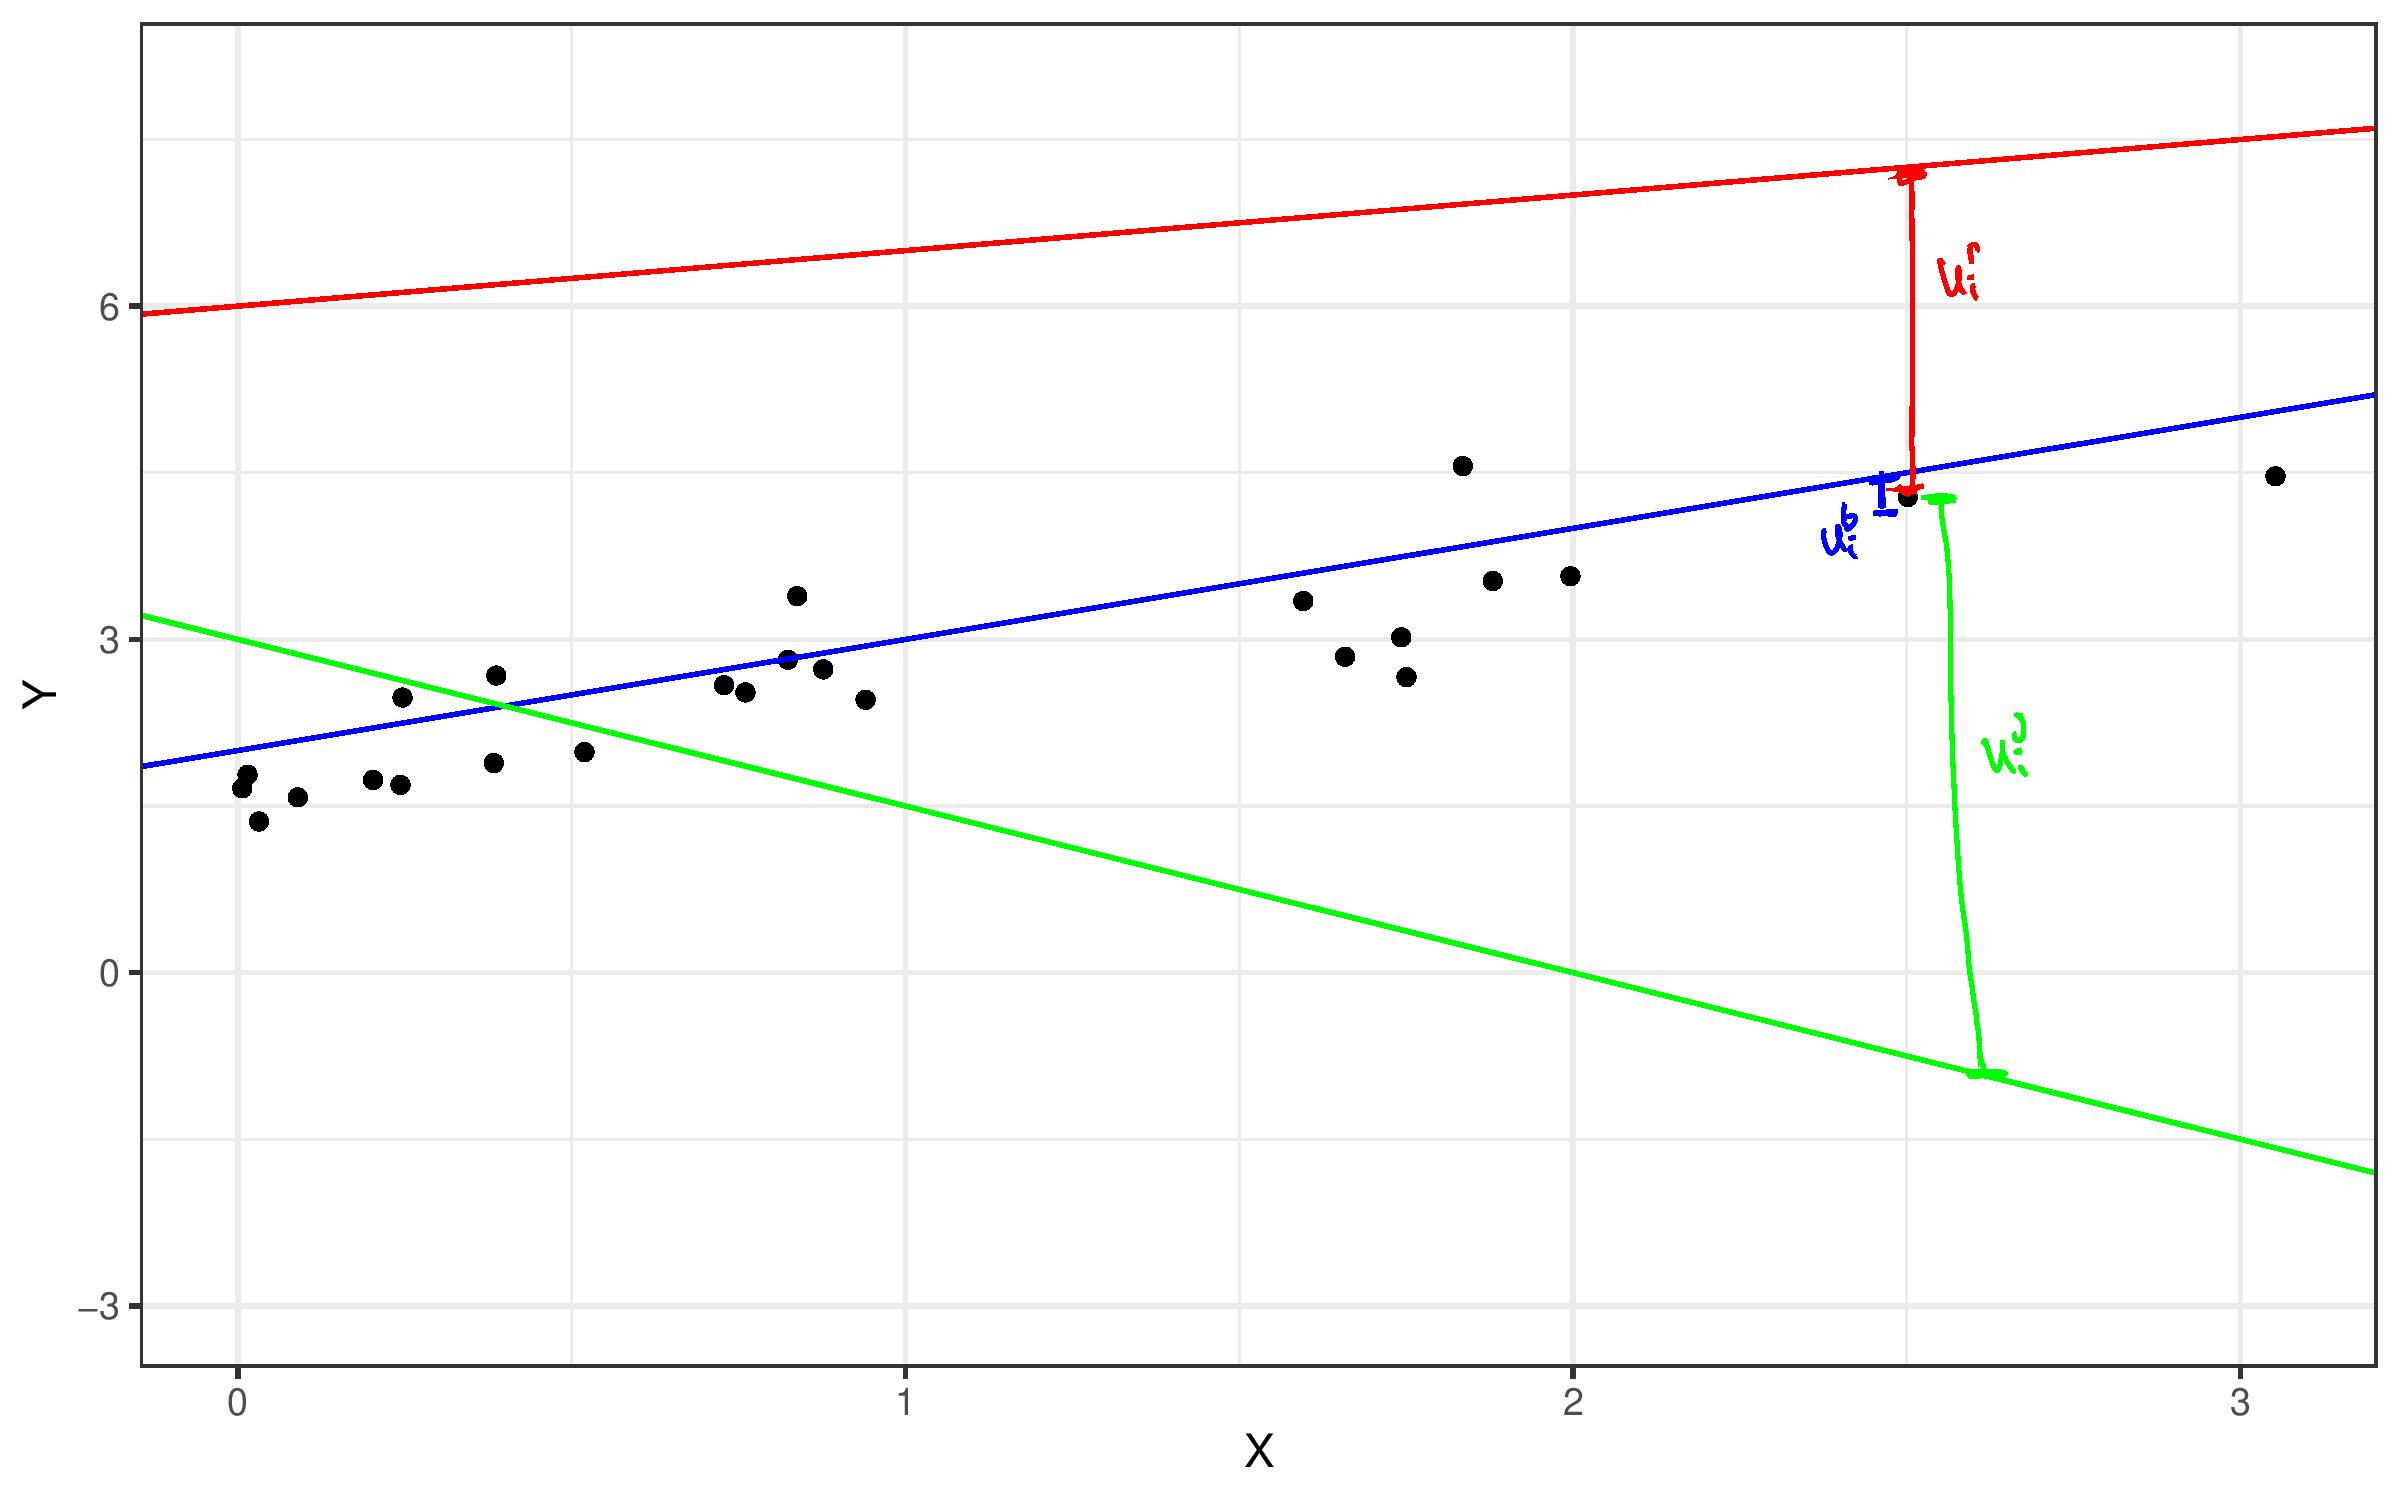
\includegraphics{ols_lines.jpg}

It's clear from the figure that the blue line ``fits better'' than the
green line or the red line. If you take a second and think about the
reason why this is the case, you will notice that the reason why you
know that it fits better is because the points \emph{tend to be closer}
to the blue line than to the red line or the green line.

In the figure, I drew three additional lines that are labeled \(U_i^b\),
\(U_i^g\), and \(U_i^r\) which are just the difference between the blue
line, the green line, and the red line and the corresponding data point
in the figure. That is,

\[
  \begin{aligned}
  U_i^b &= Y_i - b_0^b - b_1^b X_i \\
  U_i^g &= Y_i - b_0^g - b_1^g X_i \\
  U_i^r &= Y_i - b_0^r - b_1^r X_i
  \end{aligned}
\] where, for example, \(b_0^b\) and \(b_1^b\) are the intercept and
slope of the blue line, \(b_0^g\) and \(b_1^g\) are the intercept and
slope of the green line, etc. Clearly, the blue line fits this data
point than the others, but we need to deal with a couple of issues to
formalize this thinking. First, \(U_i^b\) and \(U_i^r\) are both less
than 0 (because both of those lines sit above the data point) indicating
that we can't just choose the line where \(U_i\) is the smallest --- for
this point, that strategy would result in us liking the red line the
most. Instead, we need a measure of distance that turns negative values
of \(U_i\) into positive values and is larger for big negative values of
\(U_i\) too. We'll use the same quadratic distance that we've used
before to deal with this issue; that is, we'll define the distance
between a line and the point as \({U_i^b}^2\) for the blue line,
\({U_i^g}^2\) and \({U_i^r}^2\) for the green and red lines.

Second, the above discussion computes the distance between the line and
the data for a single point. We want to extend this argument to all the
data points. And we can do that by computing the average distance
between the line and the points across all points. That is given by

\[
  \frac{1}{n}\sum_{i=1}^n {U_i^b}^2, \quad \frac{1}{n}\sum_{i=1}^n {U_i^g}^2, \quad \frac{1}{n}\sum_{i=1}^n {U_i^r}^2
\] for the blue line, green line, and red line. These are actually
numbers that we can compute.

\begin{Shaded}
\begin{Highlighting}[]
\CommentTok{\# intercept and slope of each line}
\CommentTok{\# (I just picked these)}
\NormalTok{int\_blue }\OtherTok{\textless{}{-}} \DecValTok{2}
\NormalTok{slope\_blue }\OtherTok{\textless{}{-}} \DecValTok{1}
\NormalTok{int\_green }\OtherTok{\textless{}{-}} \DecValTok{3}
\NormalTok{slope\_green }\OtherTok{\textless{}{-}} \SpecialCharTok{{-}}\FloatTok{1.5}
\NormalTok{int\_red }\OtherTok{\textless{}{-}} \DecValTok{6}
\NormalTok{slope\_red }\OtherTok{\textless{}{-}} \FloatTok{0.5}

\CommentTok{\# compute "errors"}
\NormalTok{Ub }\OtherTok{\textless{}{-}}\NormalTok{ Y }\SpecialCharTok{{-}}\NormalTok{ int\_blue }\SpecialCharTok{{-}}\NormalTok{ slope\_blue}\SpecialCharTok{*}\NormalTok{X}
\NormalTok{Ug }\OtherTok{\textless{}{-}}\NormalTok{ Y }\SpecialCharTok{{-}}\NormalTok{ int\_green }\SpecialCharTok{{-}}\NormalTok{ slope\_green}\SpecialCharTok{*}\NormalTok{X}
\NormalTok{Ur }\OtherTok{\textless{}{-}}\NormalTok{ Y }\SpecialCharTok{{-}}\NormalTok{ int\_red }\SpecialCharTok{{-}}\NormalTok{ slope\_red}\SpecialCharTok{*}\NormalTok{X}

\CommentTok{\# compute distances}
\NormalTok{dist\_blue }\OtherTok{\textless{}{-}} \FunctionTok{mean}\NormalTok{(Ub}\SpecialCharTok{\^{}}\DecValTok{2}\NormalTok{)}
\NormalTok{dist\_green }\OtherTok{\textless{}{-}} \FunctionTok{mean}\NormalTok{(Ug}\SpecialCharTok{\^{}}\DecValTok{2}\NormalTok{)}
\NormalTok{dist\_red }\OtherTok{\textless{}{-}} \FunctionTok{mean}\NormalTok{(Ur}\SpecialCharTok{\^{}}\DecValTok{2}\NormalTok{)}

\CommentTok{\# report distances}
\FunctionTok{round}\NormalTok{(}\FunctionTok{data.frame}\NormalTok{(dist\_blue, dist\_green, dist\_red), }\DecValTok{3}\NormalTok{)}
\end{Highlighting}
\end{Shaded}

\begin{verbatim}
  dist_blue dist_green dist_red
1     0.255      5.828   14.728
\end{verbatim}

This corroborates our earlier intuition --- the blue line appears to fit
the data much better than the other two lines.

It turns out that we can use the same sort of idea as above to choose
not just among three possible lines to fit the data, but to choose among
\emph{all possible lines}. More generally than we have been doing, let's
write

\[
  Y_i = b_0 + b_1 X_i + U_i(b_0,b_1)
\] In other words, for any values of \(b_0\) and \(b_1\) that we would
like to plug in (say like for the green line or red line in the figure
above), we can define \(U_i(b_0,b_1)\) to be whatever is leftover
between the line and the actual data.

We can choose the line (by choosing values of \(b_0\) and \(b_1\)) that
minimizes the average distance between the line and the points. In other
words, we will set

\[
  \begin{aligned}
  (\hat{\beta}_0, \hat{\beta}_1) &= \underset{b_0,b_1}{\textrm{argmin}} \frac{1}{n} \sum_{i=1}^n U_i(b_0,b_1)^2 \\
  &= \underset{b_0,b_1}{\textrm{argmin}} \frac{1}{n} \sum_{i=1}^n (Y_i - b_0 - b_1 X_i)^2
  \end{aligned}
\] This is a complicated looking mathematical expression, but I think
the intuition is pretty easy to understand. It says that we want to find
the values of \(b_0\) and \(b_1\) that make the distance between the
points and the line as small as possible on average. Whatever these
values are, that is what we are going to set \(\hat{\beta}_0\) and
\(\hat{\beta}_1\) --- our estimates of \(\beta_0\) and \(\beta_1\) ---
to be.

How can you do this? One idea is to do it numerically --- you could try
out a ton of different combinations of \(b_0\) and \(b_1\) and pick
which one fits the best. Your computer could probably actually do this,
but it would become quite a hard problem as we added more and more
regressors.

It turns out that we can actually find a solution for the values of
\(b_0\) and \(b_1\) that minimize the above expression using calculus.

You probably recall how to minimize a function. You take its derivative,
set it equal to 0, and solve that equation. {[}It's actually a little
more complicated than that because you need to ensure that you're
finding a minimum rather than a maximum, but the above equation is
actually quadratic, so it will have a minimum.{]}

That's all that we will do here --- just the thing we need to take the
derivative of looks complicated. Actually, the \(\frac{1}{n}\) and
\(\sum\) terms will just hang around. For the rest though, we need to
use the \emph{chain rule}; that is, we need to take the derivative of
the outside and then multiply by the derivative of the inside. We also
need to take the derivative both with respect to \(b_0\) and with
respect to \(b_1\).

Let's start by taking the derivative with respect to \(b_0\) and setting
it equal to 0.

\[
  -\frac{2}{n}\sum_{i=1}^n (Y_i - \hat{\beta}_0 - \hat{\beta}_1 X_i) = 0 (\#eq:foc-bet0)
\] where the \(2\) comes from taking the deriviative of the squared part
and the negative sign at the beginning comes from taking the derivative
of \(-b_0\) on the inside. I also replaced \(b_0\) and \(b_1\) here
since \(\hat{\beta}_0\) and \(\hat{\beta}_1\) are the values that will
solve this equation.

Next, let's take the derivative with respect to \(b_1\): \[
  -\frac{2}{n} \sum_{i=1}^n (Y_i - \hat{\beta}_0 - \hat{\beta}_1 X_i) X_i = 0 (\#eq:foc-bet1)
\]\\
where the 2 comes from taking the derivative of the squared part, and
the negative sign at the beginning and \(X_i\) at the end come from
taking the derivative of the inside with respect to \(b_1\).

All we have to do now is to solve these Equations @ref(eq:foc-bet0) and
@ref(eq:foc-bet1) for \(\hat{\beta}_0\) and \(\hat{\beta}_1\). Before we
do it, let me just mention that we are about to do some fairly
challenging algebra, but that is all it is. Conceptually, it is just the
same as solving a system of two equations with two unknowns that you
probably did at some point in high school.

Starting with the first equation,

\[
  \begin{aligned}
  & \phantom{\implies} -\frac{2}{n} \sum_{i=1}^n (Y_i - \hat{\beta}_0 - \hat{\beta}_1 X_i) &= 0 \\
  & \implies \frac{1}{n} \sum_{i=1}^n (Y_i - \hat{\beta}_0 - \hat{\beta}_1 X_i) &= 0 \\
  & \implies \bar{Y} - \hat{\beta}_0 - \hat{\beta}_1 \bar{X} &= 0 \\
  & \implies \boxed{\hat{\beta}_0 = \bar{Y} - \hat{\beta}_1 \bar{X}} 
  \end{aligned} 
\] where the second line holds by dividing both sides by \(-2\), the
third line holds by pushing the summation through the sums/differences
and simplifying terms, and the last line holds by rearranging to solve
for \(\hat{\beta}_0\).

Now, let's use the above result and Equation @ref(eq:foc-bet1) to solve
for \(\hat{\beta}_1\).

\[
  \begin{aligned}
  & \phantom{\implies} -\frac{2}{n} \sum_{i=1}^n (Y_i - \hat{\beta}_0 - \hat{\beta}_1) X_i &= 0 \\
  & \implies  \frac{1}{n} \sum_{i=1}^n (Y_i - \hat{\beta}_0 - \hat{\beta}_1) X_i) X_i &= 0 \\
  & \implies  \frac{1}{n} \sum_{i=1}^n (Y_i - (\bar{Y} - \hat{\beta}_1 \bar{X}) - \hat{\beta}_1 X_i) X_i &= 0 \\
  & \implies  \frac{1}{n} \sum_{i=1}^n X_i Y_i - \bar{Y} \frac{1}{n} \sum_{i=1}^n X_i + \hat{\beta}_1 \bar{X} \frac{1}{n} \sum_{i=1}^n X_i - \hat{\beta}_1 \frac{1}{n} \sum_{i=1}^n X_i^2 &= 0  \\
\end{aligned}
\] Let me explain each line and then we will keep going. The second line
holds because the \(-2\) can just be canceled on each side, the third
line holds by plugging in the expression we derived for
\(\hat{\beta}_0\) above, and the last line holds by splitting up the
summation and bringing out terms that do not change across \(i\). Let's
keep going

\[
\begin{aligned}
  \implies  \frac{1}{n} \sum_{i=1}^n X_i Y_i - \bar{X}\bar{Y} &= \hat{\beta}_1\left(\frac{1}{n} \sum_{i=1}^n X_i^2 - \bar{X}^2 \right) \\
  \implies  \hat{\beta}_1 &= \frac{\frac{1}{n} \sum_{i=1}^n X_i Y_i - \bar{X}\bar{Y}}{\frac{1}{n} \sum_{i=1}^n X_i^2 - \bar{X}^2} \\
  \implies  & \boxed{\hat{\beta}_1 = \frac{\widehat{\Cov}(X,Y)}{\widehat{\Var}(X)}}
  \end{aligned}
\] where the first line holds by using the definition of \(\bar{X}\) and
moving some terms to the other side. The second equality holds by
dividing both sides by
\(\left(\frac{1}{n} \displaystyle \sum_{i=1}^n X_i^2 - \bar{X}^2 \right)\),
and the last equality holds by the definition of sample covariance and
variance.

{Side-Comment:} I'd like to point out one more time that our estimates
\(\hat{\beta}_0\) and \(\hat{\beta}_1\) are generally not exactly equal
to \(\beta_0\) and \(\beta_1\). The figure earlier in this section was
generated using simulated data where I set \(\beta_0=2\) and
\(\beta_1=1\). However, we estimate \(\hat{\beta}_0 = 1.75\) and
\(\hat{\beta}_1 = 0.95\) using the simulated data in that figure. These
lines are close to each other, but not exactly the same.

Further, recall that we defined the \textbf{error term} \(U_i\) from

\[
  Y_i = \beta_0 + \beta_1 X_i + U_i
\] which is the difference between individual \(i\)'s outcome and the
\emph{population} regression line.

Similarly, we define the \textbf{residual} \(\hat{U}_i\) as

\[
  Y_i = \hat{\beta}_0 + \hat{\beta}_1 X_i + \hat{U}_i
\] so that \(\hat{U}_i\) is the difference between individual \(i\)'s
outcome and the estimated regression line. Moreover, since generally
\(\beta_0 \neq \hat{\beta}_0\) and \(\beta_1 \neq \hat{\beta}_1\),
generally \(U_i \neq \hat{U}_i\).

\subsection{Computation}\label{computation-7}

Before moving on, let's just confirm that the formulas that we derived
are actually what \texttt{R} uses in order to estimates the parameters
in a regression.

\begin{Shaded}
\begin{Highlighting}[]
\CommentTok{\# using lm}
\NormalTok{reg8 }\OtherTok{\textless{}{-}} \FunctionTok{lm}\NormalTok{(mpg }\SpecialCharTok{\textasciitilde{}}\NormalTok{ hp, }\AttributeTok{data=}\NormalTok{mtcars)}
\FunctionTok{summary}\NormalTok{(reg8)}
\end{Highlighting}
\end{Shaded}

\begin{verbatim}

Call:
lm(formula = mpg ~ hp, data = mtcars)

Residuals:
    Min      1Q  Median      3Q     Max 
-5.7121 -2.1122 -0.8854  1.5819  8.2360 

Coefficients:
            Estimate Std. Error t value Pr(>|t|)    
(Intercept) 30.09886    1.63392  18.421  < 2e-16 ***
hp          -0.06823    0.01012  -6.742 1.79e-07 ***
---
Signif. codes:  0 '***' 0.001 '**' 0.01 '*' 0.05 '.' 0.1 ' ' 1

Residual standard error: 3.863 on 30 degrees of freedom
Multiple R-squared:  0.6024,    Adjusted R-squared:  0.5892 
F-statistic: 45.46 on 1 and 30 DF,  p-value: 1.788e-07
\end{verbatim}

\begin{Shaded}
\begin{Highlighting}[]
\CommentTok{\# using our formulas}
\NormalTok{bet1 }\OtherTok{\textless{}{-}} \FunctionTok{cov}\NormalTok{(mtcars}\SpecialCharTok{$}\NormalTok{mpg, mtcars}\SpecialCharTok{$}\NormalTok{hp) }\SpecialCharTok{/} \FunctionTok{var}\NormalTok{(mtcars}\SpecialCharTok{$}\NormalTok{hp)}

\NormalTok{bet0 }\OtherTok{\textless{}{-}} \FunctionTok{mean}\NormalTok{(mtcars}\SpecialCharTok{$}\NormalTok{mpg) }\SpecialCharTok{{-}}\NormalTok{ bet1}\SpecialCharTok{*}\FunctionTok{mean}\NormalTok{(mtcars}\SpecialCharTok{$}\NormalTok{hp)}

\CommentTok{\# print results}
\FunctionTok{data.frame}\NormalTok{(}\AttributeTok{bet0=}\NormalTok{bet0, }\AttributeTok{bet1=}\NormalTok{bet1)}
\end{Highlighting}
\end{Shaded}

\begin{verbatim}
      bet0        bet1
1 30.09886 -0.06822828
\end{verbatim}

and they are identical.

\section{More than one regressor}\label{more-than-one-regressor}

Now, let's suppose that you want to estimate a more complicated
regressions like

\[
  Y = \beta_0 + \beta_1 X_1 + \beta_2 X_2 + \beta_3 X_3 + U
\]

or, even more generally,

\[
  Y = \beta_0 + \beta_1 X_1 + \cdots + \beta_k X_k + U
\] We can still choose the line that best fits the data by solving

\[
  (\hat{\beta}_0, \hat{\beta}_1, \ldots, \hat{\beta}_k) = \underset{b_0,b_1,\ldots,b_k}{\textrm{argmin}} \frac{1}{n} \sum_{i=1}^n (Y_i - b_0 - b_1 X_{1i} - \cdots - b_k X_{ki})^2
\] To do it, we would need to take the derivative with respect to
\(b_0, b_1, \ldots, b_k\). This will give a system of equations with
\((k+1)\) equations and \((k+1)\) unknowns. You can solve this --- it
actually is quite easy / very similar to what we just did if you know
just a little bit of linear algebra, but this is beyond the scope of our
course --- and it is quite easy for the computer to solve.

\bookmarksetup{startatroot}

\chapter{Inference}\label{inference-1}

\[
\newcommand{\E}{\mathbb{E}}
\renewcommand{\P}{\textrm{P}}
\let\L\relax
\newcommand{\L}{\textrm{L}} %doesn't work in .qmd, place this command at start of qmd file to use it
\newcommand{\F}{\textrm{F}}
\newcommand{\var}{\textrm{var}}
\newcommand{\cov}{\textrm{cov}}
\newcommand{\corr}{\textrm{corr}}
\newcommand{\Var}{\mathrm{Var}}
\newcommand{\Cov}{\mathrm{Cov}}
\newcommand{\Corr}{\mathrm{Corr}}
\newcommand{\sd}{\mathrm{sd}}
\newcommand{\se}{\mathrm{s.e.}}
\newcommand{\T}{T}
\newcommand{\indicator}[1]{\mathbb{1}\{#1\}}
\newcommand\independent{\perp \!\!\! \perp}
\newcommand{\N}{\mathcal{N}}
\]

\section{Inference}\label{inference-2}

SW 4.5, 5.1, 5.2, 6.6

We discussed in class the practical issues of inference in linear
regression models.

These results rely on arguments building on the Central Limit Theorem
(this should not surprise you as it is similar to the case for the
asymptotic distribution of \(\sqrt{n}(\bar{Y} - \E[Y]))\) that we
discussed earlier in the semester.

In this section, I sketch these types of arguments for you. This
material is advanced, but I suggest that you study this material.

We are going to show that, in the simple linear regression model,
\begin{align*}
  \sqrt{n}(\hat{\beta}_1 - \beta_1) \rightarrow N(0,V) \quad \textrm{as} \ n \rightarrow \infty
\end{align*} where \begin{align*}
  V = \frac{\E[(X-\E[X])^2 U^2]}{\var(X)^2}
\end{align*} and discuss how to use this result to conduct inference.

Let's start by showing why this result holds.

To start with, recall that \begin{align}
  \hat{\beta}_1 = \frac{\widehat{\cov}(X,Y)}{\widehat{\var}(X)} (\#eq:b1)
\end{align}

Before providing a main result, let's start with noting the following:

\emph{Helpful Intermediate Result 1} Notice that \begin{align*}
  \frac{1}{n}\sum_{i=1}^n \Big( (X_i - \bar{X})\bar{Y}\Big) &= \bar{Y} \frac{1}{n}\sum_{i=1}^n \Big( X_i-\bar{X} \Big) \\
  &= \bar{Y} \left( \frac{1}{n}\sum_{i=1}^n X_i - \frac{1}{n}\sum_{i=1}^n \bar{X} \right) \\
  &= \bar{Y} \Big(\bar{X} - \bar{X} \Big) \\
  &= 0
\end{align*} where the first equality just pulls \(\bar{Y}\) out of the
summation (it is a constant with respect to the summation), the second
equality pushes the summation through the difference, the first part of
the third equality holds by the definition of \(\bar{X}\) and the second
part holds because it is an average of a constant.

This implies that \begin{align}
  \frac{1}{n}\sum_{i=1}^n \Big( (X_i - \bar{X})(Y_i - \bar{Y})\Big) = \frac{1}{n}\sum_{i=1}^n \Big( (X_i - \bar{X})Y_i\Big) (\#eq:hr1)
\end{align} and very similar arguments (basically the same arguments in
reverse) also imply that \begin{align}
  \frac{1}{n}\sum_{i=1}^n \Big( (X_i - \bar{X})X_i\Big) = \frac{1}{n}\sum_{i=1}^n \Big( (X_i - \bar{X})(X_i - \bar{X})\Big) (\#eq:hr2)
\end{align} We use both @ref(eq:hr1) and @ref(eq:hr2) below.

\vspace{100pt}

Next, consider the numerator in @ref(eq:b1) \begin{align*}
  \widehat{\cov}(X,Y) &= \frac{1}{n} \sum_{i=1}^n (X_i - \bar{X})(Y_i - \bar{Y}) \\
  &= \frac{1}{n} \sum_{i=1}^n (X_i - \bar{X})Y_i \\
  &= \frac{1}{n} \sum_{i=1}^n (X_i - \bar{X})(\beta_0 + \beta_1 X_i + U_i) \\
  &= \underbrace{\beta_0 \frac{1}{n} \sum_{i=1}^n (X_i - \bar{X})}_{(A)} + \underbrace{\beta_1 \frac{1}{n} \sum_{i=1}^n (X_i - \bar{X}) X_i}_{(B)} + \underbrace{\frac{1}{n} \sum_{i=1}^n (X_i - \bar{X}) U_i}_{(C)}) \\
\end{align*} where the first equality holds by the definition of sample
covariance, the second equality holds by @ref(eq:hr1), the third
equality plugs in for \(Y_i\), and the last equality combines terms and
passes the summation through the additions/subtractions.

Now, let's consider each of these in turn.

For (A), \begin{align*}
  \frac{1}{n} \sum_{i=1}^n X_i = \bar{X} \qquad \textrm{and} \qquad \frac{1}{n} \sum_{i=1}^n \bar{X} = \bar{X}
\end{align*} which implies that this term is equal to 0.

For (B), notice that \begin{align*}
  \beta_1 \frac{1}{n} \sum_{i=1}^n (X_i - \bar{X}) X_i &= \beta_1 \frac{1}{n} \sum_{i=1}^n (X_i - \bar{X}) (X_i - \bar{X}) \\
  &= \beta_1 \widehat{\var}(X)
\end{align*} where the first equality holds by @ref(eq:hr2) and the
second equality holds by the definition of sample variance.

For (C), well, we'll just carry that one around for now.

Plugging in the expressions for (A), (B), and (C) back into Equation
@ref(eq:b1) implies that \begin{align*}
  \hat{\beta}_1 = \beta_1 + \frac{1}{n} \sum_{i=1}^n \frac{(X_i - \bar{X}) U_i}{\widehat{\var}(X)}
\end{align*} Next, re-arranging terms and multiplying both sides by
\(\sqrt{n}\) implies that \begin{align*}
  \sqrt{n}(\hat{\beta}_1 - \beta_1) &= \sqrt{n} \left(\frac{1}{n} \sum_{i=1}^n \frac{(X_i - \bar{X}) U_i}{\widehat{\var}(X)}\right) \\
  & \approx \sqrt{n} \left(\frac{1}{n} \sum_{i=1}^n \frac{(X_i - \E[X]) U_i}{\var(X)}\right)
\end{align*} The last line (the approximately one) is kind of a weak
argument, but basically you can replace \(\bar{X}\) and
\(\widehat{\var}(X)\) and the effect of this replacement will converge
to 0 in large samples (this is the reason for the approximately) --- if
you want a more complete explanation, sign up for my graduate
econometrics class next semester.

Is this helpful? It may not be obvious, but the right hand side of the
above equation is actually something that we can apply the Central Limit
Theorem to. In particular, maybe it is helpful to define
\(Z_i = \frac{(X_i - \E[X]) U_i}{\var(X)}\). We know that we could apply
a Central Limit Theorem to
\(\sqrt{n}\left( \frac{1}{n} \sum_{i=1}^n Z_i \right)\) if (i) \(Z_i\)
had mean 0, and (ii) it is iid. That it is iid holds immediately from
the random sampling assumption. For mean 0, \begin{align*}
  \E[Z] &= \E\left[ \frac{(X - \E[X]) U}{\var(X)}\right] \\
  &= \frac{1}{\var(X)} \E[(X - \E[X]) U] \\
  &= \frac{1}{\var(X)} \E[(X - \E[X]) \underbrace{\E[U|X]}_{=0}] \\
  &= 0
\end{align*} where the only challenging line here is the third one holds
from the Law of Iterated Expectations. This means that we can apply the
central limit theorem, and in particular,
\(\sqrt{n} \left( \frac{1}{n} \sum_{i=1}^n Z_i \right) \rightarrow N(0,V)\)
where \(V=\var(Z) = \E[Z^2]\) (where the 2nd equality here holds because
\(Z\) has mean 0). Now, just substituting back in for \(Z\) implies that
\begin{align*}
  \sqrt{n}(\hat{\beta}_1 - \beta_1) \rightarrow N(0,V)
\end{align*} where \begin{align}
  V &= \E\left[ \left( \frac{(X - \E[X]) U}{\var(X)} \right)^2 \right] \nonumber \\
  &= \E\left[ \frac{(X - \E[X])^2 U^2}{\var(X)^2}\right] (\#eq:V)
\end{align} which is what we were aiming for.

Given this result, all our previous work on standard errors,
t-statistics, p-values, and confidence intervals applies. First, let me
mention the way that you would estimate \(V\) (same as always, just
replace the population quantities with corresponding sample quantities).

\[
  \hat{V} = \frac{ \frac{1}{n} \displaystyle \sum_{i=1}^n (X_i - \bar{X})^2 \hat{U}_i^2}{\widehat{\Var}(X)^2}
\]

where \(\hat{U}_i\) are the residuals.

Now, standard errors are just the same as before (the only difference is
that \(\hat{V}\) itself has changed)

\[
\begin{aligned}
  \textrm{s.e.}(\hat{\beta}) &= \frac{\sqrt{\hat{V}}}{\sqrt{n}}
\end{aligned}
\]

By far the most common null hypothesis is \(H_0: \beta = 0\), which
suggests the following t-statistic:

\[
  t = \frac{\hat{\beta}}{\textrm{s.e.}(\hat{\beta})}
\] One can continue to calculate a p-value by

\[
  \textrm{p-value} = 2 \Phi(-|t|)
\] and a 95\% confidence interval is given by

\[
  CI = [\hat{\beta} - 1.96 \textrm{s.e.}(\hat{\beta}), \hat{\beta} + 1.96 \textrm{s.e.}(\hat{\beta})]
\]

\subsection{Computation}\label{computation-8}

Let's check if what we derived is what we can compute using \texttt{R}.

\begin{Shaded}
\begin{Highlighting}[]
\CommentTok{\# this is the same regression as in the previous section}
\FunctionTok{summary}\NormalTok{(reg8)}
\end{Highlighting}
\end{Shaded}

\begin{verbatim}

Call:
lm(formula = mpg ~ hp, data = mtcars)

Residuals:
    Min      1Q  Median      3Q     Max 
-5.7121 -2.1122 -0.8854  1.5819  8.2360 

Coefficients:
            Estimate Std. Error t value Pr(>|t|)    
(Intercept) 30.09886    1.63392  18.421  < 2e-16 ***
hp          -0.06823    0.01012  -6.742 1.79e-07 ***
---
Signif. codes:  0 '***' 0.001 '**' 0.01 '*' 0.05 '.' 0.1 ' ' 1

Residual standard error: 3.863 on 30 degrees of freedom
Multiple R-squared:  0.6024,    Adjusted R-squared:  0.5892 
F-statistic: 45.46 on 1 and 30 DF,  p-value: 1.788e-07
\end{verbatim}

\begin{Shaded}
\begin{Highlighting}[]
\CommentTok{\# show previous calcuations}
\FunctionTok{data.frame}\NormalTok{(}\AttributeTok{bet0=}\NormalTok{bet0, }\AttributeTok{bet1=}\NormalTok{bet1)}
\end{Highlighting}
\end{Shaded}

\begin{verbatim}
      bet0        bet1
1 30.09886 -0.06822828
\end{verbatim}

\begin{Shaded}
\begin{Highlighting}[]
\CommentTok{\# components of Vhat}
\NormalTok{Y }\OtherTok{\textless{}{-}}\NormalTok{ mtcars}\SpecialCharTok{$}\NormalTok{mpg}
\NormalTok{X }\OtherTok{\textless{}{-}}\NormalTok{ mtcars}\SpecialCharTok{$}\NormalTok{hp}
\NormalTok{Uhat }\OtherTok{\textless{}{-}}\NormalTok{ Y }\SpecialCharTok{{-}}\NormalTok{ bet0 }\SpecialCharTok{{-}}\NormalTok{ bet1}\SpecialCharTok{*}\NormalTok{X}
\NormalTok{Xbar }\OtherTok{\textless{}{-}} \FunctionTok{mean}\NormalTok{(X)}
\NormalTok{varX }\OtherTok{\textless{}{-}} \FunctionTok{mean}\NormalTok{( (X}\SpecialCharTok{{-}}\NormalTok{Xbar)}\SpecialCharTok{\^{}}\DecValTok{2}\NormalTok{ )}
\NormalTok{Vhat }\OtherTok{\textless{}{-}} \FunctionTok{mean}\NormalTok{( (X}\SpecialCharTok{{-}}\NormalTok{Xbar)}\SpecialCharTok{\^{}}\DecValTok{2} \SpecialCharTok{*}\NormalTok{ Uhat}\SpecialCharTok{\^{}}\DecValTok{2}\NormalTok{ ) }\SpecialCharTok{/}\NormalTok{ ( varX}\SpecialCharTok{\^{}}\DecValTok{2}\NormalTok{ )}
\NormalTok{n }\OtherTok{\textless{}{-}} \FunctionTok{nrow}\NormalTok{(mtcars)}
\NormalTok{se }\OtherTok{\textless{}{-}} \FunctionTok{sqrt}\NormalTok{(Vhat)}\SpecialCharTok{/}\FunctionTok{sqrt}\NormalTok{(n)}
\NormalTok{t\_stat }\OtherTok{\textless{}{-}}\NormalTok{ bet1}\SpecialCharTok{/}\NormalTok{se}
\NormalTok{p\_val }\OtherTok{\textless{}{-}} \DecValTok{2}\SpecialCharTok{*}\FunctionTok{pnorm}\NormalTok{(}\SpecialCharTok{{-}}\FunctionTok{abs}\NormalTok{(t\_stat))}
\NormalTok{ci\_L }\OtherTok{\textless{}{-}}\NormalTok{ bet1 }\SpecialCharTok{{-}} \FloatTok{1.96}\SpecialCharTok{*}\NormalTok{se}
\NormalTok{ci\_U }\OtherTok{\textless{}{-}}\NormalTok{ bet1 }\SpecialCharTok{+} \FloatTok{1.96}\SpecialCharTok{*}\NormalTok{se}

\CommentTok{\# print results}
\FunctionTok{round}\NormalTok{(}\FunctionTok{data.frame}\NormalTok{(se, t\_stat, p\_val, ci\_L, ci\_U),}\DecValTok{5}\NormalTok{)}
\end{Highlighting}
\end{Shaded}

\begin{verbatim}
       se   t_stat p_val     ci_L     ci_U
1 0.01313 -5.19644     0 -0.09396 -0.04249
\end{verbatim}

Interestingly, these are not \emph{exactly} the same as what comes from
the \texttt{lm} command. Here's what the difference is: \texttt{R} makes
a simplifying assumption called ``homoskedasticity'' that simplifies the
expression for the variance. This can result in slightly different
standard errors (and therefore slightly different t-statistics,
p-values, and confidence intervals too) than the ones we calculated.

An alternative package that is popular among economists for estimating
regressions and getting ``heteroskedasticity robust'' standard errors is
the \texttt{estimatr} package.

\begin{Shaded}
\begin{Highlighting}[]
\FunctionTok{library}\NormalTok{(estimatr)}

\NormalTok{reg9 }\OtherTok{\textless{}{-}} \FunctionTok{lm\_robust}\NormalTok{(mpg }\SpecialCharTok{\textasciitilde{}}\NormalTok{ hp, }\AttributeTok{data=}\NormalTok{mtcars, }\AttributeTok{se\_type=}\StringTok{"HC0"}\NormalTok{)}
\FunctionTok{summary}\NormalTok{(reg9)}
\end{Highlighting}
\end{Shaded}

\begin{verbatim}

Call:
lm_robust(formula = mpg ~ hp, data = mtcars, se_type = "HC0")

Standard error type:  HC0 

Coefficients:
            Estimate Std. Error t value  Pr(>|t|) CI Lower CI Upper DF
(Intercept) 30.09886    2.01067  14.970 1.851e-15 25.99252 34.20520 30
hp          -0.06823    0.01313  -5.196 1.338e-05 -0.09504 -0.04141 30

Multiple R-squared:  0.6024 ,   Adjusted R-squared:  0.5892 
F-statistic:    27 on 1 and 30 DF,  p-value: 1.338e-05
\end{verbatim}

The ``HC0'' standard errors are ``heteroskedasticity consistent''
standard errors, and you can see that they match what we calculated
above.

\section{Lab 4: Birthweight and
Smoking}\label{lab-4-birthweight-and-smoking}

For this lab, we'll use the data \texttt{Birthweight\_Smoking} and study
the relationship between infant birthweight and mother's smoking
behavior.

\begin{enumerate}
\def\labelenumi{\arabic{enumi}.}
\item
  Run a regression of \(birthweight\) on \(smoker\). How do you
  interpret the results?
\item
  Use the \texttt{datasummary\_balance} function from the
  \texttt{modelsummary} package to provide summary statistics for each
  variable in the data separately by smoking status of the mother. Do
  you notice any interesting patterns?
\item
  Now run a regression of \(birthweight\) on \(smoker\), \(educ\),
  \(nprevisit\), \(age\), and \(alcohol\). How do you interpret the
  coefficient on \(smoker\)? How does its magnitude compare to the
  result from \#1? What do you make of this?
\item
  Now run a regression of \(birthweight\) on \(smoker\), the interaction
  of \(smoker\) and \(age\) and the other covariates (including \(age\))
  from \#3. How do you interpret the coefficient on \(smoker\) and the
  coefficient on the interaction term?
\item
  Now run a regression of \(birthweight\) on \(smoker\), the interaction
  of \(smoker\) and \(alcohol\) and the other covariates from \#3. How
  do you interpret the coefficient on \(smoker\) and the coefficient on
  the interaction term?
\item
  Now run a regression of \(birthweight\) on \(age\) and \(age^2\). Plot
  the predicted value of birthweight as a function of age for ages from
  18 to 44. What do you make of this?
\item
  Now run a regression of \(\log(birthweight)\) on \(smoker\) and the
  other covariates from \#3. How do you interpret the coefficient on
  \(smoker\)?
\end{enumerate}

\section{Lab 4: Solutions}\label{lab-4-solutions}

\begin{Shaded}
\begin{Highlighting}[]
\CommentTok{\# load packages}
\FunctionTok{library}\NormalTok{(haven)}
\FunctionTok{library}\NormalTok{(modelsummary)}
\FunctionTok{library}\NormalTok{(dplyr)}
\FunctionTok{library}\NormalTok{(ggplot2)}

\CommentTok{\# load data}
\NormalTok{Birthweight\_Smoking }\OtherTok{\textless{}{-}} \FunctionTok{read\_dta}\NormalTok{(}\StringTok{"data/birthweight\_smoking.dta"}\NormalTok{)}
\end{Highlighting}
\end{Shaded}

\begin{enumerate}
\def\labelenumi{\arabic{enumi}.}
\tightlist
\item
\end{enumerate}

\begin{Shaded}
\begin{Highlighting}[]
\NormalTok{reg1 }\OtherTok{\textless{}{-}} \FunctionTok{lm}\NormalTok{(birthweight }\SpecialCharTok{\textasciitilde{}}\NormalTok{ smoker, }\AttributeTok{data=}\NormalTok{Birthweight\_Smoking)}
\FunctionTok{summary}\NormalTok{(reg1)}
\end{Highlighting}
\end{Shaded}

\begin{verbatim}

Call:
lm(formula = birthweight ~ smoker, data = Birthweight_Smoking)

Residuals:
     Min       1Q   Median       3Q      Max 
-3007.06  -313.06    26.94   366.94  2322.94 

Coefficients:
            Estimate Std. Error t value Pr(>|t|)    
(Intercept)  3432.06      11.87 289.115   <2e-16 ***
smoker       -253.23      26.95  -9.396   <2e-16 ***
---
Signif. codes:  0 '***' 0.001 '**' 0.01 '*' 0.05 '.' 0.1 ' ' 1

Residual standard error: 583.7 on 2998 degrees of freedom
Multiple R-squared:  0.0286,    Adjusted R-squared:  0.02828 
F-statistic: 88.28 on 1 and 2998 DF,  p-value: < 2.2e-16
\end{verbatim}

We estimate that, on average, smoking reduces an infant's birthweight by
about 250 grams. The estimated effect is strongly statistically
significant, and (I am not an expert but) that seems like a large effect
of smoking to me.

\begin{enumerate}
\def\labelenumi{\arabic{enumi}.}
\setcounter{enumi}{1}
\tightlist
\item
\end{enumerate}

\begin{Shaded}
\begin{Highlighting}[]
\CommentTok{\# create smoker factor {-}{-}{-} just to make table look nicer}
\NormalTok{Birthweight\_Smoking}\SpecialCharTok{$}\NormalTok{smoker\_factor }\OtherTok{\textless{}{-}} \FunctionTok{as.factor}\NormalTok{(}\FunctionTok{ifelse}\NormalTok{(Birthweight\_Smoking}\SpecialCharTok{$}\NormalTok{smoker}\SpecialCharTok{==}\DecValTok{1}\NormalTok{, }\StringTok{"smoker"}\NormalTok{, }\StringTok{"non{-}smoker"}\NormalTok{))}
\FunctionTok{datasummary\_balance}\NormalTok{(}\SpecialCharTok{\textasciitilde{}}\NormalTok{smoker\_factor, }
                    \AttributeTok{data=}\NormalTok{dplyr}\SpecialCharTok{::}\FunctionTok{select}\NormalTok{(Birthweight\_Smoking, }\SpecialCharTok{{-}}\NormalTok{smoker),}
                    \AttributeTok{fmt=}\DecValTok{2}\NormalTok{)}
\end{Highlighting}
\end{Shaded}

\begin{table}
\centering
\begin{tblr}[         %% tabularray outer open
]                     %% tabularray outer close
{                     %% tabularray inner open
colspec={Q[]Q[]Q[]Q[]Q[]Q[]Q[]},
cell{1}{2}={c=2,}{halign=c,},
cell{1}{4}={c=2,}{halign=c,},
column{1}={halign=l,},
column{2}={halign=r,},
column{3}={halign=r,},
column{4}={halign=r,},
column{5}={halign=r,},
column{6}={halign=r,},
column{7}={halign=r,},
row{1}={halign=c,},
}                     %% tabularray inner close
\toprule
& non-smoker (N=2418) &  & smoker (N=582) &  &  &  \\ \cmidrule[lr]{2-3}\cmidrule[lr]{4-5}
& Mean & Std. Dev. & Mean & Std. Dev. & Diff. in Means & Std. Error \\ \midrule %% TinyTableHeader
nprevist    & \num{11.19}   & \num{3.50}   & \num{10.18}   & \num{4.23}   & \num{-1.01}   & \num{0.19}  \\
alcohol     & \num{0.01}    & \num{0.11}   & \num{0.05}    & \num{0.22}   & \num{0.04}    & \num{0.01}  \\
tripre1     & \num{0.83}    & \num{0.38}   & \num{0.70}    & \num{0.46}   & \num{-0.13}   & \num{0.02}  \\
tripre2     & \num{0.14}    & \num{0.34}   & \num{0.22}    & \num{0.41}   & \num{0.08}    & \num{0.02}  \\
tripre3     & \num{0.03}    & \num{0.16}   & \num{0.06}    & \num{0.24}   & \num{0.04}    & \num{0.01}  \\
tripre0     & \num{0.01}    & \num{0.08}   & \num{0.02}    & \num{0.15}   & \num{0.02}    & \num{0.01}  \\
birthweight & \num{3432.06} & \num{584.62} & \num{3178.83} & \num{580.01} & \num{-253.23} & \num{26.82} \\
unmarried   & \num{0.18}    & \num{0.38}   & \num{0.43}    & \num{0.50}   & \num{0.25}    & \num{0.02}  \\
educ        & \num{13.15}   & \num{2.21}   & \num{11.88}   & \num{1.62}   & \num{-1.27}   & \num{0.08}  \\
age         & \num{27.27}   & \num{5.37}   & \num{25.32}   & \num{5.06}   & \num{-1.95}   & \num{0.24}  \\
drinks      & \num{0.03}    & \num{0.47}   & \num{0.19}    & \num{1.23}   & \num{0.16}    & \num{0.05}  \\
\bottomrule
\end{tblr}
\end{table}

The things that stand out to me are:

\begin{itemize}
\item
  Birthweight tends to be notably lower for smokers relative to
  non-smokers. The difference is about 7.4\% lower birthweight for
  babies whose mothers smoked.
\item
  That said, smoking is also correlated with a number of other things
  that could be related to lower birthweights. Mothers who smoke went to
  fewer pre-natal visits on average, were more likely to be unmarried,
  were more likely to have drink alcohol during their pregnancy, were
  more likely to be less educated. They also were, on average, somewhat
  younger than mothers who did not smoke.
\end{itemize}

\begin{enumerate}
\def\labelenumi{\arabic{enumi}.}
\setcounter{enumi}{2}
\tightlist
\item
\end{enumerate}

\begin{Shaded}
\begin{Highlighting}[]
\NormalTok{reg3 }\OtherTok{\textless{}{-}} \FunctionTok{lm}\NormalTok{(birthweight }\SpecialCharTok{\textasciitilde{}}\NormalTok{ smoker }\SpecialCharTok{+}\NormalTok{ educ }\SpecialCharTok{+}\NormalTok{ nprevist }\SpecialCharTok{+}\NormalTok{ age }\SpecialCharTok{+}\NormalTok{ alcohol,}
           \AttributeTok{data=}\NormalTok{Birthweight\_Smoking)}
\FunctionTok{summary}\NormalTok{(reg3)}
\end{Highlighting}
\end{Shaded}

\begin{verbatim}

Call:
lm(formula = birthweight ~ smoker + educ + nprevist + age + alcohol, 
    data = Birthweight_Smoking)

Residuals:
     Min       1Q   Median       3Q      Max 
-2728.91  -305.26    24.69   359.63  2220.42 

Coefficients:
            Estimate Std. Error t value Pr(>|t|)    
(Intercept) 2924.963     74.185  39.428  < 2e-16 ***
smoker      -206.507     27.367  -7.546 5.93e-14 ***
educ           5.644      5.532   1.020    0.308    
nprevist      32.979      2.914  11.318  < 2e-16 ***
age            2.360      2.178   1.083    0.279    
alcohol      -39.512     76.365  -0.517    0.605    
---
Signif. codes:  0 '***' 0.001 '**' 0.01 '*' 0.05 '.' 0.1 ' ' 1

Residual standard error: 570.3 on 2994 degrees of freedom
Multiple R-squared:  0.07402,   Adjusted R-squared:  0.07247 
F-statistic: 47.86 on 5 and 2994 DF,  p-value: < 2.2e-16
\end{verbatim}

Here we estimate that smoking reduces an infant's birthweight by about
200 grams on average holding education, number of pre-natal visits, age,
and whether or not the mother consumed alcohol constant. The magnitude
of the estimated effect is somewhat smaller than the previous estimate.
Due to the discussion in \#2 (particularly, that smoking was correlated
with a number of other characteristics that are likely associated with
lower birthweights), this decrease in the magnitude is not surprising.

\begin{enumerate}
\def\labelenumi{\arabic{enumi}.}
\setcounter{enumi}{3}
\tightlist
\item
\end{enumerate}

\begin{Shaded}
\begin{Highlighting}[]
\NormalTok{reg4 }\OtherTok{\textless{}{-}} \FunctionTok{lm}\NormalTok{(birthweight }\SpecialCharTok{\textasciitilde{}}\NormalTok{ smoker }\SpecialCharTok{+} \FunctionTok{I}\NormalTok{(smoker}\SpecialCharTok{*}\NormalTok{age) }\SpecialCharTok{+}\NormalTok{ educ }\SpecialCharTok{+}\NormalTok{ nprevist }\SpecialCharTok{+}\NormalTok{ age }\SpecialCharTok{+}\NormalTok{ alcohol,}
           \AttributeTok{data=}\NormalTok{Birthweight\_Smoking)}
\FunctionTok{summary}\NormalTok{(reg4)}
\end{Highlighting}
\end{Shaded}

\begin{verbatim}

Call:
lm(formula = birthweight ~ smoker + I(smoker * age) + educ + 
    nprevist + age + alcohol, data = Birthweight_Smoking)

Residuals:
     Min       1Q   Median       3Q      Max 
-2722.56  -305.12    23.93   363.43  2244.67 

Coefficients:
                Estimate Std. Error t value Pr(>|t|)    
(Intercept)     2853.819     77.104  37.013  < 2e-16 ***
smoker           231.578    134.854   1.717 0.086036 .  
I(smoker * age)  -17.145      5.168  -3.317 0.000919 ***
educ               4.895      5.528   0.885 0.375968    
nprevist          32.482      2.913  11.151  < 2e-16 ***
age                5.528      2.375   2.328 0.019999 *  
alcohol          -22.556     76.409  -0.295 0.767864    
---
Signif. codes:  0 '***' 0.001 '**' 0.01 '*' 0.05 '.' 0.1 ' ' 1

Residual standard error: 569.4 on 2993 degrees of freedom
Multiple R-squared:  0.07741,   Adjusted R-squared:  0.07556 
F-statistic: 41.85 on 6 and 2993 DF,  p-value: < 2.2e-16
\end{verbatim}

We should be careful about the interpretatio here. We have estimated a
model like

\[
  \E[Birthweight|Smoker, Age, X] = \beta_0 + \beta_1 Smoker + \beta_2 Smoker \cdot Age + \cdots
\] Therefore, the partial effect of smoking is given by

\[
  \E[Birthweight | Smoker=1, Age, X] - \E[Birthweight | Smoker=0, Age, X] = \beta_1 + \beta_2 Age
\] Therefore, the partial effect of smoking depends on \(Age\). For
example, for \(Age=18\), the partial effect is
\(\beta_1 + \beta_2 (18)\). For \(Age=25\), the partial effect is
\(\beta_1 + \beta_2 (25)\), and for \(Age=35\), the partial effect is
\(\beta_1 + \beta_2 (35)\). Let's calculate the partial effect at each
of those ages.

\begin{Shaded}
\begin{Highlighting}[]
\NormalTok{bet1 }\OtherTok{\textless{}{-}} \FunctionTok{coef}\NormalTok{(reg4)[}\DecValTok{2}\NormalTok{]}
\NormalTok{bet2 }\OtherTok{\textless{}{-}} \FunctionTok{coef}\NormalTok{(reg4)[}\DecValTok{3}\NormalTok{]}

\NormalTok{pe\_18 }\OtherTok{\textless{}{-}}\NormalTok{ bet1 }\SpecialCharTok{+}\NormalTok{ bet2}\SpecialCharTok{*}\DecValTok{18}
\NormalTok{pe\_25 }\OtherTok{\textless{}{-}}\NormalTok{ bet1 }\SpecialCharTok{+}\NormalTok{ bet2}\SpecialCharTok{*}\DecValTok{25}
\NormalTok{pe\_35 }\OtherTok{\textless{}{-}}\NormalTok{ bet1 }\SpecialCharTok{+}\NormalTok{ bet2}\SpecialCharTok{*}\DecValTok{35}

\FunctionTok{round}\NormalTok{(}\FunctionTok{cbind.data.frame}\NormalTok{(pe\_18, pe\_25, pe\_35),}\DecValTok{2}\NormalTok{)}
\end{Highlighting}
\end{Shaded}

\begin{verbatim}
        pe_18   pe_25   pe_35
smoker -77.04 -197.05 -368.51
\end{verbatim}

This suggests substantially larger effects of smoking on birthweight for
older mothers.

\begin{Shaded}
\begin{Highlighting}[]
\NormalTok{reg5 }\OtherTok{\textless{}{-}} \FunctionTok{lm}\NormalTok{(birthweight }\SpecialCharTok{\textasciitilde{}}\NormalTok{ smoker }\SpecialCharTok{+} \FunctionTok{I}\NormalTok{(smoker}\SpecialCharTok{*}\NormalTok{alcohol) }\SpecialCharTok{+}\NormalTok{ educ }\SpecialCharTok{+}\NormalTok{ nprevist }\SpecialCharTok{+}\NormalTok{ age }\SpecialCharTok{+}\NormalTok{ alcohol,}
           \AttributeTok{data=}\NormalTok{Birthweight\_Smoking)}
\FunctionTok{summary}\NormalTok{(reg5)}
\end{Highlighting}
\end{Shaded}

\begin{verbatim}

Call:
lm(formula = birthweight ~ smoker + I(smoker * alcohol) + educ + 
    nprevist + age + alcohol, data = Birthweight_Smoking)

Residuals:
     Min       1Q   Median       3Q      Max 
-2728.99  -304.16    24.54   359.92  2222.10 

Coefficients:
                    Estimate Std. Error t value Pr(>|t|)    
(Intercept)         2924.844     74.185  39.426  < 2e-16 ***
smoker              -201.852     27.765  -7.270 4.57e-13 ***
I(smoker * alcohol) -151.860    152.717  -0.994    0.320    
educ                   5.612      5.532   1.014    0.310    
nprevist              32.844      2.917  11.260  < 2e-16 ***
age                    2.403      2.178   1.103    0.270    
alcohol               39.824    110.440   0.361    0.718    
---
Signif. codes:  0 '***' 0.001 '**' 0.01 '*' 0.05 '.' 0.1 ' ' 1

Residual standard error: 570.3 on 2993 degrees of freedom
Multiple R-squared:  0.07432,   Adjusted R-squared:  0.07247 
F-statistic: 40.05 on 6 and 2993 DF,  p-value: < 2.2e-16
\end{verbatim}

The point estimate suggests that the effect of smoking is larger for
women who consume alcohol and smoke than for women who do not drink
alcohol. This seems plausible, but our evidence is not very strong here
--- the estimates are not statistically significant at any conventional
significance level (the p-value is equal to 0.32).

\begin{enumerate}
\def\labelenumi{\arabic{enumi}.}
\setcounter{enumi}{5}
\tightlist
\item
\end{enumerate}

\begin{Shaded}
\begin{Highlighting}[]
\NormalTok{reg6 }\OtherTok{\textless{}{-}} \FunctionTok{lm}\NormalTok{(birthweight }\SpecialCharTok{\textasciitilde{}}\NormalTok{ age }\SpecialCharTok{+} \FunctionTok{I}\NormalTok{(age}\SpecialCharTok{\^{}}\DecValTok{2}\NormalTok{), }\AttributeTok{data=}\NormalTok{Birthweight\_Smoking)}
\FunctionTok{summary}\NormalTok{(reg6)}
\end{Highlighting}
\end{Shaded}

\begin{verbatim}

Call:
lm(formula = birthweight ~ age + I(age^2), data = Birthweight_Smoking)

Residuals:
     Min       1Q   Median       3Q      Max 
-2949.81  -312.81    30.43   371.03  2452.72 

Coefficients:
             Estimate Std. Error t value Pr(>|t|)    
(Intercept) 2502.8949   225.6016  11.094  < 2e-16 ***
age           58.1670    16.9212   3.438 0.000595 ***
I(age^2)      -0.9099     0.3099  -2.936 0.003353 ** 
---
Signif. codes:  0 '***' 0.001 '**' 0.01 '*' 0.05 '.' 0.1 ' ' 1

Residual standard error: 589.6 on 2997 degrees of freedom
Multiple R-squared:  0.009261,  Adjusted R-squared:  0.0086 
F-statistic: 14.01 on 2 and 2997 DF,  p-value: 8.813e-07
\end{verbatim}

\begin{Shaded}
\begin{Highlighting}[]
\NormalTok{preds }\OtherTok{\textless{}{-}} \FunctionTok{predict}\NormalTok{(reg6, }\AttributeTok{newdata=}\FunctionTok{data.frame}\NormalTok{(}\AttributeTok{age=}\FunctionTok{seq}\NormalTok{(}\DecValTok{18}\NormalTok{,}\DecValTok{40}\NormalTok{)))}
\FunctionTok{ggplot}\NormalTok{(}\FunctionTok{data.frame}\NormalTok{(}\AttributeTok{preds=}\NormalTok{preds, }\AttributeTok{age=}\FunctionTok{seq}\NormalTok{(}\DecValTok{18}\NormalTok{,}\DecValTok{40}\NormalTok{)), }\FunctionTok{aes}\NormalTok{(}\AttributeTok{x=}\NormalTok{age, }\AttributeTok{y=}\NormalTok{preds)) }\SpecialCharTok{+} 
  \FunctionTok{geom\_line}\NormalTok{() }\SpecialCharTok{+} 
  \FunctionTok{geom\_point}\NormalTok{(}\AttributeTok{size=}\DecValTok{3}\NormalTok{) }\SpecialCharTok{+} 
  \FunctionTok{theme\_bw}\NormalTok{() }\SpecialCharTok{+} 
  \FunctionTok{ylab}\NormalTok{(}\StringTok{"predicted values"}\NormalTok{)}
\end{Highlighting}
\end{Shaded}

\includegraphics{10-regression_inference_files/figure-pdf/unnamed-chunk-12-1.pdf}

The figure suggests that predicted birthweight is increasing in mother's
age up until about age 34 and then decreasing after that.

\begin{enumerate}
\def\labelenumi{\arabic{enumi}.}
\setcounter{enumi}{6}
\tightlist
\item
\end{enumerate}

\begin{Shaded}
\begin{Highlighting}[]
\NormalTok{reg7 }\OtherTok{\textless{}{-}} \FunctionTok{lm}\NormalTok{(}\FunctionTok{I}\NormalTok{(}\FunctionTok{log}\NormalTok{(birthweight)) }\SpecialCharTok{\textasciitilde{}}\NormalTok{ smoker }\SpecialCharTok{+}\NormalTok{ educ }\SpecialCharTok{+}\NormalTok{ nprevist }\SpecialCharTok{+}\NormalTok{ age }\SpecialCharTok{+}\NormalTok{ alcohol,}
           \AttributeTok{data=}\NormalTok{Birthweight\_Smoking)}
\FunctionTok{summary}\NormalTok{(reg7)}
\end{Highlighting}
\end{Shaded}

\begin{verbatim}

Call:
lm(formula = I(log(birthweight)) ~ smoker + educ + nprevist + 
    age + alcohol, data = Birthweight_Smoking)

Residuals:
     Min       1Q   Median       3Q      Max 
-1.96324 -0.07696  0.02435  0.12092  0.50070 

Coefficients:
              Estimate Std. Error t value Pr(>|t|)    
(Intercept)  7.9402678  0.0270480 293.562  < 2e-16 ***
smoker      -0.0635764  0.0099782  -6.372 2.16e-10 ***
educ         0.0022169  0.0020171   1.099    0.272    
nprevist     0.0129662  0.0010624  12.205  < 2e-16 ***
age          0.0003059  0.0007941   0.385    0.700    
alcohol     -0.0181053  0.0278428  -0.650    0.516    
---
Signif. codes:  0 '***' 0.001 '**' 0.01 '*' 0.05 '.' 0.1 ' ' 1

Residual standard error: 0.2079 on 2994 degrees of freedom
Multiple R-squared:  0.07322,   Adjusted R-squared:  0.07167 
F-statistic: 47.31 on 5 and 2994 DF,  p-value: < 2.2e-16
\end{verbatim}

The estimated coefficient on \(smoker\) says that smoking during
pregnancy decreases a baby's birthweight by 6.3\%, on average, holding
education, number of pre-natal visits, age of the mother, and whether or
not the mother consumed alcohol during the pregnancy constant.

\section{Coding Questions}\label{coding-questions-2}

\begin{enumerate}
\def\labelenumi{\arabic{enumi}.}
\item
  For this problem, we will use the data \texttt{Caschool}. This data
  contains information about test scores for schools from California
  from the 1998-1999 academic year. For this problem, we will use the
  variables \texttt{testscr} (average test score in the school),
  \texttt{str} (student teacher ratio in the school), \texttt{avginc}
  (the average income in the school district), and \texttt{elpct} (the
  percent of English learners in the school).

  \begin{enumerate}
  \def\labelenumii{\alph{enumii})}
  \item
    Run a regression of test scores on student teacher ratio, average
    income, and English learners percentage. Report your results. Which
    regressors are statistically significant? How do you know?
  \item
    What is the average test score across all schools in the data?
  \item
    What is the predicted average test score for a school with a student
    teacher ratio of 20, average income of \$30,000, and 10\% English
    learners? How does this compare to the overall average test score
    from part (b)?
  \item
    What is the predicted average test score for a school with a student
    teacher ratio of 15, average income of \$30,000, and 10\% English
    learners? How does this compare to your answer from part (c)?
  \end{enumerate}
\item
  For this problem, we will use the data
  \texttt{intergenerational\_mobility}.

  \begin{enumerate}
  \def\labelenumii{\alph{enumii})}
  \item
    Run a regression of child family income (\(child\_fincome\)) on
    parents' family income (\(parent\_fincome\)). How should you
    interpret the estimated coefficient on parents' family income? What
    is the p-value for the coefficient on parents' family income?
  \item
    Run a regression of \(\log(child\_fincome)\) on \(parent\_fincome\).
    How should you interpret the estimated cofficient on
    \(parent\_fincome\)?
  \item
    Run a regression of \(child\_fincome\) on \(\log(parent\_fincome)\).
    How should you interpret the estimated coefficient on
    \(\log(parent\_fincome)\)?
  \item
    Run a regression of \(\log(child\_fincome)\) on
    \(\log(parent\_fincome)\). How should you interpret the estimated
    coefficient on \(\log(parent\_fincome)\)?
  \end{enumerate}
\item
  For this question, we'll use the \texttt{fertilizer\_2000} data.

  \begin{enumerate}
  \def\labelenumii{\alph{enumii})}
  \item
    Run a regression of \(\log(avyield)\) on \(\log(avfert)\). How do
    you interpret the estimated coefficient on \(\log(avfert)\)?
  \item
    Now suppose that you additionally want to control for precipitation
    and the region that a country is located in. How would you do this?
    Estimate the model that you propose here, report the results, and
    interpret the coefficient on \(\log(avfert)\).
  \item
    Now suppose that you are interested in whether the effect of
    fertilizer varies by region that a country is located in (while
    still controlling for the same covariates as in part (b)). Propose a
    model that can be used for this purpose. Estimate the model that you
    proposed, report the results, and discuss whether the effect of
    fertilizer appears to vary by region or not.
  \end{enumerate}
\item
  For this question, we will use the data \texttt{mutual\_funds}. We'll
  be interested in whether mutual funds that have higher expense ratios
  (these are typically actively managed funds) have higher returns
  relative to mutual funds that have lower expense ratios (e.g., index
  funds). For this problem, we will use the variables
  \texttt{fund\_return\_3years}, \texttt{investment\_type},
  \texttt{risk\_rating}, \texttt{size\_type},
  \texttt{fund\_net\_annual\_expense\_ratio}, \texttt{asset\_cash},
  \texttt{asset\_stocks}, \texttt{asset\_bonds}.

  \begin{enumerate}
  \def\labelenumii{\alph{enumii})}
  \item
    Calculate the median \texttt{fund\_net\_annual\_expense\_ratio}.
  \item
    Use the \texttt{datasummary\_balance} function from the
    \texttt{modelsummary} package to report summary statistics for
    \texttt{fund\_return\_3year},
    \texttt{fund\_net\_annual\_expense\_ratio}, \texttt{risk\_rating},
    \texttt{asset\_cash}, \texttt{asset\_stocks}, \texttt{asset\_bonds}
    based on whether their expense ratio is above or below the median.
    Do you notice any interesting patterns?
  \item
    Run a regression of \texttt{fund\_return\_3years} on
    \texttt{fund\_net\_annual\_expense\_ratio}. How do you interpret the
    results?
  \item
    Now, additionally control for \texttt{investment\_type},
    \texttt{risk\_rating}, and \texttt{size\_type} \textbf{Hint:} think
    carefully about what type of variables each of these are and how
    they should enter the model. How do these results compare to the
    ones from part c?
  \item
    Now, add the variables \texttt{assets\_cash},
    \texttt{assets\_stocks}, and \texttt{assets\_bonds} to the model
    from part d.~How do you interpret these results? Compare and
    interpret the differences between parts c, d, and e.
  \end{enumerate}
\item
  For this question, we'll use the data \texttt{Lead\_Mortality} to
  study the effect of lead pipes on infant mortality in 1900.

  \begin{enumerate}
  \def\labelenumii{\alph{enumii})}
  \item
    Run a regression of infant mortality (\texttt{infrate}) on whether
    or not a city had lead pipes (\texttt{lead}) and interpret/discuss
    the results.
  \item
    It turns out that the amount of lead in drinking water depends on
    how acidic the water is, with more acidic water leaching more of the
    lead (so that there is more exposure to lead with more acidic
    water). To measure acidity, we'll use the pH of the water in a
    particular city (\texttt{ph}); recall that, a lower value of pH
    indicates higher acidity. Run a regression of infant mortality on
    whether or not a city has lead pipes, the pH of its water, and the
    interaction between having lead pipes and pH. Report your results.
    What is the estimated partial effect of having lead pipes from this
    model?
  \item
    Given the results in part b, calculate an estimate of the average
    partial effect of having lead pipes on infant mortality.
  \item
    Given the results in part b, how much does the partial effect of
    having lead pipes differ for cities that have a pH of 6.5 relative
    to a pH of 7.5?
  \end{enumerate}
\end{enumerate}

\section{Extra Questions}\label{extra-questions-2}

\begin{enumerate}
\def\labelenumi{\arabic{enumi}.}
\item
  Suppose you run the following regression \begin{align*}
    Earnings = \beta_0 + \beta_1 Education + U
  \end{align*} with \(\E[U|Education] = 0\). How do you interpret
  \(\beta_1\) here?
\item
  Suppose you run the following regression \begin{align*}
    Earnings = \beta_0 + \beta_1 Education + \beta_2 Experience + \beta_3 Female + U
  \end{align*} with \(\E[U|Education, Experience, Female] = 0\). How do
  you interpret \(\beta_1\) here?
\item
  Suppose you are interested in testing whether an extra year of
  education increases earnings by the same amount for men and women.

  \begin{enumerate}
  \def\labelenumii{\alph{enumii})}
  \item
    Propose a regression and strategy for this sort of test.
  \item
    Suppose you also want to control for experience in conducting this
    test, how would do it?
  \end{enumerate}
\item
  Suppose you run the following regression \begin{align*}
    \log(Earnings) = \beta_0 + \beta_1 Education + \beta_2 Experience + \beta_3 Female + U
  \end{align*} with \(\E[U|Education, Experience, Female] = 0\). How do
  you interpret \(\beta_1\) here?
\item
  A common extra condition (though somewhat old-fashioned) is to impose
  \emph{homoskedasticity}. Homoskedasticity says that
  \(\E[U^2|X] = \sigma^2\) (i.e., the variance of the error term does
  not change across different values of \(X\)).

  \begin{enumerate}
  \def\labelenumii{\alph{enumii})}
  \item
    Under homoskedasticity, the expression for \(V\) in @ref(eq:V)
    simplifies. Provide a new expression for \(V\) under
    homoskedasticity. \textbf{Hint:} you will need to use the law of
    iterated expectations.
  \item
    Using this expression for \(V\), explain how to calculate standard
    errors for an estimate of \(\beta_1\) in a simple linear regression.
  \item
    Explain how to construct a t-statistic for testing
    \(H_0: \beta_1=0\) under homoskedasticity.
  \item
    Explain how to contruct a p-value for \(\beta_1\) under
    homoskedasticity.
  \item
    Explain how to construct a 95\% confidence interval for \(\beta_1\)
    under homoskedasticity.
  \end{enumerate}
\end{enumerate}

\section{Answers to Some Extra
Questions}\label{answers-to-some-extra-questions}

\textbf{Answer to Question 2}

\(\beta_1\) is how much \(Earnings\) increase on average when
\(Education\) increases by one year holding \(Experience\) and
\(Female\) constant.

\textbf{Answer to Question 3}

\begin{enumerate}
\def\labelenumi{\alph{enumi})}
\item
  Run the regression \begin{align*}
       Earnings &= \beta_0 + \beta_1 Education + \beta_2 Female + \beta_3 Education \times Female + U
   \end{align*} and test (e.g., calculate a t-statistic and check if it
  is greater than 1.96 in absolute value) if \(\beta_3=0\).
\item
  You can run the following regression: \begin{align*}
     Earnings &= \beta_0 + \beta_1 Education + \beta_2 Female \\
     & \hspace{25pt} + \beta_3 Education \times Female + \beta_4 Experience + U
  \end{align*} Here, you would still be interested in \(\beta_3\). If
  you thought that the return to experience varied for men and women,
  you might also include an interaction term involving \(Experience\)
  and \(Female\).
\end{enumerate}

\textbf{Partial Answer to Question 5}

\begin{enumerate}
\def\labelenumi{\alph{enumi})}
\tightlist
\item
  Starting from @ref(eq:V)
\end{enumerate}

\begin{align*}
    V &= \E\left[ \frac{(X - \E[X])^2 U^2}{\var(X)^2} \right] \\
    &= \frac{1}{\var(X)^2} \E[(X-\E[X])^2 U^2] \\
    &= \frac{1}{\var(X)^2} \E\big[(X-\E[X])^2 \E[U^2|X] \big] \\
    &= \frac{1}{\var(X)^2} \E[(X-\E[X])^2 \sigma^2 ] \\
    &= \frac{\sigma^2}{\var(X)^2} \E[(X-\E[X])^2] \\
    &= \frac{\sigma^2}{\var(X)^2} \var(X) \\
    &= \frac{\sigma^2}{\var(X)}
  \end{align*}

where

\begin{itemize}
\item
  the second equality holds because \(\var(X)^2\) is non-random and can
  come out of the expectation,
\item
  the third equality uses the law of iterated expectations,
\item
  the fourth equality holds by the condition of homoskedasticity,
\item
  the fifth equality holds because \(\sigma^2\) is non-random and can
  come out of the expectation,
\item
  the sixth equality holds by the definition of variance, and
\item
  the last equality holds by canceling \(\var(X)\) in the numerator with
  one of the \(\var(X)\)'s in the denominator.
\end{itemize}

\part{Advanced Topics}

\bookmarksetup{startatroot}

\chapter{Binary Outcome Models}\label{binary-outcome-models}

\[
\newcommand{\E}{\mathbb{E}}
\renewcommand{\P}{\textrm{P}}
\let\L\relax
\newcommand{\L}{\textrm{L}} %doesn't work in .qmd, place this command at start of qmd file to use it
\newcommand{\F}{\textrm{F}}
\newcommand{\var}{\textrm{var}}
\newcommand{\cov}{\textrm{cov}}
\newcommand{\corr}{\textrm{corr}}
\newcommand{\Var}{\mathrm{Var}}
\newcommand{\Cov}{\mathrm{Cov}}
\newcommand{\Corr}{\mathrm{Corr}}
\newcommand{\sd}{\mathrm{sd}}
\newcommand{\se}{\mathrm{s.e.}}
\newcommand{\T}{T}
\newcommand{\indicator}[1]{\mathbb{1}\{#1\}}
\newcommand\independent{\perp \!\!\! \perp}
\newcommand{\N}{\mathcal{N}}
\]

In addition to referenced material below, please read all of SW Ch. 11

You may or may not have noticed this, but all the outcomes that we have
considered so far have involved a continuous outcome. But lots of
economic variables are discrete (we'll mainly focus on binary outcomes).
Examples:

\begin{itemize}
\item
  Labor force participation
\item
  Graduating from college
\end{itemize}

The question is: Do our linear regression tools still apply to this
case? In other words, does

\[
  \E[Y | X_1, X_2, X_3] = \beta_0 + \beta_1 X_1 + \beta_2 X_2 + \beta_3 X_3
\] still make sense?

We will see that, in many cases, it is more natural to use a
\textbf{nonlinear model} when the outcome is binary. And, actually,
nonlinear models are fairly common in economics. This section will thus
also provide an introduction to estimating (and understanding) nonlinear
models. In this section, we will not necessarily be so interested in
prediction (though you can make predictions using the techniques we
discuss below), but I find this a good spot to teach about binary
outcome models (after we talk about prediction mainly emphasizing linear
models and before we conclude the course talking about causality).

\begin{itemize}
\tightlist
\item
  Note: we have already included binary regressors and know how to
  interpret these, so this section is about binary outcomes rather than
  binary regressors
\end{itemize}

\section{Linear Probability Model}\label{linear-probability-model}

SW 11.1

Let's continue to consider

\[
  \E[Y|X_1,X_2,X_3] = \beta_0 + \beta_1 X_1 + \beta_2 X_2 + \beta_3 X_3
\]

when \(Y\) is binary. Of course, you can still run this regression.

One thing that is helpful to notice before we really get started here is
that when \(Y\) is binary (so that either \(Y=0\) or \(Y=1\))

\[
  \begin{aligned}
  \E[Y] &= \sum_{y \in \mathcal{Y}} y \P(Y=y) \\
  &= 0 \P(Y=0) + 1 \P(Y=1) \\
  &= \P(Y=1)
  \end{aligned}
\] And exactly the same sort of argument implies that, when \(Y\) is
binary, \(\E[Y|X] = \P(Y=1|X)\). Thus, if we believe the model in the
first part of this section, this result implies that

\[
  \P(Y=1|X_1,X_2,X_3) = \beta_0 + \beta_1 X_1 + \beta_2 X_2 + \beta_3 X_3
\] For this reason, the model in this section is called the
\textbf{linear probabilty model}. Moreover, this further implies that we
should interpret

\[
  \beta_1 = \frac{\partial \, \P(Y=1|X_1,X_2,X_3)}{\partial \, X_1}
\] as a partial effect. That is, \(\beta_1\) is how much the probability
that \(Y=1\) changes when \(X_1\) increases by one unit, holding \(X_2\)
and \(X_3\) constant. This is good (and simple), but there are some
drawbacks:

\begin{enumerate}
\def\labelenumi{\arabic{enumi}.}
\item
  It's possible to get non-sensical predictions (predicted probabilities
  that are less than 0 or greater than 1) with a linear probability
  model.
\item
  A related problem is that the linear probability model implies
  constant partial effects. That is, the effect of a change in one
  regressor always changes the probability of \(Y=1\) (holding other
  regressors constant) by the same amount. It may not be obvious that
  this is a disadvantage, but it is.
\end{enumerate}

{Example: }Let \(Y=1\) if an individual participates in the labor force.
Further let \(X_1=1\) if an individual is male and 0 otherwise, \(X_2\)
denote an individual's age, and \(X_3=1\) for college graduates and 0
otherwise.

Additionally, suppose that
\(\beta_0=0.4, \beta_1=0.2, \beta_2=0.01, \beta_3=0.1\).

Let's calculate the probability of being in the labor force for a 40
year old woman who is not a college graduate. This is given by

\[
  \P(Y=1 | X_1=0, X_2=40, X_3=0) = 0.4 + (0.01)(40) = 0.8
\] In other words, we'd predict that, given these characteristics, the
probability of being in the labor force is 0.8.

Now, let's calculate the probability of being in the labor force for a
40 year old man who is a college graduate. This is given by

\[
  \P(Y=1|X_1=1, X_2=40, X_3=1) = 0.4 + 0.2 + (0.01)(40) + 0.1 = 1.1
\] We have calculated that the predicted probability of being in the
labor force, given these characteristics, is 1.1 --- this makes no
sense! Our maximum predicted probabilty should be 1.

The problem of constant partial effect is closely related. Here, labor
force participation is increasing in age, but with a binary outcome (by
construction) the effect has to die off --- for those who are already
very likely to participate in the labor force (in this example, older
men with a college education, the partial effect of age has to be low
because they are already very likely to participate in the labor force).

We can circumvent both of the main problems with the linear probability
model by consider \textbf{nonlinear models} for binary outcomes. By far
the most common are \textbf{probit} and \textbf{logit}. We will discuss
these next.

\section{Probit and Logit}\label{probit-and-logit}

SW 11.2, 11.3

Let's start this section with probit. A probit model arises from setting

\[
  \P(Y=1|X_1,X_2,X_3) = \Phi(\beta_0 + \beta_1 X_1 + \beta_2 X_2 + \beta_3 X_3)
\] where \(\Phi\) is the cdf of a standard normal random variable. This
is a nonlinear model due to \(\Phi\) making the model nonlinear in
parameters.

Using \(\Phi\) (or any cdf) here has a useful property that no matter
what value the ``index''
\(\beta_0 + \beta_1 X_1 + \beta_2 X_2 + \beta_3 X_3\) takes on, the cdf
is always between 0 and 1. This implies that we cannot get predicted
probabilities outside of 0 and 1.

Thus, this circumvents the problems with the linear probability model.
That said, there are some things we have to be careful about. First, as
usual, we are interested in partial effects rather than the parameters
themselves. But partial effects are more complicated here. Notice that

\[
  \begin{aligned}
  \frac{ \partial \, P(Y=1|X_1,X_2,X_3)}{\partial \, X_1} &= \frac{\partial \, \Phi(\beta_0 + \beta_1 X_1 + \beta_2 X_2 + \beta_3 X_3)}{\partial \, X_1} \\
  &= \phi(\beta_0 + \beta_1 X_1 + \beta_2 X_2 + \beta_3 X_3) \beta_1
  \end{aligned}
\] where \(\phi\) is the pdf of a standard normal random variable. And
the second equality requires using the chain rule --- take the
derivative of the ``outside'' (i.e., \(\Phi\)) and then the derivative
of the ``inside'' with respect to \(X_1\). Notice that this partial
effect is more complicated that in the case of the linear models that we
have mainly considered --- it involves \(\phi\), but more importantly it
also depends on the values of all the covariates. In other words, the
partial effect of \(X_1\) can vary across different values of \(X_1\),
\(X_2\), and \(X_3\).

\textbf{Logit} is conceptually similar to probit, but instead of using
\(\Phi\), Logit uses the logistic function
\(\Lambda(z) = \frac{\exp(z)}{1+\exp(z)}\). The logistic function has
the same important properties as \(\Phi\): (i) \(\Lambda(z)\) is
increasing in \(z\), (ii) \(\Lambda(z) \rightarrow 1\) as
\(z \rightarrow \infty\), and (iii) \(\Lambda(z) \rightarrow 0\) as
\(z \rightarrow -\infty\). Thus, in a logit model,

\[
  \begin{aligned}
  \P(Y=1 | X_1, X_2, X_3) &= \Lambda(\beta_0 + \beta_1 X_1 + \beta_2 + \beta_3 X_3) \\
  &= \frac{\exp(\beta_0 + \beta_1 X_1 + \beta_2 X_2 + \beta_3 X_3)}{1+\exp(\beta_0 + \beta_1 X_1 + \beta_2 X_2 + \beta_3 X_3)}
  \end{aligned}
\]

\textbf{Estimation}

Because probit and logit models are nonlinear, estimation is more
complicated than for the linear regression models that we were studying
before. In particular, we cannot write down a formula like
\(\hat{\beta}_1 = \textrm{something}\).

Instead, probit and logit models are typically esetimated through an
approach called \textbf{maximum likelihood estimation}. Basically, the
computer will solve an optimization problem trying to choose the ``most
likely'' values of the parameters given the data that you have. It turns
out that this particular optimization problem is actually quite easy for
the computer to solve --- even though estimating the parameters is more
complicated than for linear regression, it will still feel like
\texttt{R} can estimate a probit or logit model pretty much instantly.

\section{Average Partial Effects}\label{average-partial-effects}

One of the complications with Probit and Logit is that it is not so
simple to interpret the estimated parameters.

Remember we are generally interested in partial effects, not the
parameters themselves. It just so happens that in many of the linear
models that we have considered so far the \(\beta\)'s correspond to the
partial effect --- this means that it is sometimes easy to forget that
they are not what we are typically most interested in.

This is helpful framing for thinking about how to interpret the results
from a Probit or Logit model.

Let's focus on the Probit model. In that case, \begin{align*}
  \P(Y=1|X_1,X_2,X_3) = \Phi(\beta_0 + \beta_1 X_1 + \beta_2 X_2 + \beta_3 X_3)
\end{align*} where \(\Phi\) is the cdf of standard normal random
variable.

\emph{Continuous Case}: When \(X_1\) is continuous, the partial effect
of \(X_1\) is given by \begin{align*}
  \frac{\partial \P(Y=1|X_1,X_2,X_3)}{\partial X_1} = \phi(\beta_0 + \beta_1 X_1 + \beta_2 X_2 + \beta_3 X_3) \beta_1
\end{align*} where \(\phi\) is the pdf of a standard normal random
variable. This is more complicated than the partial effect in the
context of a linear model. It depends on \(\phi\) (which looks
complicated, but you can just use \texttt{R}'s \texttt{dnorm} command to
handle that part). More importantly, the partial effect depends on the
values of \(X_1,X_2,\) and \(X_3\). {[}As discussed above, this is
likely a good thing in the context of a binary outcome model{]}. Thus,
in order to get a partial effect, we need to put in some values for
these. If you have particular values of the covariates that you are
interested in, you can definitely do that, but my general suggestion is
to report the \emph{Average Partial Effect}: \begin{align*}
  APE &= \E\left[ \frac{\partial \P(Y=1|X_1,X_2,X_3)}{\partial X_1} \right] \\
  &= \E\left[ \phi(\beta_0 + \beta_1 X_1 + \beta_2 X_2 + \beta_3 X_3) \beta_1 \right]
\end{align*} which you can estimate by \begin{align*}
  \widehat{APE} &= \frac{1}{n} \sum_{i=1}^n \phi(\hat{\beta}_0 + \hat{\beta}_1 X_1 + \hat{\beta}_2 X_2 + \hat{\beta}_3 X_3) \hat{\beta}_1
\end{align*} which amounts to just computing the partial effect at each
value of the covariates in your data and then averaging these partial
effects together. This can be a bit cumbersome to do in practice, and it
is often convenient to use the \texttt{R} package \texttt{mfx} to
compute these sorts of average partial effects for you.

\emph{Discrete/Binary Case}: When \(X_1\) is discrete (let's say binary,
but extention to discrete is straightforward), the partial effect of
\(X_1\) is \begin{align*}
  & \P(Y=1|X_1=1, X_2, X_3) - \P(Y=1|X_1=0, X_2, X_3) \\
  &\hspace{100pt} = \Phi(\beta_0 + \beta_1 + \beta_2 X_2 + \beta_3 X_3) - \Phi(\beta_0 + \beta_2 X_2 + \beta_3 X_3)
\end{align*} Notice that \(\beta_1\) does not show up in the last term.
As above, the partial effect depends on the values of \(X_2\) and
\(X_3\) which suggests reporting an \(APE\) as above (follows the same
steps, just replacing the partial effect, as in the continuous case
above)

\begin{itemize}
\tightlist
\item
  Extensions to Logit are virtually identical, just replace \(\Phi\)
  with \(\Lambda\) and \(\phi\) with \(\lambda\).
\end{itemize}

{Side-Comment:} The parameters from LPM, Probit, and Logit could be
quite different (in fact, they are quite different by construction), but
APE's are often very similar.

\section{Lab 5: Estimating Binary Outcome
Models}\label{lab-5-estimating-binary-outcome-models}

In this lab, I'll demonstrate how to estimate and interpret binary
outcome models using the \texttt{titanic\_training} data. The outcome
for this data is \texttt{Survived} which is a binary variable indicating
whether a particular passenger survived the Titanic wreck. We'll
estimate models that also include passenger class (\texttt{Pclass}),
passenger's sex, and passenger's age.

The main \texttt{R} function for estimating binary outcome models is the
\texttt{glm} function (this stands for ``generalized linear model'').
The syntax is very similar to the syntax for the \texttt{lm} command, so
much of what we do below will feel feel familiar. We'll also use the
\texttt{probitmfx} and \texttt{logitmfx} functions from the \texttt{mfx}
package to compute partial effects.

\textbf{Linear Probability Model}

We'll start by estimating a linear probability model.

\begin{Shaded}
\begin{Highlighting}[]
\CommentTok{\# load the data}
\NormalTok{titanic\_train }\OtherTok{\textless{}{-}} \FunctionTok{read.csv}\NormalTok{(}\StringTok{"data/titanic\_training.csv"}\NormalTok{)}

\CommentTok{\# linear probability model}
\NormalTok{lpm }\OtherTok{\textless{}{-}} \FunctionTok{lm}\NormalTok{(Survived }\SpecialCharTok{\textasciitilde{}} \FunctionTok{as.factor}\NormalTok{(Pclass) }\SpecialCharTok{+} 
\NormalTok{            Sex }\SpecialCharTok{+}\NormalTok{ Age, }
          \AttributeTok{data=}\NormalTok{titanic\_train)}
\FunctionTok{summary}\NormalTok{(lpm)}
\end{Highlighting}
\end{Shaded}

\begin{verbatim}

Call:
lm(formula = Survived ~ as.factor(Pclass) + Sex + Age, data = titanic_train)

Residuals:
     Min       1Q   Median       3Q      Max 
-1.05638 -0.26294 -0.07656  0.21103  0.98057 

Coefficients:
                    Estimate Std. Error t value Pr(>|t|)    
(Intercept)         1.065516   0.061481  17.331  < 2e-16 ***
as.factor(Pclass)2 -0.148575   0.050593  -2.937 0.003472 ** 
as.factor(Pclass)3 -0.349809   0.046462  -7.529 2.44e-13 ***
Sexmale            -0.490605   0.037330 -13.143  < 2e-16 ***
Age                -0.004570   0.001317  -3.471 0.000564 ***
---
Signif. codes:  0 '***' 0.001 '**' 0.01 '*' 0.05 '.' 0.1 ' ' 1

Residual standard error: 0.3915 on 495 degrees of freedom
Multiple R-squared:  0.3747,    Adjusted R-squared:  0.3696 
F-statistic: 74.14 on 4 and 495 DF,  p-value: < 2.2e-16
\end{verbatim}

Let's quickly interpret a couple of these parameters. Recall that these
can all be directly interpreted as partial effects on the probability of
surviving the Titanic wreck. For example, these estimates indicate that
third class passengers were about 33\% less likely to survive on average
than first class passengers controlling for passenger's sex and age.

The other thing that jumps out is passenger's sex. These estimates
indicate that men were, on average, 49\% less likely to survive the
Titanic wreck than women after controlling for passenger class, and age.

Before we move on, let's compute a couple of predicted probabilities.

\begin{Shaded}
\begin{Highlighting}[]
\CommentTok{\# young, first class, female}
\NormalTok{pred\_df1 }\OtherTok{\textless{}{-}} \FunctionTok{data.frame}\NormalTok{(}\AttributeTok{Pclass=}\DecValTok{1}\NormalTok{, }\AttributeTok{Sex=}\StringTok{"female"}\NormalTok{, }\AttributeTok{Age=}\DecValTok{25}\NormalTok{, }\AttributeTok{Embarked=}\StringTok{"S"}\NormalTok{)}

\CommentTok{\# old, third class, male}
\NormalTok{pred\_df2 }\OtherTok{\textless{}{-}} \FunctionTok{data.frame}\NormalTok{(}\AttributeTok{Pclass=}\DecValTok{3}\NormalTok{, }\AttributeTok{Sex=}\StringTok{"male"}\NormalTok{, }\AttributeTok{Age=}\DecValTok{55}\NormalTok{, }\AttributeTok{Embarked=}\StringTok{"S"}\NormalTok{)}
\NormalTok{pred\_df }\OtherTok{\textless{}{-}} \FunctionTok{rbind.data.frame}\NormalTok{(pred\_df1, pred\_df2)}
\FunctionTok{round}\NormalTok{(}\FunctionTok{predict}\NormalTok{(lpm, }\AttributeTok{newdata=}\NormalTok{pred\_df), }\DecValTok{3}\NormalTok{)}
\end{Highlighting}
\end{Shaded}

\begin{verbatim}
     1      2 
 0.951 -0.026 
\end{verbatim}

This illustrates that there were very large differences in survival
probabilities. It also demonstrates that the linear probability model
can deliver non-sensical predictions --- we predict the survival
probability of a 55 year old, male, third-class passenger to be -3\%.

\textbf{Estimating Probit and Logit Models}

Let's estimate Probit and Logit models using the same specifications.
First, Probit:

\begin{Shaded}
\begin{Highlighting}[]
\CommentTok{\# probit}
\NormalTok{probit }\OtherTok{\textless{}{-}} \FunctionTok{glm}\NormalTok{(Survived }\SpecialCharTok{\textasciitilde{}} \FunctionTok{as.factor}\NormalTok{(Pclass) }\SpecialCharTok{+}\NormalTok{ Sex }\SpecialCharTok{+}\NormalTok{ Age }\SpecialCharTok{+} \FunctionTok{as.factor}\NormalTok{(Embarked), }
              \AttributeTok{family=}\FunctionTok{binomial}\NormalTok{(}\AttributeTok{link=}\StringTok{"probit"}\NormalTok{), }
              \AttributeTok{data=}\NormalTok{titanic\_train)}
\FunctionTok{summary}\NormalTok{(probit)}
\end{Highlighting}
\end{Shaded}

\begin{verbatim}

Call:
glm(formula = Survived ~ as.factor(Pclass) + Sex + Age + as.factor(Embarked), 
    family = binomial(link = "probit"), data = titanic_train)

Coefficients:
                       Estimate Std. Error z value Pr(>|z|)    
(Intercept)            5.418219 146.954198   0.037  0.97059    
as.factor(Pclass)2    -0.445235   0.197398  -2.256  0.02410 *  
as.factor(Pclass)3    -1.145788   0.188508  -6.078 1.22e-09 ***
Sexmale               -1.464201   0.136512 -10.726  < 2e-16 ***
Age                   -0.015764   0.005009  -3.147  0.00165 ** 
as.factor(Embarked)C  -3.443295 146.954199  -0.023  0.98131    
as.factor(Embarked)Q  -3.464431 146.954544  -0.024  0.98119    
as.factor(Embarked)S  -3.662911 146.954180  -0.025  0.98011    
---
Signif. codes:  0 '***' 0.001 '**' 0.01 '*' 0.05 '.' 0.1 ' ' 1

(Dispersion parameter for binomial family taken to be 1)

    Null deviance: 678.28  on 499  degrees of freedom
Residual deviance: 468.38  on 492  degrees of freedom
AIC: 484.38

Number of Fisher Scoring iterations: 12
\end{verbatim}

Now, Logit:

\begin{Shaded}
\begin{Highlighting}[]
\CommentTok{\# logit}
\NormalTok{logit }\OtherTok{\textless{}{-}} \FunctionTok{glm}\NormalTok{(Survived }\SpecialCharTok{\textasciitilde{}} \FunctionTok{as.factor}\NormalTok{(Pclass) }\SpecialCharTok{+}\NormalTok{ Sex }\SpecialCharTok{+}\NormalTok{ Age }\SpecialCharTok{+} \FunctionTok{as.factor}\NormalTok{(Embarked), }
              \AttributeTok{family=}\FunctionTok{binomial}\NormalTok{(}\AttributeTok{link=}\StringTok{"logit"}\NormalTok{), }
              \AttributeTok{data=}\NormalTok{titanic\_train)}
\FunctionTok{summary}\NormalTok{(logit)}
\end{Highlighting}
\end{Shaded}

\begin{verbatim}

Call:
glm(formula = Survived ~ as.factor(Pclass) + Sex + Age + as.factor(Embarked), 
    family = binomial(link = "logit"), data = titanic_train)

Coefficients:
                       Estimate Std. Error z value Pr(>|z|)    
(Intercept)           14.646649 535.411272   0.027  0.97818    
as.factor(Pclass)2    -0.793003   0.342058  -2.318  0.02043 *  
as.factor(Pclass)3    -2.055828   0.335386  -6.130  8.8e-10 ***
Sexmale               -2.461563   0.241113 -10.209  < 2e-16 ***
Age                   -0.028436   0.008764  -3.245  0.00118 ** 
as.factor(Embarked)C -11.262004 535.411276  -0.021  0.98322    
as.factor(Embarked)Q -11.229232 535.411568  -0.021  0.98327    
as.factor(Embarked)S -11.593053 535.411259  -0.022  0.98273    
---
Signif. codes:  0 '***' 0.001 '**' 0.01 '*' 0.05 '.' 0.1 ' ' 1

(Dispersion parameter for binomial family taken to be 1)

    Null deviance: 678.28  on 499  degrees of freedom
Residual deviance: 467.01  on 492  degrees of freedom
AIC: 483.01

Number of Fisher Scoring iterations: 12
\end{verbatim}

It's rather hard to interpret the parameters in both of these models
(let's defer this to the next section). But it is worth mentioning that
all of the estimated coefficients have the same sign for the linear
probability model, the probit model, and the logit model, and the same
set of regressors have statistically significant effects across models
(and the t-statistics/p-values are very similar across models).

Now, let's calculate the same predicted probabilities as we did for the
linear probability model above:

\begin{Shaded}
\begin{Highlighting}[]
\CommentTok{\# for probit}
\FunctionTok{predict}\NormalTok{(probit, }\AttributeTok{newdata=}\NormalTok{pred\_df, }\AttributeTok{type=}\StringTok{"response"}\NormalTok{)}
\end{Highlighting}
\end{Shaded}

\begin{verbatim}
         1          2 
0.91327666 0.04256272 
\end{verbatim}

\begin{Shaded}
\begin{Highlighting}[]
\CommentTok{\# for logit}
\FunctionTok{predict}\NormalTok{(logit, }\AttributeTok{newdata=}\NormalTok{pred\_df, }\AttributeTok{type=}\StringTok{"response"}\NormalTok{)}
\end{Highlighting}
\end{Shaded}

\begin{verbatim}
         1          2 
0.91235117 0.04618584 
\end{verbatim}

Before we interpret the result, notice that we add the argument
\texttt{type=response} (this indicates that we want to get a predicted
probability).

Here (for both models), we estimate that a 25 year old woman traveling
first class has a 91\% probability of survival (this is slightly smaller
than the prediction from the linear probability model). On the other
hand, we estimate that a 55 year old man traveling 3rd class has a 4.3\%
(from probit) or 4.6\% (from logit) probability of survival. While these
probabilities are still quite low, unlike the estimates from the linear
probability model, they are at least positive.

\textbf{Average Partial Effects}

To conclude this section, let's calculate average partial effects for
each model. First, for probit:

\begin{Shaded}
\begin{Highlighting}[]
\FunctionTok{library}\NormalTok{(mfx)}
\NormalTok{probit\_ape }\OtherTok{\textless{}{-}} \FunctionTok{probitmfx}\NormalTok{(Survived }\SpecialCharTok{\textasciitilde{}} \FunctionTok{as.factor}\NormalTok{(Pclass) }\SpecialCharTok{+}\NormalTok{ Sex }\SpecialCharTok{+}\NormalTok{ Age, }
                        \AttributeTok{data=}\NormalTok{titanic\_train, }
                        \AttributeTok{atmean=}\ConstantTok{FALSE}\NormalTok{)}
\NormalTok{probit\_ape}
\end{Highlighting}
\end{Shaded}

\begin{verbatim}
Call:
probitmfx(formula = Survived ~ as.factor(Pclass) + Sex + Age, 
    data = titanic_train, atmean = FALSE)

Marginal Effects:
                        dF/dx  Std. Err.        z     P>|z|    
as.factor(Pclass)2 -0.1303971  0.0424994  -3.0682 0.0021534 ** 
as.factor(Pclass)3 -0.3438262  0.0470404  -7.3092 2.688e-13 ***
Sexmale            -0.4895845  0.0412840 -11.8590 < 2.2e-16 ***
Age                -0.0042614  0.0012934  -3.2948 0.0009851 ***
---
Signif. codes:  0 '***' 0.001 '**' 0.01 '*' 0.05 '.' 0.1 ' ' 1

dF/dx is for discrete change for the following variables:

[1] "as.factor(Pclass)2" "as.factor(Pclass)3" "Sexmale"           
\end{verbatim}

Now, for logit:

\begin{Shaded}
\begin{Highlighting}[]
\NormalTok{logit\_ape }\OtherTok{\textless{}{-}} \FunctionTok{logitmfx}\NormalTok{(Survived }\SpecialCharTok{\textasciitilde{}} \FunctionTok{as.factor}\NormalTok{(Pclass) }\SpecialCharTok{+}\NormalTok{ Sex }\SpecialCharTok{+}\NormalTok{ Age, }
                        \AttributeTok{data=}\NormalTok{titanic\_train, }
                        \AttributeTok{atmean=}\ConstantTok{FALSE}\NormalTok{)}
\NormalTok{logit\_ape}
\end{Highlighting}
\end{Shaded}

\begin{verbatim}
Call:
logitmfx(formula = Survived ~ as.factor(Pclass) + Sex + Age, 
    data = titanic_train, atmean = FALSE)

Marginal Effects:
                        dF/dx  Std. Err.        z     P>|z|    
as.factor(Pclass)2 -0.1304383  0.0420444  -3.1024  0.001920 ** 
as.factor(Pclass)3 -0.3542499  0.0474154  -7.4712 7.947e-14 ***
Sexmale            -0.4859890  0.0413167 -11.7625 < 2.2e-16 ***
Age                -0.0044098  0.0014205  -3.1045  0.001906 ** 
---
Signif. codes:  0 '***' 0.001 '**' 0.01 '*' 0.05 '.' 0.1 ' ' 1

dF/dx is for discrete change for the following variables:

[1] "as.factor(Pclass)2" "as.factor(Pclass)3" "Sexmale"           
\end{verbatim}

A couple of things to notice:

\begin{itemize}
\item
  The average partial effects are extremely similar across models. For
  example, across all three models, the average partial effect of being
  \texttt{male} is to reduce the probability of survival by 49\%
  controlling for the other variables in the model. The other average
  partial effects are quite similar across models as well.
\item
  Both \texttt{probitmfx} and \texttt{logitmfx} functions took in an
  argument for \texttt{atmean}. We set it equal to \texttt{FALSE}. If
  you set it equal to \texttt{TRUE}, you will compute a different kind
  of partial effect. You can check \texttt{?probitmfx} or
  \texttt{?logitmfx} for more details.
\end{itemize}

\section{Coding Questions}\label{coding-questions-3}

\begin{enumerate}
\def\labelenumi{\arabic{enumi}.}
\item
  For this problem, we will use the data \texttt{mroz}.

  \begin{enumerate}
  \def\labelenumii{\alph{enumii})}
  \item
    Estimate a probit model where the outcome is whether or not the wife
    is in the labor force (\texttt{inlf}) using the the number of kids
    less than 6 (\texttt{kidslt6}) and the number of kids who are 6 or
    older living in the household (\texttt{kidsge6}). Calculate the
    average partial effect of each variable. What do you notice?
  \item
    Now, add the variables \texttt{age}, \texttt{educ}, and
    \texttt{city} to the model. Calculate the average partial effects of
    \texttt{kidslt6} and \texttt{kidsge6}. How do you interpret these?
    How do they compare to the answers from part a?
  \item
    Estimate a linear probability model and logit model using the same
    specification as in part b. For each one, how do the estimated
    coefficients compare to the ones from part b? Compute average
    partial effects for each model. How do these compare to the ones
    from part b?
  \end{enumerate}
\item
  For this problem, we will use the \texttt{Fair} data.

  \begin{enumerate}
  \def\labelenumii{\alph{enumii})}
  \item
    The variable \texttt{nbaffairs} contains the number of self-reported
    affairs that an individual has had in the previous year. Create a
    variable \texttt{had\_affair} that is equal to 1 if an individual
    had any affair in the past year and that is equal to 0 otherwise.
    What fraction of individuals in the data have had an affair in the
    past year?
  \item
    Estimate a logit model where the outcome is \texttt{had\_affair} and
    the regressor is whether or not the person has a child
    (\texttt{child}). Calculate the average partial effect of having a
    child on having an affair. How do you interpret the results?
  \item
    Now add \texttt{sex}, \texttt{age}, \texttt{education}, and
    \texttt{occupation} to the model. Calculate the average partial
    effect of each variable. How do you interpret the results?
    \textbf{Hint:} Make sure to treat the categorical variables in the
    model as categorical rather than as numeric.
  \item
    In addition to the variables in part c, add the variables years
    married (\texttt{ym}) and \texttt{religious} to the mode. Calculate
    the average partial effect of each variable. How do you interpret
    the results? \textbf{Hint:} Make sure to treat the categorical
    variables in the model as categorical rather than as numeric.
  \end{enumerate}
\end{enumerate}

\section{Extra Questions}\label{extra-questions-3}

\begin{enumerate}
\def\labelenumi{\arabic{enumi}.}
\tightlist
\item
  Suppose you try to estimate a linear probability model, probit model,
  and logit model using the same specifications. You notice that the
  estimated coefficients are substantially different from each other.
  Does this mean that something has gone wrong? Explain.
\end{enumerate}

\part{Prediction}

\bookmarksetup{startatroot}

\chapter{Model Selection}\label{model-selection}

\[
\newcommand{\E}{\mathbb{E}}
\renewcommand{\P}{\textrm{P}}
\let\L\relax
\newcommand{\L}{\textrm{L}} %doesn't work in .qmd, place this command at start of qmd file to use it
\newcommand{\F}{\textrm{F}}
\newcommand{\var}{\textrm{var}}
\newcommand{\cov}{\textrm{cov}}
\newcommand{\corr}{\textrm{corr}}
\newcommand{\Var}{\mathrm{Var}}
\newcommand{\Cov}{\mathrm{Cov}}
\newcommand{\Corr}{\mathrm{Corr}}
\newcommand{\sd}{\mathrm{sd}}
\newcommand{\se}{\mathrm{s.e.}}
\newcommand{\T}{T}
\newcommand{\indicator}[1]{\mathbb{1}\{#1\}}
\newcommand\independent{\perp \!\!\! \perp}
\newcommand{\N}{\mathcal{N}}
\]

In this part of the class, we'll learn how to use regressions and
``machine learning'' in order to predict outcomes of interest using
available, related data. One key issue when it comes to making
predictions is that we typically have lots of possible models that we
could use to make the predictions. Choosing which of these models works
best, or \textbf{model selection}, is therefore often an important step
when it comes to making good predictions.

Another important issue with prediction is a focus on making
out-of-sample predictions. We can usually make better within-sample
predictions just by making the model more complicated, but this often
leads to \textbf{over-fitting} --- predictions that are ``too specific''
to our particular data.

\section{Measures of Regression Fit}\label{measures-of-regression-fit}

We'll start this chapter by learning about measures of how well a
regression fits the data. Consider the following figure

\begin{verbatim}
Warning: Removed 1 row containing missing values or values outside the scale range
(`geom_point()`).
\end{verbatim}

\begin{center}
\includegraphics[width=0.75\textwidth,height=\textheight]{12-model_selection_files/figure-pdf/unnamed-chunk-1-1.pdf}
\end{center}

\begin{center}
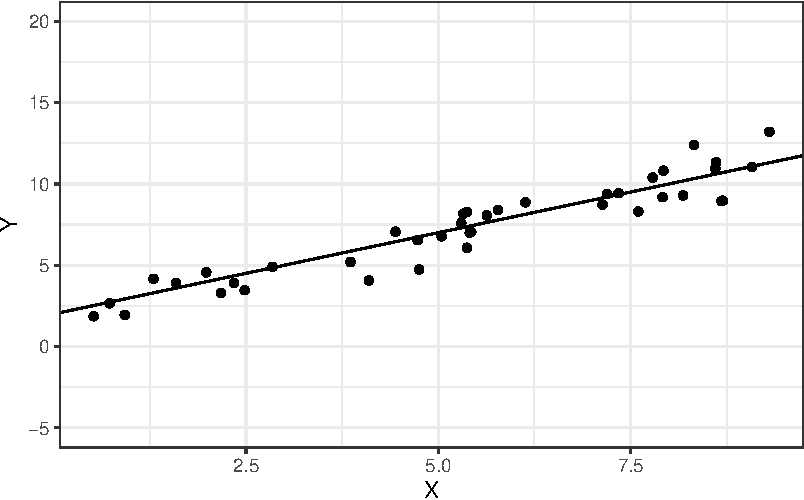
\includegraphics[width=0.75\textwidth,height=\textheight]{12-model_selection_files/figure-pdf/unnamed-chunk-1-2.pdf}
\end{center}

These are exactly the same two regression lines. But we probably have
the sense that the regression line in the second figure ``fits better''
than in the first figure, and, furthermore, that this is likely to
result in better predictions of whatever the second outcome is relative
to the first one. We'll formalize this below.

\subsection{TSS, ESS, SSR}\label{tss-ess-ssr}

SW 6.4

Let's start by defining some quantities. These will be useful for
quantifying how well the model fits the data.

\begin{itemize}
\item
  Total Sum of Squares (TSS) --- measures total variation in the data

  \[
      TSS = \sum_{i=1}^n (Y_i - \bar{Y})^2
    \]
\item
  Explained Sum of Squares (ESS) --- measures variation explained by the
  model

  \[
      ESS = \sum_{i=1}^n (\hat{Y}_i - \bar{Y})^2
    \]
\item
  Sum of Squared Residuals (SSR) --- measures ``leftover'' variation in
  the data that is not explained by the model

  \[
      SSR = \sum_{i=1}^n \hat{U}_i^2 = \sum_{i=1}^n (Y_i - \hat{Y}_i)^2
    \]
\end{itemize}

\textbf{Properties}

\begin{itemize}
\item
  A first useful property is

  \[
      TSS = ESS + SSR
    \]

  We will not prove this property though it is a useful exercise and not
  actually that challenging.
\item
  Another useful property is that \(TSS\), \(ESS\), and \(SSR\) are all
  positive --- this holds because they all involve sums of squared
  quantities.
\end{itemize}

\subsection{\texorpdfstring{\(R^2\)}{R\^{}2}}\label{r2}

SW 6.4

\(R^2\) is probably the most common measure of regression fit. It is
defined as

\[
  R^2 := \frac{ESS}{TSS}
\]

so that \(R^2\) is the fraction of the variation in \(Y\) explained by
the model. Notice that \(R^2\) is always between 0 and 1 which holds by
the two properties of \(TSS\), \(ESS\), and \(SSR\) listed in the
previous section.

\section{Model Selection}\label{model-selection-1}

SW 7.5 (note: we cover substantially more details than the textbook
about model selection)

Often, when we want to use data to make predictions, there are multiple
possible models that we could estimate to make the predictions. For
example, suppose that we are interested in predicting house prices and
we have access to data about the number of square feet, whether or not
the house has a basement, the number of bedrooms, and the number of
bathrooms. All of these are probably good variables to include in a
model to predict house prices (though it is less clear if we should
include quadratic terms, interaction terms, or other higher order
terms). But suppose we also observe some variables that are probably
irrelevant (e.g., whether the street number is odd or even) or not clear
whether they matter or not (e.g., number of ceiling fans or paint
color). It is not clear which variables we should include in the model.
An alternative way to think about this is that there would be a large
number of possible models that we could estimate here, and it is not
immediately obvious which one will predict the best.

From the previous example, it seems that in many realistic applications,
there are a large number of possible models that we could estimate to
make predictions. How should we choose which one to use?

One idea is to just throw all the data that we have into the model. In
many applications, this may not be a good idea. I'll provide a specific
example below.

Before doing that, I want to distinguish between two concepts.
Typically, what we mean we say that a model is good at making
predictions is that it is a good at making \textbf{out-of-sample}
predictions. In other words, some new observation shows up (e.g., a new
house comes on the market) with certain characteristics --- we would
like to be using a model that makes good predictions for this house.
This is a distinct concept from \textbf{in-sample} fit of the model ---
how well a model predicts for the data that it is estimated on. In the
context of prediction, one very common problem is \textbf{over-fitting}.
Over-fitting is the problem of getting predictions that are \emph{too
specific} to the particular data that you have, but then that don't work
well for new data.

{Example: }Suppose that you are interested in predicting height of
students at UGA. You consider estimating three models

\[
  \begin{aligned}
    Height &= \beta_0 + \beta_1 Male + U \\
    Height &= \beta_0 + \beta_1 Male + \beta_2 Year + U \\
    Height &= \beta_0 + \beta_1 Male + \beta_2 Year + \beta_3 Birthday + U
  \end{aligned}
\] where \(Year\) is what year in school a student is in (e.g.,
Freshman, Sophomore, etc.), and \(Birthday\) is what day of the year a
student was born on.

You also notice that \(R^2\) is greatest for the third model, in the
middle for the second model, and smallest for the first model.

The third model likely suffers from over-fitting. In particular, knowing
a student's birthday may really help you predict height in-sample. For
example, suppose that the center on the basketball team is in your
sample, and his birthday is July 15. Knowing this, you will likely be
able to make a much better prediction for this observation in your data
using Model 3 which \(\implies\) that the \(R^2\) will be much higher
for this model. But this won't help you predict well out-of-sample. If a
new person shows up whose birthday is July 15, they are unlikely to also
be a center on the basketball team which further implies that your
prediction of their height is likely to be very poor.

The previous example is about over-fitting with the idea that better
in-sample predictions can actually lead to worse out-of-sample
predictions.

\section{\texorpdfstring{Limitations of
\(R^2\)}{Limitations of R\^{}2}}\label{limitations-of-r2}

SW 6.4

\(R^2\) is a measure of in-sample fit. In fact, you can always increase
\(R^2\) by adding new variables into a model. To see this, notice that

\[
  \begin{aligned}
    R^2 &= \frac{ESS}{TSS} \\
    &= 1 - \frac{SSR}{TSS}
  \end{aligned}
\] When you add a new variable to a model, \(SSR\) cannot increase (see
explanation below). Since \(SSR\) cannot increase, it means that \(R^2\)
can only increase (or at a minimum remain unchanged) when a new
regressor is added to the model.

This means that, if you were to choose a model by \(R^2\), it would
always choose the ``kitchen-sink'' (include everything) model. But, as
we discussed above, this is likely to lead to severe over-fitting
problems. This suggests using alternative approaches to choose a model
for the purposed of prediction.

{Side-Comment:} It might not be obvious why \(SSR\) necessarily
decreases when a covariate is added to the model. Here is an
explanation. Suppose that we estimate two models (I'll include an \(i\)
subscript here and just use \(\beta\) and \(\delta\) to remind you that
the parameters are not equal to each other across models)

\[
  \begin{aligned}
  Y_i &= \hat{\beta}_0 + \hat{\beta}_1 X_{1i} + \hat{U}_{1i} \\
  Y_i &= \hat{\delta}_0 + \hat{\delta}_1 X_{1i} + \hat{\delta}_2 X_{2i} + \hat{U}_{2i}
  \end{aligned}
\] Recall that, for both models, we estimate the parameters by
minimizing the sum of squared residuals (\(SSR\)). Notice that the
second model is equivalent to the first model when \(\hat{\delta}_2=0\).
In that case, \(\hat{\delta}_0 = \hat{\beta}_0\),
\(\hat{\delta}_1 = \hat{\beta}_1\), the residuals would be exactly the
same which implies that \(SSR\) would be exactly the same across each
model. Now, for the second model, if we estimate some any value of
\(\hat{\delta}_2 \neq 0\), the reason why we would estimate that is
because it makes the \(SSR\) of the second model even lower.

This discussion means that, if we estimate \(\hat{\delta}_2=0\), then
\(SSR\) wil be the same across the first and second model, and that if
we estimate any other value for \(\hat{\delta}_2\), then \(SSR\) for the
second model will be lower than for the first model.

\section{\texorpdfstring{Adjusted
\(R^2\)}{Adjusted R\^{}2}}\label{adjusted-r2}

SW 6.4

Given the above discussion, we would like to have a way to choose a
model that doesn't necessarily always select the most complicated model.

A main way to do this is to add a \textbf{penalty} to adding more
regressors to the model. One version of this is called \textbf{adjusted
\(R^2\)}, which we will write as \(\bar{R}^2\). It is defined as

\[
  \bar{R}^2 := 1 - \underbrace{\frac{(n-1)}{(n-k)}}_{\textrm{penalty}} \frac{SSR}{TSS}
\] where \(k\) is the number of regressors included in the model (note:
we also count the intercept as a regressor here; so for example, in the
regression \(\E[Y|X_1,X_2] = \beta_0 + \beta_1 X_1 + \beta_2 X_2\),
\(k=3\)). Notice, if the penalty term were equal to 1, then this would
just be \(R^2\).

Now, let's think about what happens to \(\bar{R}^2\) when you add a new
regressor to the model.

\begin{itemize}
\item
  \(SSR \downarrow \implies \bar{R}^2 \uparrow\)
\item
  \((n-k-1) \downarrow \implies \bar{R}^2 \downarrow\)
\end{itemize}

Thus, there is a ``benefit'' and a ``cost'' to adding a new regressor.
If you are choosing among several models based on \(\bar{R}^2\), you
would choose the model that has the highest \(\bar{R}^2\). And the logic
is this: if the regressor greatly decreases \(SSR\), then the
``benefit'' of adding that regressor will tend to outweigh the ``cost''.
On the other hand, if the regressor has little effect on \(SSR\), then
the ``benefit'' of adding that regressor will tend to be smaller than
the ``cost''.

\section{AIC, BIC}\label{aic-bic}

There are other approaches to model selection that follow a similar
idea. Two of the most common ones are the Akaike Information Criteria
(AIC) and the Bayesian Information Criteria (BIC). These tend to be
somewhat better choices for model selection than \(\bar{R}^2\).

These are given by

\begin{itemize}
\tightlist
\item
  \(AIC = 2k + n \log(SSR)\)
\item
  \(BIC = k \log(n) + n \log(SSR)\)
\end{itemize}

For both AIC and BIC, you would choose the model that minimizes these.

\section{Cross-Validation}\label{cross-validation}

Another common way to choose a model is called
\textbf{cross-validation}. The idea is to mimic the out-of-sample
prediction problem using the data that we have access to.

In particular, one simple version of this is to split your data into two
parts: these are usually called the \textbf{training sample} and the
\textbf{testing sample}. Then, estimate all models under consideration
using the training sample. Given the estimated values of the parameters,
then predict the outcomes for observations in the testing sample; and
compare these predictions to the actual outcomes in the testing sample.
Choose the model that minimizes the squared prediction error in the
testing sample.

Cross-validation is a somewhat more complicated version of the same
idea. Basically, we will \emph{repeatedly} split the data into a
training sample and a testing sample, and get predictions for all
observations in our data (instead of just for a held-out testing
sample).

Here is an algorithm for cross-validation:

\begin{itemize}
\item
  Algorithm:

  \begin{itemize}
  \item
    Split the data into J \textbf{folds}
  \item
    For the jth fold, do the following:

    \begin{enumerate}
    \def\labelenumi{\arabic{enumi}.}
    \item
      Estimate the model using all observations \emph{not in} the Jth
      fold (\(\implies\) we obtain estimates
      \(\hat{\beta}_0^j, \hat{\beta}_1^j, \ldots, \hat{\beta}_k^j\))
    \item
      Predict outcomes for observations in the Jth fold using the
      estimated model from part (1): \begin{align*}
          \tilde{Y}_{ij} = \hat{\beta}_0^j + \hat{\beta}_1^j X_{1ij} + \cdots + \hat{\beta_k^j} X_{kij}
        \end{align*}
    \item
      Compute the prediction error: \begin{align*}
          \tilde{U}_{ij} = Y_{ij} - \tilde{Y}_{ij}
        \end{align*} (this is the difference between actual outcomes for
      individuals in the Jth fold and their predicted outcome based on
      the model from part (1))
    \end{enumerate}
  \item
    Do steps 1-3 for all \(J\) folds. This gives a prediction error
    \(\tilde{U}_i\) for each observation in the data
  \item
    compute the cross validation criteria (mean squared prediction
    error): \begin{align*}
    CV = \frac{1}{n} \sum_{i=1}^n \tilde{U}_{i}^2
      \end{align*}
  \item
    choose the model that produces the smallest value of \(CV\).
  \end{itemize}
\end{itemize}

Cross-validation is a good way to choose a model, but it can sometimes
be computationally challenging (because you are estimating lots of
models) --- particularly, if the models under consideration are very
complicated or there a large number of observations.

Above, we split the data into \(J\) folds. This introduces some
randomness into our model selection criteria. In particular, if you
split the data in a different way from how I split the data, then we
could choose different models. This is a somewhat undesirable feature of
a model selection criteria. One way to get around this is to set
\(J=n\). This makes it so that every observation has its own fold. This
is called \textbf{leave-one-out cross-validation}. In this case, there
is no randomness in the model selection criteria. The drawback is that
it is more computational --- in this case, you need to estimate the
model \(n\) times rather than \(J\) times.

\section{Model Averaging}\label{model-averaging}

In the case where you are considering a large number of possible models,
it is pretty common that a number of models will, by any of the above
model selection criteria, be expected to perform very similarly when
making predictions.

In this case, one strategy that usually does well in terms of making
out-of-sample predictions is \emph{model averaging}.

Suppose you have \(M\) different models, and that each model can produce
a predicted value for \(Y_i\) --- let's call the predicted value from
model \(m\), \(\hat{Y}_i^m\). Model averaging would involve obtaining a
new predicted value, call it \(\hat{Y}_i\) by computing \begin{align*}
  \hat{Y}_i = \frac{1}{M} \sum_{m=1}^M \hat{Y}_i^m
\end{align*}

\begin{itemize}
\tightlist
\item
  Usually, you would throw out models that you know predict poorly and
  only average together ones that perform reasonably well.
\end{itemize}

\section{Computation}\label{computation-9}

\(R^2\) and \(\bar{R}^2\) are both reported as output from \texttt{R}'s
\texttt{lm} command.

It is straightforward (and a useful exercise) to compute \(TSS, ESS,\)
and \(SSR\) directly. It is also straightforward to calculate \(AIC\)
and \(BIC\) --- there are probably packages that will do this for you,
but they are so easy that I suggest just calculating on your own.

The same applies to cross validation. I suspect that there are packages
available that will do this for you, but I think these are useful coding
exercises and not all that difficult. Also, if you do this yourself, it
removes any kinds of ``black box'' issues from downloading \texttt{R}
code where it may not be clear exactly what it is doing.

\bookmarksetup{startatroot}

\chapter{Machine Learning}\label{machine-learning}

\[
\newcommand{\E}{\mathbb{E}}
\renewcommand{\P}{\textrm{P}}
\let\L\relax
\newcommand{\L}{\textrm{L}} %doesn't work in .qmd, place this command at start of qmd file to use it
\newcommand{\F}{\textrm{F}}
\newcommand{\var}{\textrm{var}}
\newcommand{\cov}{\textrm{cov}}
\newcommand{\corr}{\textrm{corr}}
\newcommand{\Var}{\mathrm{Var}}
\newcommand{\Cov}{\mathrm{Cov}}
\newcommand{\Corr}{\mathrm{Corr}}
\newcommand{\sd}{\mathrm{sd}}
\newcommand{\se}{\mathrm{s.e.}}
\newcommand{\T}{T}
\newcommand{\indicator}[1]{\mathbb{1}\{#1\}}
\newcommand\independent{\perp \!\!\! \perp}
\newcommand{\N}{\mathcal{N}}
\]

\section{Machine Learning}\label{machine-learning-1}

SW 14.1, 14.2, 14.6

Some extra resources on estimating Lasso and Ridge regressions in R:

\begin{itemize}
\item
  \href{https://www.statology.org/lasso-regression-in-r/}{glmnet
  tutorial}
\item
  \href{https://cran.r-project.org/web/packages/glmnetUtils/vignettes/intro.html}{glmnetUtils
  vignette}
\end{itemize}

``Big'' Data typically means one of two things:

\begin{enumerate}
\def\labelenumi{\arabic{enumi}.}
\item
  \(n\) --- the number of observations is extremely large
\item
  \(k\) --- the number of regressors is very large
\end{enumerate}

\(n\) being large is more of a computer science problem. That said,
there are economists who think about these issues, but I think it is
still the case that it is relatively uncommon for an economist to have
\emph{so much} data that they have trouble computing their estimators.

We'll focus on the second issue --- where \(k\) is large. A main reason
that this may occur in applications is that we may be unsure of the
functional form for \(\E[Y|X_1,X_2,X_3]\). Should it include higher
order terms like \(X_1^2\) or \(X_1^3\)? Should it include interactions
like \(X_1 X_2\). Once you start proceeding this way, even if you only
have 5-10 actual covariates, \(k\) can become quite large.

As in the case of the mean, perhaps we can improve predictions by
introducing some bias while simultaneously decreasing the variance of
our predictions.

Let's suppose that we have some function that can take in regressors and
makes predictions of the outcome; we'll call this function \(\hat{f}\)
(where the ``hat'' indicates that we'll typically estimate this
function). An example would just be a regression where, for example,
\(\hat{f}(X) = \hat{\beta}_0 + \hat{\beta}_1 X_1 + \hat{\beta}_2 X_2 + \hat{\beta}_3 X_3\).
One way to evaluate how well \(\hat{f}\) makes predictions is by
considering its \textbf{mean squared prediction error}:

\[
  MSPE := \E\left[ (Y - \hat{f}(X))^2 \right]
\] \(MSPE\) quantifies the mean ``distance'' between our predictions and
actual outcomes.

Recall that, if we could just pick any function to minimize \(MSPE\), we
would set \(\hat{f}(X) = \E[Y|X]\), but generally we do not just know
what \(\E[Y|X]\) is. We can ``decompose'' MSPE into several underlying
conditions

\[
  \begin{aligned}
  MSPE &= \E\left[ \left( (Y - \E[Y|X]) - (\hat{f}(X) - \E[\hat{f}(X)|X]) - (\E[\hat{f}(X)|X] - \E[Y|X]) \right)^2 \right] \\
  &= \E\left[ (Y-\E[Y|X])^2 \right] + \E\left[ (\hat{f}(X) - \E[\hat{f}(X)|X])^2\right] + \E\left[ (\E[\hat{f}(X)|X] - \E[Y|X])^2 \right] \\
  &= \Var(U) + \E[\Var(\hat{f}(X)|X)] + \E\left[\textrm{Bias}(\hat{f}(X))^2\right]
  \end{aligned}
\] where, to understand this decomposition, the first equality just adds
and subtracts \(\E[Y|X]\) and \(\E[\hat{f}(X)|X]\). The second equality
squares the long expression from the first equality and cancels some
terms. The third equality holds where \(U := Y-\E[Y|X]\), by the
definition of (conditional) variance, and we call the last bias because
it is the difference between the mean of our prediction function
\(\hat{f}\) and \(\E[Y|X]\).

You can think of the term \(\Var(U)\) as being irreducible prediction
error --- even if we knew \(\E[Y|X]\), we wouldn't get every prediction
exactly right. But the other two terms come from having to estimate
\(\hat{f}\). The term \(\E[\Var(\hat{f}(X)X)]\) is the average variance
of our predictions across different values of \(X\). The term
\(\E\left[\textrm{Bias}(\hat{f}(X))^2\right]\) is the squared bias of
our predictions averaged across different values of \(X\). Many machine
learning estimators have the property of being biased (so that the last
term is not equal to 0), but having reduced variance relative to OLS
estimators.

To do this, we'll estimate the parameters of the model in a similar way
to what we have done before except that we'll add a \textbf{penalty}
term that gets larger as parameter estimates move further away from 0.
In particular, we consider estimates of the form

\[
  (\hat{\beta}_1, \hat{\beta}_2, \ldots, \hat{\beta}_k) = \underset{b_1,\ldots,b_k}{\textrm{argmin}} \sum_{i=1}^n  (Y_i - b_1 X_{1i} - \cdots - b_k X_{ki})^2 + \textrm{penalty}
\]

Lasso and ridge regression, which are the two approaches to machine
learning that we will talk about below, amount to different choices of
the penalty term.

{Side-Comment:} Generally, you should ``standardize'' the regressors
before implementing Lasso or Ridge regression. The \texttt{glmnet}
package does this for you by default.

\subsection{Lasso}\label{lasso}

SW 14.3

For Lasso, the penalty term is given by

\[
  \lambda \sum_{j=1}^k |b_j|
\] The absolute value on each of the \(b_j\) terms means that the
penalty function gets larger for larger values of any \(b_j\). Since we
are trying to minimize the objective function, this means that there is
a ``cost'' to choosing a larger value of \(b_j\) relative to OLS. Thus,
Lasso estimates tend to be ``shrunk'' towards 0.

\(\lambda\) is called a \textbf{tuning parameter} --- larger values of
\(\lambda\) imply that the penalty term is more important. Notice that,
if you send \(\lambda \rightarrow \infty\), then the penalty term will
be so large that you would set all the parameters to be equal to 0. On
the other hand, if you set \(\lambda=0\), then you will get the OLS
estimates (because there will be no penalty in this case). In general,
it is hard to know what is the ``right'' value for \(\lambda\), and it
is typically chosen using cross validation (this will be done
automatically for you using the \texttt{glmnet} package).

\subsection{Ridge Regression}\label{ridge-regression}

SW 14.4

For Ridge, the penalty term is given by

\[
  \lambda \sum_{j=1}^k b_j^2
\] Much of the discussion from Lasso applies here. The only difference
is that the form of the penalty is different here: \(b_j^2\) instead of
\(|b_j|\). Relative to the Lasso penalty, the Ridge penalty ``dislikes
more'' very large values of \(b_j\).

\textbf{Comparing Lasso and Ridge}

\begin{itemize}
\item
  Both \textbf{shrink} the estimated parameters towards 0. This tends to
  introduce bias into our predictions but comes with the benefit of
  reducing the variance of the predictions.
\item
  Interestingly, both Lasso and Ridge can be implemented when \(k > n\)
  (i.e., if you have more regressors than observations). This is in
  contrast to to OLS, where the parameters cannot be estimated in this
  case.
\item
  Both are generally not very computationally intensive. For ridge
  regression, we can in fact derive an explicit expression for the
  estimated \(\beta\)'s. We cannot do this with Lasso; a full discussion
  of how Lasso actually estimates the parameters is beyond the scope of
  our course, but, suffice it to say, that you can generally compute
  Lasso estimates quickly.
\item
  Lasso also performs ``model selection'' --- that is, if you use the
  Lasso, many of the estimated parameters will be set equal to 0. This
  can sometimes be an advantage. Ridge (like OLS) will generally produce
  non-zero estimates of all parameters in the model.
\end{itemize}

\subsection{Computation}\label{computation-10}

Computing Lasso and Ridge regressions is somewhat more complicated than
most other things that we have computed this semester. The main
\texttt{R} package for Lasso and Ridge regressions is the
\texttt{glmnet} package. For some reason, the syntax of the package is
somewhat different from, for example, the \texttt{lm} command. In my
view, it is often easier to use the \texttt{glmnetUtils} package, which
seems to be just a wrapper for \texttt{glmnet} but with functions that
are analogous to \texttt{lm}.

I'm just going to sketch here how you would use these functions to
estimate a Lasso or Ridge regression. In the lab later on in this
chapter, we'll do a more concrete example. Suppose that you have access
to a training dataset called \texttt{train} and a testing dataset called
\texttt{test}, you can use the \texttt{glmnetUtils} package in the
following way:

\begin{Shaded}
\begin{Highlighting}[]
\FunctionTok{library}\NormalTok{(glmnetUtils)}
\NormalTok{lasso\_model }\OtherTok{\textless{}{-}} \FunctionTok{cv.glmnet}\NormalTok{(Y }\SpecialCharTok{\textasciitilde{}}\NormalTok{ X1 }\SpecialCharTok{+}\NormalTok{ X2 }\SpecialCharTok{+}\NormalTok{ X3, }\AttributeTok{data=}\NormalTok{train, }\AttributeTok{use.model.frame=}\ConstantTok{TRUE}\NormalTok{) }\CommentTok{\# or whatever formula you want to use}
\FunctionTok{coef}\NormalTok{(lasso\_model) }\CommentTok{\# if you are interested in estimated coefficients}
\FunctionTok{predict}\NormalTok{(lasso\_model, }\AttributeTok{newdata=}\NormalTok{test) }\CommentTok{\# get predictions}

\NormalTok{ridge\_model }\OtherTok{\textless{}{-}} \FunctionTok{cv.glmnet}\NormalTok{(Y }\SpecialCharTok{\textasciitilde{}}\NormalTok{ X1 }\SpecialCharTok{+}\NormalTok{ X2 }\SpecialCharTok{+}\NormalTok{ X3, }
                         \AttributeTok{data=}\NormalTok{train, }
                         \AttributeTok{alpha=}\DecValTok{0}\NormalTok{,}
                         \AttributeTok{use.model.frame=}\ConstantTok{TRUE}\NormalTok{)}
\FunctionTok{coef}\NormalTok{(ridge\_model)}
\FunctionTok{predict}\NormalTok{(ridge\_model, }\AttributeTok{newdata=}\NormalTok{test)}
\end{Highlighting}
\end{Shaded}

It's worth making a couple of comments about this

• In terms of code, the only difference between the Lasso and Ridge, is
that for Ridge, we added the extra argument \texttt{alpha=0}. The
default value of \texttt{alpha} is 1, and that leads to a Lasso
regression (which is why didn't need to specify it for our Lasso
estimates). If you are interested, you can read more details about this
in the documentation for \texttt{glmnet} using \texttt{?glmnet}.

• Generally, if you are going to use Lasso or Ridge, then you would have
many more regressors to include than just \texttt{X1\ +\ X2\ +\ X3}. One
common way that you get more regressors is when you start to thinking
about including higher order terms or interaction terms. One way to do
this quickly is to use the \texttt{poly} function inside the formula.
For example,

\begin{Shaded}
\begin{Highlighting}[]
\NormalTok{lasso\_model2 }\OtherTok{\textless{}{-}} \FunctionTok{cv.glmnet}\NormalTok{(Y }\SpecialCharTok{\textasciitilde{}} \FunctionTok{poly}\NormalTok{(X1, X2, X3, }\AttributeTok{degree=}\DecValTok{2}\NormalTok{, }\AttributeTok{raw=}\ConstantTok{TRUE}\NormalTok{), }
                          \AttributeTok{data=}\NormalTok{train, }
                          \AttributeTok{use.model.frame=}\ConstantTok{TRUE}\NormalTok{)}
\end{Highlighting}
\end{Shaded}

would include all interactions between \(X_1\), \(X_2\) and \(X_3\) as
well as squared terms for each; if you wanted to include more
interactions and cubic terms, you could specify \texttt{degree=3}.

\section{Lab 6: Predicting Diamond
Prices}\label{lab-6-predicting-diamond-prices}

For this lab, we will try our hand at predicted diamond prices. We will
use the data set \texttt{diamond\_train} (which contains around 40,000
observations) and then see how well we can predict data from the
\texttt{diamond\_test} data.

\begin{enumerate}
\def\labelenumi{\arabic{enumi}.}
\item
  Estimate a model for \(price\) on \(carat\), \(cut\), and \(clarity\).
  Report \(R^2\), \(\bar{R}^2\), \(AIC\), and \(BIC\) for this model.
\item
  Estimate a model for \(price\) on \(carat\), \(cut\), \(clarity\),
  \(depth\), \(table\), \(x\), \(y\), and \(z\). Report \(R^2\),
  \(\bar{R}^2\), \(AIC\), and \(BIC\) for this model.
\item
  Choose any model that you would like for \(price\) and report \(R^2\),
  \(\bar{R}^2\), \(AIC\), and \(BIC\) for this model. We'll see if your
  model can predict better than either of the first two.
\item
  Use 10-fold cross validation to report an estimate of mean squared
  prediction error for each of the models from 1-3.
\item
  Based on your responses to parts 1-4, which model do you think will
  predict the best?
\item
  Use \texttt{diamond\_test} to calculate (out-of-sample) mean squared
  prediction error for each of the three models from 1-3. Which model
  performs the best out-of-sample? How does this compare to your answer
  from 5.
\item
  Use the Lasso and Ridge regression on \texttt{diamond\_train} data.
  Evaluate the predictions from each of these models by computing
  (out-of-sample) mean squared prediction error. How well did these
  models predict relative to each other and relative the models from
  1-3.
\end{enumerate}

\section{Lab 6: Solutions}\label{lab-6-solutions}

\begin{Shaded}
\begin{Highlighting}[]
\FunctionTok{load}\NormalTok{(}\StringTok{"data/diamond\_train.RData"}\NormalTok{)}

\CommentTok{\# formulas}
\NormalTok{formla1 }\OtherTok{\textless{}{-}}\NormalTok{ price }\SpecialCharTok{\textasciitilde{}}\NormalTok{ carat }\SpecialCharTok{+} \FunctionTok{as.factor}\NormalTok{(cut) }\SpecialCharTok{+} \FunctionTok{as.factor}\NormalTok{(clarity)}
\NormalTok{formla2 }\OtherTok{\textless{}{-}}\NormalTok{ price }\SpecialCharTok{\textasciitilde{}}\NormalTok{ carat }\SpecialCharTok{+} \FunctionTok{as.factor}\NormalTok{(cut) }\SpecialCharTok{+} \FunctionTok{as.factor}\NormalTok{(clarity) }\SpecialCharTok{+}\NormalTok{ depth }\SpecialCharTok{+}\NormalTok{ table }\SpecialCharTok{+}\NormalTok{ x }\SpecialCharTok{+}\NormalTok{ y }\SpecialCharTok{+}\NormalTok{ x}
\NormalTok{formla3 }\OtherTok{\textless{}{-}}\NormalTok{ price }\SpecialCharTok{\textasciitilde{}}\NormalTok{ (carat }\SpecialCharTok{+} \FunctionTok{as.factor}\NormalTok{(cut) }\SpecialCharTok{+} \FunctionTok{as.factor}\NormalTok{(clarity) }\SpecialCharTok{+}\NormalTok{ depth }\SpecialCharTok{+}\NormalTok{ table }\SpecialCharTok{+}\NormalTok{ x }\SpecialCharTok{+}\NormalTok{ y }\SpecialCharTok{+}\NormalTok{ x)}\SpecialCharTok{\^{}}\DecValTok{2}

\CommentTok{\# estimate each model}
\NormalTok{mod1 }\OtherTok{\textless{}{-}} \FunctionTok{lm}\NormalTok{(formla1, }\AttributeTok{data=}\NormalTok{diamond\_train)}
\NormalTok{mod2 }\OtherTok{\textless{}{-}} \FunctionTok{lm}\NormalTok{(formla2, }\AttributeTok{data=}\NormalTok{diamond\_train)}
\NormalTok{mod3 }\OtherTok{\textless{}{-}} \FunctionTok{lm}\NormalTok{(formla3, }\AttributeTok{data=}\NormalTok{diamond\_train)}

\NormalTok{mod\_sel }\OtherTok{\textless{}{-}} \ControlFlowTok{function}\NormalTok{(formla) \{}
\NormalTok{  mod }\OtherTok{\textless{}{-}} \FunctionTok{lm}\NormalTok{(formla, }\AttributeTok{data=}\NormalTok{diamond\_train)}
\NormalTok{  r.squared }\OtherTok{\textless{}{-}} \FunctionTok{summary}\NormalTok{(mod)}\SpecialCharTok{$}\NormalTok{r.squared}
\NormalTok{  adj.r.squared }\OtherTok{\textless{}{-}} \FunctionTok{summary}\NormalTok{(mod)}\SpecialCharTok{$}\NormalTok{adj.r.squared}

\NormalTok{  n }\OtherTok{\textless{}{-}} \FunctionTok{nrow}\NormalTok{(diamond\_train)}
\NormalTok{  uhat }\OtherTok{\textless{}{-}} \FunctionTok{resid}\NormalTok{(mod)}
\NormalTok{  ssr }\OtherTok{\textless{}{-}} \FunctionTok{sum}\NormalTok{(uhat}\SpecialCharTok{\^{}}\DecValTok{2}\NormalTok{)}
\NormalTok{  k }\OtherTok{\textless{}{-}} \FunctionTok{length}\NormalTok{(}\FunctionTok{coef}\NormalTok{(mod))}
\NormalTok{  aic }\OtherTok{\textless{}{-}} \DecValTok{2}\SpecialCharTok{*}\NormalTok{k }\SpecialCharTok{+}\NormalTok{ n}\SpecialCharTok{*}\FunctionTok{log}\NormalTok{(ssr)}
\NormalTok{  bic }\OtherTok{\textless{}{-}}\NormalTok{ k}\SpecialCharTok{*}\FunctionTok{log}\NormalTok{(n) }\SpecialCharTok{+}\NormalTok{ n}\SpecialCharTok{*}\FunctionTok{log}\NormalTok{(ssr)}

  \CommentTok{\# show results}
\NormalTok{  result }\OtherTok{\textless{}{-}}\NormalTok{ tidyr}\SpecialCharTok{::}\FunctionTok{tibble}\NormalTok{(r.squared, adj.r.squared, aic, bic)}
  \FunctionTok{return}\NormalTok{(result)}
\NormalTok{\}}

\NormalTok{res1 }\OtherTok{\textless{}{-}} \FunctionTok{mod\_sel}\NormalTok{(formla1)}
\NormalTok{res2 }\OtherTok{\textless{}{-}} \FunctionTok{mod\_sel}\NormalTok{(formla2)}
\NormalTok{res3 }\OtherTok{\textless{}{-}} \FunctionTok{mod\_sel}\NormalTok{(formla3)}

\FunctionTok{round}\NormalTok{(}\FunctionTok{rbind.data.frame}\NormalTok{(res1, res2, res3),}\DecValTok{3}\NormalTok{)}
\end{Highlighting}
\end{Shaded}

\begin{verbatim}
# A tibble: 3 x 4
  r.squared adj.r.squared      aic      bic
      <dbl>         <dbl>    <dbl>    <dbl>
1     0.898         0.898 1104188. 1104301.
2     0.9           0.9   1103499. 1103647.
3     0.928         0.928 1089372. 1090328.
\end{verbatim}

\begin{Shaded}
\begin{Highlighting}[]
\CommentTok{\# k{-}fold cross validation}

\CommentTok{\# setup data}
\NormalTok{k }\OtherTok{\textless{}{-}} \DecValTok{10}
\NormalTok{n }\OtherTok{\textless{}{-}} \FunctionTok{nrow}\NormalTok{(diamond\_train)}
\NormalTok{diamond\_train}\SpecialCharTok{$}\NormalTok{fold }\OtherTok{\textless{}{-}} \FunctionTok{sample}\NormalTok{(}\DecValTok{1}\SpecialCharTok{:}\NormalTok{k, }\AttributeTok{size=}\NormalTok{n, }\AttributeTok{replace=}\ConstantTok{TRUE}\NormalTok{)}
\NormalTok{diamond\_train}\SpecialCharTok{$}\NormalTok{id }\OtherTok{\textless{}{-}} \DecValTok{1}\SpecialCharTok{:}\NormalTok{n}

\NormalTok{cv\_mod\_sel }\OtherTok{\textless{}{-}} \ControlFlowTok{function}\NormalTok{(formla) \{}
\NormalTok{  u.squared }\OtherTok{\textless{}{-}} \FunctionTok{rep}\NormalTok{(}\ConstantTok{NA}\NormalTok{, n)}
  \ControlFlowTok{for}\NormalTok{ (i }\ControlFlowTok{in} \DecValTok{1}\SpecialCharTok{:}\NormalTok{k) \{}
\NormalTok{    this.train }\OtherTok{\textless{}{-}} \FunctionTok{subset}\NormalTok{(diamond\_train, fold }\SpecialCharTok{!=}\NormalTok{ i)}
\NormalTok{    this.test }\OtherTok{\textless{}{-}} \FunctionTok{subset}\NormalTok{(diamond\_train, fold }\SpecialCharTok{==}\NormalTok{ i)}
\NormalTok{    this.id }\OtherTok{\textless{}{-}}\NormalTok{ this.test}\SpecialCharTok{$}\NormalTok{id}
\NormalTok{    cv\_reg }\OtherTok{\textless{}{-}} \FunctionTok{lm}\NormalTok{(formla,}
              \AttributeTok{data=}\NormalTok{this.train)}
\NormalTok{    pred }\OtherTok{\textless{}{-}} \FunctionTok{predict}\NormalTok{(cv\_reg, }\AttributeTok{newdata=}\NormalTok{this.test)}
\NormalTok{    u }\OtherTok{\textless{}{-}}\NormalTok{ this.test}\SpecialCharTok{$}\NormalTok{price }\SpecialCharTok{{-}}\NormalTok{ pred}
\NormalTok{    u.squared[this.id] }\OtherTok{\textless{}{-}}\NormalTok{ u}\SpecialCharTok{\^{}}\DecValTok{2}
\NormalTok{  \}}
\NormalTok{  cv }\OtherTok{\textless{}{-}} \FunctionTok{sqrt}\NormalTok{(}\FunctionTok{mean}\NormalTok{(u.squared))}
  \FunctionTok{return}\NormalTok{(cv)}
\NormalTok{\}}

\NormalTok{cv\_res1 }\OtherTok{\textless{}{-}} \FunctionTok{cv\_mod\_sel}\NormalTok{(formla1)}
\NormalTok{cv\_res2 }\OtherTok{\textless{}{-}} \FunctionTok{cv\_mod\_sel}\NormalTok{(formla2)}
\NormalTok{cv\_res3 }\OtherTok{\textless{}{-}} \FunctionTok{cv\_mod\_sel}\NormalTok{(formla3)}

\NormalTok{res1 }\OtherTok{\textless{}{-}} \FunctionTok{cbind.data.frame}\NormalTok{(res1, }\AttributeTok{cv=}\NormalTok{cv\_res1)}
\NormalTok{res2 }\OtherTok{\textless{}{-}} \FunctionTok{cbind.data.frame}\NormalTok{(res2, }\AttributeTok{cv=}\NormalTok{cv\_res2)}
\NormalTok{res3 }\OtherTok{\textless{}{-}} \FunctionTok{cbind.data.frame}\NormalTok{(res3, }\AttributeTok{cv=}\NormalTok{cv\_res3)}

\FunctionTok{round}\NormalTok{(}\FunctionTok{rbind.data.frame}\NormalTok{(res1, res2, res3),}\DecValTok{3}\NormalTok{)}
\end{Highlighting}
\end{Shaded}

\begin{verbatim}
  r.squared adj.r.squared     aic     bic       cv
1     0.898         0.898 1104188 1104301 1365.944
2     0.900         0.900 1103499 1103647 1400.933
3     0.928         0.928 1089372 1090328 2223.032
\end{verbatim}

\begin{Shaded}
\begin{Highlighting}[]
\CommentTok{\# lasso and ridge}
\FunctionTok{library}\NormalTok{(glmnet)}
\FunctionTok{library}\NormalTok{(glmnetUtils)}

\NormalTok{lasso\_res }\OtherTok{\textless{}{-}} \FunctionTok{cv.glmnet}\NormalTok{(formla3, }\AttributeTok{data=}\NormalTok{diamond\_train, }\AttributeTok{alpha=}\DecValTok{1}\NormalTok{)}
\NormalTok{ridge\_res }\OtherTok{\textless{}{-}} \FunctionTok{cv.glmnet}\NormalTok{(formla3, }\AttributeTok{data=}\NormalTok{diamond\_train, }\AttributeTok{alpha=}\DecValTok{0}\NormalTok{)}

\CommentTok{\# out of sample predictions}

\FunctionTok{load}\NormalTok{(}\StringTok{"data/diamond\_test.RData"}\NormalTok{)}

\CommentTok{\# compute prediction errors with test data}
\NormalTok{u1 }\OtherTok{\textless{}{-}}\NormalTok{ diamond\_test}\SpecialCharTok{$}\NormalTok{price }\SpecialCharTok{{-}} \FunctionTok{predict}\NormalTok{(mod1, }\AttributeTok{newdata=}\NormalTok{diamond\_test)}
\NormalTok{u2 }\OtherTok{\textless{}{-}}\NormalTok{ diamond\_test}\SpecialCharTok{$}\NormalTok{price }\SpecialCharTok{{-}} \FunctionTok{predict}\NormalTok{(mod2, }\AttributeTok{newdata=}\NormalTok{diamond\_test)}
\NormalTok{u3 }\OtherTok{\textless{}{-}}\NormalTok{ diamond\_test}\SpecialCharTok{$}\NormalTok{price }\SpecialCharTok{{-}} \FunctionTok{predict}\NormalTok{(mod3, }\AttributeTok{newdata=}\NormalTok{diamond\_test)}
\NormalTok{u\_lasso }\OtherTok{\textless{}{-}}\NormalTok{ diamond\_test}\SpecialCharTok{$}\NormalTok{price }\SpecialCharTok{{-}} \FunctionTok{predict}\NormalTok{(lasso\_res, }\AttributeTok{newdata=}\NormalTok{diamond\_test)}
\NormalTok{u\_ridge }\OtherTok{\textless{}{-}}\NormalTok{ diamond\_test}\SpecialCharTok{$}\NormalTok{price }\SpecialCharTok{{-}} \FunctionTok{predict}\NormalTok{(ridge\_res, }\AttributeTok{newdata=}\NormalTok{diamond\_test)}

\CommentTok{\# compute root mean squared prediction errors}
\NormalTok{rmspe1 }\OtherTok{\textless{}{-}} \FunctionTok{sqrt}\NormalTok{(}\FunctionTok{mean}\NormalTok{(u1}\SpecialCharTok{\^{}}\DecValTok{2}\NormalTok{))}
\NormalTok{rmspe2 }\OtherTok{\textless{}{-}} \FunctionTok{sqrt}\NormalTok{(}\FunctionTok{mean}\NormalTok{(u2}\SpecialCharTok{\^{}}\DecValTok{2}\NormalTok{))}
\NormalTok{rmspe3 }\OtherTok{\textless{}{-}} \FunctionTok{sqrt}\NormalTok{(}\FunctionTok{mean}\NormalTok{(u3}\SpecialCharTok{\^{}}\DecValTok{2}\NormalTok{))}
\NormalTok{rmspe\_lasso }\OtherTok{\textless{}{-}} \FunctionTok{sqrt}\NormalTok{(}\FunctionTok{mean}\NormalTok{(u\_lasso}\SpecialCharTok{\^{}}\DecValTok{2}\NormalTok{))}
\NormalTok{rmspe\_ridge }\OtherTok{\textless{}{-}} \FunctionTok{sqrt}\NormalTok{(}\FunctionTok{mean}\NormalTok{(u\_ridge}\SpecialCharTok{\^{}}\DecValTok{2}\NormalTok{))}

\CommentTok{\# report results}
\NormalTok{rmspe }\OtherTok{\textless{}{-}} \FunctionTok{data.frame}\NormalTok{(}\AttributeTok{mod1=}\NormalTok{rmspe1, }\AttributeTok{mod2=}\NormalTok{rmspe2, }\AttributeTok{mod3=}\NormalTok{rmspe3, }\AttributeTok{lasso=}\NormalTok{rmspe\_lasso, }\AttributeTok{ridge=}\NormalTok{rmspe\_ridge)}
\FunctionTok{round}\NormalTok{(rmspe,}\DecValTok{3}\NormalTok{)}
\end{Highlighting}
\end{Shaded}

\begin{verbatim}
     mod1    mod2    mod3   lasso   ridge
1 856.014 785.171 616.996 671.448 794.276
\end{verbatim}

\section{Extra Questions}\label{extra-questions-4}

\begin{enumerate}
\def\labelenumi{\arabic{enumi}.}
\item
  What are some drawbacks of using \(R^2\) as a model selection tool?
\item
  For AIC and BIC, we choose the model that minimizes these (rather than
  maximizes them). Why?
\item
  Does AIC or BIC tend to pick ``more complicated'' models? What is the
  reason for this?
\item
  Suppose you are interested in predicting some outcome \(Y\) and have
  access to covariates \(X_1\), \(X_2\), and \(X_3\). You estimate the
  following two models \begin{align*}
    Y &= 30 + 4 X_1 - 2 X_2 - 10 X_3, \qquad R^2=0.5, AIC=3421 \\
    Y &= 9 + 2 X_1 - 3 X_2 - 2 X_3 + 2 X_1^2 + 1 X_2^2 - 4 X_3^2 + 2 X_1 X_2, \qquad R^2 = 0.75, AIC=4018
  \end{align*}

  \begin{enumerate}
  \def\labelenumii{\alph{enumii})}
  \item
    Which model seems to be predicting better? Explain why.
  \item
    Using the model that is predicting better, what would be your
    prediction for \(Y\) when \(X_1=10, X_2=1, X_3=5\)?
  \end{enumerate}
\item
  In Lasso and Ridge regressions, it is common to ``standardize'' the
  regressors before estimating the model (e.g., the \texttt{glmnet} does
  this automatically for you). What is the reason for doing this?
\item
  In Lasso and Ridge regressions, the penalty term lead to ``shrinking''
  the estimated parameters in the model towards 0. This tends to
  introduce bias while reducing variance. Why can introducing bias while
  reducing variance potentially lead to better predictions? Does this
  argument always apply or just apply in some cases? Explain.
\item
  In Lasso and Ridge regressions, the penalty term depends on the tuning
  parameter \(\lambda\).

  \begin{enumerate}
  \def\labelenumii{\alph{enumii})}
  \item
    How is this tuning parameter often chosen in practice? Why does it
    make sense to choose it in this way?
  \item
    What would happen to the estimated coefficients when \(\lambda=0\)?
  \item
    What would happen to the estimated coefficients as
    \(\lambda \rightarrow \infty\)?
  \end{enumerate}
\end{enumerate}

\section{Answers to Some Extra
Questions}\label{answers-to-some-extra-questions-1}

\textbf{Answer to Question 4}

\begin{enumerate}
\def\labelenumi{\alph{enumi})}
\item
  The first model appears to be predicting better because the AIC is
  lower. {[}Also, notice that \(R^2\) is higher in the second model, but
  this is by construction because it includes extra terms relative to
  the first model which implies that it will fit at least as well
  in-sample as the first model, but may be suffering from
  over-fitting.{]}
\item
  \begin{align*}
     \hat{Y} &= 30 + 4 (10) - 2 (1) - 10 (5) \\
     &= 18
   \end{align*}
\end{enumerate}

\textbf{Answer to Question 7}

\begin{enumerate}
\def\labelenumi{\alph{enumi})}
\item
  The tuning parameter is often chosen via cross validation. It makes
  sense to choose it this way because this is effectively choosing a
  value of \(\lambda\) that is making good pseudo-out-of-sample
  predictions. As we will see below, if you make bad choices of
  \(\lambda\), that could result in very poor predictions.
\item
  When \(\lambda=0\), there would effectively be no penalty term and,
  therefore, the estimated parameters would coincide with the OLS
  estimates.
\item
  When \(\lambda \rightarrow \infty\), the penalty term would overwhelm
  the term corresponding to minimizing SSR. This would result in setting
  all the estimated parameters to be equal to 0. This extreme approach
  is likely to lead to very poor predictions.
\end{enumerate}

\part{Causal Inference}

\bookmarksetup{startatroot}

\chapter{Concepts}\label{concepts}

\[
\newcommand{\E}{\mathbb{E}}
\renewcommand{\P}{\textrm{P}}
\let\L\relax
\newcommand{\L}{\textrm{L}} %doesn't work in .qmd, place this command at start of qmd file to use it
\newcommand{\F}{\textrm{F}}
\newcommand{\var}{\textrm{var}}
\newcommand{\cov}{\textrm{cov}}
\newcommand{\corr}{\textrm{corr}}
\newcommand{\Var}{\mathrm{Var}}
\newcommand{\Cov}{\mathrm{Cov}}
\newcommand{\Corr}{\mathrm{Corr}}
\newcommand{\sd}{\mathrm{sd}}
\newcommand{\se}{\mathrm{s.e.}}
\newcommand{\T}{T}
\newcommand{\indicator}[1]{\mathbb{1}\{#1\}}
\newcommand\independent{\perp \!\!\! \perp}
\newcommand{\N}{\mathcal{N}}
\]

For the remainder of the semester, we will talk about methods for
understanding the \textbf{causal effect} of one variable on another.

Let's start with an example. Suppose we were interested in understanding
the causal effect of attending college on earnings. We know a lot about
calculating averages, so let's consider calculating average earnings of
those who went to college and comparing that to the average earnings of
those who didn't go to college. Let's use the data that we used all the
way back in Chapter 2 to make this calculation.

\begin{Shaded}
\begin{Highlighting}[]
\FunctionTok{load}\NormalTok{(}\StringTok{"us\_data.RData"}\NormalTok{)}

\NormalTok{col\_earnings }\OtherTok{\textless{}{-}} \FunctionTok{mean}\NormalTok{(}\FunctionTok{subset}\NormalTok{(us\_data, educ }\SpecialCharTok{\textgreater{}=} \DecValTok{16}\NormalTok{)}\SpecialCharTok{$}\NormalTok{incwage)}
\NormalTok{non\_col\_earnings }\OtherTok{\textless{}{-}} \FunctionTok{mean}\NormalTok{(}\FunctionTok{subset}\NormalTok{(us\_data, educ }\SpecialCharTok{\textless{}} \DecValTok{16}\NormalTok{)}\SpecialCharTok{$}\NormalTok{incwage)}

\FunctionTok{round}\NormalTok{(}\FunctionTok{data.frame}\NormalTok{(col\_earnings, }
\NormalTok{                 non\_col\_earnings, }
                 \AttributeTok{diff=}\NormalTok{(col\_earnings}\SpecialCharTok{{-}}\NormalTok{non\_col\_earnings)),}\DecValTok{3}\NormalTok{)}
\end{Highlighting}
\end{Shaded}

\begin{verbatim}
  col_earnings non_col_earnings     diff
1     87306.33         40557.28 46749.05
\end{verbatim}

This seems to be a huge difference. We are used to calling this
difference a partial effect of going to college, but should we call it
\emph{the causal effect} or an average causal effect across individuals?
Probably no. The main reason is that earnings of individuals who went to
college may have been different from individuals that didn't go to
college even if no one went to college. Another way to say this is that
there are a number of other things besides college that affect a
person's earnings (age, race, IQ, ``ability'', ``hardworking-ness'',
luck, etc.). If these are also correlated with whether or not a person
goes to college (you would think that at least some of these are), then
that would make it hard to interpret our simple difference-in-means as a
causal effect.

Before we move on, let me give some more examples of causal questions
that may be of interest to economists:

\begin{itemize}
\item
  Causal effects of economic policies

  \begin{itemize}
  \item
    What was the causal effect of a country raising its interest rate on
    GDP or employment?
  \item
    What was the causal effect of a change in the minimum wage on
    employment?
  \item
    What was the causal effect of changing voter ID laws on the number
    of ballots cast?
  \end{itemize}
\item
  Causal effects of individual/firm choices

  \begin{itemize}
  \item
    What was the causal effect of a price increase on quantity demanded?
  \item
    What was the causal effect of changing a product attribute on some
    outcome of interest (e.g., changing the font type on clicks on
    Google ads)?
  \item
    What was the causal effect of a new cholesterol medication on
    cholesterol levels?
  \item
    What was the causal effect of a job training program on wages?
  \end{itemize}
\end{itemize}

You could easily come up with many others too. A large fraction of the
questions that researchers in economics try to address are ultimately
about sorting out these sorts of causal effects.

For terminology, we'll refer to the variable that we are interested in
understanding its causal effect (going to college in the earlier
example) as the \textbf{treatment}. For simplicity, we will mostly focus
on the case where the treatment is binary. We will use \(D_i\) to denote
the treatment, so that \(D_i=1\) if individual \(i\) participates in the
treatment and \(D_i=0\) if individual \(i\) does not participate in the
treatment.

Example: SW 13.3

\section{Potential Outcomes}\label{potential-outcomes}

SW 13.1

A powerful tool for thinking about causal effects is
\textbf{counterfactual reasoning}. For individuals that participate in
the treatment, we observe what their outcome is given that they
participated in the treatment. But we don't observe what their outcome
would have been if they had not participated in the treatment. For
example, among those that went to college, we don't observe what their
earnings would have been if they had not gone to college. For those that
don't participate in the treatment, we face the opposite problem --- we
don't observe what their outcome would have been if they had
participated in the treatment.

We'll relate causal inference to the problem of trying to figure out
what outcomes individuals that participated in the treatment would have
experienced if they had \emph{not} participated in the treatment (at
least on average) and/or figuring out what outcomes individuals that did
not participated in the treatment would have experienced if they
\emph{had} participated in the treatment.

To do this, let's introduce somewhat more formal notation/terminology.

\textbf{Treated potential outcome}: \(Y_i(1)\), the outcome an
individual \emph{would experience} if they participated in the treatment

\textbf{Untreated potential outcome}: \(Y_i(0)\), the outcome an
individual \emph{would experience} if they did not participate in the
treatment

For individuals that participate in the treatment, we observe \(Y_i(1)\)
(but not \(Y_i(0)\)). For individuals that do not participate in the
treatment, we observe \(Y_i(0)\) (but not \(Y_i(1)\)). Another way to
write this is that the observed outcome, \(Y_i\) is given by
\begin{align*}
  Y_i = D_i Y_i(1) + (1-D_i) Y_i(0)
\end{align*}

We can think about the individual-level effect of participating in the
treatment: \begin{align*}
  TE_i = Y_i(1) - Y_i(0)
\end{align*}

Considering the difference between treated and untreated potential
outcomes is a very natural (and, I think, helpful) way to think about
causality. The causal effect of the treatment is the difference between
the outcome that an individual would experience if they participate in
the treatment relative to what they would experience if they did not
participate in the treatment.

This notation also makes it clear that we are allowing for
\textbf{treatment effect heterogenity} --- the effect of participating
in the treatment can vary across different individuals.

That said, most researchers essentially give up on trying to figure out
individual level treatment effects. It is not so much that these are not
interesting, more it is just that these are very hard to figure out.
Take, for example, going to college, and suppose we are interested in
the causal effect of going to college on a person's earnings. I went to
college, so I know what my \(Y(1)\) is, but I don't know what my
\(Y(0)\) is --- and, I'd even have a hard time coming with a good guess
as to what it might be.

\section{Parameters of Interest}\label{parameters-of-interest}

Instead of going for individual-level effects of participating in the
treatment, most researchers instead go for more aggregated parameters.
The two most common ones are the Average Treatment Effect (ATE) and
Average Treatment Effect on the Treated (ATT).

\begin{align*}
  ATE = \E[Y(1) - Y(0)] \qquad \textrm{and} \qquad ATT = \E[Y(1)-Y(0) | D=1]
\end{align*} \(ATE\) is the difference between treated potential
outcomes and untreated potential outcomes, on average, and for the
entire population. \(ATT\) is the difference between treated and
untreated potential outcomes, on average, conditional on being in the
treated group.

We will mostly focus on \(ATT\).

It is worth considering the challenges for learning about \(ATT\). In
particular, notice that we can write \begin{align*}
  ATT = \E[Y(1)|D=1] - \E[Y(0)|D=1]
\end{align*} and consider these term separately

\begin{itemize}
\item
  \(\E[Y(1)|D=1]\) is the average treated potential outcome among the
  treated group. But we observe treated potential outcomes for the
  treated group \(\implies \E[Y(1)|D=1] = \E[Y|D=1]\). In other words,
  if we want to estimate this component of the \(ATT\), we can just look
  right at the data and compute the average outcome experienced by
  individuals in the treated group.
\item
  \(\E[Y(0)|D=1]\) is the average untreated potential outcome among the
  treated group. This is (potentially much) more challenging than the
  first term because we do not observe untreated potential outcomes
  among the treated group. But, in order to learn about the \(ATT\), we
  will have to \emph{somehow} deal with this term. I will provide a
  number of strategies below, but it is important to remember that this
  is a major challenge, and their may not be a good solution.
\end{itemize}

{Side-Comment:} I think it is also worth clearly pointing out that,
while I am a big believer in the power/usefulness of using data to try
to answer questions in economics, the above discussion suggests that
there are a number of questions that we may just not be able to answer.
In economics jargon, this amounts to an \textbf{identification problem}
--- in other words, there may be competing theories of the world which
the available data is not able to distinguish among. I probably do not
emphasize this issue enough in our class, but it is something that you
should remember --- there may be a large number of causal questions that
we'd be interested in answering, but where it is not possible to answer
them (at least given the information that we have available).

\bookmarksetup{startatroot}

\chapter{Experiments}\label{experiments}

\[
\newcommand{\E}{\mathbb{E}}
\renewcommand{\P}{\textrm{P}}
\let\L\relax
\newcommand{\L}{\textrm{L}} %doesn't work in .qmd, place this command at start of qmd file to use it
\newcommand{\F}{\textrm{F}}
\newcommand{\var}{\textrm{var}}
\newcommand{\cov}{\textrm{cov}}
\newcommand{\corr}{\textrm{corr}}
\newcommand{\Var}{\mathrm{Var}}
\newcommand{\Cov}{\mathrm{Cov}}
\newcommand{\Corr}{\mathrm{Corr}}
\newcommand{\sd}{\mathrm{sd}}
\newcommand{\se}{\mathrm{s.e.}}
\newcommand{\T}{T}
\newcommand{\indicator}[1]{\mathbb{1}\{#1\}}
\newcommand\independent{\perp \!\!\! \perp}
\newcommand{\N}{\mathcal{N}}
\]

An experiment is often called the ``gold standard'' for causal
inference. In particular, here, we are thinking about the case where
participation in the treatment is randomly assigned --- something like:
people who show up to possibly participate in the treatment, someone
flips a coin, and if the coin comes up heads then the person
participates in the treatment or, if tails, they do not participate in
the treatment.

Random assignment means that participating in the treatment is
independent of potential outcomes, by construction. We can write this in
math as \begin{align*}
  (Y(1), Y(0)) \independent D
\end{align*} For our purposes, this also implies that \begin{align*}
  \E[Y(0)|D=1] = \E[Y(0)|D=0] = \E[Y|D=0]
\end{align*} In other words, under random assignment, the average
untreated potential among the treated group is equal to the average
untreated potential outcome among the untreated group (this is the first
equality). This is helpful because untreated potential outcomes are
observed for those in the untreated group (this is the second equality).

Thus, under random assignment, \begin{align*}
  ATT = \E[Y|D=1] - \E[Y|D=0]
\end{align*} In other words, the \(ATT\) is just the difference in
(population) average outcomes among the treated group relative to
average outcomes among the untreated group.

The natural way to estimate the ATT under random assignment is
\begin{align*}
  \widehat{ATT} = \bar{Y}_{D=1} - \bar{Y}_{D=0}
\end{align*} i.e., as we have done many times before, in order to
estimate the parameter of interest, we just replace population averages
with sample averages.

\section{Estimating ATT with a
Regression}\label{estimating-att-with-a-regression}

It is also often convenient to introduce a regression based estimator of
the ATT. This is primarily convenient as it will allow us to leverage
all the things we already know about regressions, and, particularly, we
it will immediately provide us with standard errors, t-statistics, etc.

In order to do this, let's introduce the following assumption:

\textbf{Treatment Effect Homogeneity}: \(Y_i(1) - Y_i(0) = \alpha\) (and
\(\alpha\) does not vary across individuals).

This is a potentially quite unrealistic assumption; I'll make some
additional comments about it below, but, for now, let's just go with it.

Notice that we can also write \begin{align*}
  Y_i(0) = \beta_0 + U_i
\end{align*} where \(\E[U|D=0] = \E[U|D=1] = 0\) (this holds under
random assignment since random assignment implies that treated and
untreated individuals do not have systematically different untreated
potential outcomes)

Recalling the definition of the observed outcome, notice that
\begin{align*}
  Y_i &= D_i Y_i(1) + (1-D_i) Y_i(0) \\
  &= D_i (Y_i(1) - Y_i(0)) + Y_i(0) \\
  &= \alpha D_i + \beta_0 + U_i
\end{align*} where the second equality just involves re-arranging terms,
and the third equality holds under treatment effect homogeneity and
using the expression for \(Y_i(0)\) in the previous equation.

This suggests running a regression of the observed \(Y_i\) on \(D_i\)
and interpreting the estimated version of \(\alpha\) as an estimate of
the causal effect of participating in the treatment (and you can pick up
standard errors, etc. from the regression output) --- this is very
convenient.

The previous discussion invoked the extra condition of treatment effect
homogeneity. I want to point out some things related to this now. In the
above regression model, we can alternatively (and equivalently) write it
as \begin{align*}
  \E[Y|D] = \beta_0 + \alpha D
\end{align*} Now plug in particular values for \(D\): \begin{align*}
  \E[Y|D=0] = \beta_0 \qquad \textrm{and} \qquad \E[Y|D=1] = \beta_0 + \alpha
\end{align*} Subtracting the second equation from the first implies that
\begin{align*}
  \alpha = \E[Y|D=1] - \E[Y|D=0]
\end{align*} but notice that this is exactly what the \(ATT\) is equal
to under random assignment. Thus, it is worth pointing out that,
although we imposed the assumption of treatment effect homogeneity to
arrive at the regression equation, our regression is ``robust'' to
treatment effect heterogeneity.

\section{Internal and External
Validity}\label{internal-and-external-validity}

SW 13.2

Although experiments, when they are available, are considered the gold
standard of causal inference, there are some ways they can go wrong.

An experiment is said to be \textbf{internally valid} if inferences
about causal effects are valid for the population being studied.

An experiment is said to be \textbf{externally valid} if inferences
about causal effects can be generalized from the study setting to other
populations/time periods/settings.

Generally, its easier for an experiment to be internally valid than
externally valid, but there are a number of ``threats'' to both internal
and external validity.

Threats to internal validity:

\begin{itemize}
\item
  Failure to randomize --- individuals weren't actually randomized into
  the treatment. This seems trivial, but some famous examples include
  experiments that assigned treatment participation by the first letter
  of a person's last name. It turns out that this can be correlated with
  a number of other things (violating the random assignment assumption)

  \begin{itemize}
  \tightlist
  \item
    As a side-comment, random treatment assignment implies that
    treatment should be uncorrelated with other covariates (e.g., race,
    sex, etc.) and this can be used as a way to check if the treatment
    was really randomly assigned.
  \end{itemize}
\item
  Failure to follow treatment protocol --- Individuals assigned to
  participate in the treatment don't participate or vice versa.

  \begin{itemize}
  \tightlist
  \item
    This is actually a pretty common problem. A leading example would be
    in the context of an experimental drug where patients who were
    assigned the placebo somehow to convince the doctor to give them the
    real drug.
  \end{itemize}
\item
  Attrition --- subjects non-randomly drop out of the sample
\item
  Placebo effects --- Participating in an experiment can cause changes
  in behavior/outcomes.

  \begin{itemize}
  \tightlist
  \item
    This is a main reason that medical experiments are often
    ``double-blind''
  \end{itemize}
\item
  Small sample sizes --- Experiments can be expensive to run and
  therefore often include only a small number of observations, and,
  therefore, may be less able to detect small effects of a treatment
\item
  Experiments can sometimes be unethical

  \begin{itemize}
  \tightlist
  \item
    The 2019 Nobel prize in economics was awarded for experiments in
    developing countries. Some of these experiments were somewhat
    controversial (e.g., randomly assigning some schools extra resources
    and randomly giving glasses to some students but not others).
  \end{itemize}
\end{itemize}

Threats to External Validity:

\begin{itemize}
\item
  Nonrepresentative samples --- The population that is willing to
  participate in an experiment many be substantially different from the
  overall population.

  \begin{itemize}
  \tightlist
  \item
    A closely related problem is that the economic environment may
    change across time and/or space which means that effects of some
    treatment might be different in different time periods or locations
  \end{itemize}
\item
  Nonrepresentative program/policy --- The policy in an experiment may
  be different from other policies being considered

  \begin{itemize}
  \tightlist
  \item
    For example, the Perry Preschool Project was an experiment that
    provided intensive pre-school program that seems to have had large
    and long-lasting effects on participants. It is not clear if these
    results should apply to less intensive programs like Head Start.
  \end{itemize}
\item
  General equilibrium effects --- Expanding policies may alter the
  ``state of the world'' in a way that an experiment wouldn't (e.g., the
  effects of a local minimum wage change could be different from a
  country-wide minimum wage change)
\end{itemize}

\section{Example: Project STAR}\label{example-project-star}

Project STAR was a an experiment in Tennessee in 1980s on the effects of
smaller class sizes on student performance where students and teachers
were randomly assigned to be in a small class, a regular class, or a
regular class with an aide. In this example, we'll study the causal
effect of being in a small class on reading test scores.

\begin{Shaded}
\begin{Highlighting}[]
\FunctionTok{data}\NormalTok{(}\StringTok{"Star"}\NormalTok{, }\AttributeTok{package=}\StringTok{"Ecdat"}\NormalTok{)}

\CommentTok{\# limit data to small class or regular class}
\CommentTok{\# this drops the other category of regular class size with an aide}
\NormalTok{Star }\OtherTok{\textless{}{-}} \FunctionTok{subset}\NormalTok{(Star, classk }\SpecialCharTok{\%in\%} \FunctionTok{c}\NormalTok{(}\StringTok{"small.class"}\NormalTok{, }\StringTok{"regular"}\NormalTok{))}

\CommentTok{\# regression for reading scores}
\NormalTok{reading }\OtherTok{\textless{}{-}} \FunctionTok{lm}\NormalTok{(}\FunctionTok{log}\NormalTok{(treadssk) }\SpecialCharTok{\textasciitilde{}}\NormalTok{ classk, }\AttributeTok{data=}\NormalTok{Star)}
\FunctionTok{summary}\NormalTok{(reading)}
\end{Highlighting}
\end{Shaded}

\begin{verbatim}

Call:
lm(formula = log(treadssk) ~ classk, data = Star)

Residuals:
     Min       1Q   Median       3Q      Max 
-0.31960 -0.04873 -0.00607  0.03929  0.36877 

Coefficients:
                  Estimate Std. Error  t value Pr(>|t|)    
(Intercept)       6.072176   0.001568 3871.502  < 2e-16 ***
classksmall.class 0.013324   0.002302    5.788  7.7e-09 ***
---
Signif. codes:  0 '***' 0.001 '**' 0.01 '*' 0.05 '.' 0.1 ' ' 1

Residual standard error: 0.07014 on 3731 degrees of freedom
Multiple R-squared:  0.0089,    Adjusted R-squared:  0.008634 
F-statistic:  33.5 on 1 and 3731 DF,  p-value: 7.699e-09
\end{verbatim}

You'll notice that this is a very simple analysis, but that we have
access to an experiment means that we do need to do anything complicated
--- we can just use a regression to compare the differences between test
scores of students in small classes relative to large tests. These
results say that small class sizes increase reading test scores of
students by about 1.3\%.

Let me also make a few comments about internal and external validity.

\begin{itemize}
\item
  I don't have too much to say about internal validity. As far as I
  know, Project STAR is considered internally valid, but it would be
  worth reading more about it in order to confirm that.
\item
  Thinking about external validity though is quite interesting. For one
  thing, this experiment is quite old. Are the results still valid now?
  It is not clear; one could imagine that better teaching technologies
  now could possibly make having a small class less important. Another
  thing that is interesting is that this experiment was for very young
  students (I think students in kindergarten). Do these results imply
  that, say, high school or college students would also benefit from
  smaller class sizes? Again, this is not clear. It is a relevant piece
  of information, but it also would require a seemingly large amount of
  extrapolation to say that these results should inform policy decisions
  about class sizes in the present day and for different age groups.
\end{itemize}

\bookmarksetup{startatroot}

\chapter{Unconfoundedness}\label{unconfoundedness}

\[
\newcommand{\E}{\mathbb{E}}
\renewcommand{\P}{\textrm{P}}
\let\L\relax
\newcommand{\L}{\textrm{L}} %doesn't work in .qmd, place this command at start of qmd file to use it
\newcommand{\F}{\textrm{F}}
\newcommand{\var}{\textrm{var}}
\newcommand{\cov}{\textrm{cov}}
\newcommand{\corr}{\textrm{corr}}
\newcommand{\Var}{\mathrm{Var}}
\newcommand{\Cov}{\mathrm{Cov}}
\newcommand{\Corr}{\mathrm{Corr}}
\newcommand{\sd}{\mathrm{sd}}
\newcommand{\se}{\mathrm{s.e.}}
\newcommand{\T}{T}
\newcommand{\indicator}[1]{\mathbb{1}\{#1\}}
\newcommand\independent{\perp \!\!\! \perp}
\newcommand{\N}{\mathcal{N}}
\]

SW 6.8, SW Ch. 9

Unfortunately, we rarely have access to experimental data in
applications or the ability to run experiments to evaluate causal
effects programs/policies that we'd be interested in studying. For
example, it's hard to imagine convincing a large number of countries to
randomly assign their interest rate, minimum wage, or immigration
policies though these are all policies that economists would be
interested in thinking about the causal effect of.

For the remainder of this chapter, we'll discuss common approaches to
causal inference when the treatment is not randomly assigned. We'll
start with what is probably the most common approach:
\textbf{unconfoundedness}.

\textbf{Unconfoundedness Assumption}: \begin{align*}
  (Y(1),Y(0)) \independent D | X
\end{align*} You can think of this as saying that, among individuals
with the same covariates \(X\), they have the same distributions of
potential outcomes regardless of whether or not they participate in the
treatment. Note that the distribution of \(X\) is still allowed to be
different between the treated and untreated groups. In other words,
after you condition on covariates, there is nothing special (in terms of
the distributions of potential outcomes) about the group that
participates in the treatment relative to the group that doesn't
participate in the treatment.

\begin{itemize}
\tightlist
\item
  This is potentially a strong assumption. In order to believe this
  assumption, you need to believe that untreated individuals with the
  same characteristics can deliver, on average, the outcome that
  individuals in the treated group would have experienced if they had
  not participated in the treatment. In math, you can write this as
  \begin{align*}
      \E[Y(0) | X, D=1] = \E[Y(0) | X, D=0]
    \end{align*}
\end{itemize}

If you are willing to believe this assumption, then you can recover the
\(ATT\). There are a few different ways that you could implement this.
Probably the most common (and convenient) way is to link this condition
to a regression (just like we did in the previous section on
experiments).

To do this, let's continue to make the treatment effect homogeneity
assumption as above. In addition, let's assume a linear model for
untreated potential outcomes \begin{align*}
  Y(0) = \beta_0 + \beta_1 X_1 + \beta_2 X_2 + \beta_3 X_3 + U
\end{align*} and unconfoundedness implies that
\(\E[U|X_1,X_2,X_3,D] = 0\) (the conditioning on \(D\) is the
unconfoundedness part). Now, recalling the definition of the observed
outcome, we can write \begin{align*}
  Y_i &= D_i Y_i(1) + (1-D_i) Y_i(0) \\
  &= D_i (Y_i(1) - Y_i(0)) + Y_i(0) \\
  &= D_i \alpha + \beta_0 + \beta_1 X_1 + \beta_2 X_2 + \beta_3 X_3 + U_i
\end{align*} which suggests running the regression of observed \(Y\) on
\(X_1,X_2,X_3,\) and \(D\) and interpreting the estimate of \(\alpha\)
as the causal effect of participating in the treatment. In practice,
this will be very similar to what we have done before --- so the process
would not be hard, but convincing someone (or even yourself) that
unconfoundedness holds will be the bigger issue here.

As a final comment, the assumption of treatment effect homogeneity is
not quite so innocuous here. It turns out that you can show that, in the
presence of treatment effect heterogeneity, \(\alpha\) will be equal to
a weighted average of individual treatment effects, but the weights can
sometimes be ``strange''. There are methods that are robust to treatment
effect heterogeneity (they are beyond the scope of the current class,
but they are not ``way'' more difficult than what we are doing here).
That said, in my experience, the regression estimators (under treatment
effect homogeneity) tend to deliver similar estimates to alternative
estimators that are robust to treatment effect heterogeneity at least in
the setup considered in this section.

\bookmarksetup{startatroot}

\chapter{Quasi-Experiments}\label{quasi-experiments}

\[
\newcommand{\E}{\mathbb{E}}
\renewcommand{\P}{\textrm{P}}
\let\L\relax
\newcommand{\L}{\textrm{L}} %doesn't work in .qmd, place this command at start of qmd file to use it
\newcommand{\F}{\textrm{F}}
\newcommand{\var}{\textrm{var}}
\newcommand{\cov}{\textrm{cov}}
\newcommand{\corr}{\textrm{corr}}
\newcommand{\Var}{\mathrm{Var}}
\newcommand{\Cov}{\mathrm{Cov}}
\newcommand{\Corr}{\mathrm{Corr}}
\newcommand{\sd}{\mathrm{sd}}
\newcommand{\se}{\mathrm{s.e.}}
\newcommand{\T}{T}
\newcommand{\indicator}[1]{\mathbb{1}\{#1\}}
\newcommand\independent{\perp \!\!\! \perp}
\newcommand{\N}{\mathcal{N}}
\]

\section{Panel Data Approaches}\label{panel-data-approaches}

SW All of Ch. 10 and 13.4

In the previous section, we invoked the assumption of unconfoundedness
and were in the setup where \(X\) was fully observed. But suppose
instead that you thought this alternative version of unconfoundedness
held \begin{align*}
  (Y(1),Y(0)) \independent D | (X,W)
\end{align*} where \(X\) were observed random variables, but \(W\) were
not observed. Following exactly the same argument as in the previous
section, this would lead to a regression like \begin{align*}
  Y_i = \alpha D_i + \beta_0 + \beta_1 X_i + \beta_2 W_i + U_i
\end{align*} (I'm just including one \(X\) and one \(W\) for simplicity,
but you can easily imagine the case where there are more.) If \(W\) were
observed, then we could just run this regression, but since \(W\) is not
observed, we run into the problem of omitted variable bias (i.e., if we
just ignore \(W\), we won't be estimating the causal effect \(\alpha\))

In this section, we'll consider the case where a researcher has access
to a different type of data called \textbf{panel data}. Panel data is
data that follows the same individual (or firm, etc.) over time. In this
case, it is often helpful to index variables by time. For example,
\(Y_{it}\) is the outcome for individual \(i\) in time period \(t\).
\(X_{it}\) is the value of a regressor for individual \(i\) in time
period \(t\) and \(D_{it}\) is the value of the treatment for individual
\(i\) in time period \(t\). If some variable doesn't vary over time
(e.g., a regressor like race), we won't use a \(t\) subscript.

Panel data potentially gives us a way around the problem of not
observing some variables that we would like to condition on in the
model. This is particularly likely to be the case when \(W\) does not
vary over time. Let's start with there are exactly two time periods of
panel data. In that case, we can write \begin{align*}
  Y_{it} = \alpha D_{it} + \beta_0 + \beta_1 X_{it} + \beta_2 W_i + U_{it}
\end{align*} where we consider the case where \(D\) and \(X\) both
change over time. Then, defining \(\Delta Y_{it} = Y_{it} - Y_{it-1}\)
(and using similar notation for other variables), notice that
\begin{align*}
  \Delta Y_{it} = \alpha \Delta D_{it} + \beta_1 \Delta X_{it} + \Delta U_{it}
\end{align*} which, importantly, no longer involves the unobserved
\(W_i\) and suggests running the above regression and interpreting the
estimated version of \(\alpha\) as an estimate of the causal effect of
participating in the treatment.

\begin{itemize}
\item
  \textbf{Time fixed effects} --- The previous regression did not
  include an intercept. It is common in applied work to allow for the
  intercept to vary over time (i.e., so that \(\beta_0 = \beta_{0,t}\))
  which allows for ``aggregate shocks'' such as recessions or common
  trends in outcomes over time. In practice, this amounts to just
  including an intercept in the previous regression, for example,

  \[
      \Delta Y_{it} = \underbrace{\theta_t} + \alpha \Delta D_{it} + \beta_1 \Delta X_{it} + \Delta U_{it} 
    \]
\end{itemize}

Often, there may be many omitted, time invariant variables. In practice,
these are usually just lumped into a single \textbf{individual fixed
effect} --- even if there are many time invariant, unobserved variables,
we can difference them all out at the same time \begin{align*}
  Y_{it} &= \alpha D_{it} + \beta_{0,t} + \beta_1 X_{it} + \underbrace{\beta_2 W_{1i} + \beta_3 W_{2i} + \beta_4 W_{3i}} + U_{it} \\
  &= \alpha D_{it} + \beta_{0,t} + \underbrace{\eta_i} + U_{it} 
\end{align*} and we can follow the same strategies as above.

Another case that is common in practice is when there are more than two
time periods. This case is similar to the previous one except there are
multiple ways to eliminate the unobserved fixed effect. The two most
common are the

\begin{itemize}
\item
  \textbf{Within estimator}

  To motivate this approach, notice that, if, for each individual, we
  average their outcomes over time, the we get \begin{align*}
      \bar{Y}_i = \alpha \bar{D}_i + \beta_1 \bar{X}_i + (\textrm{time fixed effects}) + \bar{U}_i
    \end{align*} (where I have just written ``time fixed effects'' to
  indicate that these are transformed version of original fixed but
  still show up here.) Subtracting this equation from the expression for
  \(Y_{it}\) gives \begin{align*}
      Y_{it} - \bar{Y}_i = \alpha (D_{it} - \bar{D}_i) + \beta_1 (X_{it} - \bar{X}_i) + (\textrm{time fixed effects}) + U_{it} - \bar{U}_i
    \end{align*}

  This is a feasible regression to estimate (everything is observed
  here). This is called a within estimator because the terms
  \(\bar{Y}_i\), \(\bar{D}_i\), and \(\bar{X}_i\) are the
  within-individual averages-over-time of the corresponding variable.
\item
  \textbf{First differences}

  Another approach to eliminating the unobserved fixed effects is to
  directly consider \(\Delta Y_{it}\):

  \begin{align*}
      \Delta Y_{it} = \alpha \Delta D_{it} + \beta_1 \Delta X_{it} + \Delta U_{it}
    \end{align*}

  This is the same expression as we had before for the two period case.
  Only here you would include observations from all available time
  periods on \(\Delta Y_{it}, \Delta D_{it}, \Delta X_{it}\) in the
  regression.
\end{itemize}

It's worth mentioning the cases where a fixed effects strategy can break
down:

\begin{itemize}
\item
  Unobserved variables vary over time

  \[
      Y_{it} = \alpha D_{it} + \beta_0 + \beta_1 X_{it} + \beta_2 \underbrace{W_{it}} + U_{it}
    \] In this case,

  \[
      \Delta Y_{it} = \alpha \Delta D_{it} + \beta_1 \Delta X_{it} + \beta_2 \underbrace{\Delta W_{it}} + \Delta U_{it}
    \]

  which still involves the unobserved \(W_{it}\), and implies that the
  fixed effects regression will contain omitted variable bias.
\item
  The effect of unobserved variables varies over time

  \[
      Y_{it} = \alpha D_{it} + \beta_0 + \beta_1 X_{it} + \underbrace{\beta_{2,t}} W_i + U_{it}
    \] In this case,

  \[
      \Delta Y_{it} = \alpha \Delta D_{it} + \beta_1 \Delta X_{it} + \underbrace{(\beta_{2,t} - \beta_{2,t-1})} W_i + \Delta U_{it}
    \]

  which still involves the unobserved \(W_i\) (even though it doesn't
  vary over time) and, therefore, the fixed effects regressions we have
  been considering will contain omitted variable bias.
\end{itemize}

Also, the assumption of treatment effect homogeneity can potentially
matter a lot in this context. This will particularly be the case when
(i) individuals can become treated at different points in time, and (ii)
there are treatment effect dynamics (so that the effect of participating
in the treatment can vary over time) --- both of these are realistic in
many applications. This is a main research area of mine and one I am
happy to talk way more about.

\subsection{Difference in differences}\label{difference-in-differences}

The panel data approaches that we have been talking about so far are
closely related to a \textbf{natural-experiment} type of strategy called
\textbf{difference in differences} (DID).

One important difference relative to the previous approach is that DID
is typically implemented when some units (these are often states or
particular locations) implement a policy at some time period while
others do not; and, in particular, we observe some periods before any
units participate in the treatment.

Let's think about the case with exactly two time periods: \(t\) and
\(t-1\). In this case, we'll suppose that the outcomes that we observe
are \begin{align*}
  Y_{it} &= D_i Y_{it}(1) + (1-D_i) Y_{it}(0) \\
  Y_{it-1} &= Y_{it-1}(0)
\end{align*} In other words, in the second period, we observe treated
potential outcomes for treated units and untreated potential outcomes
for untreated units (this is just like the cross-sectional case above).
But in the first period, we observe untreated potential outcomes for all
units --- because no one is treated yet.

DID is often motivated by an assumption called the parallel trends
assumption:

\textbf{Parallel Trends Assumption} \begin{align*}
\E[\Delta Y_t(0) | D=1] = \E[\Delta Y_t(0) | D=0]
\end{align*} This says that the \emph{path} of outcomes that individuals
in the treated group would have experienced if they had not been treated
is the same as the path of outcomes that individual in the untreated
group actually experienced.

As before, we continue to be interested in \begin{align*}
  ATT = \E[Y_t(1) - Y_t(0) | D=1]
\end{align*} Recall that the key identification challenge if for
\(\E[Y_t(0)|D=1]\) here, and notice that \begin{align*}
  \E[Y_t(0) | D=1] &= \E[\Delta Y_t(0) | D=1] + \E[Y_{t-1}(0) | D=1] \\
  &= \E[\Delta Y_t(0) | D=0] + \E[Y_{t-1}(0)|D=1] \\
  &= \E[\Delta Y_t | D=0] + \E[Y_{t-1}|D=1]
\end{align*} where the first equality adds and subtracts
\(\E[Y_{t-1}(0)|D=1]\), the second equality uses the parallel trends
assumption, and the last equality holds because all the potential
outcomes in the previous line are actually observed outcome. Plugging
this expression into the one for \(ATT\) yields: \begin{align*}
  ATT = \E[\Delta Y_t | D=1] - \E[\Delta Y_t | D=0]
\end{align*} In other words, under parallel trends, the \(ATT\) can be
recovered by comparing the path of outcomes that treated units
experienced relative to the path of outcomes that untreated units
experienced (the latter of which is the path of outcomes that treated
units would have experienced if they had not participated in the
treatment).

As above, it is often convenient to estimate \(ATT\) using a regression.
In fact, you can show that (in the case with two periods), \(\alpha\) in
the following regression is equal to the \(ATT\): \begin{align*}
  Y_{it} = \alpha D_{it} + \theta_t + \eta_i + v_{it}
\end{align*} where \(\E[v_t | D] = 0\).

\subsection{Computation}\label{computation-11}

The lab in this chapter uses panel data to think about causal effects,
so I won't provide an extended discussion here but rather just mention
the syntax for a few panel data estimators. Let's suppose that you had a
data frame that, for the first few rows, looked like (this is totally
made up data)

\begin{verbatim}
  id year         Y       X1 X2
1  1 2019  87.92934 495.4021  1
2  1 2020 102.77429 495.6269  1
3  1 2021 110.84441 495.4844  0
4  2 2019  76.54302 492.8797  1
5  2 2020 104.29125 496.1825  1
6  2 2021 105.06056 492.0129  1
\end{verbatim}

This is what panel data typically looks like --- here, we are following
a single individual (who is distinguished by their \texttt{id} variable)
over three years (from 2019-2021), there is an outcome \texttt{Y} and
potential regressors \texttt{X1} and \texttt{X2}.

There are several packages in \texttt{R} for estimating the fixed
effects models that we have been considering. I mainly use \texttt{plm}
(for ``panel linear models''), so I'll show you that one and then
mention one more.

For \texttt{plm}, if you want to estimate a fixed effects model in first
differences, you would use the \texttt{plm} command with the following
sort of syntax

\begin{Shaded}
\begin{Highlighting}[]
\FunctionTok{library}\NormalTok{(plm)}
\FunctionTok{plm}\NormalTok{(Y }\SpecialCharTok{\textasciitilde{}}\NormalTok{ X1 }\SpecialCharTok{+}\NormalTok{ X2 }\SpecialCharTok{+} \FunctionTok{as.factor}\NormalTok{(year), }
    \AttributeTok{data=}\NormalTok{name\_of\_data,}
    \AttributeTok{effect=}\StringTok{"individual"}\NormalTok{,}
    \AttributeTok{model=}\StringTok{"fd"}\NormalTok{,}
    \AttributeTok{index=}\StringTok{"id"}\NormalTok{)}
\end{Highlighting}
\end{Shaded}

We include here \texttt{as.factor(year)} to include time fixed effects,
\texttt{effect="individual"} means to include an individual fixed
effect, \texttt{model="fd"} says to estimate the model in first
differences, and \texttt{index="id"} means that the individual
identifier is in the column ``id''.

The code for estimating the model using a within transformation is very
similar:

\begin{Shaded}
\begin{Highlighting}[]
\FunctionTok{plm}\NormalTok{(Y }\SpecialCharTok{\textasciitilde{}}\NormalTok{ X1 }\SpecialCharTok{+}\NormalTok{ X2 }\SpecialCharTok{+} \FunctionTok{as.factor}\NormalTok{(year), }
    \AttributeTok{data=}\NormalTok{name\_of\_data,}
    \AttributeTok{effect=}\StringTok{"individual"}\NormalTok{,}
    \AttributeTok{model=}\StringTok{"within"}\NormalTok{,}
    \AttributeTok{index=}\StringTok{"id"}\NormalTok{)}
\end{Highlighting}
\end{Shaded}

The only difference is that \texttt{model="fd"} has been replaced with
\texttt{model="within"}.

Let me also just mention that the \texttt{estimatr} package can estimate
a fixed effects model using a within transformation. The code for this
case would look like

\begin{Shaded}
\begin{Highlighting}[]
\FunctionTok{library}\NormalTok{(estimatr)}

\FunctionTok{lm\_robust}\NormalTok{(Y }\SpecialCharTok{\textasciitilde{}}\NormalTok{ X1 }\SpecialCharTok{+}\NormalTok{ X2 }\SpecialCharTok{+} \FunctionTok{as.factor}\NormalTok{(year), }
          \AttributeTok{data=}\NormalTok{name\_of\_data,}
          \AttributeTok{fixed\_effects=}\SpecialCharTok{\textasciitilde{}}\NormalTok{id)}
\end{Highlighting}
\end{Shaded}

I think the advantage of using this approach is that it seems
straightforward to get the heteroskedasticity robust standard errors (or
cluster-robust standard errors) that are popular in economics (as we
have done before for heteroskedasticity robust standard errors for a
regression with just cross sectional data). But I am not sure how (or if
it is possible) to use \texttt{estimatr} to estimate the fixed effects
model in first differences.

\section{Instrumental Variables}\label{instrumental-variables}

SW all of chapter 12

In the previous section, I used the word \textbf{natural experiment} but
didn't really define it. When an actual experiment is not actually
available, a very common strategy used by researchers interested in
causal effects is to consider natural experiments --- these are not
actual experiments, but more like the case where ``something weird''
happens that makes some individuals more likely to participate in the
treatment without otherwise affecting their outcomes. This ``something
weird'' is called an \textbf{instrumental variable}.

Let me give you some examples:

\begin{itemize}
\item
  This is not as popular of a topic as it used to be, but many
  economists used to be interested in the causal effect of military
  service on earnings. This is challenging because individuals
  ``self-select'' into the military (i.e., individuals don't just
  randomly choose to join the military, and, while there may be many
  dimensions of choosing to join the military, probably one dimension is
  what a person expects the effect to be on their future earnings).

  \begin{itemize}
  \tightlist
  \item
    A famous example of an instrumental variable in this case is an
    individual's Vietname draft lottery number. Here, the idea is that a
    randomly generated lottery number (by construction) doesn't have any
    direct effect on earnings, but it does affect the chances that
    someone participates in the military. This is therefore a natural
    experiment and could serve the role of an instrumental variable.
  \end{itemize}
\item
  For studying the effect of education on on earnings, researchers have
  used the day of birth as an instrument for years of education. The
  idea is that compulsory school laws are set up so that individuals can
  leave school when they reach a certain age (e.g., 16). But this means
  that, among students that want to drop out as early as they can,
  students who have an ``early'' birthday (usually around October) will
  have spent less time in school than students who have a ``late''
  birthday (usually around July) at any particular age. This is a kind
  of natural experiment --- comparing earnings of students who drop out
  at 16 for those who have early birthdays relative to late birthdays.
\end{itemize}

Let's formalize these arguments. Using the same arguments as before,
suppose we have a regression that we'd like to run

\[
  Y_i = \beta_0 + \alpha D_i + \underbrace{\beta_1 W_i + U_i}_{V_i}
\] and interpret our estimate of \(\alpha\) as an estimate of the causal
effect of participating in the treatment. And where, for simplicity, I
am not including any \(X\) covariates and where we do not observe \(W\).
If \(D\) is correlated with \(W\), then just ignoring \(W\) and running
a regression of \(Y\) on \(D\) will result in omitted variable bias so
that regression does not recover an estimate of \(\alpha\). To help with
the discussion below, we'll define \(V_i\) to be the entire unobservable
term, \(\beta_1 W_i + U_i\), in the above equation.

An instrumental variable, which we'll call \(Z\), needs to satisfy the
following two conditions:

\begin{enumerate}
\def\labelenumi{\arabic{enumi}.}
\item
  \(\Cov(Z,V) = 0\) --- This condition is called the \textbf{exclusion
  restriction}, and it means that the instrument is uncorrelated with
  the error term in the above equation. In practice, we'd mainly need to
  make sure that it is uncorrelated with whatever we think is in \(W\).
\item
  \(\Cov(Z,D) \neq 0\) --- This condition is called \textbf{instrument
  relevance}, and it means that the instrument needs to actually affect
  whether or not an individual participates in the treatment. We'll see
  why this condition is important momentarily.
\end{enumerate}

Next, notice that

\[
  \begin{aligned}
  \Cov(Z,Y) &= \Cov(Z,\beta_0 + \alpha D + V) \\
  &= \alpha \Cov(Z,D)
  \end{aligned}
\] which holds because \(\Cov(Z,\beta_0) = 0\) (because \(\beta_0\) is a
constant) and \(\Cov(Z,V)=0\) by the first condition of \(Z\) being a
valid instrument. This implies that

\[
  \alpha = \frac{\Cov(Z,Y)}{\Cov(Z,D)}
\] That is, if we have a valid instrument, the above formula gives us a
path to recovering the causal effect of \(D\) on \(Y\). {[}Now you can
also see why we needed the second condition --- otherwise, we could
divide by 0 here.{]}

The intuition for this is the following: changes in the instrument can
cause changes in the outcome but only because they can change whether or
not an individual participates in the treatment. These changes show up
in the numerator. They are scaled by how much changes in the instrument
result in changes in the treatment.

If there are other covariates in the model, the formula for \(\alpha\)
will become more complicated. But you can use the \texttt{ivreg}
function in the \texttt{ivreg} package to make these complications for
you.

\subsection{Example: Return to
Education}\label{example-return-to-education}

In this example, we'll estimate the return to education using whether or
not an individual lives close to a college as an instrument for
attending college. The idea is that (at least after controlling for some
other covariates), the distance that a person lives from a college
should not directly affect their earnings but it could affect whether or
not they attend college due to it being more or less convenient. I think
that the papers that use this sort of an idea primarily have in mind
that distance-to-college may affect whether or not a student attends a
community college rather than a university.

\begin{Shaded}
\begin{Highlighting}[]
\FunctionTok{library}\NormalTok{(ivreg)}
\FunctionTok{library}\NormalTok{(modelsummary)}
\end{Highlighting}
\end{Shaded}

\begin{verbatim}
`modelsummary` 2.0.0 now uses `tinytable` as its default table-drawing
  backend. Learn more at: https://vincentarelbundock.github.io/tinytable/

Revert to `kableExtra` for one session:

  options(modelsummary_factory_default = 'kableExtra')
  options(modelsummary_factory_latex = 'kableExtra')
  options(modelsummary_factory_html = 'kableExtra')

Silence this message forever:

  config_modelsummary(startup_message = FALSE)
\end{verbatim}

\begin{Shaded}
\begin{Highlighting}[]
\FunctionTok{data}\NormalTok{(}\StringTok{"SchoolingReturns"}\NormalTok{, }\AttributeTok{package=}\StringTok{"ivreg"}\NormalTok{)}

\NormalTok{lm\_reg }\OtherTok{\textless{}{-}} \FunctionTok{lm}\NormalTok{(}\FunctionTok{log}\NormalTok{(wage) }\SpecialCharTok{\textasciitilde{}}\NormalTok{ education }\SpecialCharTok{+} \FunctionTok{poly}\NormalTok{(experience, }\DecValTok{2}\NormalTok{, }\AttributeTok{raw =} \ConstantTok{TRUE}\NormalTok{) }\SpecialCharTok{+}\NormalTok{ ethnicity }\SpecialCharTok{+}\NormalTok{ smsa }\SpecialCharTok{+}\NormalTok{ south,}
  \AttributeTok{data =}\NormalTok{ SchoolingReturns)}

\NormalTok{iv\_reg }\OtherTok{\textless{}{-}} \FunctionTok{ivreg}\NormalTok{(}\FunctionTok{log}\NormalTok{(wage) }\SpecialCharTok{\textasciitilde{}}\NormalTok{ education }\SpecialCharTok{+} \FunctionTok{poly}\NormalTok{(experience, }\DecValTok{2}\NormalTok{, }\AttributeTok{raw =} \ConstantTok{TRUE}\NormalTok{) }\SpecialCharTok{+}\NormalTok{ ethnicity }\SpecialCharTok{+}\NormalTok{ smsa }\SpecialCharTok{+}\NormalTok{ south, }
  \SpecialCharTok{\textasciitilde{}}\NormalTok{ nearcollege }\SpecialCharTok{+} \FunctionTok{poly}\NormalTok{(age, }\DecValTok{2}\NormalTok{, }\AttributeTok{raw =} \ConstantTok{TRUE}\NormalTok{) }\SpecialCharTok{+}\NormalTok{ ethnicity }\SpecialCharTok{+}\NormalTok{ smsa }\SpecialCharTok{+}\NormalTok{ south,}
  \AttributeTok{data =}\NormalTok{ SchoolingReturns)}

\NormalTok{reg\_list }\OtherTok{\textless{}{-}} \FunctionTok{list}\NormalTok{(lm\_reg, iv\_reg)}

\FunctionTok{modelsummary}\NormalTok{(reg\_list)}
\end{Highlighting}
\end{Shaded}

\begin{table}
\centering
\begin{tblr}[         %% tabularray outer open
]                     %% tabularray outer close
{                     %% tabularray inner open
colspec={Q[]Q[]Q[]},
column{1}={halign=l,},
column{2}={halign=c,},
column{3}={halign=c,},
hline{16}={1,2,3}{solid, 0.05em, black},
}                     %% tabularray inner close
\toprule
& (1) & (2) \\ \midrule %% TinyTableHeader
(Intercept)                      & \num{4.734}     & \num{4.066}   \\
& (\num{0.068})   & (\num{0.608}) \\
education                        & \num{0.074}     & \num{0.133}   \\
& (\num{0.004})   & (\num{0.051}) \\
poly(experience, 2, raw = TRUE)1 & \num{0.084}     & \num{0.056}   \\
& (\num{0.007})   & (\num{0.026}) \\
poly(experience, 2, raw = TRUE)2 & \num{-0.002}    & \num{-0.001}  \\
& (\num{0.000})   & (\num{0.001}) \\
ethnicityafam                    & \num{-0.190}    & \num{-0.103}  \\
& (\num{0.018})   & (\num{0.077}) \\
smsayes                          & \num{0.161}     & \num{0.108}   \\
& (\num{0.016})   & (\num{0.050}) \\
southyes                         & \num{-0.125}    & \num{-0.098}  \\
& (\num{0.015})   & (\num{0.029}) \\
Num.Obs.                         & \num{3010}      & \num{3010}    \\
R2                               & \num{0.291}     & \num{0.176}   \\
R2 Adj.                          & \num{0.289}     & \num{0.175}   \\
AIC                              & \num{40329.6}   & \num{40778.6} \\
BIC                              & \num{40377.7}   & \num{40826.7} \\
Log.Lik.                         & \num{-1308.702} &                \\
F                                & \num{204.932}   &                \\
RMSE                             & \num{0.37}      & \num{0.40}    \\
\bottomrule
\end{tblr}
\end{table}

The main parameter of interest here is the coefficient on
\texttt{education}. The IV estimates are noticeably larger than the OLS
estimates (\texttt{0.133} relative to \texttt{0.074}). {[}This is
actually quite surprising as you would think that OLS would tend to
\emph{over-estimate} the return to education. This is a very famous
example, and there are actually quite a few ``explanations'' from labor
economists about why this sort of result arises.{]}

\section{Regression Discontinuity}\label{regression-discontinuity}

SW 13.4

The final type of natural experiment that we will talk about is called
\textbf{regression discontinuity}. The sort of natural experiment is
available when there is a \textbf{running variable} with a threshold
(i.e., cutoff) where individuals above the threshold are treated while
individuals below the threshold are not treated. These sorts of
thresholds/cutoffs are fairly common.

Here are some examples:

\begin{itemize}
\item
  Cutoffs that make students eligible for a scholarship (e.g., the Hope
  scholarship)
\item
  Rules about maximum numbers of students allowed in a classroom in a
  particular school district
\item
  Very close political elections
\item
  Very close union elections
\item
  Thresholds in tax laws
\end{itemize}

Then, the idea is to compare outcomes among individuals that ``barely''
were treated relative to those that ``barely'' weren't treated. By
construction, this often has properties that are similar to an actual
experiment as those that are just above the cutoff should have observed
and unobserved characteristics that are the same as those just below the
cutoff.

Typically, regression discontinuity designs are implemented using a
regression that includes a binary variable for participating in the
treatment, the running variable itself, and the interaction between the
running variable and the treatment, \emph{using only observations that
are ``close'' to the cutoff}. {[}What should be considered ``close'' to
the cutoff is actually a hard choice and there are tons of papers
suggesting various approaches to decide what ``close'' means --- we'll
largely avoid this and just pick what we think is close.{]} The
estimated coefficient on the treatment indicator variable is an estimate
of the average effect of participating in the treatment among those
individuals who are close to the cutoff.

This will become clearer with an example.

\subsection{Example: Causal effect of Alcohol on Driving
Deaths}\label{example-causal-effect-of-alcohol-on-driving-deaths}

In this section, we'll be interested in the causal effect of young adult
alcohol consumption on the number of deaths in car accidents.

The idea here will be to compare the number of deaths in car accidents
that involve someone who is 21 or just over to the number of deaths in
car accidents that involve someone who is just under 21. The reason to
make this comparison is that alcohol consumption markedly increases when
individuals turn 21 (due to that being the legal drinking age in the
U.S.). If alcohol consumption increases car accident deaths, then we
should also be able to detect a jump in the number of car accident
deaths involving those who are just over 21.

The data that we have consists of age groups by age up to a particular
month (\texttt{agecell}) and the number of car accident deaths involving
that age group (\texttt{mva}).

\begin{Shaded}
\begin{Highlighting}[]
\FunctionTok{library}\NormalTok{(ggplot2)}
\FunctionTok{data}\NormalTok{(}\StringTok{"mlda"}\NormalTok{, }\AttributeTok{package=}\StringTok{"masteringmetrics"}\NormalTok{)}

\CommentTok{\# drop some data with missing observations}
\NormalTok{mlda }\OtherTok{\textless{}{-}}\NormalTok{ mlda[}\FunctionTok{complete.cases}\NormalTok{(mlda),]}

\CommentTok{\# create treated variable}
\NormalTok{mlda}\SpecialCharTok{$}\NormalTok{D }\OtherTok{\textless{}{-}} \DecValTok{1}\SpecialCharTok{*}\NormalTok{(mlda}\SpecialCharTok{$}\NormalTok{agecell }\SpecialCharTok{\textgreater{}=} \DecValTok{21}\NormalTok{)}
\end{Highlighting}
\end{Shaded}

In regression discontinuity designs, it is very common to show a plot of
the data. That's what we'll do here.

\begin{Shaded}
\begin{Highlighting}[]
\FunctionTok{ggplot}\NormalTok{(mlda, }\FunctionTok{aes}\NormalTok{(}\AttributeTok{x=}\NormalTok{agecell, }\AttributeTok{y=}\NormalTok{mva)) }\SpecialCharTok{+} 
  \FunctionTok{geom\_point}\NormalTok{() }\SpecialCharTok{+} 
  \FunctionTok{geom\_vline}\NormalTok{(}\AttributeTok{xintercept=}\DecValTok{21}\NormalTok{) }\SpecialCharTok{+} 
  \FunctionTok{xlab}\NormalTok{(}\StringTok{"age"}\NormalTok{) }\SpecialCharTok{+} 
  \FunctionTok{ylab}\NormalTok{(}\StringTok{"moving vehicle accident deaths"}\NormalTok{) }\SpecialCharTok{+} 
  \FunctionTok{theme\_bw}\NormalTok{()}
\end{Highlighting}
\end{Shaded}

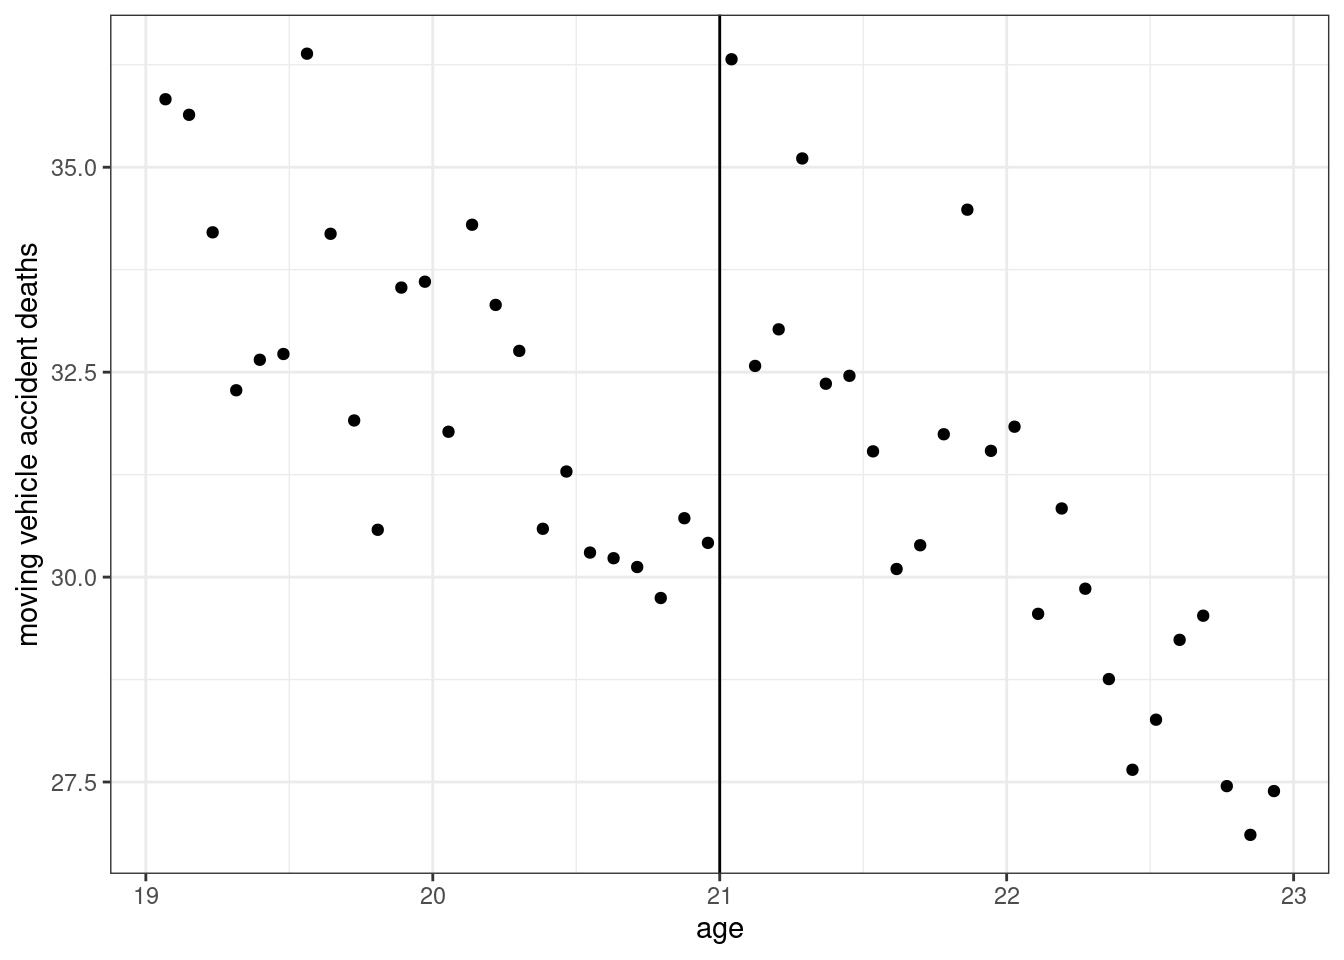
\includegraphics{17-quasi_experiments_files/figure-pdf/unnamed-chunk-7-1.pdf}

This figure at least suggests that the number of car accident deaths
does appear to jump at age 21.

Now, let's run the regression that we talked about earlier, involving a
treatment dummy, age, and age interacted with the treatment.

\begin{Shaded}
\begin{Highlighting}[]
\NormalTok{rd\_reg }\OtherTok{\textless{}{-}} \FunctionTok{lm}\NormalTok{(mva }\SpecialCharTok{\textasciitilde{}}\NormalTok{ D }\SpecialCharTok{+}\NormalTok{ agecell }\SpecialCharTok{+}\NormalTok{ agecell}\SpecialCharTok{*}\NormalTok{D, }\AttributeTok{data=}\NormalTok{mlda)}
\FunctionTok{summary}\NormalTok{(rd\_reg)}
\end{Highlighting}
\end{Shaded}

\begin{verbatim}

Call:
lm(formula = mva ~ D + agecell + agecell * D, data = mlda)

Residuals:
    Min      1Q  Median      3Q     Max 
-2.4124 -0.7774 -0.2913  0.8495  3.2378 

Coefficients:
            Estimate Std. Error t value Pr(>|t|)    
(Intercept)  83.8492     9.3328   8.984 1.63e-11 ***
D            28.9450    13.8638   2.088   0.0426 *  
agecell      -2.5676     0.4661  -5.508 1.77e-06 ***
D:agecell    -1.1624     0.6592  -1.763   0.0848 .  
---
Signif. codes:  0 '***' 0.001 '**' 0.01 '*' 0.05 '.' 0.1 ' ' 1

Residual standard error: 1.299 on 44 degrees of freedom
Multiple R-squared:  0.7222,    Adjusted R-squared:  0.7032 
F-statistic: 38.13 on 3 and 44 DF,  p-value: 2.671e-12
\end{verbatim}

These results suggest that alcohol consumption increased car accident
deaths (you can see this from the estimated coefficient on \texttt{D}).
{[}The setup in this example is somewhat simplified; if you wanted to be
careful about how much alcohol consumption increased car accident
deaths, then we would probably need to scale up our estimate by how much
alcohol consumption increases on average when people turn 21.
Nevertheless, what we have presented above does suggest that alcohol
consumption increases car accident deaths.{]}

Finally, let me show one more plot that is common to report in a
regression discontinuity design.

\begin{Shaded}
\begin{Highlighting}[]
\CommentTok{\# get predicted values for plotting}
\NormalTok{mlda}\SpecialCharTok{$}\NormalTok{preds }\OtherTok{\textless{}{-}} \FunctionTok{predict}\NormalTok{(rd\_reg)}

\CommentTok{\# make plot}
\FunctionTok{ggplot}\NormalTok{(mlda, }\FunctionTok{aes}\NormalTok{(}\AttributeTok{x=}\NormalTok{agecell, }\AttributeTok{y=}\NormalTok{mva, }\AttributeTok{color=}\FunctionTok{as.factor}\NormalTok{(D))) }\SpecialCharTok{+}
  \FunctionTok{geom\_point}\NormalTok{() }\SpecialCharTok{+}
  \FunctionTok{geom\_line}\NormalTok{(}\FunctionTok{aes}\NormalTok{(}\AttributeTok{y=}\NormalTok{preds)) }\SpecialCharTok{+} 
  \FunctionTok{geom\_vline}\NormalTok{(}\AttributeTok{xintercept=}\DecValTok{21}\NormalTok{) }\SpecialCharTok{+}
  \FunctionTok{labs}\NormalTok{(}\AttributeTok{color=}\StringTok{"treated"}\NormalTok{, }\AttributeTok{x=}\StringTok{"age"}\NormalTok{, }\AttributeTok{y=}\StringTok{"moving vehicle accident deaths"}\NormalTok{) }\SpecialCharTok{+} 
  \FunctionTok{theme\_bw}\NormalTok{()}
\end{Highlighting}
\end{Shaded}

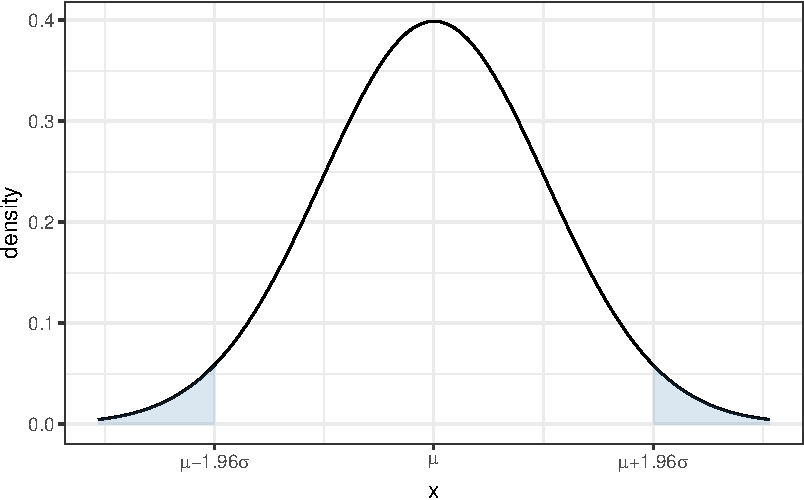
\includegraphics{17-quasi_experiments_files/figure-pdf/unnamed-chunk-9-1.pdf}

This shows the two lines that we effectively fit with the regression
that included the binary variable for the treatment, the running
variable, and their interaction. The ``jump'' between the red line and
the blue line at \texttt{age=21} is our estimated effect of the
treatment.

\section{Lab 7: Drunk Driving Laws}\label{lab-7-drunk-driving-laws}

For this lab, we will use the \texttt{Fatalities} data. We will study
the causal effect of mandatory jail sentence policies for drunk driving
on traffic fatalities. The \texttt{Fatalities} data consists of panel
data of traffic fatality death rates, whether or not a state has a
mandatory jail sentence policy or not as well as several other variables
from 1982-1988. Economic theory suggests that raising the cost of some
behavior (in this case, you can think of a mandatory jail sentence as
raising the cost of drunk driving) will lead to less of that behavior.
That being said, it's both interesting to test this theory and also
consider the magnitude of this effect. That's what we'll do in this
problem.

\begin{enumerate}
\def\labelenumi{\arabic{enumi}.}
\item
  This data comes in a somewhat messier format than some of the data
  that we have used previously. To start with, create a new column in
  the data called \texttt{afatal\_per\_million} that is the number of
  alcohol involved vehicle fatalities per millions people in a state in
  a particular year. The variable \texttt{afatal} contains the total
  number of alcohol involved vehicle fatalities, and the variable
  \texttt{pop} contains the total population in a state.
\item
  Using a subset of the data from 1988, run a regression of
  \texttt{afatal\_per\_million} on whether or not a state has a
  mandatory jail sentence policy \texttt{jail}. How do you interpret the
  results?
\item
  Using the same subset from part 2, run a regression of
  \texttt{afatal\_per\_million} on \texttt{jail}, unemployment rate
  (\texttt{unemp}), the tax on a case of beer (\texttt{beertax}), the
  percentage of southern baptists in the state (\texttt{baptist}), the
  percentage of residents residing in dry counties (\texttt{dry}), the
  percentage of young drivers in the state, (\texttt{youngdrivers}), and
  the average miles driven per person in a state (\texttt{miles}). How
  do you interpret the estimated coefficient on \texttt{jail}? Would you
  consider this to be a reasonable estimate of the (average) causal
  effect of mandatory jail policies on alcohol related fatalities?
\item
  Now, using the full data, let's estimate a fixed effects model with
  alcohol related fatalities per million as the outcome and mandatory
  jail policies as a regressor. Estimate the model using first
  differences and make sure to include time fixed effects. How do you
  interpret the results?
\item
  Estimate the same model as in part 4, but using the within estimator
  instead of first differences. Compare these results to the ones from
  part 4.
\item
  Using the same within estimator as in part 5, include the same set of
  covariates from part 3 and interpret the estimated effect of mandatory
  jail policies. How do these estimates compare to the earlier ones?
\item
  Now, we'll switch to using a difference in differences approach to
  estimating the effect of mandatory jail policies. First, we'll
  manipulate the data some.

  \begin{enumerate}
  \def\labelenumii{\alph{enumii})}
  \item
    To keep things simple, let's start by limiting the data to the years
    1982 and 1988 and drop the in-between periods.
  \item
    Second, let's calculate the change in alcohol related fatalities per
    million between 1982 and 1998 and keep the covariates that we have
    been using from 1982. One way to do this, is to use the
    \texttt{pivot\_wider} function from the \texttt{tidyr}. In the case
    of panel data, ``long format'' data means that each row in the data
    corresponds to a paricular observation \emph{and} a particular time
    period. Thus, with long format data, there are \(n \times T\) total
    rows in the data. On the other hand, ``wide format'' data means that
    each row holds all the data (across all time periods) for a
    particular observation. Converting back and forth between long and
    wide formats is a common data manipulation task. \textbf{Hint:} This
    step is probably unfamiliar, so I'd recommend seeing if you can use
    \texttt{?tidyr::pivot\_wider} to see if you can figure out how to
    complete this step, but, if not, you can copy this code from the
    solutions in the next section.
  \item
    Finally, drop all states that are already treated in 1982.
  \end{enumerate}
\item
  Using the data that you constructed in part 7, implement the
  difference in differences regression of the change in alcohol related
  fatalities per million from 1982 to 1988 on the mandatory jail policy.
  How do you interpret these results and how do they compare to the
  previous ones? Now, additionally include the set of covariates that we
  have been using in this model. How do you interpret these results and
  how do they compare to the previous ones?
\item
  An alternative to DID, is to include the lagged outcome as a
  covariate. Using the data constructed in part 7, run a regression of
  alcohol related fatalities per million in 1988 on the mandatory jail
  policy and alcohol related fatalities per million in 1982. How do you
  interpret these results and how do they compare to the previous ones?
  Now include the additional covariates that we have been using in this
  model. How do you interpret these results and how do they compare to
  the previous ones?
\item
  Comment on your results from parts 1-9. Which, if any, of these are
  you most inclined to interpret as a reasonable estimate of the
  (average) causal effect of mandatory jail policies on alcohol related
  policies?
\end{enumerate}

\section{Lab 7: Solutions}\label{lab-7-solutions}

\begin{enumerate}
\def\labelenumi{\arabic{enumi}.}
\tightlist
\item
\end{enumerate}

\begin{Shaded}
\begin{Highlighting}[]
\FunctionTok{library}\NormalTok{(tidyr)}
\FunctionTok{library}\NormalTok{(plm)}

\FunctionTok{data}\NormalTok{(Fatalities, }\AttributeTok{package=}\StringTok{"AER"}\NormalTok{)}

\NormalTok{Fatalities}\SpecialCharTok{$}\NormalTok{afatal\_per\_million }\OtherTok{\textless{}{-}} \DecValTok{1000000} \SpecialCharTok{*}\NormalTok{ (Fatalities}\SpecialCharTok{$}\NormalTok{afatal }\SpecialCharTok{/}\NormalTok{ Fatalities}\SpecialCharTok{$}\NormalTok{pop )}
\end{Highlighting}
\end{Shaded}

\begin{enumerate}
\def\labelenumi{\arabic{enumi}.}
\setcounter{enumi}{1}
\tightlist
\item
\end{enumerate}

\begin{Shaded}
\begin{Highlighting}[]
\NormalTok{Fatalities88 }\OtherTok{\textless{}{-}} \FunctionTok{subset}\NormalTok{(Fatalities, year}\SpecialCharTok{==}\DecValTok{1988}\NormalTok{)}

\NormalTok{reg88 }\OtherTok{\textless{}{-}} \FunctionTok{lm}\NormalTok{(afatal\_per\_million }\SpecialCharTok{\textasciitilde{}}\NormalTok{ jail, }\AttributeTok{data=}\NormalTok{Fatalities88)}
\FunctionTok{summary}\NormalTok{(reg88)}
\end{Highlighting}
\end{Shaded}

\begin{verbatim}

Call:
lm(formula = afatal_per_million ~ jail, data = Fatalities88)

Residuals:
    Min      1Q  Median      3Q     Max 
-36.123 -16.622  -1.469   8.642 112.260 

Coefficients:
            Estimate Std. Error t value Pr(>|t|)    
(Intercept)   59.496      4.273  13.923   <2e-16 ***
jailyes        9.155      7.829   1.169    0.248    
---
Signif. codes:  0 '***' 0.001 '**' 0.01 '*' 0.05 '.' 0.1 ' ' 1

Residual standard error: 24.55 on 45 degrees of freedom
  (1 observation deleted due to missingness)
Multiple R-squared:  0.02949,   Adjusted R-squared:  0.007921 
F-statistic: 1.367 on 1 and 45 DF,  p-value: 0.2484
\end{verbatim}

The estimated coefficient on mandatory jail laws is 9.155. We should
interpret this as just the difference between alcohol related fatalities
per million in states that had mandatory jail laws in 1988 relative to
states that did not have them. We cannot reject that there is no
difference between states where the policy is in place relative to those
that do not have the policy.

\begin{enumerate}
\def\labelenumi{\arabic{enumi}.}
\setcounter{enumi}{2}
\tightlist
\item
\end{enumerate}

\begin{Shaded}
\begin{Highlighting}[]
\NormalTok{reg88\_covs }\OtherTok{\textless{}{-}} \FunctionTok{lm}\NormalTok{(afatal\_per\_million }\SpecialCharTok{\textasciitilde{}}\NormalTok{ jail }\SpecialCharTok{+}\NormalTok{ unemp }\SpecialCharTok{+}\NormalTok{ beertax }\SpecialCharTok{+}\NormalTok{ baptist }\SpecialCharTok{+}\NormalTok{ dry }\SpecialCharTok{+}\NormalTok{ youngdrivers }\SpecialCharTok{+}\NormalTok{ miles, }\AttributeTok{data=}\NormalTok{Fatalities88)}
\FunctionTok{summary}\NormalTok{(reg88\_covs)}
\end{Highlighting}
\end{Shaded}

\begin{verbatim}

Call:
lm(formula = afatal_per_million ~ jail + unemp + beertax + baptist + 
    dry + youngdrivers + miles, data = Fatalities88)

Residuals:
    Min      1Q  Median      3Q     Max 
-39.065  -9.907  -1.690   9.673  82.100 

Coefficients:
               Estimate Std. Error t value Pr(>|t|)  
(Intercept)  -29.373536  32.500240  -0.904   0.3717  
jailyes        3.120574   6.849271   0.456   0.6512  
unemp          4.815081   1.892369   2.544   0.0150 *
beertax        2.311850   9.521684   0.243   0.8094  
baptist        0.661694   0.527228   1.255   0.2169  
dry           -0.026675   0.383956  -0.069   0.9450  
youngdrivers  -0.092100 142.804244  -0.001   0.9995  
miles          0.006802   0.002822   2.411   0.0207 *
---
Signif. codes:  0 '***' 0.001 '**' 0.01 '*' 0.05 '.' 0.1 ' ' 1

Residual standard error: 19.41 on 39 degrees of freedom
  (1 observation deleted due to missingness)
Multiple R-squared:  0.4742,    Adjusted R-squared:  0.3798 
F-statistic: 5.024 on 7 and 39 DF,  p-value: 0.0003999
\end{verbatim}

The estimated coefficient on jail is 3.12. It is somewhat smaller than
the previous estimate, though neither is statistically significant. We
should interpret this as the partial effect of the mandatory jail
policy, that is, that we estimate that mandatory jail laws increase the
number of alcohol related fatalities per million by 3.12 on average
controlling for the unemployment rate, beer tax, the fraction of
southern baptists in the state, the fraction of residents in dry
counties, the fraction of young drivers, and the average miles driven in
the state. We cannot reject that the partial effect of mandatory jail
policies is equal to 0.

\begin{enumerate}
\def\labelenumi{\arabic{enumi}.}
\setcounter{enumi}{3}
\tightlist
\item
\end{enumerate}

\begin{Shaded}
\begin{Highlighting}[]
\NormalTok{fd\_reg }\OtherTok{\textless{}{-}} \FunctionTok{plm}\NormalTok{(afatal\_per\_million }\SpecialCharTok{\textasciitilde{}}\NormalTok{ jail }\SpecialCharTok{+} \FunctionTok{as.factor}\NormalTok{(year),}
              \AttributeTok{effect=}\StringTok{"individual"}\NormalTok{,}
              \AttributeTok{index=}\StringTok{"state"}\NormalTok{, }\AttributeTok{model=}\StringTok{"fd"}\NormalTok{,}
              \AttributeTok{data=}\NormalTok{Fatalities)}
\FunctionTok{summary}\NormalTok{(fd\_reg)}
\end{Highlighting}
\end{Shaded}

\begin{verbatim}
Oneway (individual) effect First-Difference Model

Call:
plm(formula = afatal_per_million ~ jail + as.factor(year), data = Fatalities, 
    effect = "individual", model = "fd", index = "state")

Unbalanced Panel: n = 48, T = 6-7, N = 335
Observations used in estimation: 287

Residuals:
     Min.   1st Qu.    Median   3rd Qu.      Max. 
-51.66677  -5.09887   0.23801   6.28688 119.08976 

Coefficients: (1 dropped because of singularities)
                    Estimate Std. Error t-value Pr(>|t|)   
(Intercept)         -2.15376    0.80673 -2.6697 0.008035 **
jailyes              2.60763    5.28351  0.4935 0.622016   
as.factor(year)1983 -5.28423    1.82330 -2.8982 0.004050 **
as.factor(year)1984 -3.58247    2.29451 -1.5613 0.119577   
as.factor(year)1985 -5.60800    2.43517 -2.3029 0.022017 * 
as.factor(year)1986 -0.74192    2.28988 -0.3240 0.746180   
as.factor(year)1987 -2.16244    1.80716 -1.1966 0.232476   
---
Signif. codes:  0 '***' 0.001 '**' 0.01 '*' 0.05 '.' 0.1 ' ' 1

Total Sum of Squares:    54692
Residual Sum of Squares: 51620
R-Squared:      0.056171
Adj. R-Squared: 0.035946
F-statistic: 2.77733 on 6 and 280 DF, p-value: 0.012223
\end{verbatim}

We should interpret the estimated coefficient on \texttt{jail} as an
estimate of how much alcohol related traffic fatalities per million
change on average under mandatory jail policies after accounting for
time invariant variables whose effects do not change over time. Again,
we cannot reject that the effect is equal to 0.

\begin{enumerate}
\def\labelenumi{\arabic{enumi}.}
\setcounter{enumi}{4}
\tightlist
\item
\end{enumerate}

\begin{Shaded}
\begin{Highlighting}[]
\NormalTok{within\_reg }\OtherTok{\textless{}{-}} \FunctionTok{plm}\NormalTok{(afatal\_per\_million }\SpecialCharTok{\textasciitilde{}}\NormalTok{ jail }\SpecialCharTok{+} \FunctionTok{as.factor}\NormalTok{(year),}
              \AttributeTok{effect=}\StringTok{"individual"}\NormalTok{,}
              \AttributeTok{index=}\StringTok{"state"}\NormalTok{, }\AttributeTok{model=}\StringTok{"within"}\NormalTok{,}
              \AttributeTok{data=}\NormalTok{Fatalities)}
\FunctionTok{summary}\NormalTok{(within\_reg)}
\end{Highlighting}
\end{Shaded}

\begin{verbatim}
Oneway (individual) effect Within Model

Call:
plm(formula = afatal_per_million ~ jail + as.factor(year), data = Fatalities, 
    effect = "individual", model = "within", index = "state")

Unbalanced Panel: n = 48, T = 6-7, N = 335

Residuals:
       Min.     1st Qu.      Median     3rd Qu.        Max. 
-95.1937300  -4.9678238   0.0088078   5.1611249  40.6263546 

Coefficients:
                    Estimate Std. Error t-value  Pr(>|t|)    
jailyes               8.3327     4.9666  1.6777 0.0945164 .  
as.factor(year)1983  -7.9151     2.6936 -2.9384 0.0035734 ** 
as.factor(year)1984  -8.4863     2.7115 -3.1298 0.0019341 ** 
as.factor(year)1985 -12.7849     2.7331 -4.6778 4.518e-06 ***
as.factor(year)1986 -10.0726     2.7331 -3.6854 0.0002741 ***
as.factor(year)1987 -13.5276     2.7115 -4.9890 1.067e-06 ***
as.factor(year)1988 -13.6296     2.7279 -4.9964 1.030e-06 ***
---
Signif. codes:  0 '***' 0.001 '**' 0.01 '*' 0.05 '.' 0.1 ' ' 1

Total Sum of Squares:    53854
Residual Sum of Squares: 47607
R-Squared:      0.116
Adj. R-Squared: -0.054487
F-statistic: 5.24882 on 7 and 280 DF, p-value: 1.2051e-05
\end{verbatim}

The estimated coefficient on \texttt{jail} has the same interpretation
as in the previous problem. The estimated effect here is marginally
statistically significant. 6.

\begin{Shaded}
\begin{Highlighting}[]
\NormalTok{within\_reg\_covs }\OtherTok{\textless{}{-}} \FunctionTok{plm}\NormalTok{(afatal\_per\_million }\SpecialCharTok{\textasciitilde{}}\NormalTok{ jail }\SpecialCharTok{+}\NormalTok{ unemp }\SpecialCharTok{+}\NormalTok{ beertax }\SpecialCharTok{+}\NormalTok{ baptist }\SpecialCharTok{+}\NormalTok{ dry }\SpecialCharTok{+}\NormalTok{ youngdrivers }\SpecialCharTok{+}\NormalTok{ miles,}
                       \AttributeTok{effect=}\StringTok{"individual"}\NormalTok{,}
                       \AttributeTok{index=}\StringTok{"state"}\NormalTok{, }\AttributeTok{model=}\StringTok{"within"}\NormalTok{,}
                       \AttributeTok{data=}\NormalTok{Fatalities)}
\FunctionTok{summary}\NormalTok{(within\_reg\_covs)}
\end{Highlighting}
\end{Shaded}

\begin{verbatim}
Oneway (individual) effect Within Model

Call:
plm(formula = afatal_per_million ~ jail + unemp + beertax + baptist + 
    dry + youngdrivers + miles, data = Fatalities, effect = "individual", 
    model = "within", index = "state")

Unbalanced Panel: n = 48, T = 6-7, N = 335

Residuals:
     Min.   1st Qu.    Median   3rd Qu.      Max. 
-95.62306  -5.69773  -0.56903   4.79219  47.80871 

Coefficients:
                Estimate  Std. Error t-value  Pr(>|t|)    
jailyes       4.9731e+00  4.9613e+00  1.0024   0.31702    
unemp        -1.1340e+00  5.6592e-01 -2.0038   0.04605 *  
beertax      -2.7456e+01  1.5080e+01 -1.8207   0.06972 .  
baptist       2.5083e+00  4.3324e+00  0.5790   0.56308    
dry           4.3092e-01  1.0870e+00  0.3964   0.69208    
youngdrivers  2.6357e+02  5.0169e+01  5.2537 2.957e-07 ***
miles        -6.8899e-04  7.3182e-04 -0.9415   0.34727    
---
Signif. codes:  0 '***' 0.001 '**' 0.01 '*' 0.05 '.' 0.1 ' ' 1

Total Sum of Squares:    53854
Residual Sum of Squares: 48083
R-Squared:      0.10717
Adj. R-Squared: -0.065023
F-statistic: 4.80119 on 7 and 280 DF, p-value: 4.0281e-05
\end{verbatim}

We should interpret the estimated coefficient on \texttt{jail} as an
estimate of how much alcohol related traffic fatalities per million
change on average under mandatory jail policies after controlling for
the unemployment rate, beer taxes, the fraction of the state that is
southern baptist, the fraction of the state that lives in a dry county,
the fraction of young drivers in a state, and the average number of
miles driven per person in the stata, and accounting for time invariant
variables whose effects do not change over time.

\begin{enumerate}
\def\labelenumi{\arabic{enumi}.}
\setcounter{enumi}{6}
\tightlist
\item
\end{enumerate}

\begin{Shaded}
\begin{Highlighting}[]
\CommentTok{\# part a: convert data to two period panel data}
\NormalTok{two\_period }\OtherTok{\textless{}{-}} \FunctionTok{subset}\NormalTok{(Fatalities, year}\SpecialCharTok{==}\DecValTok{1982} \SpecialCharTok{|}\NormalTok{ year}\SpecialCharTok{==}\DecValTok{1988}\NormalTok{)}
\CommentTok{\# and drop some missing}
\NormalTok{two\_period }\OtherTok{\textless{}{-}} \FunctionTok{subset}\NormalTok{(two\_period, }\SpecialCharTok{!}\FunctionTok{is.na}\NormalTok{(jail))}
\NormalTok{two\_period }\OtherTok{\textless{}{-}}\NormalTok{ BMisc}\SpecialCharTok{::}\FunctionTok{makeBalancedPanel}\NormalTok{(two\_period, }\StringTok{"state"}\NormalTok{, }\StringTok{"year"}\NormalTok{)}
\NormalTok{two\_period}\SpecialCharTok{$}\NormalTok{jail }\OtherTok{\textless{}{-}} \DecValTok{1}\SpecialCharTok{*}\NormalTok{(two\_period}\SpecialCharTok{$}\NormalTok{jail}\SpecialCharTok{==}\StringTok{"yes"}\NormalTok{)}

\CommentTok{\# part b: convert into wide format}
\NormalTok{wide\_df }\OtherTok{\textless{}{-}} \FunctionTok{pivot\_wider}\NormalTok{(two\_period, }
                       \AttributeTok{id\_cols=}\StringTok{"state"}\NormalTok{, }
                       \AttributeTok{names\_from=}\StringTok{"year"}\NormalTok{,}
                       \AttributeTok{values\_from=}\FunctionTok{c}\NormalTok{(}\StringTok{"jail"}\NormalTok{, }\StringTok{"afatal\_per\_million"}\NormalTok{))}

\CommentTok{\# add back other covariates from 1982}
\NormalTok{wide\_df }\OtherTok{\textless{}{-}} \FunctionTok{merge}\NormalTok{(wide\_df, }\FunctionTok{subset}\NormalTok{(Fatalities, year}\SpecialCharTok{==}\DecValTok{1982}\NormalTok{)[,}\FunctionTok{c}\NormalTok{(}\StringTok{"unemp"}\NormalTok{, }\StringTok{"beertax"}\NormalTok{, }\StringTok{"baptist"}\NormalTok{, }\StringTok{"dry"}\NormalTok{, }\StringTok{"youngdrivers"}\NormalTok{, }\StringTok{"miles"}\NormalTok{,}\StringTok{"state"}\NormalTok{)], }\AttributeTok{by=}\StringTok{"state"}\NormalTok{)}

\CommentTok{\# change in fatal accidents over time}
\NormalTok{wide\_df}\SpecialCharTok{$}\NormalTok{Dafatal\_per\_million }\OtherTok{\textless{}{-}}\NormalTok{ wide\_df}\SpecialCharTok{$}\NormalTok{afatal\_per\_million\_1988 }\SpecialCharTok{{-}}\NormalTok{ wide\_df}\SpecialCharTok{$}\NormalTok{afatal\_per\_million\_1982}

\CommentTok{\# part c: drop already treated states}
\NormalTok{wide\_df }\OtherTok{\textless{}{-}} \FunctionTok{subset}\NormalTok{(wide\_df, jail\_1982}\SpecialCharTok{==}\DecValTok{0}\NormalTok{)}
\end{Highlighting}
\end{Shaded}

\begin{enumerate}
\def\labelenumi{\arabic{enumi}.}
\setcounter{enumi}{7}
\tightlist
\item
\end{enumerate}

\begin{Shaded}
\begin{Highlighting}[]
\NormalTok{did }\OtherTok{\textless{}{-}} \FunctionTok{lm}\NormalTok{(Dafatal\_per\_million }\SpecialCharTok{\textasciitilde{}}\NormalTok{ jail\_1988, }\AttributeTok{data=}\NormalTok{wide\_df)}
\FunctionTok{summary}\NormalTok{(did)}
\end{Highlighting}
\end{Shaded}

\begin{verbatim}

Call:
lm(formula = Dafatal_per_million ~ jail_1988, data = wide_df)

Residuals:
    Min      1Q  Median      3Q     Max 
-55.652 -10.993   5.033  10.405  76.822 

Coefficients:
            Estimate Std. Error t value Pr(>|t|)   
(Intercept)  -12.585      4.242  -2.966  0.00532 **
jail_1988      5.102     11.695   0.436  0.66526   
---
Signif. codes:  0 '***' 0.001 '**' 0.01 '*' 0.05 '.' 0.1 ' ' 1

Residual standard error: 24.37 on 36 degrees of freedom
Multiple R-squared:  0.005259,  Adjusted R-squared:  -0.02237 
F-statistic: 0.1903 on 1 and 36 DF,  p-value: 0.6653
\end{verbatim}

\begin{Shaded}
\begin{Highlighting}[]
\NormalTok{did\_covs }\OtherTok{\textless{}{-}} \FunctionTok{lm}\NormalTok{(Dafatal\_per\_million }\SpecialCharTok{\textasciitilde{}}\NormalTok{ jail\_1988 }\SpecialCharTok{+}\NormalTok{ unemp }\SpecialCharTok{+}\NormalTok{ beertax }\SpecialCharTok{+}\NormalTok{ baptist }\SpecialCharTok{+}\NormalTok{ dry }\SpecialCharTok{+}\NormalTok{ youngdrivers }\SpecialCharTok{+}\NormalTok{ miles, }\AttributeTok{data=}\NormalTok{wide\_df)}
\FunctionTok{summary}\NormalTok{(did\_covs)}
\end{Highlighting}
\end{Shaded}

\begin{verbatim}

Call:
lm(formula = Dafatal_per_million ~ jail_1988 + unemp + beertax + 
    baptist + dry + youngdrivers + miles, data = wide_df)

Residuals:
    Min      1Q  Median      3Q     Max 
-38.346 -12.383   1.456   9.092  60.585 

Coefficients:
               Estimate Std. Error t value Pr(>|t|)  
(Intercept)    6.851636  50.643035   0.135   0.8933  
jail_1988     -1.853041  10.834391  -0.171   0.8653  
unemp          3.725007   1.919862   1.940   0.0618 .
beertax        8.300778  10.052007   0.826   0.4154  
baptist        0.527893   0.723263   0.730   0.4711  
dry           -0.955636   0.546475  -1.749   0.0906 .
youngdrivers  89.432017 234.379768   0.382   0.7055  
miles         -0.010360   0.005823  -1.779   0.0854 .
---
Signif. codes:  0 '***' 0.001 '**' 0.01 '*' 0.05 '.' 0.1 ' ' 1

Residual standard error: 21.9 on 30 degrees of freedom
Multiple R-squared:  0.3303,    Adjusted R-squared:  0.174 
F-statistic: 2.114 on 7 and 30 DF,  p-value: 0.07276
\end{verbatim}

If we are willing to believe that, in the absence of the policy, that
trends in alcohol related fatalities per million people would have
followed the same trends over time for treated and untreated states,
then we can interpret these as causal effects. These estimates are
broadly similar to the previous ones though the second ones (that
include additional covariates) are about the only ones where we ever get
a negative estimate for the effect of mandatory jail policies. Like the
previous estimates, neither of these estimates are statistically
different from 0.

\begin{enumerate}
\def\labelenumi{\arabic{enumi}.}
\setcounter{enumi}{8}
\tightlist
\item
\end{enumerate}

\begin{Shaded}
\begin{Highlighting}[]
\NormalTok{lag\_reg }\OtherTok{\textless{}{-}} \FunctionTok{lm}\NormalTok{(afatal\_per\_million\_1988 }\SpecialCharTok{\textasciitilde{}}\NormalTok{ jail\_1988 }\SpecialCharTok{+}\NormalTok{ afatal\_per\_million\_1982, }\AttributeTok{data=}\NormalTok{wide\_df)}
\FunctionTok{summary}\NormalTok{(lag\_reg)}
\end{Highlighting}
\end{Shaded}

\begin{verbatim}

Call:
lm(formula = afatal_per_million_1988 ~ jail_1988 + afatal_per_million_1982, 
    data = wide_df)

Residuals:
    Min      1Q  Median      3Q     Max 
-29.120 -12.663  -0.684   6.873  92.390 

Coefficients:
                        Estimate Std. Error t value Pr(>|t|)    
(Intercept)              19.0810    10.1089   1.888 0.067401 .  
jail_1988                 3.4323    10.3171   0.333 0.741363    
afatal_per_million_1982   0.5607     0.1303   4.303 0.000129 ***
---
Signif. codes:  0 '***' 0.001 '**' 0.01 '*' 0.05 '.' 0.1 ' ' 1

Residual standard error: 21.47 on 35 degrees of freedom
Multiple R-squared:  0.3462,    Adjusted R-squared:  0.3088 
F-statistic: 9.266 on 2 and 35 DF,  p-value: 0.0005896
\end{verbatim}

\begin{Shaded}
\begin{Highlighting}[]
\NormalTok{lag\_reg\_covs }\OtherTok{\textless{}{-}} \FunctionTok{lm}\NormalTok{(afatal\_per\_million\_1988 }\SpecialCharTok{\textasciitilde{}}\NormalTok{ jail\_1988 }\SpecialCharTok{+}\NormalTok{ afatal\_per\_million\_1982 }\SpecialCharTok{+}\NormalTok{ unemp }\SpecialCharTok{+}\NormalTok{ beertax }\SpecialCharTok{+}\NormalTok{ baptist }\SpecialCharTok{+}\NormalTok{ dry }\SpecialCharTok{+}\NormalTok{ youngdrivers }\SpecialCharTok{+}\NormalTok{ miles, }\AttributeTok{data=}\NormalTok{wide\_df)}
\FunctionTok{summary}\NormalTok{(lag\_reg\_covs)}
\end{Highlighting}
\end{Shaded}

\begin{verbatim}

Call:
lm(formula = afatal_per_million_1988 ~ jail_1988 + afatal_per_million_1982 + 
    unemp + beertax + baptist + dry + youngdrivers + miles, data = wide_df)

Residuals:
    Min      1Q  Median      3Q     Max 
-27.840  -8.793  -1.364   5.146  71.409 

Coefficients:
                          Estimate Std. Error t value Pr(>|t|)   
(Intercept)             -17.292595  46.318477  -0.373  0.71161   
jail_1988                 0.817453   9.786782   0.084  0.93401   
afatal_per_million_1982   0.505371   0.173718   2.909  0.00689 **
unemp                     3.189918   1.736443   1.837  0.07647 . 
beertax                   2.885796   9.236174   0.312  0.75694   
baptist                   0.965785   0.668259   1.445  0.15911   
dry                      -0.567567   0.509915  -1.113  0.27482   
youngdrivers            120.615853 211.026841   0.572  0.57202   
miles                    -0.002692   0.005888  -0.457  0.65087   
---
Signif. codes:  0 '***' 0.001 '**' 0.01 '*' 0.05 '.' 0.1 ' ' 1

Residual standard error: 19.7 on 29 degrees of freedom
Multiple R-squared:  0.5443,    Adjusted R-squared:  0.4186 
F-statistic: 4.329 on 8 and 29 DF,  p-value: 0.001596
\end{verbatim}

These estimates directly control for alcohol related fatalities per
million in the pre-treatment period 1982. These sorts of specifications
are less common in economics, but, in my view, it seems like a
reasonable approach here. That said, the results are more or less the
same as earlier estimates.

\begin{enumerate}
\def\labelenumi{\arabic{enumi}.}
\setcounter{enumi}{9}
\tightlist
\item
  We don't have very strong evidence that mandatory jail policies
  reduced the number traffic fatalities. In my view, probably the best
  specifications for trying to understand the causal effects are the
  ones in part 7 (particularly, the ones that include covariates there),
  but I think that the the results in parts 4-9 are also informative.
  Broadly, these estimates are more or less similar --- none of them are
  statistically significant and most are positive (which is an
  unexpected sign).
\end{enumerate}

Before we finish, let me mention a few caveats to these results:

\begin{itemize}
\item
  First, I would be very hesitant to interpret these results as
  definitively saying that mandatory jail policies have no effect on
  alcohol related traffic fatalities. The main reason to be clear about
  this is that our standard error are quite large. For example, in the
  second specification in part 7 (the one I like the most), a 95\%
  confidence interval for our estimate is \([-23.1, 19.4]\). This is a
  wide confidence interval --- the average number of alcohol related
  traffic fatalities per million across all states and time periods is
  only 66. So our estimates are basically still compatible with very
  large reductions in alcohol related traffic fatalities up to large
  increases in alcohol related traffic fatalities.
\item
  Let me make one more comment about the sign of our results. Many of
  our point estimates are positive; as we discussed earlier, it is hard
  to rationalize harsher punishments \emph{increasing} alcohol related
  traffic fatalities. I think the main explanation for these results is
  just that our estimates are pretty noisy and, therefore, more or less
  ``by chance'' we are getting estimates that have an unexpected sign.
  But there are some other possible explanations that are worth
  mentioning. For one, there are a number of other policies related to
  drunk driving that occurred in the 1980s (particularly, related to
  legal drinking age) but perhaps others. It is not clear how these
  would interact with our estimates, but they could certainly play some
  role. Besides that, it seems to me that we have a pretty good set of
  covariates that enter our models, but there could be important
  covariates that we are missing. For this reason, some expertise in how
  to model state-level traffic fatalities is actually a very important
  skill here (actually probably the key skill here!)
\end{itemize}

\section{Coding Questions}\label{coding-questions-4}

\begin{enumerate}
\def\labelenumi{\arabic{enumi}.}
\item
  For this problem, we will use the data \texttt{rand\_hie}. This is
  data from the RAND health insurance experiment in the 1980s. In the
  experiment, participants were randomly assigned to get Catastrophic
  (the least amount of coverage), insurance that came with a Deductible,
  insurance that came with Cost Sharing (i.e., co-insurance so that an
  individual pays part of their medical insurance), and Free (so that
  there is no cost of medical care).

  For this problem, we will be interested in whether or not changing the
  type of health insurance changed the amount of health care utilization
  and the health status of individuals.

  We will focus on the difference between the least amount of health
  insurance (``Catastrophic'') and the most amount of health insurance
  (``Free''). In particular, you can start this problem by creating a
  new dataset by running the following command:
  \texttt{rand\_hie\_subset\ \textless{}-\ subset(rand\_hie,\ plan\_type\ \%in\%\ c("Catastrophic",\ "Free"))}

  and use this data to answer the questions below.

  \begin{enumerate}
  \def\labelenumii{\alph{enumii})}
  \item
    Use a regression to estimate the average difference between total
    medical expenditure (\texttt{total\_med\_expenditure}) by plan type
    (\texttt{plan\_type}) and report your results. Should you interpret
    these as average causal effects? Explain.
  \item
    Use a regression to estimate the average difference between face to
    face doctors visits (\texttt{face\_to\_face\_visits}) by plan type
    (\texttt{plan\_type}) and report your results. Should you interpret
    these as average causal effects? Explain.
  \item
    Use a regression to estimate the average difference between the
    overall health index (\texttt{health\_index}) by plan type
    (\texttt{plan\_type}) and report your results. Should you interpret
    these as average causal effects? Explain.
  \item
    How do you interpret the results from parts a-c?
  \end{enumerate}
\item
  For this problem, we will study the causal effect of having more
  children on women's labor supply using the data \texttt{Fertility}.

  \begin{enumerate}
  \def\labelenumii{\alph{enumii})}
  \item
    Let's start by running a regression of the number of hours that a
    woman typically works per week (\texttt{work}) on whether or not she
    has more than two children (\texttt{morekids}), her age and
    \(age^2\), and race/ethnicity (\texttt{afam} and \texttt{hispanic}).
    Report your results. How do you feel about interpreting the
    estimated coefficient on \texttt{morekids} as the causal effect of
    having more than two children? Explain.
  \item
    One possible instrument in this setup is the sex composition of the
    first two children (i.e., whether they are both girls, both boys, or
    a boy and a girl). The thinking here is that, at least in the United
    States, parents tend to have a preference for having both a girl and
    a boy and that, therefore, parents whose first two children have the
    same sex may be more likely to have a third child than they would
    have been if they have a girl and a boy. Do you think that using a
    binary variable for whether or not the first two children have the
    same sex is a reasonable instrument of for \texttt{morekids} from
    part a?
  \item
    Create a new variable called \texttt{samesex} that is equal to one
    for families whose first two children have the same sex. Using the
    same specification as in part a, use \texttt{samesex} as an
    instrument for \texttt{morekids} and report the results. Provide
    some discussion about your results.
  \end{enumerate}
\item
  For this question, we will use the \texttt{AJR} data. A deep question
  in development economics is: Why are some countries much richer than
  other countries? One explanation for this is that richer countries
  have different institutions (e.g., property rights, democracy, etc.)
  that are conducive to growth. Its hard to study these questions though
  because institutions do not arise randomly --- there could be reverse
  causality so that property rights, democracy, etc. are (perhaps
  partially) caused by being rich rather than the other way around.
  Alternatively, other factors (say a country's geography) could cause
  both of these. We'll consider one instrumental variables approach to
  thinking about this question in this problem.

  \begin{enumerate}
  \def\labelenumii{\alph{enumii})}
  \item
    Run a regression of the log of per capita GDP (the log of per capita
    GDP is stored in the variable \texttt{GDP}) on a measure of the
    protection against expropriation risk (this is a measure of how
    ``good'' a country's institutions are (a larger number indicates
    ``better'' institutions) and it is in the variable \texttt{Exprop}).
    How do you interpret these results? Do you think it would be
    reasonable to interpret the estimated coefficient on \texttt{Exprop}
    as the causal effect of institutions on GDP.
  \item
    One possible instrument for \texttt{Exprop} is settler mortality
    (we'll use the log of this which is available in the variable
    \texttt{logMort}). Settler mortality is a measure of how dangerous
    it was for early settlers of a particular location. The idea is that
    places that have high settler mortality may have set up worse
    (sometimes called ``extractive'') institutions than places that had
    lower settler mortality. But that settler mortality (from a long
    time ago) does not have any other direct effect on modern GDP.
    Provide some discussion about whether settler mortality is a valid
    instrument for institutions.
  \item
    Estimate an IV regression of \texttt{GDP} on \texttt{Exprop} using
    \texttt{logMort} as an instrument for \texttt{Exprop}. How do you
    interpret the results? How do these results compare to the ones from
    part a?
  \end{enumerate}
\item
  For this question, we'll use the data \texttt{house} to study the
  causal effect of incumbency on the probability that a member of the
  House of Representatives gets re-elected.

  \begin{enumerate}
  \def\labelenumii{\alph{enumii})}
  \item
    One way to try to estimate the causal effect of incumbency is to
    just run a regression where the outcome is
    \texttt{democratic\_vote\_share} (this is the same outcome we'll use
    below) and where the model includes a dummy variable for whether or
    not the democratic candidate is an incumbent. What are some
    limitions of this strategy?
  \item
    The \texttt{house} data contains data about the margin of victory
    (is positive if they won the election and negative if they lost) for
    Democratic candidates in the current election and data about the
    Democratic margin of victory in the past election. Explain how you
    could use this data in a regression discontinuity design to estimate
    the causal effect of incumbency.
  \item
    Use the \texttt{house} data to implement the regression
    discontinuity design that you proposed in part b. What do you
    estimate as the causal effect of incumbency?
  \end{enumerate}
\item
  For this problem, we will use the data \texttt{banks}. We will study
  the causal effect of monetary policy on bank closures during the Great
  Depression. We'll consider an interesting natural experiment in
  Mississippi where half the northern half of the state was in
  St.~Louis's federal reserve district (District 8) and the southern
  half of the state was in Atlanta's federal reserve district (District
  6). Atlanta had much looser monetary policy (meaning they
  substantially increased lending) than St.~Louis during the early part
  of the Great Depression and our interest is in whether looser monetary
  policy made an difference.

  \begin{enumerate}
  \def\labelenumii{\alph{enumii})}
  \item
    Plot the total number of banks separately for District 6 and
    District 8 across all available time periods in the data.
  \item
    An important event in the South early in the Great Depression was
    the collapse of Caldwell and Company --- the largest banking chain
    in the South at the time. This happened in November 1930. The
    Atlanta Fed's lending markedly increased quickly after this event
    while St.~Louis's did not. Calculate a DID estimate of the effect of
    looser monetary policy on the number of banks that are still in
    business. How do you interpret these results? \textbf{Hint:} You can
    calculate this by taking the difference between the number of banks
    in District 6 relative to the number of banks in District 8 across
    all time periods relative to the difference between the number of
    banks in District 6 relative to District 8 in the first period (July
    1, 1929).
  \end{enumerate}
\end{enumerate}

\section{Extra Questions}\label{extra-questions-5}

\begin{enumerate}
\def\labelenumi{\arabic{enumi}.}
\item
  What is the difference between treatment effect homogeneity and
  treatment effect heterogeneity?
\item
  Why do most researchers give up on trying to estimate the
  individual-level effect of participating in a treatment?
\item
  Explain what unconfoundedness means.
\item
  What is the key condition underlying a difference-in-differences
  approach to learn about the causal effect of some treatment on some
  outcome?
\item
  What are two key conditions for a valid instrument?
\item
  Suppose you are interested in the causal effect of participating in a
  union on a person's income. Consider the following approaches.

  \begin{enumerate}
  \def\labelenumii{\alph{enumii})}
  \item
    Suppose you run the following regression

    \begin{align*}
       Earnings_i = \beta_0 + \alpha Union_i + \beta_1 Education_i + U_i
     \end{align*}

    Would it be reasonable to interpret \(\hat{\alpha}\) in this
    regression as an estimate of the causal effect of participating in a
    union on earnings? Explain.
  \item
    Suppose you have access to panel data and run the following fixed
    effects regression \begin{align*}
       Earnings_{it} = \beta_{0,t} + \alpha Union_{it} + \beta_1 Education_{it} + \eta_i + U_{it}
     \end{align*}

    where \(\eta_i\) is an individual fixed effect. Would it be
    reasonable to interpert \(\hat{\alpha}\) in this regression as an
    estimate of the causal effect of participating in a union on
    earnings? Explain. Can you think of any other advantages or
    disadvantages of this approach?
  \item
    Going back to the case with cross-sectional data, consider the
    regression \begin{align*}
       Earnings_i = \beta_0 + \alpha Union_i + U_i
     \end{align*} but using the variable \(Z_i = 1\) if birthday is
    between Jan.~1 and Jun.~30 while \(Z_i=0\) otherwise. Would it be
    reasonable to interpert \(\hat{\alpha}\) in this regression as an
    estimate of the causal effect of participating in a union on
    earnings? Explain. Can you think of any other advantages or
    disadvantages of this approach?
  \end{enumerate}
\item
  Suppose that you are interested in the effect of lower college costs
  on the probability of graduating from college. You have access to
  student-level data from Georgia where students are eligible for the
  Hope Scholarship if they can keep their GPA above 3.0.

  \begin{enumerate}
  \def\labelenumii{\alph{enumii})}
  \item
    What strategy can use to exploit this institional setting to learn
    about the causal effect of lower college costs on the probability of
    going to college?
  \item
    What sort of data would you need in order to implement this
    strategy?
  \item
    Can you think of any ways that the approach that you suggested could
    go wrong?
  \item
    Another researcher reads the results from the approach you have
    implemented and complains that your results are only specific to
    students who have grades right around the 3.0 cutoff. Is this a fair
    criticism?
  \end{enumerate}
\item
  Suppose you are willing to believe versions of unconfoundedness, a
  linear model for untreated potential outcomes, and treatment effect
  homogeneity so that you could write \begin{align*}
    Y_i = \beta_0 + \alpha D_i + \beta_1 X_i + \beta_2 W_i + U_i
  \end{align*} with \(\E[U|D,X,W] = 0\) so that you were willing to
  interpret \(\alpha\) in this regression as the causal effect of \(D\)
  on \(Y\). However, suppose that \(W\) is not observed so that you
  cannot operationalize the above regression.

  \begin{enumerate}
  \def\labelenumii{\alph{enumii})}
  \item
    Since you do not observe \(W\), you are considering just running a
    regression of \(Y\) on \(D\) and \(X\) and interpreting the
    estimated coefficient on \(D\) as the causal effect of \(D\) on
    \(Y\). Does this seem like a good idea?
  \item
    In part (a), we can write a version of the model that you are
    thinking about estimating as \begin{align*}
       Y_i = \delta_0 + \delta_1 D_i + \delta_2 X_i + \epsilon_i
     \end{align*} Suppose that \(\E[\epsilon | D, X] = 0\) and suppose
    also that \begin{align*}
    W_i = \gamma_0 + \gamma_1 D_i + \gamma_2 X_i + V_i
      \end{align*} with \(\E[V|D,X]=0\). Provide an expression for
    \(\delta_1\) in terms of \(\alpha\), \(\gamma\)'s and \(\beta\)'s.
    Explain what this expression means.
  \end{enumerate}
\item
  Suppose you have access to an experiment where some participants were
  randomly assigned to participate in a job training program and others
  were randomly assigned not to participate. However, some individuals
  that were assigned to participate in the treatment decided not to
  actually participate. Let's use the following notation: \(D=1\) for
  individuals who actually participated and \(D=0\) for individuals who
  did not participate. \(Z=1\) for individuals who were assigned to the
  treatment and \(Z=0\) for individuals assigned not to participate
  (here, \(D\) and \(Z\) are not exactly the same because some
  individuals who were assigned to the treatment did not actually
  participate).

  You are considering several different approaches to dealing with this
  issue. Discuss which of the following are good or bad ideas:

  \begin{enumerate}
  \def\labelenumii{\alph{enumii})}
  \item
    Estimating \(ATT\) by \(\bar{Y}_{D=1} - \bar{Y}_{D=0}\).
  \item
    Run the regression \(Y_i = \beta_0 + \alpha D_i + U_i\) using
    \(Z_i\) as an instrument.
  \end{enumerate}
\item
  Suppose you and a friend have conducted an experiment (things went
  well so that everyone complied with the treatment that they were
  assigned to, etc.). You interpret the difference
  \(\bar{Y}_{D=1} - \bar{Y}_{D=0}\) as an estimate of the \(ATT\), but
  your friend says that you should interpret it as an estimate of the
  \(ATE\). In fact, according to your friend, random treatment
  assignment implies that \(\E[Y(1)] = \E[Y(1)|D=1] = \E[Y|D=1]\) and
  \(\E[Y(0)] = \E[Y(0)|D=0] = \E[Y|D=0]\) which implies that
  \(ATE = \E[Y|D=1] - \E[Y|D=0]\). Who is right?
\end{enumerate}

\section{Answers to Some Extra
Questions}\label{answers-to-some-extra-questions-2}

\textbf{Answer to Question 4}

The key condition is the parallel trends assumption that says that, in
the absence of participating in the treatment, the \emph{path} of
outcomes that individuals in the treated group is the same, on average,
as the path of outcomes that individuals in the untreated group actually
experienced.

\textbf{Answer to Question 9}

\begin{enumerate}
\def\labelenumi{\alph{enumi})}
\item
  When some individuals do not comply with their treatment assignment,
  this approach is probably not so great. In particular, notice that the
  comparison in this part of the problem is among individuals who
  \emph{actually} participated in the treatment relative to those who
  didn't (the latter group includes both those assigned not to
  participate in the treatment along with those assigned to participate
  in the treatment, but ultimately didn't actually participate). This
  suggests that this approach would generally lead to biased estimates
  of the \(ATT\). In the particular context of job training, you can see
  this would not be such a good idea if, for example, the people who
  were assigned to the job training program but who did not participate
  tended to do this because they were able to find a job before the job
  training program started.
\item
  This approach is likely to be better. By construction, \(Z\) is not
  correlated with \(U\) (since \(Z\) is randomly assigned). \(Z\) is
  also likely to be positively correlated with \(Z\) (in particular,
  this will be the case if being randomly assigned to treatment
  increases the probability of being treated). This implies that \(Z\)
  is a valid instrument and should be able to deliver a reasonable
  estimate of the effect of participating in the treatment.
\end{enumerate}

\textbf{Answer to Question 10}

While your friend's explanation is not technically wrong, it seems to me
that you are more right than your friend. There is an important issue
related to external validity here. The group of people that show up to
participate in the experiment could be (and likely are) quite different
from the general population. Interpreting the results of the experiment
as being an \(ATE\) (in the sense of across the entire population) is
therefore likely to be incorrect --- or at least would require extra
assumptions and/or justifications. Interpreting them as an \(ATT\)
(i.e., as the effect among those who participated in the treatment) is
still perfectly reasonable though.



\end{document}
